
\documentclass[12pt]{myillcdiss}

% Packages used by Carlos
\usepackage{makeidx}
\usepackage{amssymb}
\usepackage{wasysym}
\usepackage{latexsym}
\usepackage{xspace}
\usepackage{mdwtab}
\usepackage{mathenv}
\usepackage{named}

\usepackage{stmaryrd}
\usepackage{url}
\usepackage{longtable}
\usepackage{eepic}
\usepackage{proof}
\usepackage{color}
%\usepackage{amsmath} errores
% Packages used by me
\usepackage[silent,draft]{fixme}
\usepackage[silent]{fixme}
\renewcommand{\fixme}{\fxnote}
%
\usepackage[a4paper,left=2cm,right=2cm,top=2cm,bottom=2cm]{geometry}
%
\usepackage{lingmacros}
\usepackage{graphicx}
\usepackage{tikz}
\usetikzlibrary{snakes}
%\usepackage{bbding} errores
\usepgflibrary{arrows}
\usepackage{hyperref}
%\usepackage{soul} errores
\usetikzlibrary{trees}
\usetikzlibrary{shapes}
\usetikzlibrary{automata}
\usepackage{wrapfig}
\usepackage{marvosym}
%\usepackage{dingbat} errores
%Lu


%\documentclass[a4paper]{book}
%\usepackage[left=3.81cm, right=2.54cm, top=2.54cm, bottom=3.17cm]{geometry}
\usepackage[T1]{fontenc} 

\usepackage[latin1]{inputenc} %Letras con acentos, enies.

\usepackage{enumerate}
\usepackage{epsfig}
\usepackage{multirow}

\usepackage{csquotes}
\usepackage{graphicx}
\usepackage{tikz}
\usetikzlibrary{arrows}

\usetikzlibrary{shapes,arrows,automata,positioning,fit,decorations.markings,arrows.meta}
\usepackage{relsize}
\usepackage{wrapfig} 
\usepackage{url}
\usepackage{verbatim}
\usepackage{array}
\usepackage{todonotes}
\usepackage{fixme}
\usepackage{xspace}
\usepackage{ifthen}
\usepackage{pdfpages}
\usepackage{caption}
\usepackage{titling}
\usepackage{hyperref}
\usepackage{xkeyval}
%\usepackage{arrowsnew}
%%%DE LACL
\usepackage{algorithm2e}
\newcommand{\nDog}{\mathit{dog}\xspace}
\newcommand{\nCat}{\mathit{cat}\xspace}
\newcommand{\aSmall}{\mathit{small}\xspace}
\newcommand{\aSniffing}{\mathit{sniffs}\xspace}
\newcommand{\nBreed}{\mathit{beagle}\xspace}
\newcommand{\st}{\mathit{\tau}\xspace}
\newcommand{\cset}[1]{\{#1\}}
% esto controla la separación de los floats respecto al texto. necesitamos el espacio extra!
\addtolength{\textfloatsep}{-13pt}
\addtolength{\intextsep}{-8pt}

% Compiling version
\newif\iffullversion\fullversionfalse

% for compatibility with older versions of algorithm2e
\providecommand{\LinesNumbered}{\linesnumbered}
\providecommand{\dontprintsemicolon}{\DontPrintSemicolon}

\newcommand{\pr}[2]{{\it pre}_{#1}(#2)}
\newcommand{\su}[2]{{\it suc}_{#1}(#2)}
\newcommand{\guard}{$\exists r,u,v,w:v \in
\su{r}{u},w\in S(u),\su{r}{w}\cap S(v)=\emptyset$}
\newcommand{\unary}{P}



\newcommand{\findcite}{\cite{XXX}\fixme{cite!}\xspace}

\newcommand{\FOL}{\ensuremath{\mathcal{FO}}\xspace}
\newcommand{\EPFOL}{\ensuremath{{\FOL^-}}\xspace}
\newcommand{\ALC}{\ensuremath{\mathcal{ALC}}\xspace}
\newcommand{\EL}{\ensuremath{\mathcal{EL}}\xspace}
\newcommand{\ELAN}{\ensuremath{{\mathcal{EL}^+}}\xspace}

%\newcommand{\st}{\mathit{\tau}\xspace}

\newcommand\+[1]{\mathcal{#1}}

\newcommand{\simil}[1]{\mathrel{\stackrel{\mathsmaller{#1}}{\raisebox{-.07em}{$\rightsquigarrow$}}}}
\newcommand{\simul}[1]{\mathrel{\stackrel{\mathsmaller{#1}}{\underline{\makebox[.75em][l]{\hspace{-.05em}\raisebox{-.15ex}{$\rightarrow$}}}}}}

\newcommand{\ext}[1]{\|#1\|}
\newcommand{\size}[1]{\# #1}
\newcommand{\leqs}{\leq_s}

\newcommand{\atomL}{\textsc{atom}_L\xspace}
\newcommand{\atomR}{\textsc{atom}_R\xspace}
\newcommand{\atomLR}{\textsc{atom}_{L/R}\xspace}

\newcommand{\zig}{\textsc{rel}_L\xspace}
\newcommand{\zag}{\textsc{rel}_R\xspace}
\newcommand{\zigzag}{\textsc{rel}_{L/R}\xspace}

\newcommand{\injL}{\textsc{inj}_L\space}
\newcommand{\injR}{\textsc{inj}_R\space}
\newcommand{\injLR}{\textsc{inj}_{L/R}\space}

\newcommand{\diam}{\exists r.}
\newcommand{\NN}{\mathbb{N}}
\newcommand{\QQ}{\mathbb{Q}}
\newcommand{\RR}{\mathbb{R}}

\newcommand{\pos}{\EL}
\newcommand{\posre}{$\pos$-RE\xspace}
\newcommand{\Id}{{\rm Id}}
\renewcommand{\phi}{\varphi}
\newcommand{\simmax}{\sim^m}
\newcommand{\dom}{{\rm dom}}
\newcommand{\remove}{{\it remove}}
\newcommand{\prevS}{{\it prevS}}
%\newcommand{\form}{{\it form}}
\newcommand{\simset}{{\it sim}}
\newcommand{\pred}{{\it pre}}
\newcommand{\post}{{\it post}}

\newcommand{\io}{
\SetKwInOut{Input}{input}\SetKwInOut{Output}{output}
\Input{a finite model $\gM=\tup{\Delta,\interp{\cdot}}$}
\Output{$\forall v\in \Delta$, a formula $F(v) \in \EL$, and  the
simulator set $S(v)$ such that $\interp{F(v)}=S(v)=\simset_\EL(v)$}
\BlankLine}

\newcommand{\pair}[2]{\langle #1,#2\rangle}
\newcommand{\rg}{{\rm rg}}

%%% DE LACL

\renewcommand{\listtablename}{Indice de Tablas}
\renewcommand{\tablename}{Tabla}
\hyphenation{a-pro-xi-ma-cio-nes}
\hyphenation{a-tri-bu-to}
\hyphenation{a-tri-bu-tos}
\hyphenation{ca-rac-te-r\'is-ti-cas}
\hyphenation{con-ti-nuan-do}
\hyphenation{con-si-de-re-mos}
\hyphenation{con-si-de-ra-do}
\hyphenation{co-rrec-to}
\hyphenation{co-rrer}
\hyphenation{co-rres-pon-de}
\hyphenation{co-rres-pon-d\'ia}
\hyphenation{co-rres-pon-dien-te}
\hyphenation{des-cri-ban}
\hyphenation{des-cri-bir}
\hyphenation{des-crip-ci\'on}
\hyphenation{des-crip-cio-nes}
\hyphenation{di-fe-ren-tes}
\hyphenation{di-fe-ren-cia}
\hyphenation{do-mi-nios}
\hyphenation{e-va-lua-ci\'on}
\hyphenation{exis-ten-te}
\hyphenation{ex-pe-ri-men-to}
\hyphenation{Fi-gu-ra}
\hyphenation{Fi-gu-ras}
\hyphenation{fi-gu-ra}
\hyphenation{fi-gu-ras}
\hyphenation{ge-ne-ra}
\hyphenation{ge-ne-ra-das}
\hyphenation{ge-ne-rar-las}
\hyphenation{ge-ne-ra-ci\'on}
\hyphenation{i-ma-gen}
\hyphenation{i-ni-cia-li-za-do}
\hyphenation{in-de-pen-dien-tes}
\hyphenation{in-de-pen-dien-te}
\hyphenation{landmark-}
\hyphenation{ma-yo-r\'ia} 
\hyphenation{mi-ni-ma-les}
\hyphenation{m\'i-ni-ma}
\hyphenation{mo-de-lo}
\hyphenation{na-tu-ral} 
\hyphenation{nues-tro} 
\hyphenation{pro-ba-bi-li-da-des} 
\hyphenation{pro-ba-bi-li-dad} 
\hyphenation{pro-ble-ma} 
\hyphenation{rea-li-za}
\hyphenation{re-co-rrer}
\hyphenation{rea-li-za-ci\'on}
\hyphenation{re-fe-ren-cial}
\hyphenation{re-fe-ren-cia}
\hyphenation{re-fe-ren-cia-les}
\hyphenation{res-pec-ti-va-men-te}
\hyphenation{re-pre-sen-ta-das}
\hyphenation{sa-li-da}
\hyphenation{sa-li-das}
\hyphenation{sa-tis-fa-ce}
\hyphenation{second-landmark}
\hyphenation{se-\~na-la-do}
\hyphenation{si-guien-te}
\hyphenation{si-guien-tes} 
\hyphenation{so-bre-es-pe-ci-fi-ca-ci\'on}
\hyphenation{so-bre-es-pe-ci-fi-ca-da}
\hyphenation{sub-su-mi-da}
\hyphenation{su-pon-ga-mos}
\hyphenation{su-pe-ra-do}
\hyphenation{u-sa-re-mos}
% Sin sangria
%\parindent=0mm  

% Espacio entre parrafos
%\parskip=4mm

% Dialogue template
\newenvironment{dialogue}%
   {\begin{it}%
    \begin{list}{}%
         {\setlength{\leftmargin}{.3cm}}%
         \item[]}%
   {\end{list}%
    \end{it}}

%\usetikzlibrary{automata}
%\usepackage{floatrow}
%\DeclareFloatFont{tiny}{\tiny}% "scriptsize" is defined by floatrow, "tiny" not
%\floatsetup[table]{font=tiny}

\usepackage{algorithm}
\usepackage{algorithmic}

\newenvironment{mycite}
{\vspace{-3.5cm}%
\begin{small}%
\begin{flushright}%
\it}
{\end{flushright}%
\end{small}%
\vspace{.5cm}
}


\newcommand{\tup}[1]{\langle #1 \rangle}
\newcommand{\puse}{\ensuremath{\textsf{p}_\textit{use}}}
\newcommand{\randomuse}{\ensuremath{\textsf{rnd}_\emph{use}}\xspace}
\newcommand{\incuse}{\ensuremath{\textsf{inc}_\emph{use}}\xspace}
\newcommand{\RE}{\textsf{RE}\xspace}
\newcommand{\REL}{\textsf{REL}\xspace}
\newcommand{\IR}{\textrm{I}\!\textrm{R}}
%\newcommand{\gM}{\mathcal{M}}
%\newcommand{\el}{\ensuremath{\mathcal{EL}}\xspace}
%\newcommand{\interp}[1]{|\!|#1|\!|}


\newcommand{\nBlue}{\mathit{blue}\xspace}
\newcommand{\nGreen}{\mathit{green}\xspace}
\newcommand{\nSmall}{\mathit{small}\xspace}
\newcommand{\nBig}{\mathit{large}\xspace}
\newcommand{\nLarge}{\mathit{large}\xspace}
\newcommand{\nRed}{\mathit{red}\xspace}
\newcommand{\nYellow}{\mathit{yellow}\xspace}
\newcommand{\nBall}{\mathit{ball}\xspace}
\newcommand{\nCube}{\mathit{cube}\xspace}
\newcommand{\nOntop}{\mathit{ontop}\xspace}
\newcommand{\nTop}{\mathit{top}\xspace}
\newcommand{\nBelow}{\mathit{below}\xspace}
\newcommand{\nRightof}{\mathit{rightof}\xspace}
\newcommand{\nLeftof}{\mathit{leftof}\xspace}
\newcommand{\nLeft}{\mathit{left}\xspace}
\newcommand{\nRight}{\mathit{right}\xspace}
\newcommand{\aLarge}{\mathit{large}\xspace}
%\newcommand{\nLeftOf}{\mathit{leftof}\xspace}
\newcommand{\aRed}{\mathit{red}\xspace}
\newcommand{\aYellow}{\mathit{yellow}\xspace}
\newcommand{\nChurch}{\mathit{church}\xspace}
\newcommand{\nMinAsExt}{\mathit{MinAsExt}\xspace}
\newcommand{\nMinisterio}{\mathit{Ministerio}\xspace}
\newcommand{\nAsuntos}{\mathit{Asuntos}\xspace}
\newcommand{\nExteriores}{\mathit{Exteriores}\xspace}
\newcommand{\nMedina}{\mathit{Medina}\xspace}
\newcommand{\nMayrit}{\mathit{Mayrit}\xspace}
\newcommand{\nIn}{\mathit{In}\xspace}
\newcommand{\nFrenteCerca}{\mathit{Front, Near}\xspace}
\newcommand{\nFrente}{\mathit{Front}\xspace}
\newcommand{\nCerca}{\mathit{Near}\xspace}
\newcommand{\nRestaurante}{\mathit{restaurante}\xspace}
\newcommand{\nNearTo}{\mathit{Near to}\xspace}
\newcommand{\nBuilding}{\mathit{building}\xspace}
\newcommand{\nCalleAtocha}{\mathit{CalleAtocha}\xspace}
\newcommand{\nDe}{\mathit{de}\xspace}
\newcommand{\nEl}{\mathit{el}\xspace}
\newcommand{\nAtocha}{\mathit{Atocha}\xspace}
\newcommand{\nCalleDeElSalvador}{\mathit{CalleDeElSalvador}\xspace}
\newcommand{\nStreet}{\mathit{street}\xspace}
\newcommand{\nCalleSantoTomas}{\mathit{CalleSantoTomas}\xspace}
\newcommand{\nCalleDeCarretas}{\mathit{CalleDeCarretas}\xspace}
\newcommand{\nCalleDeLaCruz}{\mathit{CalleDeLaCruz}\xspace}
\newcommand{\nCalleDeLaConcepcionJeronima}{\mathit{CalleDeLaConJer}\xspace}
\newcommand{\nTomas}{\mathit{Tomas}\xspace}
\newcommand{\nParroquia}{\mathit{Parroquia}\xspace}
\newcommand{\nParroquiaDeSantaCruz}{\mathit{ParroquiaStaCruz}\xspace}

\newcommand{\nSanta}{\mathit{Santa}\xspace}
\newcommand{\nCruz}{\mathit{Cruz}\xspace}
\newcommand{\nTeatro}{\mathit{Teatro}\xspace}
\newcommand{\nCalderon}{\mathit{Calderon}\xspace}
\newcommand{\nTeatroCalderon}{\mathit{TeatroCalderon}\xspace}
\newcommand{\nTheater}{\mathit{theater}\xspace}
\newcommand{\nLa}{\mathit{La}\xspace}
\newcommand{\nLaTagliatella}{\mathit{LaTagliatella}\xspace}
\newcommand{\nConJer}{Calle de la concepcion jeronima}\xspace
\newcommand{\nStreetConComa}{\mathit{Street,}\xspace}
%\usepackage[algoruled, linesnumbered,noend]{algorithm2e}
%\usepackage[document]{ragged2e}
%\usepackage{amsmath, amssymb, xspace, enumerate}
\newcommand{\nAlgorithm}{Algoritmo}

\newcommand{\gM}{\ensuremath{\mathcal{M}}}
\newcommand{\gL}{\ensuremath{\mathcal{L}}}

%\newcommand{\C}{\ensuremath{\mathcal{C}}\xspace}
\newcommand{\M}{\ensuremath{\mathcal{M}}\xspace}
%\newcommand{\RE}{\ensuremath{\mathit{RE}}\xspace}

%\newtheorem{definition}{Definic\'on}[section]
%\newtheorem{theorem}{Teorema}[section]

%\newcommand{\todo}[1]{\textbf{(#1)}}
\newcommand{\ignore}[1]{}

\newcommand{\el}{\ensuremath{\mathcal{EL}}\xspace}
\newcommand{\alc}{\ensuremath{\mathcal{ALC}}\xspace}
\newcommand{\form}{\mathsf{form}\xspace}
\newcommand{\prop}{\ensuremath{\mathsf{prop}}\xspace}
\newcommand{\simm}{\textsf{sim}}
\newcommand{\rel}{\ensuremath{\mathsf{rel}}\xspace}
\newcommand{\propm}{\ensuremath{\mathsf{prop}^\gM\xspace}}

\newcommand{\interp}[1]{|\!|#1|\!|}


\begin{document}
\date{\today}
% PARTE PRELIMINAR
%\frontmatter % Numeros de paginas con numeros romanos

\thispagestyle{empty}

\begin{titlepage}
\begin{center}

{ \vspace*{1cm} }
\huge{\textsc{\textmd{Universidad Nacional de C\'ordoba}}}\\[1cm]
\Large{\textsc{\textmd{Facultad de Matem\'atica, Astronom\'ia, F\'isica y Computaci\'on}}}\\[1cm]


\includegraphics[scale=0.1]{unc.jpg}
\Large{Trabajo final del Doctorado en Ciencias de la Computaci\'on}\\[1cm]

\LARGE{\textbf{Generaci\'on de expresiones referenciales: un punto de vista l\'ogico-humano }}\\[2cm]


\Large{Alumna: Ivana Romina Altamirano}\\[1.3cm]

\Large{Supervisora: Luciana Benotti}

\vfill
\vfill
%\large{C�RDOBA} \hfill \large{ARGENTINA}\\[2cm]

\large{C�RDOBA } \large{ARGENTINA}\\ 
\large{Febrero, 2016} 


\end{center}
\end{titlepage}

%{ \vspace*{1cm} }

\Large{\textsc{P\'agina para los evaluadores}}\\[3cm]

\large{Calificaci\'on:}\\[1.8cm]

\large{Comentarios:}\\[5cm]

\begin{center}
........................................ \qquad\qquad\qquad\qquad ........................................\\[3.5cm]
........................................\\
\end{center}

\vfill

\begin{flushright}
......................................................\\
\large{Lugar para la fecha de Evaluaci\'on}
\end{flushright}


\newpage
\mbox{}
% dedicatoria.tex
% Dedicatoria de la tesis

\vspace*{\fill}

%\begin{flushright}
%    \emph{Gracias Lu, Carlos \ldots}
%\end{flushright}

En este camino aprend\'i muchas cosas, conoc\'i gente maravillosa, conoc\'i lugares hermosos. Y quiz\'as todo eso empez\'o aquel dia en que la Dra. Laura Alonso i Alemany me dijo ``Romina, queres ir a una conferencia en Los Angeles, EEUU?'', y yo respond\'i ``yo?, a Los Angeles?, no no'', y ella dijo ``Bueno, pensalo, despu\'es me decis''. Luego de 2 d\'ias le dije que s\'i. Gracias Laura por abrirme las puertas del mundo, y permitirme pensar que yo tambi\'en puedo hacer esas cosas. Y ah\'i conoc\'i a la Dra. Luciana Benotti, nunca pens\'e que recorrer\'iamos este largo camino juntas. O quiz\'as empez\'o aquel d\'ia en que decid\'i anotarme en el doctorado con la Dra. Paula Estrella. Gracias Paula, lamento que no hayamos podido progresar en la traducci\'on autom\'atica. Pero eso me di\'o un tiempito hasta que lleg\'o Luciana de Europa y me di\'o una oportunidad con las expresiones referenciales!. Gracias Lu, por dedicarme tanto tiempo!, por guiarme y conseguir nuevos desaf\'ios para m\'i. Gracias Dr. Carlos Areces por ayudarnos con el marco te\'orico. Gracias Luli!, por las correcciones!. 
Y en ese camino conoc\'i al Dr. Ivandr\'e Paraboni. Gracias Ivandr\`e disfrut\'e mucho la estadia en Brasil, hubo mucho trabajo, pero tambi\'en hubo playa!. Haciendo la materia Generaci\'on de Lenguaje Natural conoc\'i al Dr. Pablo Duboue. Gracias Pablo me gust\'o mucho hacer el proyecto de la materia, me di\'o la sensaci\'on que puedo hacer algo serio. Y en el 2012 fui a la India ah\'i conoc\'i a Dr. Manish Shrivastava. Gracias Manish por interesarte en mi trabajo, adem\'as gracias por tratarme como a una reina!. 

Gracias Laura, Ivandr\`e y Dr. Raul Fervari por aceptar ser los jurados de mi tesis.
A mis compa\~neros de trabajo en la SPGI que supieron tenerme muchos a\~nos trabajando en horario restringido. A mi jefe el Sr. Juan Montoya que sin conocerme, confi\'o en mi desde el primer momento.

A mi hija que supo esperar el momento adecuado para llegar al mundo, y darme un recreo en la tesis. A Boris, a mi familia. 


\vspace{\fill}

\newpage
\mbox{}
\thispagestyle{empty}


%\newpage
\begin{center}

{ \vspace*{1cm} }
\huge{\textbf{\textsc{\textmd{Resumen}}}}\\[1cm]
%\Large{\textsc{\textmd{Facultad de Matem\'atica, Astronom\'ia y F\'isica}}}\\[1cm]

\end{center}

\normalsize{


En esta tesis investigamos la generaci\'on autom\'atica de rankings de
expresiones referenciales en contextos con incertidumbre. Las
posibles aplicaciones de la generaci\'on de expresiones referenciales
que deben referirse al mundo real (por ejemplo, software para robots, sistemas
gps, etc.) sufren de incertidumbre por datos ruidosos de sensores y
modelos incompletos de la realidad. Extendemos t\'ecnicas y algoritmos
de teor\'ia de modelos y simulaciones integrando una distribuci\'on finita
de probabilidades que representa esta incertidumbre. El objetivo es
generar un ranking de expresiones referenciales ordenado por la
probabilidad de ser correctamente interpretada en el contexto. 

En primer lugar, se desarrollaron t\'ecnicas y algoritmos de generaci\'on de
expresiones referenciales que extienden algoritmos cl\'asicos de
minimizaci\'on de aut\'omatas. Los algoritmos de minimizaci\'on se aplicaron a la caracterizaci\'on de modelos de
primer orden. Dichos algoritmos fueron extendidos usando
probabilidades aprendidas de corpora con t\'ecnicas de aprendizaje
autom\'atico. Los algoritmos resultantes fueron evaluados usando
t\'ecnicas autom\'aticas y evaluaciones de jueces humanos sobre datos de
benchmarks del \'area. Finalmente se recolect\'o un nuevo corpus de
expresiones referenciales de puntos de inter\'es en mapas de ciudades
con distintos niveles de zoom. Se evalu\'o el desempe\~no de nuestros algoritmos en
este corpus relevante a aplicaciones sobre mapas del mundo real.
}

\begin{itemize}
	\item \textbf{\textsc{Clasificaci\'on de Biblioteca: CCS, Computing methodologies, Artificial intelligence, Natural language processing, Natural language generation}}
	\item \textbf{\emph{\textsc{Palabras Clave:} \\ expresiones referenciales, aprendizaje autom\'atico, simulaciones, evaluaci\'on, corpus, teor\'ia de modelos.}}
\end{itemize}

\newpage

\begin{center}

{ \vspace*{1cm} }
\huge{\textbf{\textsc{\textmd{Abstract}}}}\\[1cm]
%\Large{\textsc{\textmd{Facultad de Matem\'atica, Astronom\'ia y F\'isica}}}\\[1cm]

\end{center}

\title{Generation of referring expressions under uncertainty using model theory}

\normalsize{In this thesis we investigate the automatic generation of referring expression rankings in contexts under uncertainty. The potential applications for the automatic generation of referring expressions that need to refer to the real world (e.g. robot software, gps systems, etc) suffer from uncertainty due to noisy sensor data and incomplete models. We extend tecniques and algorithms from model theory with finite probability distributions that represent these uncertainties. Our goal is to generate rankings of referring expressions ordered by the probability of being interpreted successfully.
First, we developed techniques and algorithms for generating referring expressions that extend classical algorithms for automata minimization applied to first order model characterizations. Such algorithms were extended using probabilities learned from corpora applying machine learning techniques. The resulting algorithms were evaluated using automatic metrics  and human judgements with respect to benchmarks from the area. Finally, we collected a new corpus of referring expressions of interest points in city maps with different zoom levels. The algorithms were evaluated on this corpus which is relevant to applications that use maps of the real world.
}

\begin{itemize}
	%\item \textbf{\textsc{Clasificaci\'on de Biblioteca:}} \\ \\  \\ \\

	\item \textbf{\emph{\textsc{Keywords:} \\ referring expressions, machine learning, simulations, evaluation, corpora, model theory.}}
\end{itemize}



\tableofcontents
%\include{prefacio} --- Esto es opcional, no es necesario
%\include{agradecimientos} Esto se hace al final
%\thispagestyle{empty}


%\newpage
\begin{center}

{ \vspace*{1cm} }
\huge{\textbf{\textsc{\textmd{Resumen}}}}\\[1cm]
%\Large{\textsc{\textmd{Facultad de Matem\'atica, Astronom\'ia y F\'isica}}}\\[1cm]

\end{center}

\normalsize{


En esta tesis investigamos la generaci\'on autom\'atica de rankings de
expresiones referenciales en contextos con incertidumbre. Las
posibles aplicaciones de la generaci\'on de expresiones referenciales
que deben referirse al mundo real (por ejemplo, software para robots, sistemas
gps, etc.) sufren de incertidumbre por datos ruidosos de sensores y
modelos incompletos de la realidad. Extendemos t\'ecnicas y algoritmos
de teor\'ia de modelos y simulaciones integrando una distribuci\'on finita
de probabilidades que representa esta incertidumbre. El objetivo es
generar un ranking de expresiones referenciales ordenado por la
probabilidad de ser correctamente interpretada en el contexto. 

En primer lugar, se desarrollaron t\'ecnicas y algoritmos de generaci\'on de
expresiones referenciales que extienden algoritmos cl\'asicos de
minimizaci\'on de aut\'omatas. Los algoritmos de minimizaci\'on se aplicaron a la caracterizaci\'on de modelos de
primer orden. Dichos algoritmos fueron extendidos usando
probabilidades aprendidas de corpora con t\'ecnicas de aprendizaje
autom\'atico. Los algoritmos resultantes fueron evaluados usando
t\'ecnicas autom\'aticas y evaluaciones de jueces humanos sobre datos de
benchmarks del \'area. Finalmente se recolect\'o un nuevo corpus de
expresiones referenciales de puntos de inter\'es en mapas de ciudades
con distintos niveles de zoom. Se evalu\'o el desempe\~no de nuestros algoritmos en
este corpus relevante a aplicaciones sobre mapas del mundo real.
}

\begin{itemize}
	\item \textbf{\textsc{Clasificaci\'on de Biblioteca: CCS, Computing methodologies, Artificial intelligence, Natural language processing, Natural language generation}}
	\item \textbf{\emph{\textsc{Palabras Clave:} \\ expresiones referenciales, aprendizaje autom\'atico, simulaciones, evaluaci\'on, corpus, teor\'ia de modelos.}}
\end{itemize}

\newpage

\begin{center}

{ \vspace*{1cm} }
\huge{\textbf{\textsc{\textmd{Abstract}}}}\\[1cm]
%\Large{\textsc{\textmd{Facultad de Matem\'atica, Astronom\'ia y F\'isica}}}\\[1cm]

\end{center}

\title{Generation of referring expressions under uncertainty using model theory}

\normalsize{In this thesis we investigate the automatic generation of referring expression rankings in contexts under uncertainty. The potential applications for the automatic generation of referring expressions that need to refer to the real world (e.g. robot software, gps systems, etc) suffer from uncertainty due to noisy sensor data and incomplete models. We extend tecniques and algorithms from model theory with finite probability distributions that represent these uncertainties. Our goal is to generate rankings of referring expressions ordered by the probability of being interpreted successfully.
First, we developed techniques and algorithms for generating referring expressions that extend classical algorithms for automata minimization applied to first order model characterizations. Such algorithms were extended using probabilities learned from corpora applying machine learning techniques. The resulting algorithms were evaluated using automatic metrics  and human judgements with respect to benchmarks from the area. Finally, we collected a new corpus of referring expressions of interest points in city maps with different zoom levels. The algorithms were evaluated on this corpus which is relevant to applications that use maps of the real world.
}

\begin{itemize}
	%\item \textbf{\textsc{Clasificaci\'on de Biblioteca:}} \\ \\  \\ \\

	\item \textbf{\emph{\textsc{Keywords:} \\ referring expressions, machine learning, simulations, evaluation, corpora, model theory.}}
\end{itemize}

 Esto se hace al final



\frontmatter % Numeros de paginas con numeros romanos

\thispagestyle{empty}

\begin{titlepage}
\begin{center}

{ \vspace*{1cm} }
\huge{\textsc{\textmd{Universidad Nacional de C\'ordoba}}}\\[1cm]
\Large{\textsc{\textmd{Facultad de Matem\'atica, Astronom\'ia, F\'isica y Computaci\'on}}}\\[1cm]


\includegraphics[scale=0.1]{unc.jpg}
\Large{Trabajo final del Doctorado en Ciencias de la Computaci\'on}\\[1cm]

\LARGE{\textbf{Generaci\'on de expresiones referenciales: un punto de vista l\'ogico-humano }}\\[2cm]


\Large{Alumna: Ivana Romina Altamirano}\\[1.3cm]

\Large{Supervisora: Luciana Benotti}

\vfill
\vfill
%\large{C�RDOBA} \hfill \large{ARGENTINA}\\[2cm]

\large{C�RDOBA } \large{ARGENTINA}\\ 
\large{Febrero, 2016} 


\end{center}
\end{titlepage}

%{ \vspace*{1cm} }

\Large{\textsc{P\'agina para los evaluadores}}\\[3cm]

\large{Calificaci\'on:}\\[1.8cm]

\large{Comentarios:}\\[5cm]

\begin{center}
........................................ \qquad\qquad\qquad\qquad ........................................\\[3.5cm]
........................................\\
\end{center}

\vfill

\begin{flushright}
......................................................\\
\large{Lugar para la fecha de Evaluaci\'on}
\end{flushright}


\newpage
\mbox{}
% dedicatoria.tex
% Dedicatoria de la tesis

\vspace*{\fill}

%\begin{flushright}
%    \emph{Gracias Lu, Carlos \ldots}
%\end{flushright}

En este camino aprend\'i muchas cosas, conoc\'i gente maravillosa, conoc\'i lugares hermosos. Y quiz\'as todo eso empez\'o aquel dia en que la Dra. Laura Alonso i Alemany me dijo ``Romina, queres ir a una conferencia en Los Angeles, EEUU?'', y yo respond\'i ``yo?, a Los Angeles?, no no'', y ella dijo ``Bueno, pensalo, despu\'es me decis''. Luego de 2 d\'ias le dije que s\'i. Gracias Laura por abrirme las puertas del mundo, y permitirme pensar que yo tambi\'en puedo hacer esas cosas. Y ah\'i conoc\'i a la Dra. Luciana Benotti, nunca pens\'e que recorrer\'iamos este largo camino juntas. O quiz\'as empez\'o aquel d\'ia en que decid\'i anotarme en el doctorado con la Dra. Paula Estrella. Gracias Paula, lamento que no hayamos podido progresar en la traducci\'on autom\'atica. Pero eso me di\'o un tiempito hasta que lleg\'o Luciana de Europa y me di\'o una oportunidad con las expresiones referenciales!. Gracias Lu, por dedicarme tanto tiempo!, por guiarme y conseguir nuevos desaf\'ios para m\'i. Gracias Dr. Carlos Areces por ayudarnos con el marco te\'orico. Gracias Luli!, por las correcciones!. 
Y en ese camino conoc\'i al Dr. Ivandr\'e Paraboni. Gracias Ivandr\`e disfrut\'e mucho la estadia en Brasil, hubo mucho trabajo, pero tambi\'en hubo playa!. Haciendo la materia Generaci\'on de Lenguaje Natural conoc\'i al Dr. Pablo Duboue. Gracias Pablo me gust\'o mucho hacer el proyecto de la materia, me di\'o la sensaci\'on que puedo hacer algo serio. Y en el 2012 fui a la India ah\'i conoc\'i a Dr. Manish Shrivastava. Gracias Manish por interesarte en mi trabajo, adem\'as gracias por tratarme como a una reina!. 

Gracias Laura, Ivandr\`e y Dr. Raul Fervari por aceptar ser los jurados de mi tesis.
A mis compa\~neros de trabajo en la SPGI que supieron tenerme muchos a\~nos trabajando en horario restringido. A mi jefe el Sr. Juan Montoya que sin conocerme, confi\'o en mi desde el primer momento.

A mi hija que supo esperar el momento adecuado para llegar al mundo, y darme un recreo en la tesis. A Boris, a mi familia. 


\vspace{\fill}

\newpage
\mbox{}
\thispagestyle{empty}


%\newpage
\begin{center}

{ \vspace*{1cm} }
\huge{\textbf{\textsc{\textmd{Resumen}}}}\\[1cm]
%\Large{\textsc{\textmd{Facultad de Matem\'atica, Astronom\'ia y F\'isica}}}\\[1cm]

\end{center}

\normalsize{


En esta tesis investigamos la generaci\'on autom\'atica de rankings de
expresiones referenciales en contextos con incertidumbre. Las
posibles aplicaciones de la generaci\'on de expresiones referenciales
que deben referirse al mundo real (por ejemplo, software para robots, sistemas
gps, etc.) sufren de incertidumbre por datos ruidosos de sensores y
modelos incompletos de la realidad. Extendemos t\'ecnicas y algoritmos
de teor\'ia de modelos y simulaciones integrando una distribuci\'on finita
de probabilidades que representa esta incertidumbre. El objetivo es
generar un ranking de expresiones referenciales ordenado por la
probabilidad de ser correctamente interpretada en el contexto. 

En primer lugar, se desarrollaron t\'ecnicas y algoritmos de generaci\'on de
expresiones referenciales que extienden algoritmos cl\'asicos de
minimizaci\'on de aut\'omatas. Los algoritmos de minimizaci\'on se aplicaron a la caracterizaci\'on de modelos de
primer orden. Dichos algoritmos fueron extendidos usando
probabilidades aprendidas de corpora con t\'ecnicas de aprendizaje
autom\'atico. Los algoritmos resultantes fueron evaluados usando
t\'ecnicas autom\'aticas y evaluaciones de jueces humanos sobre datos de
benchmarks del \'area. Finalmente se recolect\'o un nuevo corpus de
expresiones referenciales de puntos de inter\'es en mapas de ciudades
con distintos niveles de zoom. Se evalu\'o el desempe\~no de nuestros algoritmos en
este corpus relevante a aplicaciones sobre mapas del mundo real.
}

\begin{itemize}
	\item \textbf{\textsc{Clasificaci\'on de Biblioteca: CCS, Computing methodologies, Artificial intelligence, Natural language processing, Natural language generation}}
	\item \textbf{\emph{\textsc{Palabras Clave:} \\ expresiones referenciales, aprendizaje autom\'atico, simulaciones, evaluaci\'on, corpus, teor\'ia de modelos.}}
\end{itemize}

\newpage

\begin{center}

{ \vspace*{1cm} }
\huge{\textbf{\textsc{\textmd{Abstract}}}}\\[1cm]
%\Large{\textsc{\textmd{Facultad de Matem\'atica, Astronom\'ia y F\'isica}}}\\[1cm]

\end{center}

\title{Generation of referring expressions under uncertainty using model theory}

\normalsize{In this thesis we investigate the automatic generation of referring expression rankings in contexts under uncertainty. The potential applications for the automatic generation of referring expressions that need to refer to the real world (e.g. robot software, gps systems, etc) suffer from uncertainty due to noisy sensor data and incomplete models. We extend tecniques and algorithms from model theory with finite probability distributions that represent these uncertainties. Our goal is to generate rankings of referring expressions ordered by the probability of being interpreted successfully.
First, we developed techniques and algorithms for generating referring expressions that extend classical algorithms for automata minimization applied to first order model characterizations. Such algorithms were extended using probabilities learned from corpora applying machine learning techniques. The resulting algorithms were evaluated using automatic metrics  and human judgements with respect to benchmarks from the area. Finally, we collected a new corpus of referring expressions of interest points in city maps with different zoom levels. The algorithms were evaluated on this corpus which is relevant to applications that use maps of the real world.
}

\begin{itemize}
	%\item \textbf{\textsc{Clasificaci\'on de Biblioteca:}} \\ \\  \\ \\

	\item \textbf{\emph{\textsc{Keywords:} \\ referring expressions, machine learning, simulations, evaluation, corpora, model theory.}}
\end{itemize}


%\usepackage[spanish]{babel}
%\usepackage[latin1]{inputenc} %Letras con acentos, enies.
\renewcommand{\contentsname}{Contenidos}
\tableofcontents
%\include{prefacio} --- Esto es opcional, no es necesario
%\include{agradecimientos} Esto se hace al final
%\thispagestyle{empty}


%\newpage
\begin{center}

{ \vspace*{1cm} }
\huge{\textbf{\textsc{\textmd{Resumen}}}}\\[1cm]
%\Large{\textsc{\textmd{Facultad de Matem\'atica, Astronom\'ia y F\'isica}}}\\[1cm]

\end{center}

\normalsize{


En esta tesis investigamos la generaci\'on autom\'atica de rankings de
expresiones referenciales en contextos con incertidumbre. Las
posibles aplicaciones de la generaci\'on de expresiones referenciales
que deben referirse al mundo real (por ejemplo, software para robots, sistemas
gps, etc.) sufren de incertidumbre por datos ruidosos de sensores y
modelos incompletos de la realidad. Extendemos t\'ecnicas y algoritmos
de teor\'ia de modelos y simulaciones integrando una distribuci\'on finita
de probabilidades que representa esta incertidumbre. El objetivo es
generar un ranking de expresiones referenciales ordenado por la
probabilidad de ser correctamente interpretada en el contexto. 

En primer lugar, se desarrollaron t\'ecnicas y algoritmos de generaci\'on de
expresiones referenciales que extienden algoritmos cl\'asicos de
minimizaci\'on de aut\'omatas. Los algoritmos de minimizaci\'on se aplicaron a la caracterizaci\'on de modelos de
primer orden. Dichos algoritmos fueron extendidos usando
probabilidades aprendidas de corpora con t\'ecnicas de aprendizaje
autom\'atico. Los algoritmos resultantes fueron evaluados usando
t\'ecnicas autom\'aticas y evaluaciones de jueces humanos sobre datos de
benchmarks del \'area. Finalmente se recolect\'o un nuevo corpus de
expresiones referenciales de puntos de inter\'es en mapas de ciudades
con distintos niveles de zoom. Se evalu\'o el desempe\~no de nuestros algoritmos en
este corpus relevante a aplicaciones sobre mapas del mundo real.
}

\begin{itemize}
	\item \textbf{\textsc{Clasificaci\'on de Biblioteca: CCS, Computing methodologies, Artificial intelligence, Natural language processing, Natural language generation}}
	\item \textbf{\emph{\textsc{Palabras Clave:} \\ expresiones referenciales, aprendizaje autom\'atico, simulaciones, evaluaci\'on, corpus, teor\'ia de modelos.}}
\end{itemize}

\newpage

\begin{center}

{ \vspace*{1cm} }
\huge{\textbf{\textsc{\textmd{Abstract}}}}\\[1cm]
%\Large{\textsc{\textmd{Facultad de Matem\'atica, Astronom\'ia y F\'isica}}}\\[1cm]

\end{center}

\title{Generation of referring expressions under uncertainty using model theory}

\normalsize{In this thesis we investigate the automatic generation of referring expression rankings in contexts under uncertainty. The potential applications for the automatic generation of referring expressions that need to refer to the real world (e.g. robot software, gps systems, etc) suffer from uncertainty due to noisy sensor data and incomplete models. We extend tecniques and algorithms from model theory with finite probability distributions that represent these uncertainties. Our goal is to generate rankings of referring expressions ordered by the probability of being interpreted successfully.
First, we developed techniques and algorithms for generating referring expressions that extend classical algorithms for automata minimization applied to first order model characterizations. Such algorithms were extended using probabilities learned from corpora applying machine learning techniques. The resulting algorithms were evaluated using automatic metrics  and human judgements with respect to benchmarks from the area. Finally, we collected a new corpus of referring expressions of interest points in city maps with different zoom levels. The algorithms were evaluated on this corpus which is relevant to applications that use maps of the real world.
}

\begin{itemize}
	%\item \textbf{\textsc{Clasificaci\'on de Biblioteca:}} \\ \\  \\ \\

	\item \textbf{\emph{\textsc{Keywords:} \\ referring expressions, machine learning, simulations, evaluation, corpora, model theory.}}
\end{itemize}

 Esto se hace al final

% PARTE PRINCIPAL

\mainmatter % Comienza la numeracion de paginas con numeros arabicos

%\begin{comment}
\renewcommand{\chaptername}{Cap\'itulo}
\renewcommand{\appendixname}{Ap\'endice}
\renewcommand{\figurename}{Figura}
\renewcommand{\bibname}{Bibliograf{\'\i}a}
%\renewcommand{\algorithmname}{Algoritmo}
\chapter{Introducci\'on}
\label{sec:intro}
%tesis en linguistica http://elies.rediris.es/miscelanea/misce_9/alcina.pdf

%En este cap\'itulo daremos una introducci\'on al problema de la generaci\'on autom\'atica de expresiones referenciales, contaremos las contribuciones de este trabajo y mostraremos como est\'a organizada la tesis.


La {\bf generaci\'on de lenguaje natural (GLN)} es el proceso autom\'atico (o semi autom\'atico) de construcci\'on de un texto en lenguaje natural, para la comunicaci\'on con fines espec\'ificos. Este proceso que convierte informaci\'on a texto en lenguaje natural, es \'util para aplicaciones pr\'acticas en las que, por ejemplo, es necesario hacer accesible grandes vol\'umenes de informaci\'on posiblemente t\'ecnica. La GLN se ha usado para generar recomendaciones de restaurantes personalizadas, para resumir informaci\'on m\'edica, etc.~\cite{dale2000}. La generaci\'on de lenguaje natural, est\'a dentro del \'area de procesamiento del lenguaje natural, que es una rama principal de la inteligencia artificial.

Una {\bf expresi\'on referencial (ER)} es un sintagna nominal que identifica un\'ivocamente a un objeto en un contexto y para un interlocutor particular. Si quisi\'eramos referirnos al objeto se\~nalado por la flecha en la Figura~\ref{GRE3D7-stimulus1}, podr\'iamos hacerlo con alguna de las expresiones referenciales que se muestran en la Figura \ref{er-figura1}.

\begin{figure}[h]
\begin{subfigure}{.5\textwidth}
  \centering
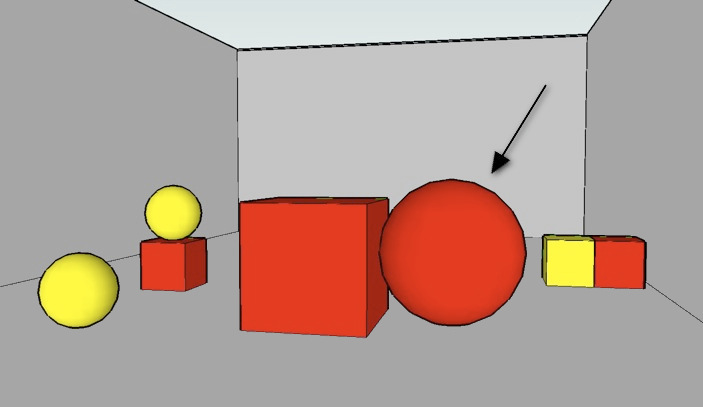
\includegraphics[width=\textwidth]{images/22sinletrasClaro.jpg}
  \caption{}\label{GRE3D7-stimulus1}
\end{subfigure}%
\begin{subfigure}{.5\textwidth}
 \centering
\begin{tabular}{l}
 {\it La esfera grande}\\

 {\it La esfera roja que est\'a al lado del cubo rojo} \\

 {\it El objeto que est\'a al lado del cubo grande}\\

 {\it La bola roja}\\

 {\it La pelota a la izquierda del cubo amarillo}\\

 {\it La bola grande}\\

 {\it La esfera que est\'a a la derecha del cubo rojo y a }\\
{\it la izquierda del cubo amarillo}\\

 {\it La cosa que est\'a a la derecha del cubo del medio}\\

  {\it ...}
 \end{tabular}
\hspace*{-30cm}
\centering\caption{}\label{er-figura1}
\end{subfigure}
\begin{centering}
\caption{Expresiones referenciales que identifican al objeto se\~nalado por la flecha.}
\label{figura-er}
\end{centering}
\end{figure}

La \textbf {generaci\'on de expresiones referenciales (GER)} entre todas las subtareas de GLN, es una de las que ha recibido m\'as atenci\'on. En la pr\'actica, la mayor\'ia de los sistemas de GLN, con independencia de su finalidad, contiene un m\'odulo de GER de alg\'un tipo~\cite{Mellish2004}. Esto no es sorprendente
en vista del papel central que las expresiones referenciales tienen en la comunicaci\'on. Un sistema que proporciona
consejos sobre los viajes a\'ereos \cite{white2010generating} tiene que hacer referencia a los vuelos ---{\it el vuelo m\'as barato}, {\it un vuelo directo}---, un sistema de navegaci\'on para autom\'oviles~\cite{Drager:2012:GLN:2380816.2380908}
necesita generar descripciones espaciales ---{\it tomar el puente junto a la iglesia, a la derecha}---,
y un robot que ensambla piezas de juguetes junto con un usuario humano~\cite{foster-etal-ijcai2009} debe hacer referencia a los componentes ---{\it inserte el perno verde hasta el final en el cubo rojo}. Cuando hablamos, nos referimos a cosas (tangibles como un puente, o intangibles como una fecha), es decir generamos expresiones referenciales. Un sistema que genera texto, tambi\'en deber\'a generar expresiones referenciales. La generaci\'on autom\'atica de expresiones referenciales es el tema de esta tesis.

Un sistema de GLN incluye 3 etapas: {\bf determinaci\'on de contenido} ---qu\'e decir--- {\bf lexicalizaci\'on} ---con qu\'e palabras--- y {\bf realizaci\'on ling\"{u}\'istica} ---c\'omo decirlo. La determinaci\'on de contenido, elige qu\'e informaci\'on incluir en la oraci\'on. La lexicalizaci\'on elige qu\'e lexemas usar para comunicar el contenido determinado por la etapa anterior. Y la realizaci\'on arma la oraci\'on agregando los art\'iculos, preposiciones, y dem\'as palabras funcionales necesarias y orden\'andolas de forma tal que la frase resultante sea gramaticalmente aceptable. 

Un sistema de GER, tiene esas 3 etapas tambi\'en: {\bf determinaci\'on de contenido} ---decide qu\'e propiedades o relaciones del objeto a describir se incluir\'an en la expresi\'on referencial--- {\bf lexicalizaci\'on} ---elige las palabras que se van a usar para nombrar las propiedades y relaciones--- y {\bf realizaci\'on ling\"u\'istica} ---se encarga de armar el sintagma nominal para que sea gramaticalmente correcto.

Por ejemplo, la primer ER de la Figura \ref{figura-er} incluye las propiedades {\it tama\~no} y {\it forma} del objeto se\~nalado por la flecha, lexicalizadas como {\it grande} y {\it esfera} respectivamente y realizadas agregando el art\'iculo {\it la} antes de {\it esfera}, e incluyendo el sustantivo {\it esfera} antes que el adjetivo {\it grande}; formando as\'i el sintagma nominal {\it La esfera grande} que es correcto en espa\~nol. Otra lexicalizaci\'on y realizaci\'on de las mismas propiedades ---es decir, de la misma sem\'antica--- podr\'ia ser {\it La bola de gran tama\~no}. A lo largo de esta tesis usaremos el t\'ermino {\bf expresi\'on referencial} (ER) para nombrar la salida de cualquiera de las 3 etapas de la GER. Es decir, llamaremos expresi\'on referencial al conjunto de propiedades y relaciones que refieren un\'ivocamente a un objeto aunque no est\'en lexicalizadas o realizadas.

En lo que sigue introduciremos terminolog\'ia b\'asica, relacionada con la GER que nos servir\'a a lo largo de toda la tesis para entendernos.

El {\bf dominio} de una ER define los tipos de entidades que est\'an siendo contemplados. Por ejemplo el dominio de la Figura \ref{figura-er} son las figuras geom\'etricas en 3 dimensiones. En particular, el dominio incluye cubos y esferas de colores rojo y amarillo, algunas grandes y otras peque\~nas, situadas en un entorno con perspectiva.

El {\bf contexto} de una ER contiene un subconjunto de las entidades del dominio. La Figura \ref{figura-er} muestra un contexto con 7 entidades del dominio, 4 rojas y 3 amarillas. Otros ejemplos son los puntos de referencia visibles en un cierto momento en un camino para el que estamos dando direcciones, un subconjunto de las fotograf\'ias utilizadas en una configuraci\'on experimental, o los ingredientes de cocina que ya se han mencionado en una receta. En un dominio visual, el contexto, incluyendo las propiedades de sus objetos y su configuraci\'on espacial, se puede llamar \textbf{escena}. %El contexto de la Figura \ref{GRE3D7-stimulus1} son los todos los objetos visibles con sus propiedades.

Cada {\bf entidad} del contexto (tambi\'en conocido como objeto o elemento) tiene un tipo ---\emph{esfera}--- ciertas propiedades o caracter\'isticas ---\emph{color}---, valores de esas propiedades ---\emph{rojo}---, y puede tener relaciones con otros objetos ---\emph{a la derecha de}. Una {\bf propiedad} (unaria) es una caracter\'istica de una entidad particular. Por ejemplo, la raza de un perro, el tener o no tener bigotes para un hombre, o el color para un objeto. Cada entidad puede tener muchas propiedades, y puede tener relaciones (tambi\'en llamadas: propiedades binarias), por ejemplo con respecto a la posici\'on f\'isica, como estar situado al lado de otro objeto. 

El {\bf target} (u objetivo), es el subconjunto de objetos de un contexto a los cuales queremos referirnos. En la escena del ejemplo de la Figura \ref{figura-er}, el target es el objeto se\~nalado por la flecha. En este caso, el target es un conjunto singleton, es decir tiene un s\'olo elemento. Si el target tiene m\'as de un elemento, las ERs que lo identifican son plurales.

Dado un contexto, un target y una descripci\'on (parcial) del target, los {\bf distractores} son otros elementos que se encuentran en el contexto, y que tambi\'en cumplen con la descripci\'on parcial. Si la descripci\'on parcial es {\it esfera} las esferas que no son el target de la Figura \ref{figura-er} son  distractores, y por ello es necesario seguir agregando propiedades o relaciones para identificar un\'ivocamente al target.

Un {\bf algoritmo} para GER, es un procedimiento autom\'atico que toma, al menos, alg\'un tipo de representaci\'on de un contexto y un target, y da como resultado una (o m\'as) expresi\'on(es) referencial(es) para el target considerado, si puede identificarlo un\'ivocamente en el contexto.

Una computadora que se enfrenta a la tarea de generar autom\'aticamente expresiones referenciales en un contexto determinado, necesitar\'a una representaci\'on de todos los objetos de la Figura \ref{figura-er} y las propiedades de cada uno de ellos. En la Figura~\ref{contexto-tabla-propiedades} se muestra una posible forma de representar los objetos, sus propiedades y relaciones: una base de datos que contiene todas las propiedades relevantes de los objetos de la escena. Entonces, la tarea de GER para el objeto $e_5$ involucra encontrar alguna combinaci\'on de valores de propiedades y relaciones con otros objetos, que aplique \'unicamente a $e_5$, y no a los otros objetos. Como dijimos, esta tarea de encontrar las propiedades y relaciones que aplican a un target y no a los distractores, se llama {\emph selecci\'on de contenido para la generaci\'on de una expresi\'on referencial}. Mirando la Tabla \ref{tabla-propiedades} podemos decir que {\it red ball}, {\it large ball} y {\it large red ball} son algunas ERs del objeto $e_5$, cuyas realizaciones en espa\~{n}ol podr\'ian ser: {\it La bola roja}, {\it La esfera grande} y {\it La esfera grande y roja}. {\it La bola roja} y {\it La esfera grande} aparecen entre las ERs dadas por las personas listadas en la Figura \ref{figura-er}.
%Como una primera intuici\'on podemos ver que la Figura \ref{formula-subgrafo} es un subrafo de la Figura \ref{representacion-modelo} que identifica un\'ivocamente al target, representa la cuarta ER mostrada en la Figura \ref{er-figura1}. Y la Figura \ref{formula-subgrafo2} tambi\'en identifica al target un\'ivocamente y representa la segunda ER mostrada en \ref{er-figura1}.
%que est\'an dadas en la Figura \ref{er-figura1} son muchas m\'as de las que mostramos en las f\'ormulas de la Figura \ref{er-figura1-b}, esto nos lleva a pensar que un algoritmo puede que no consiga la variedad que las personas dan. La representaci\'on ilustrada en la Figura~\ref{representacion-modelo} es equivalente a la mostrada en la Tabla \ref{tabla-propiedades}.

%\vspace*{-1.5cm}
\begin{figure}[h]
\begin{subfigure}{.45\textwidth}
  \centering
	\vspace*{-.2cm}
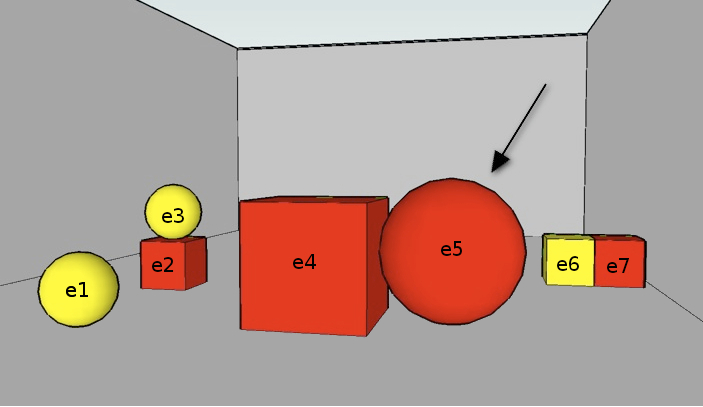
\includegraphics[width=\textwidth]{images/22.jpg}
  \caption{}\label{GRE3D7-stimulus1-ids}
\end{subfigure}
\begin{subfigure}{1\textwidth}
% \centering
%\begin{centering}
\hspace*{-16cm}
\begin{scriptsize}
\begin{tabular}{|l|c|c|c|c|c|c|c|}
\hline
\textbf {id}& 	\textbf {type}		&	\textbf {color}	&	\textbf {size}& \textbf {rigth} & \textbf {left} & \textbf {ontop}	& \textbf {below}	\\
   	   &  	    			&	    		&	     		&  \textbf {of}   		 &  \textbf {of}	    &  	&  \\
\hline \hline
$e_1$ & ball & yellow & small & - & - & - & - \\
$e_2$ & cube & red & small & - & - &- & $e_3$ \\
$e_3$ & ball & yellow & small & - & - & $e_2$ & -\\
$e_4$ & cube & red & large & - & $e_5$ & - & -\\
$e_5$ & ball & red & large & $e_4$ & - & - & -\\
$e_6$ & cube & yellow & small & - & $e_7$ & - & -\\
$e_7$ & cube & red & small & $e_6$ & - & - & -\\
\hline
%&&&&&&&\\
%&&&&&&&\\

\end{tabular}
\end{scriptsize}
\vspace*{1cm}
%\center
\centering \hspace*{-8cm} \caption{}\label{tabla-propiedades}
%\end{centering}
\end{subfigure}
\caption{Formalizaci\'on de las propiedades de la escena en una tabla de doble entrada.}\label{contexto-tabla-propiedades}
\end{figure}

En la pr\'oxima secci\'on veremos porqu\'e la tarea de GER es m\'as compleja de lo que parece a primera vista y en la siguiente introduciremos c\'omo herramientas de teor\'ia de modelos nos pueden ayudar.

\section{Expresiones referenciales bajo incertidumbre}
\label{sec:gre-incertidumbre}


%Los conjuntos son dif\'icil para referirse a, por ejemplo, y algoritmos
%diseñado para tratar con ellos lograr una menor semejanza humana cuando se refiere a los conjuntos de
%a los objetos individuales (van Deemter et al., en prensa). Los recientes esfuerzos para dejar que los algoritmos REG
%referirse a las regiones espaciales sugieren que en dominios grandes, realista, identificación precisa de
%un objetivo es un objetivo que se puede aproximar, pero rara vez alcanzado (Turner et al., 2008;
%Turner, Sripada, y Reiter 2009) .Es en tales dominios que prominencia (especialmente en el
%sentido no lingüístico) se convierte en un problema crítico. 
Cuando la generaci\'on de expresiones referenciales ocurre en la vida real, en lugar de ocurrir en un experimento controlado, las fuentes de \textbf{incertidumbre} que afectan al proceso se multiplican. En trabajo 
reciente en el \'area de GER \cite{turner2008,turner2009} se discute que, al intentar usar algoritmos de GER en dominios grandes 
y realistas (como por ejemplo la descripci\'on de regiones en mapas) la identificaci\'on precisa del target es una tarea que puede ser 
aproximada pero raramente lograda. Los autores argumentan que esto se debe, en parte, a que las representaciones geogr\'aficas 
son necesariamente \textbf{incompletas}. Esta falta de informaci\'on introduce incertidumbre (por ejemplo, el restaurante se\~nalado por la flecha en la Figura \ref{target_mapa}, ?`es realmente el \'unico restaurante de esa calle? o ?`es el \'unico que aparece en el mapa?).

\begin{figure}[h]
\centering
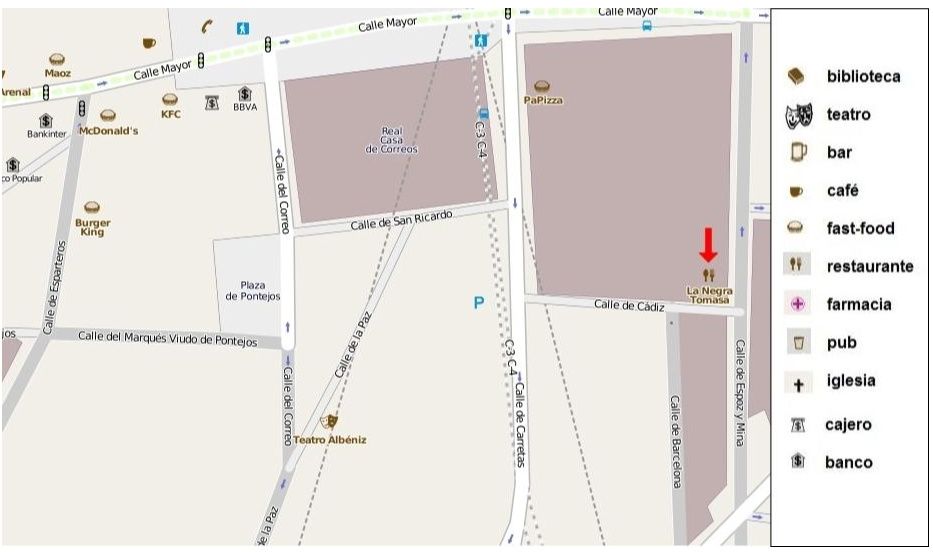
\includegraphics[width=\textwidth]{images/corpus/mapa15.png}
\caption{Ejemplo de target en el contexto de un mapa del ZOOM corpus.}
\label{target_mapa}
\end{figure}

Cuando la informaci\'on del contexto proviene de datos de sensores, las entradas del algoritmo de GER son inevitablemente ruidosas. Es decir, 
contienen informaci\'on no s\'olo incompleta sino tambi\'en posiblemente {\bf incorrecta}. Incluso en contextos tan simples como el de la 
Figura \ref{figura-er} hay incertidumbre. ?`La Figura \ref{representacion-modelo1} representa toda la informaci\'on del 
contexto?. Algunos podemos opinar que s\'i, otros que no. 

\begin{figure}[h]
%\begin{subfigure}{.5\textwidth}
  \centering
\vspace*{1cm}
\begin{picture}(250,50)
\put(0,-50){\begin{tikzpicture}
  [
    n/.style={circle,draw,inner sep=1.5pt,node distance=1.5cm},
		 aArrow/.style={->, >=stealth, semithick, shorten <= 1pt, shorten >= 1pt},
  ]
 \node[n,label=below:{
    \relsize{-2}$\begin{array}{c}
      \nSmall\\[-3pt] 
      \nYellow \\[-3pt] 
      \nBall\end{array}$}] (a) {$e_1$};
 \node[n,label=below:{
    \relsize{-2}$\begin{array}{c}     
      \nSmall\\[-3pt] 
      \nRed\\[-3pt] 
      \nCube\end{array}$}, right of=a] (b) {$e_2$};
 \node[n,label=above:{
    \relsize{-2}$\begin{array}{c}     
      \nSmall\\[-3pt] 
      \nYellow\\[-3pt] 
      \nBall\end{array}$}, above of=b] (c) {$e_3$};
 \node[n,label=below:{
    \relsize{-2}$\begin{array}{c}
      \nLarge\\[-3pt] 
      \nRed\\[-3pt] 
      \nCube\end{array}$}, right of=b] (d) {$e_4$};
 \node[n,label=below:{
    \relsize{-2}$\begin{array}{c}
      \nLarge\\[-3pt] 
      \nRed\\[-3pt] 
      \nBall\end{array}$}, right of=d] (e) {$e_5$};
 \node[n,label=below:{
    \relsize{-2}$\begin{array}{c}
      \nSmall\\[-3pt] 
      \nYellow\\[-3pt] 
      \nCube\end{array}$}, right of=e] (f) {$e_6$};
 \node[n,label=below:{
    \relsize{-2}$\begin{array}{c}
      \nSmall\\[-3pt]
      \nRed\\[-3pt] 
      \nCube\end{array}$},  right of=f] (g) {$e_7$};
 \draw [aArrow,bend right=40] (b) to node[auto,swap]{\relsize{-3}$\nBelow$} (c);
 \draw [aArrow,bend right=40] (c) to node[auto,swap]{\relsize{-3}$\nOntop$} (b);
 \draw [aArrow,bend right=40] (d) to node[auto,swap]{\relsize{-3}$\nLeftof$} (e);
 \draw [aArrow,bend right=40] (e) to node[auto,swap]{\relsize{-3}$\nRightof$} (d);
 \draw [aArrow,bend right=40] (f) to node[auto,swap]{\relsize{-3}$\nLeftof$} (g);
 \draw [aArrow,bend right=40] (g) to node[auto,swap]{\relsize{-3}$\nRightof$} (f);
 %\draw[dotted] (-0.5,-1.3) rectangle (8,3.1);
 \draw[dotted] (-0.5,-1.5) rectangle (8,3);
 \end{tikzpicture}}
 \end{picture}
 %\end{flushleft}

\vspace*{1.5cm} 
\caption{Formalizaci\'on de las propiedades de la Figura \ref{figura-er} como un grafo etiquetado.}\label{representacion-modelo1}
\end{figure}


En efecto, la persona que gener\'o la ER {\it La pelota a la izquierda del cubo amarillo} opina que no: la relaci\'on \emph{a la izquierda de} entre el target y el cubo amarillo no est\'a representada en el grafo. Un algoritmo de GER con este grafo como input no puede generar esta expresi\'on referencial. La informaci\'on disponible no s\'olo impide la generaci\'on de ERs v\'alidas, sino que tambi\'en permite la generaci\'on de ERs claramente incorrectas como \emph{La esfera roja 
que no tiene nada a la derecha}.
El grafo puede completarse para que sea posible
generar la expresi\'on referencial. El grafo resultante se ilustra en la Figura \ref{representacion-modelo-completo}. Sin embargo, este grafo tampoco es completo, 
de hecho, la ER {\it la cosa que est\'a a la derecha del cubo del medio} no se podr\'ia generar con este grafo. 

\begin{figure}[h]
%\begin{subfigure}{.5\textwidth}
\centering
%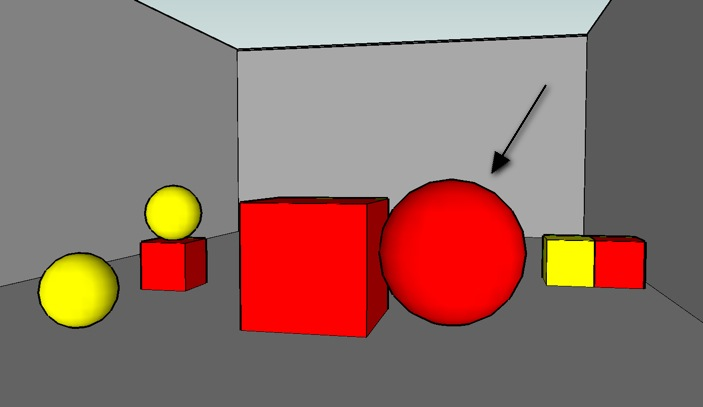
\includegraphics[width=\textwidth]{images/22sinletras.jpg}
%%\caption{Ejemplo de contexto}
%\label{GRE3D7-stimulus1-b}
\vspace*{1cm}
\begin{picture}(250,50)
\put(0,-50){\begin{tikzpicture}
  [
    n/.style={circle,draw,inner sep=1.5pt,node distance=1.5cm},
		 aArrow/.style={->, >=stealth, semithick, shorten <= 1pt, shorten >= 1pt},
  ]
 \node[n,label=below:{
    \relsize{-2}$\begin{array}{c}
      \nSmall\\[-3pt] 
      \nYellow \\[-3pt] 
      \nBall\end{array}$}] (a) {$e_1$};
 \node[n,label=below:{
    \relsize{-2}$\begin{array}{c}     
      \nSmall\\[-3pt] 
      \nRed\\[-3pt] 
      \nCube\end{array}$}, right of=a] (b) {$e_2$};
 \node[n,label=above:{
    \relsize{-2}$\begin{array}{c}     
      \nSmall\\[-3pt] 
      \nYellow\\[-3pt] 
      \nBall\end{array}$}, above of=b] (c) {$e_3$};
 \node[n,label=below:{
    \relsize{-2}$\begin{array}{c}
      \nLarge\\[-3pt] 
      \nRed\\[-3pt] 
      \nCube\end{array}$}, right of=b] (d) {$e_4$};
 \node[n,label=below:{
    \relsize{-2}$\begin{array}{c}
      \nLarge\\[-3pt] 
      \nRed\\[-3pt] 
      \nBall\end{array}$}, right of=d] (e) {$e_5$};
 \node[n,label=below:{
    \relsize{-2}$\begin{array}{c}
      \nSmall\\[-3pt] 
      \nYellow\\[-3pt] 
      \nCube\end{array}$}, right of=e] (f) {$e_6$};
 \node[n,label=below:{
    \relsize{-2}$\begin{array}{c}
      \nSmall\\[-3pt]
      \nRed\\[-3pt] 
      \nCube\end{array}$},  right of=f] (g) {$e_7$};
 \draw [aArrow,bend right=40] (b) to node[auto,swap]{\relsize{-3}$\nBelow$} (c);
 \draw [aArrow,bend right=40] (c) to node[auto,swap]{\relsize{-3}$\nOntop$} (b);
 \draw [aArrow,bend right=40] (d) to node[auto,swap]{\relsize{-3}$\nLeftof$} (e);
 \draw [aArrow,bend right=40] (e) to node[auto,swap]{\relsize{-3}$\nRightof$} (d);
 \draw [aArrow,bend right=40] (f) to node[auto,swap]{\relsize{-3}$\nLeftof$} (g);
 \draw [aArrow,bend right=40] (g) to node[auto,swap]{\relsize{-3}$\nRightof$} (f);
 
 \draw [aArrow,bend right=40] (a) to node[auto,swap]{} (b);
 \draw [aArrow,bend right=40] (b) to node[auto,swap]{} (a);

 \draw [aArrow,bend right=40] (b) to node[auto,swap]{} (d);
 \draw [aArrow,bend right=40] (d) to node[auto,swap]{} (b);

\draw [aArrow,bend right=40] (e) to node[auto,swap]{} (f);
 \draw [aArrow,bend right=40] (f) to node[auto,swap]{} (e);
 %\draw[dotted] (-0.5,-1.3) rectangle (8,3.1);
 \draw[dotted] (-0.5,-1.5) rectangle (8,3);
 \end{tikzpicture}}
 \end{picture}
 %\end{flushleft}

\vspace*{2cm} 
 \caption{Representaci\'on de contexto m\'as completo.}\label{representacion-modelo-completo}
\end{figure}


Aunque no hablemos ni de incompletitud ni de incorrectitud tambi\'en hay incertidumbre en \textbf{cu\'al} de todas las posibles ERs un sistema de GER debe 
elegir. Por ejemplo seguramente hay personas que preferir\'an ERs que usen la palabra \emph{esfera}, antes que \emph{bola}. Y seguramente 
no falte quien diga que \emph{la} mejor expresi\'on referencial ni si quiera aparece en la Figura \ref{figura-er}. Sin embargo, seguramente 
habr\'a una tendencia como se muestra en estudios previos \cite{viet:gene11}. Nadie preferir\'a una ER que use 21 propiedades y 6 relaciones 
para describir al target de la Figura \ref{figura-er}.

El largo de una ER afecta su calidad. Se podr\'{i}a pensar, por ejemplo, que las referencias son \'optimas cuando son \textbf{m\'{i}nimas}
 en longitud, es decir, cuando contienen s\'olo informaci\'on suficiente para identificar el objeto target y nada m\'as. Pero la generaci\'on de referencias m\'{i}nimas
no es lo que las personas hacen ni lo que es m\'as \'util para los oyentes, como se muestra en trabajo previo \cite{Lu_sasha2015}. Y ni si quiera 
nos resuelve el problema de elegir una ER. {\it La bola grande} y {\it La esfera roja} son dos ERs de la Figura \ref{figura-er} y tienen 
exactamente la misma longitud.

Dado que la incertidumbre es inherente a la tarea de GER, lo mejor que se puede hacer es que un algoritmo de GER devuelva un \textbf{ranking}
 de ERs, o lo que es lo mismo, un conjunto de ERs en el que cada ER tiene un valor asociado que intenta reflejar cu\'an buena es esa ER para el input dado.

?`Como podemos generar un ranking de ERs?.
Un algoritmo simplista generar\'ia primero todas las ERs posibles y luego las ordenar\'ia con alg\'un criterio. Esto es posible porque la cantidad de ERs es finita dado un modelo finito, pero esta cantidad puede ser muy grande, exponencial en el tama\~{n}o del modelo y la gran mayor\'ia de estas ERs no se llegar\'ian a usar en una aplicaci\'on real. Una aplicaci\'on s\'olo usar\'a las mejores ERs de un target considerado.
Una forma m\'as eficiente de generar un ranking de ERs es dise\~{n}ar un algoritmo no determin\'istico y correrlo una cantidad de veces suficiente para la aplicaci\'on.

Un algoritmo para la GER es {\bf no-determin\'istico} si puede dar diferentes ERs para el mismo contexto y target en sucesivas ejecuciones. 
Para producir un ranking de las mejores ERs para un target, el no determinismo debe estar guiado de alguna forma que le permita dar m\'as veces ERs m\'as frecuentes, y menos veces las menos frecuentes. Llamaremos a esta gu\'ia: \textbf{probabilidad de uso} de una propiedad o relaci\'on. Esta probabilidad se puede ver afectada por caracter\'isticas de la propiedad o relaci\'on (tipos de propiedades) o por caracter\'isticas de qui\'en interpretar\'a la ER (el interlocutor).

Hay diferentes \textbf{tipos de propiedades}, por ejemplo taxon\'omicas (las que tiene el objeto, como \emph{esfera}, o \emph{roja}), relacionales (las que necesitan dar una expresi\'on de otro objeto, por ejemplo {\it estar al lado de}), vagas (son las m\'as dif\'iciles de identificar, por ejemplo: \emph{chico}, \emph{grande}, no son propiedades absolutas, ya que necesitan un contexto, ?`con respecto a qu\'e algo es chico o grande?). Ciertos valores de propiedades pueden ser m\'as f\'aciles de identificar que otros, por ejemplo cierto color verde podr\'{i}a ser m\'as complicado de identificar que el tama\~no grande de un objeto. Notar que cuando decimos el tama\~no, tenemos como marco de referencia a los objetos de la escena, en ese contexto un objeto es {\it grande}.
%En esta tesis estudiamos la generaci\'on autom\'atica de expresiones referenciales, 
%primero mostramos c\'omo podemos a\~nadir no determinismo a los algoritmos estudiados. Los algoritmos de refinamiento estudiados, tienen un orden fijo en el cual consideran las propiedades y relaciones, y la naturalidad de las expresiones referenciales que generan depende de este orden particular considerado, nosotros proponemos reemplazar ese orden fijo sobre las propiedades y/o relaciones de la escena de entrada por una~\emph{probabilidad de uso} para cada propiedad y/o relaci\'on, y modificar los algoritmos para que tengan en cuenta esas propiedades. De esta manera, cada llamada al algoritmo puede producir diferentes ERs para la misma escena y target de entrada. 

%Es decir nuestra meta, no s\'olo ser\'a crear algoritmos para la generaci\'on autom\'atica de expresiones referenciales, sino crearlos de tal manera que podamos imitar en gran medida lo que dir\'ian las personas.
%
%Mostraremos que dado un corpus (como el corpus GRE3D7 o el TUNA de los cuales hablaremos en Cap\'itulo~\ref{sec:seleccion}) podemos estimar estas probabilidades de uso de manera que las ER se generen con una distribuci\'on de probabilidad que coincide en gran medida con las que se encuentra en el corpus.

Esta selecci\'on de la ER m\'as apropiada tambi\'en debe tener en cuenta al \textbf {interlocutor}, es natural que los humanos demos distintas ERs a distintos interlocutores.
% En el \'area muchas veces se habla de optimalidad de la ER, pero con diferentes significados, para algunos una ER \'optima es aquella que dice lo m\'inimo necesario para identificar al objeto target, para otros es la menos esfuerzo requiere del interlocutor para identificarlo.
La selecci\'on de qu\'e propiedades y/o relaciones con otros objetos incluir en una expresi\'on referencial depender\'a del prop\'osito que tengamos para dicha expresi\'on referencial. Una expresi\'on referencial ser\'a muy distinta si nuestro objetivo es dar la m\'inima informaci\'on que distinga al objeto, que si nuestro objetivo es ayudar al interlocutor a que identifique el objeto.

La generaci\'on de expresiones referenciales en el mundo real sufre de diversas fuentes de incertidumbre. En esta tesis proponemos formas para modelar esta incertidumbre partiendo de t\'ecnicas de representaci\'on de conocimiento basadas en teor\'ia de modelos.
%En la vida real hay muchas cosas que nos ayudan a darnos cuenta si nuestro interlocutor identific\'o el objeto target, como ser la expresi\'on de duda nos dar\'ia una pauta de que no esta entendiendo lo que le queremos decir...
%
%\textbf{FALTA CIERRE A ESTA SECCION!}

%En esta tesis nos vamos a enfocar en la selecci\'on de contenidos de las expresiones referenciales, y el objetivo ser\'ia simular el comportamiento humano, para ello vamos a usar corpus de expresiones referenciales para aprender como realizan esta tarea las personas.
 %
%Las propiedades y relaciones de los objetos de la escena forman una base de conocimento, estos datos se pueden organizar en jerarqu\'ias, por ejemplo: conjunto de animales, conjunto de mamiferos, conjunto de insectos. Algunos conjuntos pueden estar contenidos en otros, es decir algunos objetos o entidades pueden compartir caracter\'isticas.
%
%Si el objeto target tiene la propiedad de medir 1.80 de alto, y est\'a en un grupo donde los dem\'as son m\'as peque\~nos, es m\'as natural decir el m\'as alto, que el que mide 1.80.
%Si tenemos 100 caracter\'isticas de una persona, y con esas caracter\'isticas se pudiera identificar un\'ivocamente a una persona, un sistema que diera que las 100 caracter\'isticas no ser\'ia un sistema que suene muy natural, ya que una persona no dar\'ia 100 propiedades para identificar a una persona particular. As\'i podr\'iamos decir que las expresiones referenciales variaran seg\'un la cantidad de informaci\'on que contienen, si contienen la m\'inima informaci\'on para identificarlas un\'ivocamente ser\'an minimales, si contienen m\'as informaci\'on estar\'an sobreespecificadas, pero en el caso de contener m\'as de la m\'inima informaci\'on para identificarlas un\'ivocamente... cu\'anta m\'as dar?, intentaremos imitar lo que hacen las personas cuando dan expresiones referenciales para responder este tipo de preguntas.
%El sistema deber\'ia tener una lista del orden de preferencia de los atributos a usar.\\ 



%NO NO Las primeras investigaciones en GER no voy a poner esto porque no quiero pasar por alto shrdlu de vinogran 1969
%\cite{C92-1038}; \cite{Dale95computationalinterpretations} hicieron una serie de supuestos simplificadores, por ejemplo no usaban relaciones, el target era un s\'olo objeto, y como resultado los primeros
%algoritmos GER s\'olo pod\'ian generar una variedad limitada de expresiones referenciales. Cuando
%los investigadores comenzaron a levantar algunos de estos supuestos, esto di\'o lugar a algoritmos de GER
%con un repertorio m\'as amplio, siendo capaces de generar, por ejemplo, plurales y expresiones relacionales. 
%
%Este movimiento ha creado una serie de nuevos desaf\'ios, sin embargo. Por ejemplo, el
%n\'umero de formas en las que uno puede referirse a un conjunto de objetos de destino aumenta, por lo que la elecci\'on de una
%buena expresi\'on referencial es m\'as dif\'icil.
%
%Del mismo modo, incluso propuestas recientes tienden a asumir que no es problem\'atico para determinar qu\'e informaci\'on
%es compartida entre el hablante y el oyente.\\
%(a) C\'omo se representa la informaci\'on del dominio?\\
%(b) C\'omo se representa el contenido sem\'antico de una expresi\'on referencial? \\
%(c) C\'omo se pueden encontrar descripciones distintivas?
%
%En los contextos de los corpus analizados en esta tesis, nos encontramos con cuatro tipos diferentes de atributos:
%tipos de objetos, atributos absolutos, atributos relativos, atributos espaciales incluidas las relaciones y atributos de localizaci\'on.
%
%El tipo de un objeto constituye un caso especial, ya que es muy rara vez omite
%en la expresi\'on referencial. En consecuencia, la mayor\'ia de los algoritmos tratan de
%considerarlo por separado para asegurarse de que se a\~nade a cada expresi\'on referencial. Una explicaci\'on parcial para esta condici\'on especial es que las expresiones referenciales se realizan como sintagmas nominales,
%cada sintagma nominal requiere un sustantivo, y por lo general es el tipo del referente dado que es el sustantivo principal.
%
%\section{Contribuciones de esta tesis}
%\label{sec:contribiciones}
%\textcolor{blue}{Esta parte se va?}
%\begin{itemize}
%\item Se estudi\'o el avance en el \'area de la generaci\'on autom\'atica de expresiones referenciales, los algoritmos existentes y los problemas que ellos ten\'ian, las aproximaciones emp\'iricas realizadas en el \'area en el Cap\'itulo~\ref{sec:seleccion}.
%\item Se estudiaron las m\'etricas de evaluaci\'on tanto autom\'aticas como manuales en el Cap\'itulo~\ref{sec:seleccion}, las cuales ser\'an luego aplicadas en el Cap\'itulo~\ref{sec:evaluacion}.
%%\item Se abordaron los siguientes problemas: no-determinismo, sobreespecificaci\'on.
%\item Se estudiaron estudiaron distintas l\'ogicas y sus lenguajes asociados, se compararon esos lenguajes con el lenguaje utilizado para dar ER, a fin de elegir una l\'ogica apropiada en el Cap\'itulo~\ref{sec:intro_logica}.
%\item Se seleccion\'o un algoritmo existente al cual se le agregaron probabilidades de uso para simular el no-determinismo encontrado en corpus. Este fue seleccionado por permitirmos agregar los aspectos tenidos en cuenta en esta tesis: dar un algoritmo que aborde el no-determinismo, la sobreespecificaci\'on que sea relacional, que genere plurales en el Cap\'itulo~\ref{sec:learning}.
%%\item Se modific\'o el algoritmo para que sea no-determinista.
%\item Se agreg\'o sobreespecificaci\'on al algoritmo permitiendo agregar propiedades o relaciones cuando estas tienen una alta probabilidad de uso en corpus. Y al mismo tiempo se agura la terminaci\'on en el Cap\'itulo~\ref{sec:algoritmo}.
%\item Se propone un m\'etodo para calcular las probabilidades de uso (\puse)\ de las relaciones del modelo el cual genera una distribuci\'on de expresiones referenciales cercana a la encontrada en el corpus.
%\item Se prob\'o el algoritmo en 2 corpus existentes (el GRE3D7 y el Tuna corpus) en el Cap\'itulo~\ref{sec:evaluacion}.
%\item Se realiz\'o una evaluaci\'on en la que se compararon las salidas del algoritmo con ambos corpus. Se usaron m\'etricas autom\'aticas y manuales Cap\'itulo~\ref{sec:evaluacion}.
%\item Se creo un corpus de descripciones de mapas (el ZOOM corpus).
%\item Se hizo un caso de estudio de 3 mapas del ZOOM corpus explicado en Cap\'itulo~\ref{sec:corpus}, en el cual se toma 1 mapa con target singular, el mismo mapa con zoom 2x y target singular y el mismo mapa con target plural.
%\end{itemize}



\section{Expresiones referenciales usando teor\'ia de modelos}
\label{sec:gre-teoria-modelos}

Los \textbf{modelos relacionales} tambi\'en conocidos como \textbf{modelos de kripke} y \textbf{modelos de primer orden} son muy utilizados para la representaci\'on de situaciones o escenas. 
Los modelos relacionales son grafos etiquetados y pueden verse tambi\'en como aut\'omatas finitos. Estas estructuras matem\'aticas han sido muy estudiadas y tienen muchas propiedades bien conocidas \cite{arec:hybr05b}. En esta tesis se adaptan algoritmos cl\'asicos de minimizaci\'on de aut\'omatas aplicados a la caracterizaci\'on de modelos relacionales.

Para un \textbf{vocabulario} de s\'imbolos relacionales r, un modelo relacional $\+M$ es una tupla $\tup{\Delta,\interp{\cdot}}$ donde:
\begin{itemize}
 \item $\Delta$ es un conjunto no vac\'io de objetos ---el dominio---
 \item $\interp{\cdot}$ es una funci\'on de interpretaci\'on, esto es, $\interp{r} \subseteq \Delta^n$ para todo s\'imbolo de relaci\'on $n$-ario $r$ que est\'a en el vocabulario.  
\end{itemize}
El \emph{tama\~no} de un modelo $\+M$ es la suma ($\#\Delta + \#\interp{\cdot}$), donde $\#\Delta$ es la cardinalidad
de $\Delta$ y $\#\interp{\cdot}$ es la suma de todas las aridades de las relaciones en $\interp{\cdot}$.
Si asumimos un vocabulario finito de s\'imbolos de relaci\'on $n$-arios entonces $\+M$ es \emph{finito}. 


%Un modelo relacional $\+M$ es una tupla 
%$\tup{\Delta,\interp{\cdot}}$ donde $\Delta$ es un conjunto no vac\'io, y
%$\interp{\cdot}$ es una funci\'on de interpretaci\'on, esto es,
%$\interp{r} \subseteq \Delta^n$ para todo s\'imbolo de relaci\'on $n$-aria tal que
%$r$ est\'a en el vocabulario. $\+M$ es \emph{finito} cuando
%$\Delta$ es finito.  El \emph{tama\~no} de un modelo $\+M$ es la suma
%$\#\Delta + \#\interp{\cdot}$, donde $\#\Delta$ es la cardinalidad
%de $\Delta$ y $\#\interp{\cdot}$ es la suma de todas las aridades de las
%relaciones en $\interp{\cdot}$.

A continuaci\'on vamos a presentar 2 ejemplos de modelos relacionales, uno en el que tenemos entidades \textbf{agentivas} (es decir, agentes animados que pueden realizar acciones) como perros y gatos, y otro en el que las entidades son \textbf{no agentivas}, es decir, son objetos est\'aticos.

El primer ejemplo se muestra en la Figura~\ref{fig:cat-dog-1} en la cual hemos representado un contexto
como un modelo relacional. Intuitivamente, $a$, $b$ y $d$ son perros, mientras que 
$c$ y $e$ son gatos;  $d$ es un peque\~no beagle; $b$ y $c$ tambi\'en son peque\~nos.
 Leeremos $\aSniffing(d,e)$ como ``{\em $d$ huele a $e$}''. La interpretaci\'on del s\'imbolo relacional $\nDog$ es $\interp{\nDog}$  =  $\cset{a,b,d}$ ya que $a$, $b$ y $d$ son los \'unicos perros del contexto. La interpretaci\'on de $\aSniffing$ es el conjunto de pares de elementos que cumplen $\aSniffing$. Por ejemplo ($a,a$) pertenece al conjunto dado que $a$ es un perro que se huele a s\'i mismo en el modelo.

 \begin{figure}[!ht]
 %\begin{center}
 \begin{tabular}{rcl}
$\Delta$               & = & $\cset{a,b,c,d,e}$\\
$\interp{\nDog}$      & = & $\cset{a,b,d}$\\
$\interp{\nCat}$      & = & $\cset{c,e}$\\
$\interp{\nBreed}$    & = & $\cset{d}$\\
$\interp{\aSmall}$    & = & $\cset{b,c,d}$\\
$\interp{\aSniffing}$ & = & $\cset{(a,a),(b,a),(c,b),(d,e),(e,d)}$
 \end{tabular}
\begin{picture}(90,30)
\put(0,-40){\begin{tikzpicture}
  [
    n/.style={circle,draw,inner sep=1.5pt,node distance=1.5cm},
    aSniffing/.style={->, >=stealth, semithick, shorten <= 3pt, shorten >= 3pt},
  ]
 \node[n,label=below:{\relsize{-1}$\begin{array}{c}\nDog\end{array}$}] (a) {$a$};

 \node[n,label=below:{\relsize{-1}$\begin{array}{c}\nDog\\ \aSmall \end{array}$}, right of=a] (b) {$b$};

 \node[n,label=below:{\relsize{-1}$\begin{array}{c}\nCat\\ \aSmall\end{array}$}, right of=b] (c) {$c$};

 \node[n,label=below:{\relsize{-1}$\begin{array}{c}\nDog\\ \nBreed\\  \aSmall \end{array}$}, right of=c] (d) {$d$};

 \node[n,label=below:{\relsize{-1}$\begin{array}{c}\nCat\end{array}$},right of=d] (e) {$e$};

 \draw [aSniffing,loop left] (a) to node[above,xshift=-5pt]{\relsize{-1}$\aSniffing$} (a);

 \draw [aSniffing,bend right=40] (b) to node[auto,swap]{\relsize{-1}$\aSniffing$} (a);

 \draw [aSniffing,bend right=40] (c) to node[auto,swap]{\relsize{-1}$\aSniffing$} (b);

 \draw[aSniffing, bend left=40] (d) to node[auto]{\relsize{-1}$\aSniffing$} (e);
 \draw[aSniffing, bend left=40] (e) to node[auto,swap]{\relsize{-1}$\aSniffing$} (d);

 \end{tikzpicture}}
 \end{picture}

 %\end{center}
 \caption{Representaci\'on de escena como un modelo relacional e interpretaci\'on de sus propiedades y relaciones. Ejemplo con entidades agentivas.\label{fig:cat-dog-1}}
 \end{figure}

El segundo ejemplo se muestra en la Figura~\ref{grafo-GRE3D7-stimulus_b} donde damos una posible representaci\'on de la escena de la Figura \ref{figura-er} como un modelo relacional. El dominio es $\Delta$  = $\cset{e_1,e_2,e_3,e_4,e_5,e_6,e_7}$. La interpretaci\'on de $\nBall$ es $e_1$, $e_3$ y $e_5$, ya que estos objetos son esferas, la de $\nCube$ es $\interp{\nCube}$ =$\cset{e_2, e_4, e_6, e_7}$, ya que esos objetos son cubos. Tenemos las relaciones $\nRightof$, $\nLeftof$, $\nBelow$ y $\nOntop$, cuyas interpretaciones se muestran en la figura. Como discutimos en la secci\'on anterior, se puede argumentar que este modelo est\'a incompleto, pero es suficiente para los objetivos ilustrativos de esta secci\'on.

\begin{figure}
\begin{flushleft}
\begin{tabular}{rcl}
$\Delta$              & = & $\cset{e_1,e_2,e_3,e_4,e_5,e_6,e_7}$\\
$\interp{\aRed}$      & = & $\cset{e_2,e_4,e_5,e_7}$\\
$\interp{\aYellow}$   & = & $\cset{e_1,e_3,e_6}$\\
$\interp{\nBall}$     & = & $\cset{e_1,e_3,e_6}$\\
$\interp{\nCube}$     & = & $\cset{e_2,e_4,e_6,e_7}$\\

$\interp{\aSmall}$    & = & $\cset{e_1,e_2,e_3,e_6,e_7}$\\
$\interp{\aLarge}$    & = & $\cset{e_4,e_5}$\\

$\interp{\nRightof}$   & = & $\cset{(e_4,e_5),(e_6,e_7)}$\\
$\interp{\nLeftof}$    & = & $\cset{(e_5,e_4),(e_7,e_6)}$\\
$\interp{\nOntop}$     & = & $\cset{(e_3,e_2)}$\\
$\interp{\nBelow}$     & = & $\cset{(e_2,e_3)}$\\

 \end{tabular}
\begin{picture}(120,50)
\put(0,-50){\begin{tikzpicture}
  [
    n/.style={circle,draw,inner sep=1.5pt,node distance=1.5cm},
		 aArrow/.style={->, >=stealth, semithick, shorten <= 1pt, shorten >= 1pt},
    %aSniffing/.style={->, >=stealth, semithick, shorten <= 3pt, shorten >= 3pt},
  ]
%\begin{tikzpicture}
%  [
%    n/.style={circle,fill,draw,inner sep=3pt,node distance=2cm},
%    aArrow/.style={->, >=stealth, semithick, shorten <= 1pt, shorten >= 1pt},
%  ]
 \node[n,label=below:{
    \relsize{-2}$\begin{array}{c}
      \nSmall\\[-3pt] 
      \nYellow \\[-3pt] 
      \nBall\end{array}$}] (a) {$e_1$};
 \node[n,label=below:{
    \relsize{-2}$\begin{array}{c}     
      \nSmall\\[-3pt] 
      \nRed\\[-3pt] 
      \nCube\end{array}$}, right of=a] (b) {$e_2$};
 \node[n,,label=above:{
    \relsize{-2}$\begin{array}{c}
      \nSmall\\[-3pt] 
      \nYellow\\[-3pt] 
      \nBall\end{array}$}, above of=b] (c) {$e_3$};
 \node[n,label=below:{
    \relsize{-2}$\begin{array}{c}
      \nLarge\\[-3pt] 
      \nRed\\[-3pt] 
      \nCube\end{array}$}, right of=b] (d) {$e_4$};
 \node[n,label=below:{
    \relsize{-2}$\begin{array}{c}
      \nLarge\\[-3pt] 
      \nRed\\[-3pt] 
      \nBall\end{array}$}, right of=d] (e) {$e_5$};
 \node[n,,label=below:{
    \relsize{-2}$\begin{array}{c}
      \nSmall\\[-3pt] 
      \nYellow\\[-3pt] 
      \nCube\end{array}$}, right of=e] (f) {$e_6$};
 \node[n,label=below:{
    \relsize{-2}$\begin{array}{c}
      \nSmall\\[-3pt]
      \nRed\\[-3pt] 
      \nCube\end{array}$},  right of=f] (g) {$e_7$};
 \draw [aArrow,bend right=40] (b) to node[auto,swap]{\relsize{-3}$\nBelow$} (c);
 \draw [aArrow,bend right=40] (c) to node[auto,swap]{\relsize{-3}$\nOntop$} (b);
 \draw [aArrow,bend right=40] (d) to node[auto,swap]{\relsize{-3}$\nLeftof$} (e);
 \draw [aArrow,bend right=40] (e) to node[auto,swap]{\relsize{-3}$\nRightof$} (d);
 \draw [aArrow,bend right=40] (f) to node[auto,swap]{\relsize{-3}$\nLeftof$} (g);
 \draw [aArrow,bend right=40] (g) to node[auto,swap]{\relsize{-3}$\nRightof$} (f);
 
%\draw[dotted] (-0.5,-1.3) rectangle (8,3.1);

% \end{tikzpicture}
%\caption{Grafo del contexto \ref{GRE3D7-stimulus}}
%\label{grafo-GRE3D7-stimulus_b}
%\end{figure}
 \end{tikzpicture}}
 \end{picture}
 \end{flushleft}
 \caption{Representaci\'on de la escena de la Figura \ref{figura-er} como un modelo relacional e interpretaci\'on de sus propiedades y relaciones. Ejemplo con entidades no agentivas.}
 \label{grafo-GRE3D7-stimulus_b}
 \end{figure}

Ahora nos enfocaremos en conseguir ERs para identificar a targets dados usando los modelos que acabamos de describir. Veremos lenguajes de distintas l\'ogicas y c\'omo las f\'ormulas l\'ogicas pueden representar a las ERs.
%Los lenguajes l\'ogicos son \'utiles para la tarea de describir (formalmente) elementos de una estructura relacional. 
A continuaci\'on definimos el lenguaje cl\'asico de la l\'ogica de primer orden (con desigualdad), \FOL. Dicho lenguaje se define inductivamente como sigue. Una f\'ormula $\phi$ es una f\'ormula de \FOL si es de alguna de las siguientes formas:

% *2 est\'a dado por $\top$ que es como decir 'cosa', todo elemento satisface $\top$, la desigualdad entre 2 elementos $ x_i$ y $x_j$, relaciones de tuplas, la negaci\'on de f\'ormulas de \FOL, la conjunci\'on de f\'ormulas de \FOL, y el existencial de una variable ligada en la f\'ormula de \FOL:
\begin{enumerate}
  \item $\top$ Es como decir {\it cosa}, todo elemento satisface $\top$.
  \item $x_i \not\approx x_j$ La desigualdad entre dos elementos $x_i$ y $x_j$.
  \item $r (\bar x)$ Relaciones de tuplas.
  \item $\lnot \gamma$ Negaci\'on de f\'ormulas.
  \item $\gamma \land \gamma'$ Conjunci\'on de f\'ormulas.
  \item $\exists x_i . \gamma$ Existencial de una variable ligada en la f\'ormula $\gamma$.
\end{enumerate}
%
donde $\gamma,\gamma' \in \FOL$,
$r$ es un s\'imbolo de relaci\'on $n$-aria y $\bar x$ es una tupla de $n$ variables.
Como es usual, $\gamma \lor \gamma'$ y $\forall x . \gamma$ son las versiones cortas de
$\lnot(\lnot\gamma \land \lnot\gamma')$ y $\lnot\exists x . \lnot\gamma$, respectivamente.
F\'ormulas de la forma $\top$, $x_i \not\approx x_j$ y $r(\bar
x)$ son llamados \emph{\'atomos}.%

Dado un modelo relacional $\+M = \tup{\Delta,\interp{\cdot}}$ y una
f\'ormula $\gamma$ con variables libres%
\footnote{%
    Asumimos que cada variable no puede aparecer libre y ligada a la vez, que una variable no est\'a ligada 2 veces,
    y que el \'indice de las variables crece en la f\'ormula de izquierda a derecha.%
}
$x_1\ldots x_n$, inductivamente definimos la \textbf{extensi\'on} o
\textbf{interpretaci\'on} de $\gamma$ como el conjunto de $n$-tuplas
 $\interp{\gamma}^n \subseteq \Delta^n$ que satisface:

\begin{enumerate}

\item $\interp{\top}^n$ $=$ $\Delta^n$

\item $\interp{x_i \not\approx x_j}^n$ $=$ $\cset{\bar{a} \mid \bar{a} \,{\in}\, \Delta^n, a_i \neq a_j}$

\item $\interp{\lnot\delta}^n$ $=$ $\Delta^n \setminus \interp{\delta}^n$

\item $\interp{r (x_{i_1} \ldots x_{i_k})}^n$ $=$ $\cset{\bar{a} \mid \bar{a} \,{\in}\, \Delta^n, (a_{i_1} \ldots a_{i_k}) {\in} \interp{r}}$

\item $\interp{\delta \land \theta}^n$ $=$ $\interp{\delta}^n \cap \interp{\theta}^n$

\item $\interp{\exists x_{l}.\delta}^n$ $=$ $\cset{\bar a \mid \bar a  e  \in \interp{\delta'}^{n+1}\ \text{para alg\'un elemento $e$}}$

\end{enumerate}

donde $1 \le i,j, i_1, \ldots, i_k \le n$, $\bar{a} = (a_1\ldots
a_n)$, $\bar{a}e = (a_1\ldots a_n,e)$ y $\delta'$ son
obtenidos reeplazando todas las ocurrencias de $x_l$ en $\delta$ por
$x_{n+1}$. 
%Cuando la cardinalidad de las tuplas involucradas en el contexto es conocida 
%escribiremos $\interp{\phi}$ en lugar de
%$\interp{\phi}^n$.

Con una sintaxis y sem\'antica de un lenguaje en mente, podemos formalmente definir el problema de \textbf{GER en $\gL$} ($\gL$-GER) para un conjunto target de elementos $T$. $\gL$ es el lenguaje de la l\'ogica elegida, en este caso hemos explicado la l\'ogica de primer orden $\FOL$, y en el Cap\'itulo \ref{sec:intro_logica} restringiremos esa l\'ogica para obtener ERs m\'as cercanas a las que aparecen en corpora y para conseguir algoritmos computacionalmente m\'as eficientes.

\medskip
\noindent
{\small
\begin{center}
\begin{tabular}{ll} \hline
\multicolumn{2}{l}{
\textsc{Problema $\gL$-GER }}\\ \hline
\ \ Entrada: & un modelo $\gM=\tup{\Delta,\interp{\cdot}}$ y un conjunto target no vac\'io $T \subseteq \Delta$.\\
\ \ Salida: & una f\'ormula $\varphi \in \gL$ tal que
$\interp{\varphi} = T$ si existe, y $\bot$ caso contrario.\\ \hline
\end{tabular}
\end{center}}

La salida del problema $\+L$-GER es una f\'ormula de
$\+L$ cuya interpretaci\'on en el modelo de input $\gM$ es el conjunto target $T$, si
esa f\'ormula existe. 
Cuando la salida no es $\bot$, decimos que $\phi$ es una
\textbf{expresi\'on referencial en $\+L$ (ER-$\+L$)} para $T$ en $\+M$, y cuando es $\bot$ puede ser que la l\'ogica elegida no sea lo suficientemente expresiva para identificar al target, o que el modelo dado no tenga suficiente detalle.

Consideramos s\'olo modelos relacionales con s\'imbolos de relaciones unarias y binarias, usaremos $p$ para las proposiciones (propiedades) y $r$ para los s\'imbolos de relaci\'on binarias.
Como dijimos anteriormente, dado un modelo $\gM$, podr\'ia haber un n\'umero muy grande de f\'ormulas que de forma un\'ivoca
describan al target (incluso f\'ormulas que no son l\'ogicamente equivalentes podr\'ian tener
la misma interpretaci\'on una vez que el modelo este fijo). Por ejemplo, en el modelo $\+M$ de la Figura \ref{grafo-GRE3D7-stimulus_b} las f\'ormulas $\aLarge \land \nBall$ y $\aRed \land \nBall$ no son l\'ogicamente equivalentes pero tienen la misma interpretaci\'on en $\gM$ ya que $\interp{\aLarge \land \nBall}$ = \{$e_5$\} y $\interp{\aRed \land \nBall}$ = \{$e_5$\}.
Diferentes ERs
del mismo target podr\'ian ser m\'as o menos apropiadas en el contexto dado. Otra cosa que es importante tener en cuenta, es que la determinaci\'on de contenido usando lenguajes con diferente poder expresivo, puede tener un impacto en la complejidad computacional de la GER y en la etapa posterior de realizaci\'on sint\'actica. Para ilustrar eso, veamos las f\'ormulas que identifican al elemento target $b$ en la Figura \ref{fig:cat-dog-1}.

\begin{figure}[h]
$$
\begin{array}{ll}
 \phi_1:  \nDog(x) \land \aSmall(x) \land
   \exists y . (\aSniffing(x,y) \land \nDog(y))\\
  %
  \phi_2:  \nDog(x) \land \aSmall(x) \land
  \forall y . (\neg \nCat(y) \lor \neg \aSniffing(x,y))\\
  %
  \phi_3:  \nDog(x) \land
  \exists y . (x \not\approx y \land \nDog(y)  \land \aSniffing(x,y))\\
  %
  \phi_4:  \nDog(x) \land
  \exists y . (\nCat(y) \land \aSmall(y) \land \aSniffing(y,x))
  %
 \end{array}
$$
\caption{Descripciones alternativas para el objeto $b$ del modelo mostrado en Figura~\protect\ref{fig:cat-dog-1}.}\label{tab:gammas}
\end{figure}

Notar que las f\'ormulas mostradas, hacen uso de diferentes operadores de la l\'ogica \FOL: hay negaci\'on de \'atomos y de relaciones, hay cuantificaci\'on existencial, y universal, conjunci\'on, disyunci\'on y desigualdad. La realizaci\'on sint\'actica de algunas de \'estas f\'ormulas pueden involucrar estructuras gramaticales complejas como voz pasiva como por ejemplo la f\'ormula $\phi_4$ podr\'ia realizarse como {\it El perro que es olido por un gato peque\~no}, verbos reflexivos como en la f\'ormula $\nDog(x) \land \exists y . (x \approx y \land \nDog(y) \land \aSniffing(x,y))$ que representa al target $a$ de la Figura \ref{fig:cat-dog-1} y puede realizarse como {\it El perro que se huele a si mismo}, negaciones, etc. Hay lexemas dif\'iciles de caracterizar sem\'anticamente (como s\'olo) por ejemplo en la f\'ormula $\phi_2$, que podr\'ia realizarse como {\it El perro que huele s\'olo perros que no son el mismo}.
 
%por ejemplo $\phi_2$ podr\'a realizarse como {\it Small dog that sniffs only dogs}. $\phi_3$ podr\'ia realizarse como {\it Dog that sniffs dogs that are not him self}, $\phi_4$ como {\it The dog that is sniffed by a small cat}.
Como nuestra meta es hacer un ranking de las mejores expresiones referenciales, una manera de acercarnos a esa meta es restringiendo la l\'ogica. Si restringimos a \EPFOL, aseguramos que f\'ormulas como $\phi_2$ no se generar\'an. Si sacaramos el operador distinto ($\not\approx$) del lenguaje, $\phi_3$ tambi\'en queda excluida.
%El hecho de que el lenguaje de representaci\'on utilizado tiene un impacto sobre la determinaci\'on de contenido es obvio, pero no ha recibido la atenci\'on que merece. 
%Areces et al. [1] usaron diferentes l\'ogicas de descripci\'on (una familia de lenguajes formales utilizado en representaci\'on del conocimiento, vea [2]) para clasificar y dar un marco formal para trabajo previo sobre GRE. 
A continuaci\'on presentamos fragmentos de $\FOL$ conocidos como l\'ogicas para la descripci\'on. Por ejemplo, el lenguaje de la l\'ogica para la descripci\'on $\ALC$, se define sint\'acticamente como el conjunto de f\'ormulas que se pueden generar con alguna de las siguientes:
$$
\top \mid p \mid \neg \phi \mid \phi \wedge \phi' \mid  \exists r. \phi
$$
donde $p$ es un s\'imbolo proposicional, $r$ es un s\'imbolo relacional binario, y $\phi$, $\phi'$ son f\'ormulas de $\ALC$.

 Mediante la restricci\'on a f\'ormulas de $\ALC$ 
evitar\'iamos f\'ormulas como $\phi_3$ (es decir con desigualdad). Tambi\'en evitar\'iamos f\'omulas como $\phi_4$ que puede realizarse como {\it El perro que es olido por un peque\~no gato} en el cual tenemos que realizar la parte del existencial como una voz pasiva al aparecer la variable cuantificada $x$ en segundo lugar.

%(siempre aparece cuantificado el elemento en la segunda posici\'on de argumento).
Cada lenguaje l\'ogico puede ser visto como un compromiso entre la expresividad, realizabilidad y complejidad computacional. Para la tarea de GER el uso de un lenguaje u otro debe depender del contexto particular considerado y del target a describir.

Para el segundo ejemplo, supongamos que queremos identificar al objeto $e_5$ de la Figura \ref{grafo-GRE3D7-stimulus_b}. Algunas f\'ormulas posibles
 que identifican un\'ivocamente a $e_5$ en el modelo se muestran en la Figura \ref{tab:phis}.

\begin{figure}[h]
$$
\begin{array}{ll}
 \phi_1: & \aRed(x) \land \nBall(x)\\[3pt]
  %
 \phi_2: & \aLarge(x) \land \nBall(x)\\[3pt]
  %
 \phi_3: & \nLarge(x) \land \aRed(x) \land \nBall(x)\\[3pt]
  %
 \phi_4: & \nLarge(x) \land \aRed(x) \land \nBall(x) \land
   \exists y . (\nRightof(x,y) \land \aLarge(y) \land \aRed(y) \land \nCube(y))\\[3pt]
  %ex1
 \phi_5: & \nLarge(x) \land \aRed(x) \land \nBall(x) \land
  \forall y . (\neg \nBall(y) \lor \neg \nRightof(x,y))\\[3pt]
  %ex 2
 \phi_6: & \nLarge(x) \land \aRed(x) \land \nBall(x) \land
  \exists y . (x \not\approx y \land \nCube(y) \land \nRightof(x,y))\\[3pt]
  %ex 3
 \phi_7: & \nLarge(x) \land \aRed(x) \land \nBall(x) \land
  \exists y . (\nCube(y) \land \aRed(y) \land \nLeftof(y,x))
  %ex 4
 \end{array}
$$
\caption{F\'ormulas alternativas para el objeto $e_5$ de la Figura~\protect\ref{grafo-GRE3D7-stimulus_b}, con lenguaje de $\FOL$.}\label{tab:phis}
\end{figure}

En la Figura \ref{tab:realizaciones-phis}, se muestran algunas realizaciones posibles de las f\'ormulas mostradas en la Figura \ref{tab:phis}, grafos de subf\'ormulas se muestran en la Figura \ref{grafos-formulas}, el de la izquierda pertenece a la f\'ormula $\phi_1$ y el de la derecha a la f\'ormula $\phi_4$.

 \begin{figure}[h]
 %\begin{center}
\hspace*{1.5cm} 
\begin{picture}(0,60)
\put(80,0){\begin{tikzpicture}
  [
    n/.style={circle,draw,inner sep=1.5pt,node distance=1.5cm},
		 aArrow/.style={->, >=stealth, semithick, shorten <= 1pt, shorten >= 1pt},
  ]
 \node[n,label=below:{
    \relsize{-2}$\begin{array}{c}
      \nRed\\[-3pt] 
      \nBall\end{array}$}, right of=d] (e) {$e_5$};
 \end{tikzpicture}}
\end{picture}
\begin{picture}(0,100)
%\hspace*{3.5cm} 
%\vspace*{5.5cm} 

\put(180,0){\begin{tikzpicture}
   [
    n/.style={circle,draw,inner sep=1.5pt,node distance=1.5cm},
		 aArrow/.style={->, >=stealth, semithick, shorten <= 1pt, shorten >= 1pt},
  ]
 \node[n,label=below:{
    \relsize{-2}$\begin{array}{c}
      \nLarge\\[-3pt] 
		  \nRed\\[-3pt] 
      \nCube\end{array}$}, right of=b] (d) {$e_4$};
 \node[n,label=below:{
    \relsize{-2}$\begin{array}{c}
      \nLarge\\[-3pt]
      \nRed\\[-3pt] 
      \nBall\end{array}$}, right of=d] (e) {$e_5$};
 \draw [aArrow,bend right=40] (e) to node[auto,swap]{\relsize{-3}$\nRightof$} (d);
 \end{tikzpicture}}
 \end{picture}
%\end{subfigure}
\caption{Subgrafos que representan las f\'ormulas $\phi_1$ y $\phi_4$.}\label{grafos-formulas}
\end{figure}

%\begin{figure}%{.6\textwidth}
 %\centering
%\begin{subfigure}{.5\textwidth}
%\put(5,-50){
%\begin{tikzpicture}
  %[
    %n/.style={circle,draw,inner sep=1.5pt,node distance=1.5cm},
		 %aArrow/.style={->, >=stealth, semithick, shorten <= 1pt, shorten >= 1pt},
  %]
 %\node[n,label=below:{
    %\relsize{-2}$\begin{array}{c}
      %\nRed\\[-3pt] 
      %\nBall\end{array}$}, right of=d] (e) {$e_5$};
 %\end{tikzpicture}}
 %
%%\vspace*{1.5cm} 
 %\caption{Subgrafo $\nBall \land \nRed$} \label{formula-subgrafo}
%%\vspace*{-1cm}
%\end{subfigure}
%\begin{subfigure}{.5\textwidth}
%
%\put(20,-50){\begin{tikzpicture}
  %[
    %n/.style={circle,draw,inner sep=1.5pt,node distance=1.5cm},
		 %aArrow/.style={->, >=stealth, semithick, shorten <= 1pt, shorten >= 1pt},
  %]
 %\node[n,label=below:{
    %\relsize{-2}$\begin{array}{c}
      %\nRed\\[-3pt] 
      %\nCube\end{array}$}, right of=b] (d) {$e_4$};
 %\node[n,label=below:{
    %\relsize{-2}$\begin{array}{c}
      %\nRed\\[-3pt] 
      %\nBall\end{array}$}, right of=d] (e) {$e_5$};
 %\draw [aArrow,bend right=40] (e) to node[auto,swap]{\relsize{-3}$\nRightof$} (d);
 %\end{tikzpicture}}
%\end{subfigure}
%\vspace*{-2cm} 
 %\caption{Subgrafo $\nBall \land \nRed \land \exists \nRightof . (\nCube  \land \nRed)$} \label{formula-subgrafo2}
%\vspace*{0.5cm}
%\vspace*{1cm}
%\end{figure}%



\begin{figure}[h]

\begin{tabular}{l}
 $\phi_1$: {\it La esfera roja}\\[1pt]
  %
 $\phi_2$: {\it La esfera grande}\\[1pt]
  %
 $\phi_3$: {\it La esfera grande y roja}\\[1pt]
  %
 $\phi_4$: {\it La esfera grande y roja que est\'a a la derecha de un cubo grande y rojo}\\[1pt]
  %ex1
 $\phi_5$: {\it La esfera grande y roja, que no tiene ninguna esfera a la derecha}\\[1pt]
  %ex 2
 $\phi_6$: {\it La esfera grande y roja que est\'a a la derecha de un cubo}\\[1pt]
 % (x \not\approx y \land \nCube(y) \land \nRightof(x,y))
  %ex 3
 $\phi_7$: {\it La esfera grande y roja que tiene un cubo rojo a la izquierda}\\[1pt]
  %ex 4
\end{tabular}
%%$$
\caption{Posibles realizaciones de las f\'ormulas dadas en la Figura \protect\ref{tab:phis}.}\label{tab:realizaciones-phis}
\end{figure}

Notar que $\phi_1$ y $\phi_2$ son m\'inimas, es decir no se puede dar una f\'ormula m\'as corta que esas que identifique al target.
La f\'ormula $\phi_1$, $\phi_2$, $\phi_3$ y $\phi_4$ son caracterizadas como f\'ormulas positivas, conjuntivas y existenciales (no contienen negaci\'on y s\'olo tienen conjunciones y cuantificadores existenciales), este tipo de f\'ormulas son las que m\'as se encuentran en corpora de ERs~\cite{viethen06:_algor_for_gener_refer_expres,deemter06:_build_seman_trans_corpus_for,gre3d3}. Bueno, pero entonces como dijimos reci\'en podemos elegir otra l\'ogica cuyo lenguaje est\'e restringido a las ERs que queremos generar. Restringiendo la determinaci\'on de contenido a \EPFOL, aseguramos que f\'ormulas como  $\phi_5$ no se generar\'an. Si prohibimos el distinto del lenguaje $\phi_6$ tambi\'en queda excluida. La l\'ogica de menor complejidad computacional que se corresponde con todas esas restricciones es \EL. 

En el Cap\'itulo \ref{sec:intro_logica} describimos c\'omo los operadores l\'ogicos afectan la expresividad y la complejidad computacional de la tarea de GER, as\'i como el ranking de ERs generadas. En el Cap\'itulo \ref{sec:algoritmo} proponemos como dicho ranking puede ser mejorado agregando una distribuci\'on finita de probabilidades asociada a los s\'imbolos de relaci\'on del modelo.



\section{Mapa de la tesis}
\label{sec:mapadetesis}

En esta secci\'on contamos como est\'a organizada la tesis. En lo que sigue daremos el resumen de la tem\'atica de cada cap\'itulo.

\subsection{Cap\'itulo~\ref{sec:intro}: ``Introducci\'on''} 
Situamos a la generaci\'on autom\'atica de expresiones 
referenciales dentro de la inteligencia artificial y de la generaci\'on de lenguaje natural. Dijimos que un sistema de 
generaci\'on de lenguaje natural tiene tres etapas: la determinaci\'on de contenido, la lexicalizaci\'on y la realizaci\'on sint\'actica. La generaci\'on de expresiones referenciales es una sub\'area de la generaci\'on de lenguaje natural y por lo tanto, incluye las mismas tres etapas. La determinaci\'on de contenido, que es la selecci\'on de las propiedades y/o relaciones con otros objetos que vamos a elegir para identificar un\'ivocamente al objeto de los dem\'as objetos del contexto, sobre este tema, trabajaremos profundamente en el resto de la tesis. Dimos intuiciones de qu\'e es una expresi\'on referencial en el contexto de una imagen que presentamos. Despu\'es explicamos la importancia de la generaci\'on de expresiones referenciales dentro de la generaci\'on de lenguaje natural, en 
dominios diferentes que van desde generaci\'on de pron\'osticos del tiempo, resumir informaci\'on m\'edica, dar consejos de viajes a\'ereos, 
sistemas de apoyo para la contrucci\'on de juguetes, etc. Explicamos conceptos b\'asicos que usaremos a lo largo de la tesis, como ser el de {\it dominio}, {\it contexto}, {\it propiedad}, {\it target}, {\it distractor} y {\it algoritmo}. Explicamos porqu\'e la tarea de GER es compleja, ya que hay incertidumbre en qu\'e representar del contexto en situaciones de la vida real, los modelos son indefectiblemente incompletos o incorrectos. Dimos una introducci\'on a la variedad de expresiones referenciales que 
se puede tener para el mismo objeto target en el mismo contexto. Proponemos dar no una ER sino un ranking de ERs para un input dado.
Introducimos la teor\'ia de modelos, describimos diversos lenguajes formales (i.e, l\'ogicos) y su impacto si se usan para el problema de generaci\'on autom\'atica de expresiones referenciales.  Partimos desde la l\'ogica de primer orden (\FOL), la m\'as expresiva, explicamos el lenguaje asociado, para darnos una idea de cu\'ales son las f\'ormulas que el lenguaje puede generar, vimos una serie de ejemplos y propusimos restricciones al lenguaje para permitir estructuras que se ven en corpora.

\subsection{Cap\'itulo~\ref{sec:seleccion}: ``Generaci\'on de expresiones referenciales''} 
Este cap\'itulo est\'a dividido en 4 secciones, en la primer secci\'on formalizamos los diferentes tipos de expresiones referenciales: proposicionales, relacionales, minimales, sobreespecificadas, subespecificadas, luego comentamos en qu\'e se basan la teor\'ia de \cite{clark1992arenas,clark96}, \cite{Clark-Marshall81} y como son refutadas por algunas investigaciones. Mostramos informaci\'on b\'asica de corpora existente en el \'area, varios de los cuales usaremos a lo largo de la tesis, viendo la simplicidad de estos corpus, por un lado podemos ver la complejidad de la tarea, ya que si para corpus tan simples, es tan dif\'icil conseguir algoritmos que hagan lo que hacen los humanos, podr\'iamos imaginarnos que es realmente una tarea mucho m\'as dif\'icil en contextos que la gente usa en la vida diaria, y por otro lado, motivamos la obtenci\'on de un nuevo  corpus, el cual describiremos en el Cap\'itulo \ref{sec:corpus}, el cual usa im\'agenes de mapas de ciudades como contexto. Luego damos una introducci\'on a las m\'etricas de evaluaci\'on. En la segunda secci\'on damos los diferentes tipos de algoritmos para la tarea de generaci\'on autom\'atica de expresiones referenciales: determin\'isticos, no-determin\'isticos, que generan sobreespecificaci\'on, plurales, s\'olo singulares, relacionales o proposicionales. Se estudi\'o el avance en el \'area de la generaci\'on autom\'atica de expresiones referenciales, los algoritmos existentes, se comparan esos algoritmos en cuanto al tipo de algoritmos y salida que producen. Se explican algunos algoritmos en detalle dejando el algoritmo de bisimulaci\'on para un cap\'itulo posterior ya es que el algoritmo en el cual basamos los aportes de esta tesis. Luego en la tercer secci\'on damos una introducci\'on a las m\'etricas de evaluaci\'on, algunas de las cuales usan corpus para comparar las salidas de los algoritmos con las ERs dadas por humanos, algunas de ellas son autom\'aticas y otras manuales. Para finalizar el cap\'itulo damos un resumen y explicamos c\'omo se linkea con los dem\'as cap\'itulos.
%Luego se explica la historia de los algoritmos del \'area de generaci\'on autom\'atica
% de expresiones referenciales. 


%Habiendo ya decidido cuales son los tipos de expresiones referenciales que queremos generar en el Cap\'itulo \ref{sec:seleccion} y ya teniendo 
%claro el lenguaje \EL que hemos seleccionado en el Cap\'itulo \ref{sec:intro_logica}, en el 
%en cap 1:
%Cada l\'ogica tiene una sem\'antica particular, la cual genera un cierto lenguaje.

\subsection{Cap\'itulo~\ref{sec:intro_logica}: ``Usando teor\'ia de modelos''} 
Daremos definiciones b\'asicas de modelo, 
interpretaci\'on, f\'ormula, hablaremos de la noci\'on de similaridad de 2 elementos $u$ y $v$ del modelo la cual dice que son 
similares en $\+L$ ($u \simil{\+L} v$ en el lenguaje $\+L$), cuando para toda f\'ormula $\phi \in \+L$, tenemos que 
$\{u,v\} \subseteq \interp{\phi}$, se dice que son indistinguibles en el lenguaje l\'ogico $\+L$, ya que no hay una f\'ormula que satisfaga uno 
y no el otro. Veremos un teorema que acota el ``para todo'' antes mencionado, el cual nos permitir\'a chequear un conjunto finito de f\'ormulas para saber si hay una ER para el target, \'este es el concepto de simulaci\'on. Las simulaciones est\'an demostradas para varias l\'ogicas \ALC, \EL entre otras. Clasificamos los algoritmos vistos seg\'un la complejidad computacional de los mismos. Explicamos como computamos las ERs para los distintos lenguajes l\'ogicos \FOL, \ALC y \EL. Viendo los ejemplos de f\'ormulas de los distintos lenguajes, elegimos \EL por ser el lenguaje que tiene la expresividad necesaria para generar las ERs que se encuentran en corpora.%es decir que no existe otro elemento en el modelo el cual sea una simulaci\'on ($\simil{\+L}$ al target). 
%Si pudieramos identificar a un elemento de los dem\'as con una f\'ormula diremos que es la expresi\'on referencial para ese elemento en ese 
%lenguaje. \cite{arec:usin11} dicen que dados dos modelos$\tup{\Delta_1, \interp{\cdot}_1}$ and $\tup{\Delta_2,
%\interp{\cdot}_2}$, consideremos las siguiente
%propiedades de una relaci\'on binaria ${\sim} \subseteq \Delta_1 \times \Delta_2$ Diremos que una relaci\'on binaria no-vac\'ia $\sim$ es una 
%\emph{$\+L$-simulacion} cuando satisface ciertas propiedades que dependen del lenguaje considerado, es decir de la l\'ogica considerada, 
%diremos que un objeto
%\emph{$v$ $\+L$-simula $u$} (notaci\'on $u \simul{\+L} v$) si hay una relaci\'on $\sim$ que satisface el correspondientes propiedades tal que
%$u \sim v$. Un teorema dice que Si $\+M_1 = \tup{\Delta_1, \interp{\cdot}_1}$ and $\+M_2 =
%\tup{\Delta_2, \interp{\cdot}_2}$ son modelos finitos, $u \in \Delta_1$ and $v \in \Delta_2$, entonces $u \simil{\+L} v$ si y s\'olo si 
%$u \simul{\+L} v$ (para $\+L \in \cset{\FOL,\EPFOL,\ALC,\EL,\ELAN}$). Se presentan los algoritmos...
%

\subsection{Cap\'itulo~\ref{sec:algoritmo}: ``Modelando la incertidumbre''} 
Habiendo ya decidido cu\'ales son los tipos de expresiones referenciales que queremos generar en el Cap\'itulo \ref{sec:seleccion} y ya teniendo
claro el lenguaje \EL que hemos seleccionado en el Cap\'itulo \ref{sec:intro_logica}, en este cap\'itulo 
explicamos nuestra propuesta de agregar probabilidades de uso a las palabras de la signatura del modelo, adaptando un algoritmo existente 
\cite{areces08} el cual introducimos en el Cap\'itulo \ref{sec:intro_logica}, modificamos el algoritmo permitiendo sobreespecificaci\'on, 
pero asegurando terminaci\'on y agregamos un componente aleatorio para conseguir no-determinismo. Mostramos en detalle el input que toma el
 nuevo algoritmo. Explicamos como obtener las probabilidades de uso usadas por el algoritmo a partir de corpus cuando hay disponible o una aproximaci\'on usando aprendizaje autom\'atico cuando no hay corpus disponible para la escena y target considerados. Para aprendizaje autom\'atico usamos caracter\'isticas simples y vemos que son buenas, es decir conseguimos probabilidades de uso que hacen que las ejecuciones del algoritmo consigan ERs como las de corpora. 
Mostramos la salida del algoritmo, explicamos c\'omo conseguimos no-determinismo en las distintas ejecuciones del algoritmo, como aseguramos 
terminaci\'on. Adem\'as mostramos completitud, es decir que siempre conseguimos la expresi\'on referencial si existe. Explicamos como agregamos sobreespecificaci\'on a las expresiones referenciales. Luego damos un ejemplo de ejecuci\'on. 


%\subsection{Cap\'itulo~\ref{sec:learning}: ``Probabilidades de uso''} Explicamos como obtener las probabilidades de uso usadas por el algoritmo del Cap\'itulo \ref{sec:algoritmo} a partir de corpus cuando hay disponible o una aproximaci\'on usando aprendizaje autom\'atico cuando no hay corpus disponible para la escena y target considerados. Para aprendizaje autom\'atico usamos caracter\'isticas simples y vemos que son buenas, es decir conseguimos probabilidades de uso que hacen que las ejecuciones del algoritmo consigan ERs como las del corpus, pero tambi\'en descubrimos cosas que no podemos aprender, como por ejemplo que \textcolor{blue}{ACA FALTA!! }

\subsection{Cap\'itulo~\ref{sec:evaluacion}: ``Evaluaci\'on de rankings sobre benchmarks''} 
En esta tesis se estudiaron m\'etricas de evaluaci\'on tanto autom\'aticas como manuales. Evaluamos los algoritmos presentados 
en el Cap\'itulo \ref{sec:algoritmo}, teniendo en cuenta ambos tipos de m\'etricas. La evaluaci\'on esta dividida en 2 partes. 
Una parte en la cual comparamos la salida del algoritmo para modelos de 2 corpus estudiados en la Secci\'on \ref{sec:corpus2} con
 las expresiones referenciales dadas por los humanos, con ejecuciones del algoritmo tomando probabilidades de uso sacadas del mismo corpus, 
obtenidas con aprendizaje autom\'atico a partir del corpus, aleatorias y con la distribuci\'on uniforme de las ERs dadas por las personas, 
mostramos la entrop\'ia cruzada entre ellos. Vemos como las probabilidades aprendidas del corpus y con aprendizaje autom\'atico se acercan 
mucho m\'as a las del corpus, que las random o unifomes. Y la otra parte una evaluaci\'on manual en la cual 2 jueces humanos decidieron cual
 ER era mejor entre la del corpus y la generada por el algoritmo, o pod\'ian considerarlas igual de buenas, es interesante notar como muchas 
veces las ERs generadas por el algoritmo fueron juzgadas por los jueces como mejores que las humanas!. El algoritmo tiene la ventaja que
 siempre da una ER si existe, en cambio los humanos muchas veces dan expresiones ambiguas que no son referenciales. Notamos que al usar 
las probabilidades aprendidas desde el corpus el algoritmo da ERs que son las del top ranking de las personas.

\subsection{Cap\'itulo~\ref{sec:corpus}: ``Recolecci\'on y an\'alisis del corpus ZOOM''} Introducimos un nuevo corpus, 
el ZOOM corpus, el cual fue recolectado en un trabajo conjunto con la Universidad de S\~ao Paulo Brasil, 
para tener un corpus de un dominio m\'as natural de expresiones refenciales ya que el corpus nombrado tiene expresiones referenciales 
de puntos de inter\'es en mapas. Los mapas son fragmentos de las ciudades de Madrid y Lisboa. Este corpus fue recolectado en 2 idiomas, 
espa\~nol y portugu\'es. Contiene todos los tipos de ERs presentados en el Cap\'itulo \ref{sec:intro}. Se explica el m\'etodo de recolecci\'on del corpus, se dan estad\'isticas de las personas que completaron el 
experimento, se explica la manera en que se anot\'o el corpus. Se eval\'ua un m\'etodo de aprendizaje autom\'atico con SVM ({\it support vector machines}), el cual decide si incluir o no una propiedad en la ER de salida. Adem\'as se realizaron tres casos de estudio de mapas del ZOOM corpus, estudiamos la ejecuci\'on del algoritmo probabil\'istico presentado en Cap\'itulo \ref{sec:algoritmo} y teniendo como input modelos de: un mapa con target singular sin zoom, el mismo mapa pero zoom 2X, y el mismo mapa pero con target plural.

\subsection{Cap\'itulo~\ref{sec:conclusiones}: ``Conclusiones''} En este cap\'itulo se da un resumen de lo estudiado, se explican los avances realizados en esta tesis, como la incorporaci\'on de no-determinismo a un algoritmo determin\'istico. Muchos algoritmos en el caso de poder generar muchas ERs, para decidir cual ER dar, se guiaban por un orden fijo de las propiedades. Reemplazamos esa lista fija por una distribuci\'on finita de probabilidades de las propiedades y relaciones, pero a\'un m\'as esta distribuci\'on de probabilidades la aprendemos desde corpora en el caso de existir o la aprendemos con una funci\'on de regresi\'on lineal, en los casos de no haber corpus para la escena considerada. Agregamos un par\'ametro N que es la cantidad de ejecuciones. Al ejecutar el algorimo N veces, da como resultado un ranking de ERs ordenado por frecuencia. Evaluamos el ranking obtenido con una serie de benchmarks del \'area usando m\'etricas autom\'aticas y humanas. Creamos un nuevo corpus de ERs, el ZOOM corpus, que es mucho m\'as cercano a aplicaciones de la vida real que corpora existente, ya que tiene descripciones de ubicaciones en mapas. Este corpus tiene referencias a targets singulares y plurales, y est\'a hecho en dos idiomas. Mostramos tres casos de estudio de la aplicaci\'on del algoritmo probabil\'istico usando im\'agenes de este corpus y vemos que en un entorno tan natural el algoritmo da ERs que son tan buenas como las humanas. Al mismo tiempo vemos que hay ERs en el ranking que tienen algunas deficiencias que pueden ser f\'acilmente resueltas a nivel l\'ogico. Damos una serie de propuestas para trabajo futuro en las que por un lado se resuelven los problemas l\'ogicos encontrados en situaciones complejas, y por otro lado proponemos una evaluaci\'on mucho m\'as exhaustiva de los casos con target plurales que fueron los menos explorados en esta tesis.

%parte trabajo futuro...

%Aca agregar trabajo de chico de doctorado de Lu...
%Ejecuci\'on del algoritmo con todos los mapas del corpus ZOOM. Generaci\'on de la distribuci\'on de probabilidades de uso de las palabras
% mediante aprendizaje autom\'atico y evaluaci\'on de las ERs resultantes.
%El ZOOM corpus, se puede ampliar al idioma ingl\'es, habr\'ia que conseguir hablantes nativos para que completen el experimento, 2 anotadores
% y un juez que realice la anotaci\'on final.
 %trabajo previo
\chapter{Generaci\'on de expresiones referenciales}
\label{sec:seleccion}

En este cap\'itulo emplicaremos los tipos de expresiones referenciales, daremos una introducci\'on a la generaci\'on autom\'atica de expresiones referenciales y a los tipos de algoritmos para generarlas, y luego explicaremos los algoritmos m\'as conocidos del \'area. %(ver si los divido por secciones a los algoritmos...)

\section{Tipos de ER}

\begin{figure}[ht]
\centering
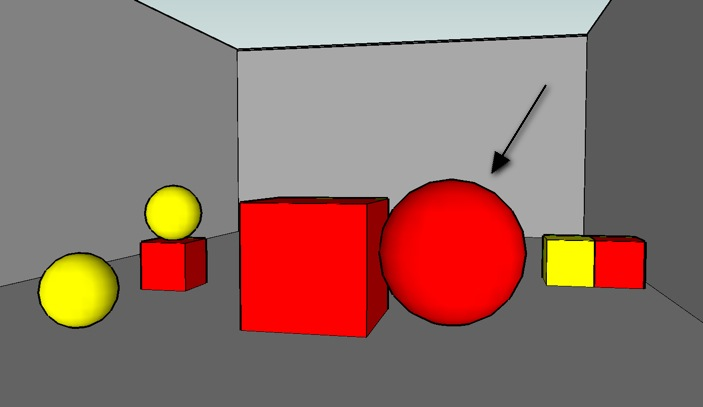
\includegraphics[width=0.6\textwidth]{images/22sinletras.jpg}
\caption{Ejemplo de contexto}
\label{GRE3D7-stimulus}
\end{figure}

Una propiedad es una caracter\'istica propia de un objeto. Por ejemplo en el Contexto \ref{GRE3D7-stimulus} el objeto se\~nalado con la flecha tiene la propiedad {\it color} con valor {\it rojo}. Por simplicidad, en el resto de la tesis vamos a decir ``tiene propiedad {\it rojo}'', cuando queremos decir que el objeto tiene la propiedad color con valor rojo. Una relaci\'on caracteriza a un objeto describiendo caracter\'isticas de otro u otros objetos.\\

%Cuando la ER no es relacional solo contiene propiedades del objeto mismo. Ej.: color, tama\~no. Note que quiz\'as el tama\~no sea con respecto a los dem\'as objetos ``la m\'as peque\~na'', pero al no incluir una descripci\'on de otro objeto no la llamamos relacional.\\
De acuerdo a las propiedades o relaciones que una expresi\'on referencial (ER) incluya, se clasifican en distintos tipos: relacional o no relacional (tambi\'en llamada proposicional), m\'inima, sobreespecificada, o subespecificada. A continuaci\'on describimos cada uno de estos tipos.\\

% en cuyo caso es una expresi\'on que no es referencial, la incluimos en nuestras propiedades porque nos va a ser \'util la definici\'on en el Cap\'itulo \ref{sec:corpus}.\\
Una ER {\it proposicional} o no relacional, incluye s\'olo propiedades intr\'insecas del objeto target. Por ejemplo en el Contexto \ref{GRE3D7-stimulus}: ``La pelota roja''. Las caracter\'isticas de ser pelota, ser roja son propias del objeto identificado.\\

Una ER es {\it relacional}, cuando adem\'as de ser proposicional, contiene relaciones con otros objetos, entonces la ER incluye las ERs de los otros objetos.  Por ejemplo en el Contexto \ref{GRE3D7-stimulus}: ``La pelota que esta a la derecha del cubo grande'', ``a la derecha de'' es una relaci\'on que necesita describir otro objeto adem\'as del target, en este caso ``el cubo grande''.\\

Se dice que una ER es {\it minimal}, cuando incluye la m\'inima cantidad de propiedades con las cuales el objeto puede ser distinguido en el contexto dado. Notar que puede haber muchas expresiones minimales. Por ejemplo en el Contexto \ref{GRE3D7-stimulus} ``La pelota roja'' es una ER minimal, como as\'i tambi\'en lo es ``La pelota grande'', ya que ambas tienen 2 propiedades, y 2 es la m\'inima cantidad de propiedades que puede tener una ER de ese objeto, para distinguirlo en ese contexto.\\

Cuando la ER contiene m\'as informaci\'on de la m\'inima necesaria para distinguirlo de los dem\'as objetos en el contexto dado, se dice que la ER es {\it sobreespecificada}. Por ejemplo: ``La pelota roja grande'' en el Contexto \ref{GRE3D7-stimulus}.\\

Una expresi\'on es {\it subespecificada} cuando no alcanza a ser una ER, ya que no se puede distinguir al objeto target de todos los objetos en el contexto. Por ejemplo: ``La pelota'' en el Contexto \ref{GRE3D7-stimulus} no alcanza para distinguir el objeto apuntado por la flecha, ya que hay otras 2 pelotas. En estos casos se debe dar otra expresi\'on o corregir la anterior agregando m\'as propiedades o relaciones. Una expresi\'on subespecificada identifica a un conjunto, no a un objeto \'unico.

\section{La tarea de generaci\'on autom\'atica de expresiones referenciales}

La generaci\'on autom\'atica de expresiones referenciales (GER), es la tarea de definir cuales pasos se deben seguir para conseguir una ER de un objeto espec\'ifico, en un contexto dado. Estos pasos definen un algoritmo de GER. \\

Los algoritmos se pueden diferenciar por la cantidad y forma de los par\'ametros que toman como input, es decir el modo en que toman por ejemplo el contexto para el cual se espera que den una expresi\'on referencial. \\

En todos los casos, la computadora necesita tener un conjunto de propiedades/relaciones para cada objeto y poder identificarlos, para ello vamos a etiquetar a los objetos con $e_1$, $e_2$, etc. como se muestra en la Figura \ref{GRE3D7-stimulus-conLetras}. En la imagen tambi\'en podemos ver que el objeto se\~nalado con la flecha es $e_5$, es el objeto target, para el cual queremos generar autom\'aticamente una expresi\'on referencial.

\begin{figure}[ht]
\centering
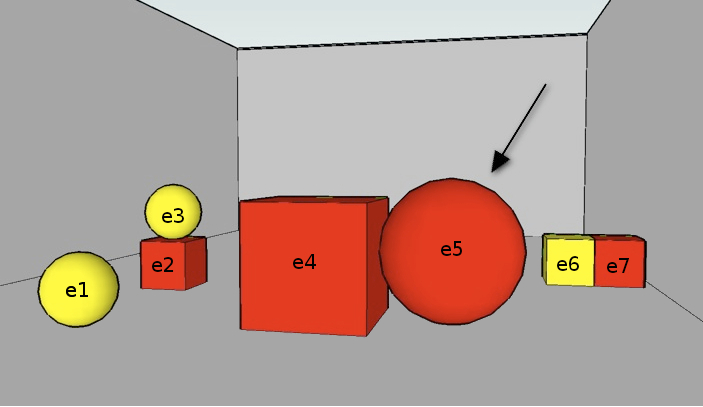
\includegraphics[width=0.6\textwidth]{images/22.jpg}
\caption{Ejemplo de contexto con objetos etiquetados}
\label{GRE3D7-stimulus-conLetras}
\end{figure}

A continuaci\'on daremos 2 ejemplos de diferentes maneras de modelar el contexto que toman como input, uno para el algoritmo Graph y otro para algoritmo de Bisimulaci\'on.\\

%El contexto que toma como input el algoritmo GRAPH \cite{graph08} el cual explicaremos en la Secci\'on \ref{graph}, para el Contexto \ref{GRE3D7-stimulus}, es un grafo dirigido y etiquetado como se muestra en Figura \ref{grafo-GRE3D7-stimulus}, el cual contiene la informaci\'on de las propiedades y relaciones de los objetos, por ejemplo podemos ver que el objeto target que es el $e_5$, tiene propiedades large, red, ball y una flecha con la etiqueta rightof $e_4$, y $e_4$ tiene propiedades large, red, cube, y una flecha hacia $e_5$ con etiqueta leftof.\\

El contexto que toma como input el algoritmo Graph \cite{graph08} el cual explicaremos en la Secci\'on \ref{graph}, para el Contexto \ref{GRE3D7-stimulus}, es un grafo dirigido y etiquetado como se muestra en Figura \ref{grafo-GRE3D7-stimulus}, el cual contiene la informaci\'on de las propiedades y relaciones de los objetos, por ejemplo podemos ver que el objeto $e_5$, tiene propiedades grande, rojo, pelota y una flecha con la etiqueta a-la-derecha-de hacia $e_4$, y $e_4$ tiene propiedades grande, rojo, cubo, y una flecha hacia $e_5$ con etiqueta a-la-izquierda-de.\\

\begin{figure}[ht]
\centering
\begin{tikzpicture}
  [
    n/.style={circle,fill,draw,inner sep=3pt,node distance=2cm},
    aArrow/.style={->, >=stealth, semithick, shorten <= 1pt, shorten >= 1pt},
  ]
 \node[n,label=above:$e_1$,label=below:{
    \relsize{-2}$\begin{array}{c}
      \nSmall\\[-3pt] 
      \nYellow \\[-3pt] 
      \nBall\end{array}$}] (a) {};
 \node[n,label=above:$e_2$,label=below:{
    \relsize{-2}$\begin{array}{c}     
      \nSmall\\[-3pt] 
      \nRed\\[-3pt] 
      \nCube\end{array}$}, right of=a] (b) {};
 \node[n,label=below:$e_3$,label=above:{
    \relsize{-2}$\begin{array}{c}
      \nTop\\[-3pt]      
      \nSmall\\[-3pt] 
      \nYellow\\[-3pt] 
      \nBall\end{array}$}, above of=b] (c) {};
 \node[n,label=right:$e_4$,label=left:{
    \relsize{-2}$\begin{array}{c}
      \nLarge\\[-3pt] 
      \nRed\\[-3pt] 
      \nCube\end{array}$}, right of=b] (d) {};
 \node[n,label=left:$e_5$,label=below:{
    \relsize{-2}$\begin{array}{c}
      \nLarge\\[-3pt] 
      \nRed\\[-3pt] 
      \nBall\end{array}$}, right of=d] (e) {};
 \node[n,label=right:$e_6$,label=left:{
    \relsize{-2}$\begin{array}{c}
      \nSmall\\[-3pt] 
      \nYellow\\[-3pt] 
      \nCube\end{array}$}, right of=e] (f) {};
 \node[n,label=left:$e_7$,label=below:{
    \relsize{-2}$\begin{array}{c}
      \nSmall\\[-3pt]
      \nRed\\[-3pt] 
      \nCube\end{array}$},  right of=f] (g) {};
 \draw [aArrow,bend right=40] (b) to node[auto,swap]{\relsize{-3}$\nBelow$} (c);
 \draw [aArrow,bend right=40] (c) to node[auto,swap]{\relsize{-3}$\nOntop$} (b);
 \draw [aArrow,bend right=40] (d) to node[auto,swap]{\relsize{-3}$\nLeftof$} (e);
 \draw [aArrow,bend right=40] (e) to node[auto,swap]{\relsize{-3}$\nRightof$} (d);
 \draw [aArrow,bend right=40] (f) to node[auto,swap]{\relsize{-3}$\nLeftof$} (g);
 \draw [aArrow,bend right=40] (g) to node[auto,swap]{\relsize{-3}$\nRightof$} (f);
 \draw[dotted] (-0.5,-1.1) rectangle (10.5,3.1);

 \end{tikzpicture}
\caption{Grafo del contexto \ref{GRE3D7-stimulus}}
\label{grafo-GRE3D7-stimulus}
\end{figure}

Para el mismo Contexto \ref{GRE3D7-stimulus-conLetras}, el input del algoritmo de Bisimulaci\'on el cual explicaremos en Secci\'on \ref{bisimulacion}, es un archivo con formato XML \footnote{XML, siglas en ingl\'es de eXtensible Markup Language ('lenguaje de marcas extensible'), es un lenguaje de marcas desarrollado por el World Wide Web Consortium (W3C) utilizado para almacenar datos en forma legible.} con la misma informaci\'on del Contexto \ref{input-bisimulacion}. En este caso se representan las propiedades como relaciones a un objeto ficticio, terminal {\it c}, creado para modelar propiedades y relaciones, como relaciones, como veremos luego esto va a servir para dar prioridad a las relaciones en algunos casos. En el XML podemos ver que todos los objetos tienen ``id'' que es el identificador, salvo el objeto target $e_5$ el cual tiene {\it refer-to} en vez de {\it id}. Con la etiqueta ``rel'', identificamos las relaciones y con la etiqueta ``to'' con que objeto esta relacionado. El target tiene relaciones con c (grande, rojo, pelota) y con $e_4$ a-la-derecha-de.  
%\'Este tiene las relaciones con c (large, red, ball) y con $e_4$ rightof.  
\textcolor{blue}{aca tengo problemas en verbatim para escribir la enie de pequeino}
\label{input-bisimulacion}

%\include{xml}

\begin{verbatim}
<?xml version="1.0"?>
<problem id="e1">c
  <individual id="e1">
    <related rel="pequeno" to="c" />
    <related rel="amarillo" to="c" />
    <related rel="pelota" to="c" />
  </individual>
  ...
  <individual id="e4">
    <related rel="cubo" to="c" />
    <related rel="rojo" to="c" />
    <related rel="grande" to="c" />
    <related rel="a-la-izquierda-de" to="e5" />
  </individual>
  <individual refer-to="e5">
    <related rel="grande" to="c"/>
    <related rel="pelota" to="c" />
    <related rel="rojo" to="c" />
    <related rel="a-la-derecha-de" to="e4" />
  </individual>
  ...
  <individual id="c">
    <related rel="terminal" to="c" />
  </individual> 
</problem>
\end{verbatim}
%\label{input-bisimulacion}
%\begin{verbatim}
%<?xml version="1.0"?>
%<problem id="e1">c
  %<individual id="e1">
    %<related rel="small" to="c" />
    %<related rel="yellow" to="c" />
    %<related rel="ball" to="c" />
  %</individual>
  %...
  %<individual id="e4">
    %<related rel="cube" to="c" />
    %<related rel="red" to="c" />
    %<related rel="large" to="c" />
    %<related rel="left-of" to="e5" />
  %</individual>
  %<individual refer-to="e5">
    %<related rel="large" to="c"/>
    %<related rel="ball" to="c" />
    %<related rel="red" to="c" />
    %<related rel="right-of" to="e4" />
  %</individual>
  %...
  %<individual id="c">
    %<related rel="terminal" to="c" />
  %</individual> 
%</problem>
%\end{verbatim}
%Saque para que no quede tan largo
%<individual id="e6">
    %<related rel="small" to="c" />
    %<related rel="cube" to="c" />
    %<related rel="yellow" to="c" />
    %<related rel="left-of" to="e7" />
  %</individual>
  %<individual id="e7">
    %<related rel="small" to="c" />
    %<related rel="cube" to="c" />
    %<related rel="red" to="c" />
    %<related rel="right-of" to="e6" />
  %</individual>

%<individual id="e2">
%    <related rel="cube" to="c" />
%    <related rel="red" to="c" />
%    <related rel="small" to="c" />
%    <related rel="bellow" to="e3" />
%  </individual>
%  <individual id="e3">
%    <related rel="ball" to="c" />
%    <related rel="yellow" to="c" />
%    <related rel="small" to="c" />
%    <related rel="on-top" to="e2" />
%  </individual>
Los algoritmos tambi\'en se pueden diferenciar por la clase de ER que pueden generar, a continuaci\'on explicaremos los distintos tipos de algoritmos de GER. 

\section{Tipos de algoritmos de GER}

Un algoritmo para la generaci\'on autom\'atica de expresiones referenciales  puede ser: determin\'{i}stico o no-determin\'{i}stico, relacional o proposicional, incluir negaciones o no, identificar plurales o s\'olo singulares,
 %usar disyunciones y conjunciones, o s\'olo conjunciones, 
generar ER sobreespecificadas o minimales.  A continuaci\'on se describen cada uno de esos tipos.\\

Un algoritmo es {\it determin\'{i}stico} si dado un input (un contexto y un objeto target), da siempre la misma ER de salida. En cambio un algoritmo es {\it no-determin\'{i}stico} si es posible que d\'e distintas salidas para el mismo input, en distintas ejecuciones. En general las personas generan expresiones referenciales de forma no determin\'istica, por lo tanto los algoritmos no determin\'isticos simulan el comportamiento de distintas personas, o incluso el de la misma persona en distintos momentos. Por ejemplo ser\'ia no determin\'istico si para el Contexto \ref{GRE3D7-stimulus-conLetras} una vez da ``La pelota roja'' y en otra ejecuci\'on ``La pelota grande''.\\

Un algoritmo es {\it proposicional}, cuando las ER que genera contienen solo atributos del target, es decir no contiene relaciones con otros atributos ni ER de otros objetos.  Por ejemplo para el Contexto \ref{GRE3D7-stimulus-conLetras} una vez da ``La pelota roja''.\\

Un algoritmo es {\it relacional} si adem\'as de generar ER proposicionales genera ER relacionales, en cuyo caso adem\'as de generar las relaciones correspondientes deber\'a generar ERs para el o los objetos relacionados. Por ejemplo para el Contexto \ref{GRE3D7-stimulus-conLetras} la ER ``La pelota roja a la derecha del cubo grande''. En este caso ``el cubo grande'' es una expresi\'on referencial que se tuvo que dar como consecuencia de incluir la relaci\'on ``a la derecha de''.\\

En algunos contextos cuando el target es el \'unico que no tiene una propiedad por ejemplo, ser\'ia \'util un algoritmo que incluya {\it negaciones}. Por ejemplo para el Contexto \ref{GRE3D7-stimulus-conLetras}, ``La \'unica pelota que no es peque\~na''.\\

Un algoritmo puede generar ER para {\it plurales}, es decir dar ER para varios targets en el contexto considerado. Por ejemplo para el Contexto \ref{plurales}, ``Los objetos grandes''. En este caso el target no es \'unico, sino un conjunto de objetos. \\

\begin{figure}[ht]
\centering
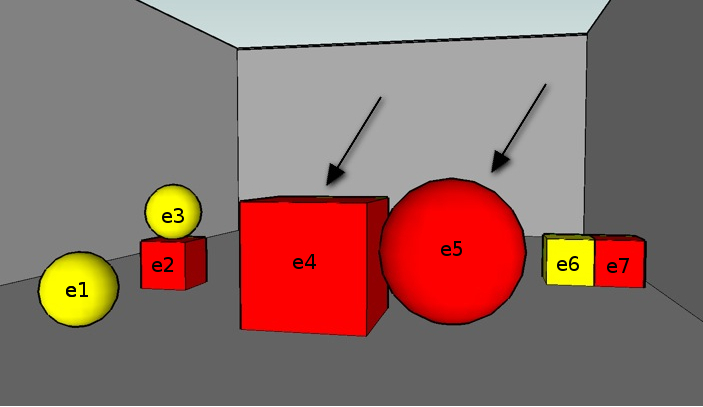
\includegraphics[width=0.6\textwidth]{images/22-plural.jpg}
\caption{Ejemplo de contexto con 2 targets}
\label{plurales}
\end{figure}
%esto lo saque porque confunde aca... me parece que todavia no hay que hablar de esto, es muy de logica
%Los algoritmos tambi\'en se pueden diferenciar en los conectores que permiten si usan conjunciones, disyunciones o ambas.\\

Un algoritmo que genera ER {\it minimales}, es un algoritmo que da ER que contienen la m\'inima cantidad de propiedades o relaciones que se necesitan para distinguir al target.  Por ejemplo para el Contexto \ref{GRE3D7-stimulus-conLetras} ``La pelota grande''.\\

La {\it sobreespecificaci\'on} es la caracter\'istica de dar m\'as atributos o relaciones de las necesarias para identificar al objeto target. Por ejemplo para el Contexto \ref{GRE3D7-stimulus-conLetras} la ER ``La pelota roja, grande que esta a la derecha del cubo rojo grande'' es una ER sobreespecificada.\\

%no se si dejar esto...
%Un algoritmo que hace backtraking, es el que luego de incluir una propiedad o relaci\'on puede deshacer esa inclusi\'on volviendo a un estado anterior, es decir, decidir no incluirla.\\

\section{Algoritmos importantes en el \'area}
%interesante...
%https://www.abdn.ac.uk/ncs/departments/computing-science/tunabibl-495.php

En esta secci\'on vamos a hablar de los algoritmos de generaci\'on autom\'atica de expresiones referenciales, empezando por el algoritmo Full Brevity, el algoritmo de heur\'istica Greedy, siguiendo con el algoritmo Incremental, Graph, algoritmo Relacional y por \'ultimo Bisimulaci\'on.  \\

%http://citeseerx.ist.psu.edu/viewdoc/download?doi=10.1.1.227.8284&rep=rep1&type=pdf

%REG can be traced back to the earliest days of Natural Language Processing; Winograd
%(1972)  (Section  8.3.3,  Naming  Objects  and  Events),  for  example,  sketches  a  primitive
%“incremental” REG algorithm, used in his SHRDLU program. In the 1980s, researchers
%such as Appelt and Kronfeld set themselves the ambitious task of modelling the human
%capacity for producing and understanding referring expressions in programs such as
%KAMP and BERTRAND (Appelt 1985; Appelt and Kronfeld 1987; Kronfeld 1990). They
%argued that referring expressions should be studied as part of a larger speech act. KAMP
%(Appelt  1985),  for  example,  was  conceived  as  a  general  utterance  planning  system,
%building  on  Cohen  and  Levesque’s  (1985)  formal  speech  act  theory.

%REG  task  is  now  defined  by  Dale  and  Reiter  (1995)  through  what  may  be
%called identification of the target: given a target (or referent) object r 2 D , find a set of attribute–value  pairs L
%whose  conjunction  is  true  of  the  target  but  not  of  any  of  the
%distractors (i.e., D

%Full  Brevity  and  Greedy  Heuristic.
El algoritmo {\it Full Brevity} \cite{Dale:1989:CUR:981623.981632} genera la descripci\'on m\'as corta que identifica al target. Para hacerlo, 
busca si hay una propiedad del target que no sea propiedad de ning\'un distractor. Si no hay chequea todas las posibles combinaciones de 2 propiedades, si no la hay, busca de a 3 y as\'i sucesivamente.\\

El problema es que encontrar la descripci\'on m\'as corta es de alta complejidad, se observ\'o que las personas dan expresiones que no son minimales, esto fue confirmado por estudios psycoling\"uisticos (\cite{Olson1970LangAndThought};  \cite{Sonnenschein1984}; \cite{Pechmann1989}; \cite{Engelhardt2006}).\\

Una aproximaci\'on a Full Brevity es el algoritmo de heur\'istica {\it Greedy}, el cual iterativamente selecciona la propiedad que elimina m\'as distractores y argumentan que la propiedad seleccionada tiene el m\'as alto poder discriminativo en esa etapa. Como resultado no siempre genera expresiones referenciales m\'inimas.\\

%which  iteratively  selects  the  property  which  rules  out  most  of  the  distractors
%not  previously  ruled  out,  incrementally  augmenting  the  description  based  on  what
%property has most discriminatory power at each stage (as a result, it does not always
%generate  descriptions  of  minimal  size). 
El algoritmo de heur\'istica Greedy es m\'as eficiente que el Full Brevity, pero pronto fue superado por el algoritmo {\it Incremental} y sus sucesores \cite{C92-1038}; \cite{Dale95computationalinterpretations}. El algoritmo Incremental fue y sigue siendo uno de los algoritmos m\'as importantes del \'area, lo explicamos a continuaci\'on. 
% The  Greedy  Heuristic  algorithm  is  a  more
%efficient  algorithm  than  the  Full  Brevity  one,  but  it  was  soon  eclipsed  by  another
%algorithm    which  turned  out  to  be  the
%most influential algorithm of the pre-2000 era. It is this later algorithm that came to be
%known as``the'' Incremental Algorithm (IA).

%\subsection{GREEDY}

%El algoritmo GREEDY de Dale~\cite{dale89} busca sobre todo el conjunto de propiedades del target y elije el subconjunto m\'as chico posible que identifica un\'{i}vocamente al objeto target entre los distractores en la escena considerada como se muestra en el siguiente algoritmo.\\

%\begin{figure}[ht]
%\begin{center}
%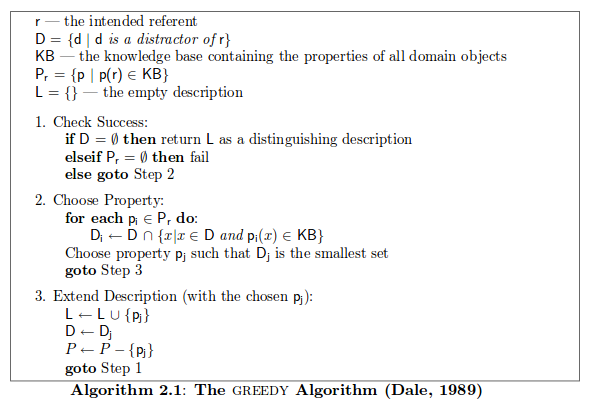
\includegraphics[width=8.5cm]{figures/greedy.png}\\[0pt]
%\caption{Interface del experimento}
%\label{fig-greedy}
%\end{center}
%\end{figure}

%r - el objeto target\\
%D = \{d|d es un distractor de r\}\\
%KB - la base de conocimiento que contiene las propiedades de todos los objetos\\
%$P_{r}$ = $\{p|p(r) \in KB\}$\\
%L = $\{\}$ - la descripci\'on vac\'{i}a\\
%\\
%1. Chequea \'exito:\\
%    \textbf{if} D = $\emptyset$ \textbf{then} return L como una ER que distingue al target r
%    \textbf{elseif} $P_{r}$ = $\emptyset$ \textbf{then} fail
%    
%\textbf{else goto} Paso 2 \\
%\\
%2. Elegir Propiedad:
% \textbf{for each} $p_{i}$ $\in$ $P_{r}$ \textbf{do}:
%    $D_{i}$ $\leftarrow$ D$\cap$ \{x|x $\in$ D and $p_{i}$ (x) $\in$ KB\}
%    Elegir la propiedad $p_{j}$ tal que $D_{j}$ es el conjunto m\'as chico (es decir la que elimina m\'as distractores) \textbf{goto} Paso 3\\
%\\    
%3. Agregar $p_{j}$ a la descripci\'on actual\\
%L $\leftarrow$ L $\cup$ \{$p_{j}$\}\\
%D $\leftarrow$ $D_{j}$\\
%P $\leftarrow$ P -\{$p_{j}$\}\\
%\textbf{goto} Paso 1\\



%%Dado un dominio D que contiene un target referente r y un conjunto de distractores, una base de conocimiento KB que contiene las propiedades de los objetos.
%%Un conjunto de propiedades verdaderas para r, y una descripcion L inicialmente vac\'{i}a.

%Este algoritmo es de orden NP-complete

\subsection{Incremental}

%A continuaci\'on se describe el algoritmo Incremental de Dale \& Reiter el cual esta basado en el algoritmo GREEDY (el cual hac\'ia una b\'usqueda exaustiva y eleg\'ia la propiedad que m\'as distractores eliminaba en cada paso) pero \'este reduce la complejidad del algoritmo Greedy cambiando que en vez de chequear cual propiedad es la que elimina m\'as distractores, eligiendo la que sigue en la lista de propiedades ordenada seg\'un preferencia y que elimina al menos un distractor. Este algoritmo es de orden polinomial. Este algoritmo produce expresiones referenciales que pueden estar sobreespecificadas.\\

\textcolor{blue}{error entorno matematico, pero no entiendo porque, y no puedo hacer que diga algoritmo en vez de algorithm}

%\begin{figure}
\small
\begin{center}
%\centering
\begin{algorithm}[H]

\dontprintsemicolon

\captionsetup[algorithm]{name=Algoritmo}
\caption{Incremental\label{algo:incremental}}
%\caption{Incremental}\label{algo:incremental}
\KwIn{\footnotesize \{r, D, Pref\} r es el target, D es el dominio, Pref lista de preferencia de propiedades ordenadas}
\KwOut{\footnotesize L  - Descripci\'on de salida}

$\ L \leftarrow \emptyset $ \tcp*[f]{\footnotesize Inicialmente es vac\'io}\\
$\ C \leftarrow D - \{r\} $ \tcp*[f]{\footnotesize C es el conjunto de todos los objetos menos r }\\


\For{\em $A_{i} \in Pref$ }{
	$V = Value(r,A_{i})$ \tcp*[f]{\footnotesize V es el valor de la propiedad $A_{i}$ para r }\\
	\If(\tcp*[f]{\footnotesize Si elimina alg\'un distractor}){\em $C \cap RulesOut(\[A_{i}\],V) \neq \emptyset $}
	{
    $\ L \leftarrow L \cup \{A_{i},V\} $  \tcp*[f]{\footnotesize Agrega la propiedad $A_{i}$ a L }\\
    $\ C \leftarrow C - RulesOut(\[A_{i}\],V) $  \tcp*[f]{\footnotesize Actualiza C sacando los objetos que no tienen V en $A_{i}$} 
    }
    \If(\tcp*[f]{\footnotesize Si no quedan distractores}){\em $C = \emptyset $}
	  {
     Return L  
    }
  }
Return Fallo
\end{algorithm}
\end{center}
%\end{figure}



Como podemos ver en \ref{algo:incremental} el input de este algoritmo es el objeto target que queremos identificar {\it r}, D, el dominio, y Pref una lista ordenada de preferencia de propiedades.\\
En {\it Paso 1} se asigna a L la descripci\'on vac\'{i}a, al finalizar la ejecuci\'on, L tendr\'a el conjunto de propiedades con los cuales identificaremos a r, es decir una expresi\'on referencial de r. 
Se le asigna a C el conjunto de distractores de r (todos los objetos menos r), en {\it Paso 2}.\\

La idea del algoritmo es ir eliminando distractores, por eso, en el {\it Paso 3} recorre las propiedades de r. En {\it Paso 4} le asigna a V el valor que tiene el target para la propiedad $A_{i}$

$RulesOut(A_{i},V)$ devuelve el conjunto de objetos que tienen diferente valor para la propiedad $A_{i}$ que el que tiene el objeto target.

Si hay objetos en C que tengan diferente valor de $A_{i}$ que el target, se agrega la propiedad a la descripci\'on actual L en {\it Paso 6}, y se actualiza $C$ sacando los objetos que no tienen V en $A_{i}$. 

Luego en {\it Paso 8} si C es $\emptyset$ (si no hay m\'as distractores) devolvemos L, como el conjunto de propiedades que identifican a r.

Vamos a ejemplificar la corrida del algoritmo con el ejemplo de Contexto \ref{GRE3D7-stimulus-conLetras}, y supongamos que la lista ordenada de propiedades es esta [ tipo, color, tama\~no ]. D inicialmente es \{$e_{1}$,$e_{2}$,$e_{3}$,$e_{4}$,$e_{5}$,$e_{6}$,$e_{7}$\}
Al iniciar a L le asigna $\emptyset$ y a C \{$e_{1}$,$e_{2}$,$e_{3}$,$e_{4}$,$e_{6}$,$e_{7}$\}, luego comienza a recorrer la lista de propiedades, la primer propiedad es ``tipo'', el valor del target para tipo es {\it pelota}, entonces en {\it Paso 6}, pregunta si hay objetos que tengan tipo con valor distinto de pelota, y hay, ellos son \{$e_{2}$,$e_{4}$,$e_{6}$,$e_{7}$\}, entonces le asigna a C \{$e_{1}$,$e_{3}$\}, es decir solo las pelotas. En {\it Paso 10} pregunta si C es vac\'io, no lo es, por lo tanto continua con la siguiente propiedad, en este caso ``color'', el valor de color para el target es {\it rojo}, agrega {\it rojo} a L, y actualiza C con $\emptyset$ porque tanto $e_{1}$ como $e_{3}$ son amarillos, en {\it Paso 10} pregunta si C es vac\'io, y si lo es, por lo tanto devuelve \{pelota, rojo\}.


%Intuitivamente, si la primer propiedad tipo y el valor de tipo para el target es ``pelota'', nos quedamos con todos los objetos pelota.\\

%\textcolor{blue}{Un poco mas de historia, no se a donde poner...Theune and Krahmer proposed an extension that allows the generation of subsequent reference with the ia taking into account the discourse salience of the target referent (Krahmer and Theune, 1998; Theune, 2000; Krahmer and Theune, 2002), and a second one which allows the ia to produce referring expressions that
%contain binary relations to other objects (Theune, 2000; Krahmer and Theune, 2002). I will return to their relational extension in Section 2.3. Theune and Krahmer's approach works by assigning a salience score to all objects according to the
%focus/topic distinction by Hajicova (1993) and Centering Theory (Grosz et al., 1995). They alter the success criterion of the algorithm and only let it stop when here is no distractor left that is as or more salient than the target referent.
%Not all properties are the same. The qualitative diferences that exist between diferent properties were first discussed in the
%reg literature by van Deemter (2000, 2006). He pointed out that the appropriateness of
%vague orgradable properties such as small and large is dependent on the context in which they are used, while,
%for example, the colour of an object is absolute. Consider two descriptions in a domain of animals... (van Deemter, 2002), van Deemter considered the ia's logical completeness in terms of the Boolean operators of negation and disjunction. He extended it to
%be able to generate referring expressions that contain negated properties, such as Example (2.3), and descriptions of sets of objects, such as Example (2.4), or even (2.5), which contains a logical disjunction of properties. His algorithm proceeds
%in stages, trying longer and longer disjunctions of properties, if atomic properties
%and shorter disjunctions did not suffice to distinguish the target set.. he work on reference to sets was taken further by Gatt and van Deemter (2005, 2006), who have presented the most mature algorithms in this space to
%date. They used a similar procedure to the ia in that their algorithms are based
%on incremental processing of a preference order of properties. Their algorithms
%add a lot of complex machinery to the basic procedure to ensure that properties
%are chosen in a way that maximises coherence within the set of objects described
%by the referring expressions. For example, their approach will attempt to use
%properties of the same type for all the referents of a set. So, it would produce
%descriptions such as Examples 
Luego se propusieron extensiones del algoritmo Incremental, por ejemplo 
Theune y Krahmer propusieron una extensi\'on que permite la generaci\'on de referencia teniendo en cuenta la prominencia discurso del target (\cite{Krahmer:2010:EMN:1880370}; \cite{krahmer-theune:2002a};), y un segundo algoritmo que permite producir expresiones referenciales que contienen relaciones con otros objetos. El enfoque Theune y de Krahmer funciona asignando una puntuaci\'on de relevancia a todos los objetos de acuerdo con el enfoque / tema distinci\'on por \cite{hajicova-1993} y la teor\'ia de centrado \cite{Grosz:1995:CFM:211190.211198}. Alteran el criterio de \'exito del algoritmo y s\'olo permiten que se detenga cuando hay un distractor que es tanto o m\'as relevante que el target.
No todas las propiedades tienen la misma relevancia. Las diferencias cualitativas que existen entre diferentes propiedades se discutieron por primera vez en la literatura GER por van Deemter (2000, 2006). Se\~nal\'o que la conveniencia de otras propiedades sobre las
propiedades vagas como peque\~no y grande dependen del contexto en el que se utilizan, mientras que, por ejemplo, el color de un objeto es absoluta. 
%Considere dos descripciones de un dominio de los animales ... (van Deemter, 2002), van Deemter considera integridad l\'ogica del ia en t\'erminos de los operadores booleanos de negaci\'on y disyunci\'on. \'el la extendi\'o a
%ser capaz de generar expresiones referenciales que contienen propiedades, tales como Ejemplo (2.3) negado, y las descripciones de conjuntos de objetos, tales como Ejemplo (2.4), o incluso (2,5), que contiene una disyunci\'on l\'ogica de propiedades. Sus algoritmo procede
%en etapas, tratando m\'as y disyunciones m\'as largos de propiedades, si las propiedades at\'omicas
%y disyunciones m\'as cortos no son suficientes para distinguir el conjunto target .. que funciona en referencia a conjuntos fue tomada adem\'as por Gatt y van Deemter (2005, 2006), que han presentado los algoritmos m\'as maduros a la fecha. Utilizaron un procedimiento similar al de las otras cosas en que sus algoritmos se basan en el procesamiento incremental de un orden de preferencia de las propiedades. Sus algoritmos agregan una gran cantidad de maquinaria compleja para el procedimiento b\'asico para asegurar que las propiedades
%se eligen de manera que maximiza la coherencia dentro del conjunto de objetos descritos por las expresiones referenciales. Por ejemplo, su enfoque intentar\'a utilizar propiedades del mismo tipo para todos los referentes de un conjunto. As\'i, ser\'ia producir
%descripciones tales como ejemplos
%(2.6) or (2.7) rather than Example (2.8) or.. 


%Theune y Krahmer propusieron una extensi\'on que permite la generaci\'on de referencia con la subsiguiente ia teniendo en cuenta la prominencia discurso del referente objetivo (Krahmer y Theune, 1998; Theune, 2000; Krahmer y Theune, 2002), y un segundo uno que permite la IA para producir expresiones referenciales que contener relaciones binarias a otros objetos (Theune, 2000; Krahmer y Theune, 2002). Voy a volver a su extensi\'on relacional en la Secci\'on 2.3. Enfoque Theune y de Krahmer funciona asignando una puntuaci\'on de relevancia a todos los objetos de acuerdo con la enfoque / tema distinci\'on por Hajicova (1993) y el centrado Theory (Grosz et al., 1995). Alteran el criterio de \'exito del algoritmo y s\'olo permiten que se detenga cuando aqu\'i hay izquierda distractor que es tan o m\'as relevante que el referente de destino.
%No todas las propiedades son las mismas. Las Diferencias cualitativas que existen entre diferentes propiedades se discutieron por primera vez en la literatura reg por van Deemter (2000, 2006). Se\~nal\'o que la conveniencia de propiedades orgradable vagos como peque\~nos y grandes depende del contexto en el que se utilizan, mientras que, Por ejemplo, el color de un objeto es absoluta. Considere dos descripciones de un dominio de los animales ... (van Deemter, 2002), van Deemter considera integridad l\'ogica del ia en t\'erminos de los operadores booleanos de negaci\'on y disyunci\'on. \'el la extendi\'o a ser capaz de generar expresiones que se refieren que contienen propiedades, tales como Ejemplo (2.3) negado, y las descripciones de conjuntos de objetos, tales como Ejemplo (2.4), o incluso (2,5), que contiene una disyunci\'on l\'ogica de propiedades. Sus algoritmo procede en etapas, tratando m\'as y disyunciones m\'as largos de propiedades, si las propiedades at\'omicas y disyunciones m\'as cortos no son suficientes para distinguir el conjunto de destino .. que funciona en referencia a conjuntos fue tomada adem\'as por Gatt y van Deemter (2005, 2006), que han presentado los algoritmos m\'as maduros en este espacio para la fecha. Utilizaron un procedimiento similar al de las otras cosas en que sus algoritmos se basan en el procesamiento incremental de un orden de preferencia de las propiedades. Sus algoritmos agregar una gran cantidad de maquinaria compleja para el procedimiento b\'asico para asegurar que las propiedades se eligen de manera que maximiza la coherencia dentro del conjunto de objetos descritos por las expresiones que se refieren. Por ejemplo, su enfoque intentar\'a utilizar propiedades del mismo tipo para todos los referentes de un conjunto. As\'i, ser\'ia producir Ejemplos descripciones tales como (2,6) o (2,7) en lugar de Ejemplo (2.8) o ..


\subsection{Algoritmo de b\'usqueda en Grafo}
\label{graph}
%Un grafo es un conjunto de objetos llamados v\'ertices o nodos unidos por enlaces llamadas aristas o arcos, que permiten representar relaciones binarias entre elementos de un conjunto. \\

Un grafo G es un par ordenado $G=(V,E)$, donde:
\begin{itemize}
   \item V es un conjunto de v\'ertices o nodos, y
    \item E es un conjunto de aristas o arcos, que relacionan estos nodos.

%\item Se llama orden del grafo G a su n\'umero de v\'ertices, $|V|$.

%\item El grado de un v\'ertice o nodo $v \in V$ es igual al n\'umero de arcos que lo tienen como extremo.

%\item Un bucle es una arista que relaciona al mismo nodo; es decir, una arista donde el nodo inicial y el nodo final coinciden.

%\item Dos o m\'as aristas son paralelas si relacionan el mismo par de v\'ertices.

%\item Un grafo puede ser dirigido o no, etiquetado o no.
\end{itemize}
%T\'{i}picamente, un grafo se representa gr\'aficamente como un conjunto de puntos (v\'ertices o nodos) unidos por l\'{i}neas (aristas).

Los grafos han sido muy estudiados, pr\'acticamente cualquier problema puede ser expresado como un problema de grafos, y aplicar algoritmos de b\'usqueda ya estudiados.

El algoritmo Graph de \cite{Krahmer:2003} propone ver la obtenci\'on de expresiones referenciales como un problema de grafos, el contexto que incluye al target y los distractores es representado como un grafo. \\

Cada objeto de la escena se modela como un v\'ertice en el grafo. Las propiedades at\'omicas como color, tipo o tama\~no se representan como un bucle en el correspondiente nodo. Est\'an etiquetados con los nombres de las propiedades y los valores que el objeto en cuesti\'on tiene para estas propiedades. \\

Las relaciones binarias entre objetos, por ejemplo abajo-de, arriba-de se modelan como aristas entre los nodos correspondientes.\\

%La base de conocimiento que incluye al target ahora esta expresada como los v\'ertices, las aristas y las etiquetas del grafo.\\

%Krahmer et al.'s (2003) reformularon la tarea de seleccionar las propiedades y relaciones que contendr\'a una expresi\'on referencial como un problema de teor\'ia de grafos.

Para generar una descripci\'on distintiva, el algoritmo busca un subgrafo del grafo original que identifica al target un\'{i}vocamente, le llama grafo distintivo.\\% (distinguishing graph).\\

Comenzando con el subgrafo que contiene un solo v\'ertice, que representa al target, se realiza una b\'usqueda exhaustiva, pero comenzando a lo ancho. Utiliza una heur\'{i}stica basada en el costo (costo de incluir propiedades, relaciones) para podar el espacio de b\'usqueda. Y da el grafo de menor costo. \\


%esto no se entiende nada
%Informalmente, un subgrafo refiere al target si y s\'olo si puede ser
%`Colocado sobre el gr\'afico de dominio de tal manera que el v\'ertice que representa subgrafo
%del objeto target se puede `coloca sobre 'el v\'ertice del objetivo en el gr\'afico de dominio,
%y cada uno de los bordes marcados en el subgrafo puede ser `coloca sobre 'un correspondiente
%borde en el gr\'afico de dominio con la misma etiqueta y el mismo sentido. Por otra parte,
%un subgrafo distingue al target un\'ivocamente si y s\'olo si se puede `colocarlo sobre grafo original' y es exactamente el
%v\'ertice target. La noci\'on informal de un gr\'afico que se coloca sobre otro corresponde al concepto te\'orico matem\'atico de isomorfismo de grafos.

En teor\'{i}a de grafos, un isomorfismo entre dos grafos G y H es una biyecci\'on f entre los conjuntos de sus v\'ertices $f:V(G) \rightarrow V(H)$ que preserva la relaci\'on de adyacencia. Es decir, cualquier par de v\'ertices u y v de G son adyacentes si y solo si lo son sus im\'agenes, $f(u)$ y $f(v)$, en H.\\

%\textcolor{blue}{aca quiero poner un ejemplo que muestre una imagen y el modelo como grafo}

La funci\'on de costo esta definida sobre las aristas y v\'ertices del grafo dominio. El costo de un subgrafo se define como la suma sobre todas las aristas y v\'ertices que contiene el grafo.\\
El algoritmo de b\'usqueda garantiza encontrar el subgrafo de menor costo que representa al target.\\

La funci\'on de costo es usada para podar las ramas del \'arbol de b\'usqueda cuando estas se hacen m\'as costosas que el grafo de menor costo encontrado hasta el momento. Esta funci\'on hace que se prefieran propiedades sobre otras que tienen mayor costo.

\textcolor{blue}{aca quiero agregar ejemplo, no me gusta como quedo esta parte}


\subsection{Bisimulaci\'on}
\label{bisimulacion}

%Este algoritmo fue propuesto por %\cite{}

La idea es transformar el problema de GER al problema de computar una f\'ormula de l\'ogicas para la descripci\'on (DL) cuya extensi\'on sea el elemento target (o los elementos targets, en el caso de querer dar una ER para plurales aprovechando que una f\'ormula describe un conjunto que puede contener m\'as de un elemento).\\

A continuaci\'on daremos una introducci\'on a las l\'ogicas para la descripci\'on \alc y \el.\\

\emph{F\'ormulas} (o \emph{conceptos}) $\varphi$ de $\alc$ son generadas por la siguiente gram\'atica:
$$
\varphi,\varphi' ::= \top \mid p \mid \neg \varphi \mid \varphi \sqcap \varphi'
\mid \exists R. \varphi
$$
donde $p$ es el conjunto de los s\'imbolos proposicionales \prop y $R$ es el de los s\'imbolos relacionales \rel. $\el$ es la parte sin negaci\'on de $\alc$.\\

Las f\'ormulas de ambos $\alc$ y $\el$ son interpretadas en modelos relacionales de primer orden $\gM = (\Delta,\interp{\cdot})$ donde
$\Delta$ es un conjunto no vac\'io y $\interp{\cdot}$ es una funci\'on de interpretaci\'on tal que:
$$
\begin{array}{ccl}
\interp{p} & \subseteq & \Delta  \mbox{ para $p \in \prop$}\\
\interp{R} & \subseteq & \Delta \times \Delta  \mbox{ para $R \in \rel$}\\
\interp{\neg \varphi} & = & \Delta - \interp{\varphi}\\
\interp{\varphi \sqcap \varphi'} & = & \interp{\varphi} \cap \interp{\varphi'}\\
\interp{\exists R.\varphi} & = & \{i \mid \mbox{para alg\'un } i', (i,i') \in \interp{R}\\
& & \mbox{ e } i' \in \interp{\varphi} \}.\\
\end{array}
$$

\begin{figure}[ht]
\begin{center}
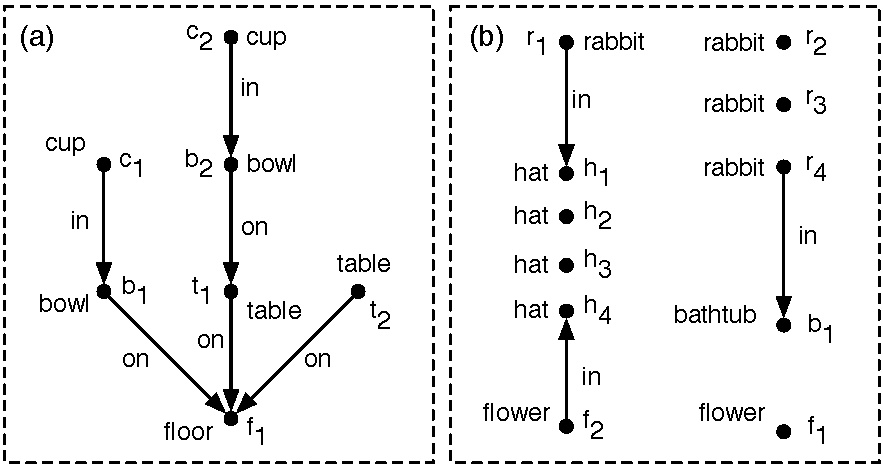
\includegraphics[width=8.5cm]{figures/pic-dale-haddock.pdf}\\[0pt]
\caption{}
\label{fig:dale-haddock}
\end{center}
\end{figure}


Cada f\'ormula de una descripci\'on l\'ogica denota un conjunto de objetos del dominio; por lo tanto podemos usar tales f\'ormulas para describir conjuntos. Por ejemplo en el modelo de la Figura.~\ref{fig:dale-haddock}b, la f\'ormula
$\mathsf{flower}$ denota el conjunto $\{f_1,f_2\}$; La f\'ormula
$\mathsf{flower} \sqcap \exists \mathsf{in}.\mathsf{hat}$ denota
$\{f_2\}$; y la f\'ormula $\mathsf{flower} \sqcap \neg
\exists \mathsf{in}.\mathsf{hat}$ denota $\{f_1\}$.\\

\textcolor{blue}{no se si dejar este ejemplo, o cambiarlo por uno es espa\~nol}

Hay muchas otras l\'ogicas de descripci\'on (DL) en la literatura por ejemplo 

$\mathcal{CL}$ (\el\ sin el cuantificador existencial, es decir solo conjunciones at\'omicas); $\mathcal{PL}$ (\alc\ l\'ogica propocisional); y
$\mathcal{ELU}_{(\neg)}$ (\el\ m\'as disjunci\'on y negaci\'on at\'omica).\\

Usaremos una noci\'on de preservaci\'on de f\'ormulas que llamaremos
\emph{similaridad}. Para cualquier DL $\gL$, diremos que un individual $i$ es \emph{\gL-similar} a $i'$ en un modelo dado $\gM$
si para cualquier f\'ormula $\varphi \in \gL$ tal que $i \in
\interp{\varphi}$, tambi\'en tenemos que $i' \in \interp{\varphi}$.\\
Equivalentemente, no hay $\gL$-f\'ormula que se mantenga para $i$ pero no para
$i'$.  Diremos que el \emph{\gL-conjunto de similaridad} de alg\'un individual
$i$ es el conjunto de todos los individuales a los cuales $i$ es \gL-similar.\\

Notar que la similaridad no es necesariamente una relaci\'on sim\'etrica: Por ejemplo:$f_1$ es \el-similar a $f_2$ en
Figura~\ref{fig:dale-haddock}b, pero $f_2$ no es \el-similar a $f_1$
(satisface la f\'ormula $\exists \mathsf{in}.\mathsf{hat}$ y $f_1$
no la satisface).  De todas maneras, \alc-similaridad es una relaci\'on sim\'etrica porque
el languaje contiene negaci\'on; y en consecuencia, $f_1$ no es \alc-similar
a $f_2$ porque este tampoco satisface $\neg \exists
\mathsf{in}.\mathsf{hat}$.  Porque \alc\ es m\'as expresivo que \el,
esto es, para alg\'un individual $a$ es posible ser \el-similar pero
no \alc-similar a alg\'un individual $b$, pero no viceversa.\\



%\textcolor{blue}{SACAR ESTO... poner quizas en la introduccion o en primer capitulo. Las ER que involucran relaciones han recibido m\'as atenci\'on recientemente;
%especialmente en el contexto de las expresiones referenciales espaciales en generaci\'on (por ejemplo,~\cite{kelleher06:increm}), donde es particularmente natural utilizar expresiones que implican relaciones espaciales, tales como ``la pelota en la parte superior del cubo''. Sin embargo, el algoritmo cl\'asico por~\cite{dale91:gener} ha demostrado ser incapaz de generar ER satisfactorias en la pr\'actica (v\'ease el an\'alisis sobre el~\emph{cabinet corpus} en~\cite{viethen06:_algor_for_gener_refer_expres}). Adem\'as, el Dale y Haddock algoritmo y muchos de sus sucesores (tales como~\cite{kelleher06:increm}) son vulnerables a el problema de la \emph{regresi\'on infinita}, donde el algoritmo entra en un bucle infinito, saltando hacia atr\'as y hacia adelante entre las descripciones para dos individuos emparentados, como en `` el libro sobre la mesa que soporta una libro sobre la mesa \ldots ''}

%REs involving relations have received increasing attention recently;
%especially in the context of spatial referring expressions in situated
%generation (e.g., \cite{kelleher06:increm}),
%where it is particularly natural to use expressions involving spatial
%relations such as ``the ball on top of the cube.''  However, the
%classical algorithm
%by~\cite{dale91:gener} was shown to be
%unable to generate satisfying REs in practice (see the analysis over
%the \emph{cabinet corpus}
%in~\cite{viethen06:_algor_for_gener_refer_expres}).  Furthermore, the
%Dale and Haddock algorithm and many of its successors (such
%as~\cite{kelleher06:increm}) are vulnerable to
%the problem of \emph{infinite regress}, where the algorithm enters an
%infinite loop, jumping back and forth between descriptions for two
%related individuals, as in ``the book on the table which supports a
%book on the table \ldots''

%\cite{arec2:2008:Areces,arec:usin11} have proposed low complexity
%algorithms for the generation of relational REs
%%(including references to sets) 
%that eliminate the risk of infinite regression.  These algorithms are
%based on variations of the partition refinement algorithms
%of~\cite{paig:thre87}.  The information provided by a given scene
%is interpreted as a relational model whose objects are classified into
%sets that fit the same description.  This classification is
%successively \emph{refined} till the target is the only element
%fitting the description of its class.  The existence of an ER depends
%on the information available in the input scene, and on the expressive
%power of the formal language used to describe elements of the
%different classes in the refinement.


\cite{arec2:2008:Areces,arec:usin11} han propuesto algoritmos de baja complejidad
 para la generaci\'on de ER relacionales que eliminan el riesgo de regresi\'on infinita. Estos algoritmos son
basados en variaciones de los algoritmos de refinamiento de particiones
de~\cite{paig:thre87}. La informaci\'on proporcionada por una escena dada
se interpreta como un modelo relacional cuyos objetos se clasifican en
conjuntos que se adaptan a la misma descripci\'on. Esta clasificaci\'on es
sucesivamente \emph{refinada} hasta que el target es el \'unico elemento
en la clase. La existencia de una ER depende
de la informaci\'on disponible en la escena de entrada, y del poder expresivo
del lenguaje formal utilizado para describir los elementos de las
diferentes clases en el refinamiento.\\

%Refinement
%algorithms %presented in~\cite{arec2:2008:Areces,arec:usin11}
%effectively compute REs for all individuals in the domain, at the same
%time. The algorithms always terminate returning a formula of the
%formal language chosen that uniquely describes the target (if the
%formal language is expressive enough to identify the target in the
%input model).
%\cite{arec2:2008:Areces}
%show that the refinement algorithm using the description language \el  is capable of generating 67\% of 
%the relational REs in the~\cite{viethen06:_algor_for_gener_refer_expres} dataset, when all possible orders of the relations in the domain are considered. This is in sharp contrast with the analysis 
%done in~\cite{viethen06:_algor_for_gener_refer_expres} over the cabinet corpus, of algorithms based in Dale and Reiter's original proposal.    

%Los algoritmos de refinamiento
% presenta en~\cite{arec 2:2008:Areces, arec:usin11}
%calculan efectivamente ER para todos los objetos en el dominio, al mismo
%tiempo. Los algoritmos siempre terminan devolviendo una f\'ormula del
%lenguaje formal elegido que describe un\'{i}vocamente el target (si el
%lenguaje formal es suficientemente expresivo para identificar el target en el
%modelo de entrada).\\

%Refinement algorithms for GER are based on the following basic idea:
%given a scene $S$, the objects appearing in $S$ are successively
%classified according to their properties into finer and finer
%classes. A description (in some formal language $\mathcal{L}$) of each
%class is computed every time a class is refined. The procedure always
%stops when the set of classes stabilizes, i.e., no further refinement
%is possible with the information available in the scene\footnote{Of
%  course, if we are only interested in a referring expression for a
%  given target we can stop the procedure as soon as the target is the
%  only element of some of the classes.}.  If the target element is in
%a singleton class, then the formal description of that class is a
%referring expression; otherwise the target cannot be unequivocally
%described (in 


%It is clear that a scene can be encoded in different ways as a
%relational model (for example in \ref{figure22}, we could argue that
%$e_1$ is also \emph{leftof} $e_2$, not considered because they are no
%touching). The algorithm assumes that these issues have been resolved
%and that the model encodes a suitable representation of the scene we
%want to describe.  Moreover, we will assume that all relations are
%\emph{binary}.  We will not consider relations of arity greater than
%two (relations of higher arity can be encoded as binary relations via
%reification, if necessary).

\begin{figure}[ht]
%\begin{minipage}[b]{0.45\linewidth}
%\centering
\begin{center}
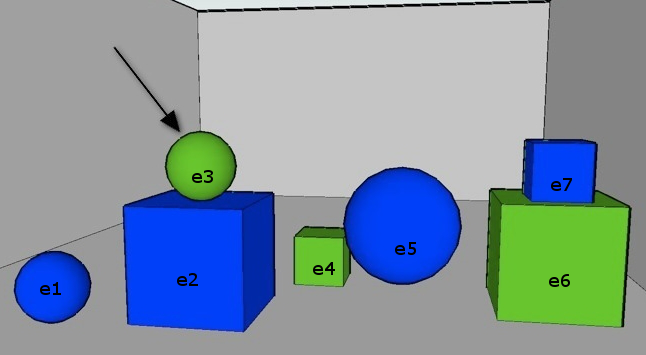
\includegraphics[width=0.5\textwidth]{images/3b.png}
\caption{Contexto de ejemplo}\label{GRE3D7-stimulus-cap2}
%\end{minipage}
\end{center}
\end{figure}

%\textcolor{blue}{hice mas grande la figura porque no se leian, como la pase a espaniol y se me fue al pie, no se porque}
%\hspace*{-0.35cm}
\begin{figure}[ht]
\begin{center}
%\begin{minipage}[b]{0.5\linewidth}
%\centering
\begin{tikzpicture}
  [
    n/.style={circle,fill,draw,inner sep=3pt,node distance=2.6cm},
    aArrow/.style={->, >=stealth, semithick, shorten <= 2pt, shorten >= 2pt},
  ]
 \node[n,label=above:$e_1$,label=below:{
    \relsize{-1}$\begin{array}{c}
      \nLeft\\[-2pt]
      \nSmall\\[-2pt] 
      \nBlue \\[-2pt] 
      \nBall\end{array}$}] (a) {};

 \node[n,label=above:$e_2$,label=below:{
    \relsize{-1}$\begin{array}{c}
      \nLeft\\[-2pt]
      \nBig\\[-2pt] 
      \nBlue\\[-2pt] 
      \nCube\end{array}$}, right of=a] (b) {};

 \node[n,label=below:$e_3$,label=above:{
    \relsize{-1}$\begin{array}{c}
      \nTop\\[-2pt]
      \nLeft\\[-2pt]
      \nSmall\\[-2pt] 
      \nGreen\\[-2pt] 
      \nBall\end{array}$}, above of=b] (c) {};

 \node[n,label=above:$e_4$,label=below:{
    \relsize{-1}$\begin{array}{c}
      \nSmall\\[-2pt] 
      \nGreen\\[-2pt] 
      \nCube\end{array}$}, right of=b] (d) {};

 \node[n,label=above:$e_5$,label=below:{
    \relsize{-1}$\begin{array}{c}
      \nBig\\[-2pt] 
      \nBlue\\[-2pt] 
      \nBall\end{array}$}, right of=d] (e) {};

 \node[n,label=above:$e_6$,label=below:{
    \relsize{-1}$\begin{array}{c}
      \nBig\\[-2pt] 
      \nGreen\\[-2pt] 
      \nCube\end{array}$}, right of=e] (f) {};

 \node[n,label=below:$e_7$,label=above:{
    \relsize{-1}$\begin{array}{c}
      \nTop\\[-2pt]
      \nSmall\\[-2pt] 
      \nBlue\\[-2pt] 
      \nCube\end{array}$}, above of=f] (g) {};

 \draw [aArrow,bend right=90] (b) to node[auto,swap]{\relsize{-1}$\nBelow$} (c);
 \draw [aArrow,bend right=90] (c) to node[auto,swap]{\relsize{-1}$\nOntop$} (b);

 \draw [aArrow,bend right=70] (d) to node[auto,swap]{\relsize{-1}$\nLeftof$} (e);
 \draw [aArrow,bend right=70] (e) to node[auto,swap]{\relsize{-1}$\nRightof$} (d);

 \draw [aArrow,bend right=90] (f) to node[auto,swap]{\relsize{-1}$\nBelow$} (g);
 \draw [aArrow,bend right=90] (g) to node[auto,swap]{\relsize{-1}$\nOntop$} (f);

 \draw[dotted] (-.6,-1.4) rectangle (12.5,4.5);

 \end{tikzpicture}
\caption{Modelo relacional del Contexto \ref{GRE3D7-stimulus-cap2}}
\label{GRE3D7-stimulus-graph}
%\end{minipage}
\end{center}
\end{figure}

Algoritmos de refinamiento para GER se basan en la siguiente idea b\'asica:
dada una escena $S$, los objetos que aparecen en $S$ son sucesivamente
clasificados de acuerdo con sus propiedades en clases m\'as y m\'as finas. 
Una descripci\'on (en alg\'un lenguaje formal de $\mathcal{L}$) de cada
clase se calcula cada vez que una clase es refinada. El procedimiento siempre
se detiene cuando el conjunto de clases se estabiliza, es decir, no se puede hacer m\'as refinamiento
con la informaci\'on disponible en la escena \footnote{Por supuesto, si s\'olo estamos interesados en una expresi\'on referencial de un objeto dado, se puede detener el procedimiento en cuanto el objetivo es el
   \'unico elemento de alguna de las clases.}

Si el elemento target est\'a en
una clase singleton, entonces la descripci\'on formal de esa clase es un
expresi\'on referencial; de lo contrario el target no puede ser un\'{i}vocamente
descripto (en $\mathcal{L}$).\\

Est\'a claro que una escena puede ser codificada en diferentes formas como un
modelo relacional (por ejemplo, en \ref{GRE3D7-stimulus-cap2}, podr\'{i}amos argumentar que
$e_1$ es tambi\'en \emph{leftof} $e_2$, pero no lo consideramos porque no se estan 
tocando en la imagen). El algoritmo asume que estas cuestiones se han resuelto y que el modelo codifica una representaci\'on adecuada de la escena que
queremos describir. Por otra parte, vamos a suponer que todas las relaciones son
\emph{binarias}. No vamos a considerar las relaciones de aridad mayor que
dos (relaciones de mayor aridad pueden codificarse como relaciones binarias v\'{i}a
reificaci\'on, si es necesario).\\

%On termination, the algorithm computes what are called the
%$\mathcal{L}$-similarity classes of the input model $\gM$.
%Intuitively, the referring expression ``\textsf{ball}'' and ``\textsf{cube}''  are more specific and then contain more information than $\top$.


Tras la resoluci\'on, el algoritmo calcula lo que se llama la
$\mathcal{L}$ - clases de semejanza del modelo de entrada de $\gM$.\\

%There is many $\mathcal{L}$, we will name $\alc$ and $\el$

%ACA VOY A PONER gramatica para generar... ALC y EL no quedaria bien aca, hay que ver lo agregamos antes o no hace falta
%In what follows, we use formulas of the $\el$ description logic
%language
En lo que sigue, se utilizan f\'ormulas de la descripci\'on de la l\'ogica $\el$
~\cite{baad:desc03} para describir las clases de refinamiendo
\footnote{N\'otese, sin embargo, que el lenguaje formal particular usado es
   independiente del algoritmo principal, y diferentes funciones
  add$_{\mathcal{L}}$($\varphi$,\RE) se pueden utilizar dependiendo
   de la l\'ogica en cuesti\'on.}. como se discuti\'o 
en~\cite{arec2:2008:Areces}, 
este lenguaje es adecuado para describir
RE conjuntivas y relacionales, que son lo que encontramos en los corpus.

  La entrada al algoritmo ser\'a un modelo $\mathcal{M} =
 \tup{\Delta, \interp{\cdot}}$, donde $\Delta$ es el dominio no vac\'io de objetos de la imagen,
 $\interp{\cdot}$ es una funci\'on de interpretaci\'on que asigna a todas las propiedades de la escena su extensi\'on.
 Por ejemplo, la escena mostrada en la Figura~\ref{GRE3D7-stimulus-cap2} podr\'ia ser representada por el modelo
 $\gM=\tup{\Delta,\interp{\cdot}}$ mostrado en la 
 Figura~\ref{GRE3D7-stimulus-graph}; donde+- $\Delta =
 \{e_1,\ldots,e_7\}$, e $\interp{\textsf{red}}$ is $\{e_2, e_4, e_5,
 e_7\}$.

Se llama extensi\'on de una f\'ormula al conjunto de objetos que la hacen v\'alida.

$\top$ es una f\'ormula que representa la descripci\'on m\'as general, cuya
interpretaci\'on incluye todos los elementos del modelo. Se podr\'ia realizar
como la ER con el sustantivo
``\textsf{cosa}''. Decimos que una f\'ormula es
\emph{subsumida} por otras f\'ormulas, cuando su extensi\'on puede ser cubierta por la
union de las extensiones de las otras f\'ormulas. Por ejemplo, en la
Figura~\ref{GRE3D7-stimulus-cap2}, $\top$ es subsumida por ``\textsf{ball}'' y
``\textsf{cube}'', porque $\interp{\top}$ = $\interp{\textsf{ball}}
\cup \interp{\textsf{cube}}$.
%= $\{e_2, e_4, e_6, e_7\}$, it is $\{e_1, e_2, e_3, e_4, e_5, e_6, e_7\}$ = $\{e_1, e_3, e_5\} \cup \{e_2, e_4, e_6, e_7\}$. 
Intuitivamente la f\'ormula ``\textsf{cube}'' o ``\textsf{ball}'' tienen m\'as informaci\'on que $\top$, para cada elemento de $\top$, hay una f\'ormula que d\'a m\'as informaci\'on, digamos ``\textsf{cube}'' es m\'as informativa que ``\textsf{cosa}''.\\

%In the following we will explain an example of execusion of the
%algorithm shown in Figure
%A continuaci\'on vamos a explicar un ejemplo de ejecusi\'on del
%algoritmo mostrado en la Figura~\ref{algoritmoOriginal} considerando la l\'ogica 
%$\el$ como language. Este algoritmo fue presentado en
%~\cite{arec2:2008:Areces}.
%
%\begin{figure}[h!]
%\begin{center}
%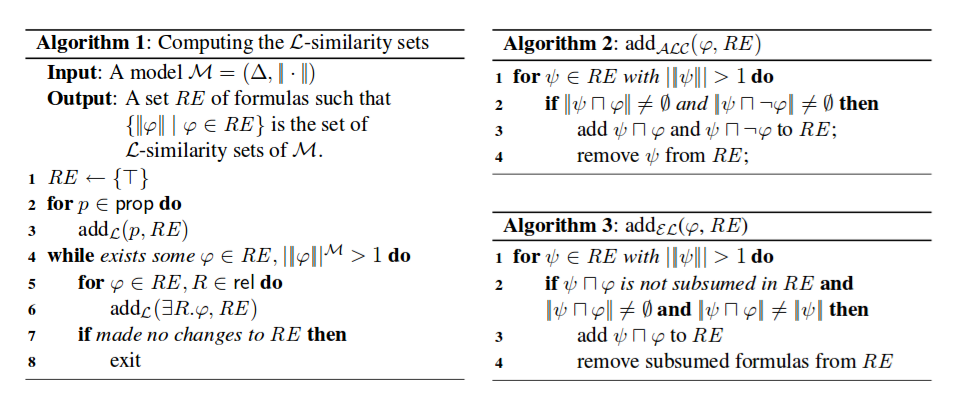
\includegraphics[width=\textwidth]{images/algoritmoOriginal.png}
%\end{center}
%\vspace*{-2em}
%\caption{Algoritmo para GER con l\'ogicas de descripci\'on}
%\label{algoritmoOriginal}
%\end{figure}

%\subsection{Ejemplo de ejecuci\'on}
%
%
%
%\textcolor{blue}{no se si poner aca un ejemplo, si poner el texto y las im\'agenes en otro apendice... o ponerlas mas chiquitas en varias columnas, asi queda feo}\\
%Vamos a ejecutar el algoritmo para la Figura~\ref{GRE3D7-stimulus-cap2},
%el algoritmo comienza con una lista fija de propiedades y relaciones, supongamos que
%esas listas son las siguientes:
%
%propiedades ordenadas (prop): \textsf{ball}, \textsf{cube}, \textsf{red}, \textsf{yellow}, \textsf{small}, \textsf{large}.\\
%relaciones ordenadas (rel): \textsf{leftof}, \textsf{rightof}, \textsf{ontopof}, \textsf{bellowof}.
%
%%\begin{figure}
%%\begin{center}	
%%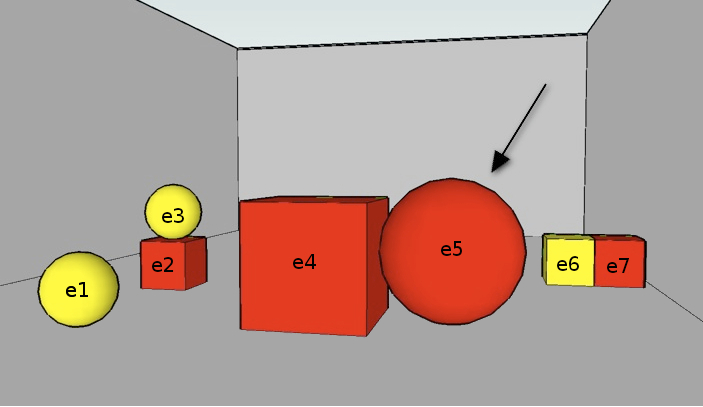
\includegraphics[width=.5\textwidth]{images/22.jpg}
%%\end{center}
%%\vspace*{-1.5em}
%%\caption{Escena 3D de figuras geom\'etricas}\label{figure22}
%%\end{figure}
%
%%\begin{figure}
%%\begin{minipage}[b]{0.6\linewidth}
%%\centering
%%\begin{tikzpicture}
%%  [
%%    n/.style={circle,fill,draw,inner sep=3pt,node distance=1.4cm},
%%    aArrow/.style={->, >=stealth, semithick, shorten <= 2pt, shorten >= 2pt},
%%  ]
%% \node[n,label=above:$e_1$,label=below:{
%%    \relsize{-1}$\begin{array}{c}
%%      \nLeft\\[-2pt]
%%      \nSmall\\[-2pt] 
%%      \nYellow \\[-2pt] 
%%      \nBall\end{array}$}] (a) {};
%
%% \node[n,label=above:$e_2$,label=below:{
%%    \relsize{-1}$\begin{array}{c}
%%      \nLeft\\[-2pt]
%%      \nSmall\\[-2pt] 
%%      \nRed\\[-2pt] 
%%      \nCube\end{array}$}, right of=a] (b) {};
%
%% \node[n,label=below:$e_3$,label=above:{
%%    \relsize{-1}$\begin{array}{c}
%%      \nTop\\[-2pt]
%%      \nLeft\\[-2pt]
%%      \nSmall\\[-2pt] 
%%      \nYellow\\[-2pt] 
%%      \nBall\end{array}$}, above of=b] (c) {};
%
%% \node[n,label=above:$e_4$,label=below:{
%%    \relsize{-1}$\begin{array}{c}
%%      \nBig\\[-2pt] 
%%      \nRed\\[-2pt] 
%%      \nCube\end{array}$}, right of=b] (d) {};
%
%% \node[n,label=above:$e_5$,label=below:{
%%    \relsize{-1}$\begin{array}{c}
%%      \nBig\\[-2pt] 
%%      \nRed\\[-2pt] 
%%      \nBall\end{array}$}, right of=d] (e) {};
%
%% \node[n,label=above:$e_6$,label=below:{
%%    \relsize{-1}$\begin{array}{c}
%%      \nSmall\\[-2pt] 
%%      \nYellow\\[-2pt] 
%%      \nCube\end{array}$}, right of=e] (f) {};
%
%% \node[n,label=above:$e_7$,label=below:{
%%    \relsize{-1}$\begin{array}{c}
%%      \nSmall\\[-2pt] 
%%      \nRed\\[-2pt] 
%%      \nCube\end{array}$}, right of=f] (g) {};
%
%% \draw [aArrow,bend right=90] (b) to node[auto,swap]{\relsize{-1}$\nBelow$} (c);
%% \draw [aArrow,bend right=90] (c) to node[auto,swap]{\relsize{-1}$\nOntop$} (b);
%
%% \draw [aArrow,bend right=30] (d) to node[auto,swap]{\relsize{-1}$\nLeftof$} (e);
%% \draw [aArrow,bend right=30] (e) to node[auto,swap]{\relsize{-1}$\nRightof$} (d);
%
%% \draw [aArrow,bend right=30] (f) to node[auto,swap]{\relsize{-1}$\nLeftof$} (g);
%% \draw [aArrow,bend right=30] (g) to node[auto,swap]{\relsize{-1}$\nRightof$} (f);
%
%% \draw[dotted] (-.4,-1.7) rectangle (7.5,3.3);
%
%% \end{tikzpicture}
%%\caption{La escena como modelo relacional}\label{GRE3D7-stimulus-graph}
%%\end{minipage}
%%\end{figure}
%
%
%El algoritmo siempre termina, y devuelve ER un conjunto de f\'ormulas que describe cada elemento en el dominio (si existe esa f\'ormula). \\
%
%En el comienzo ER=$\{\top\}$ y $\interp{\top}$ = $\{e_1, e_2, e_3, e_4, e_5, e_6, e_7\}$ como se puede ver en la Figura~\ref{fig-modelo}.\\
%
%ACA
%\begin{figure}[ht]
%\begin{minipage}[b]{0.45\linewidth}
%\centering
%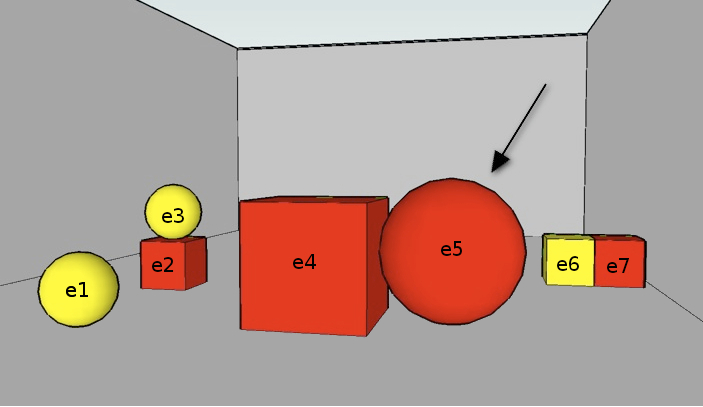
\includegraphics[width=\textwidth]{images/22.jpg}
%\vspace*{1cm}
%%\caption{Input scene}
%\label{GRE3D7-stimulus-22}
%\end{minipage}
%%\hspace*{-0.35cm}
%\begin{minipage}[b]{0.6\linewidth}
%\centering
%%\begin{figure}[ht]
%%\begin{center}
%\frame{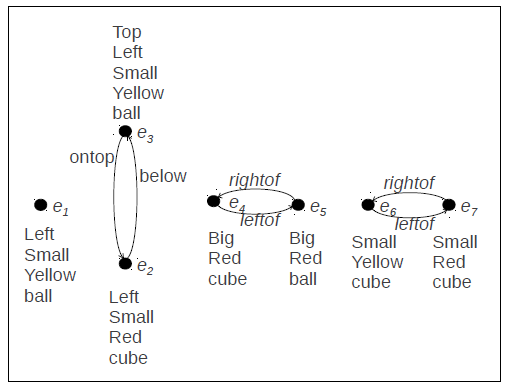
\includegraphics[width=8cm]{images/modelo.png}}\\[0pt]
%\caption{Modelo de la Figura \ref{GRE3D7-stimulus-22}}
%\label{fig-modelo}
%\end{minipage}
%\end{figure}
%El primer bucle del algoritmo es en las propiedades. Para cada propiedad hace add$_\el$ ($\varphi$, RE), las propiedades at\'omicas se muestran en la Figura~\ref{fig-modelo2}.
%
%\begin{figure}[ht]
%\begin{center}
%\frame{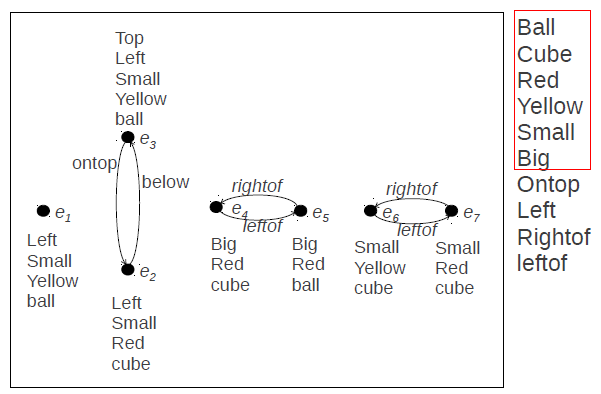
\includegraphics[width=8cm]{images/modelo2.png}}\\[0pt]
%\caption{Propiedades proposicionales en cuadro rojo, las del primer ciclo del algoritmo}
%\label{fig-modelo2}
%\end{center}
%\end{figure}
%
%La f\'ormula $\varphi$ se a\~nadir\'a a ER si su interpretaci\'on tiene al menos un elemento, a continuaci\'on, para cada f\'ormula
 %$\psi$ en ER la conjunci\'on
%$\varphi  \wedge \psi$ no necesita estar subsumida in ER, la $\interp{\varphi \cup \psi}$ no tiene que ser vac\'io, y su interpretaci\'on tiene que ser distinta de $\interp{\psi}$. Luego las f\'ormulas subsumidas se borran.
%
%La primer propiedad es \textsf{ball}, ER = \{$\top$, \textsf{ball}\}, se ven los elementos de ``ball'' en un recuadro en la Figura~\ref{fig-modelo3}.
%
%\begin{figure}[ht]
%\begin{center}
%\frame{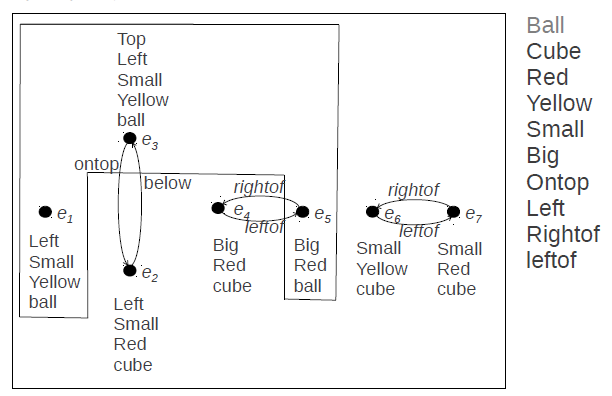
\includegraphics[width=8cm]{images/modelo3.png}}\\[0pt]
%\caption{El cuadro indica cuales son ``ball''}
%\label{fig-modelo3}
%\end{center}
%\end{figure}
%
%La siguiente propiedad es \textsf{cube}, ER = \{$\top$, \textsf{ball}, \textsf{cube}\}, pero ahora la $\interp{\textsf{ball}}$ = $\{e_1, e_3, e_5\}$, $\interp{\textsf{cube}}$ = $\{e_2, e_4, e_6, e_7\}$, quedando las particiones como se muestra en la Figura~\ref{fig-modelo4}
%\begin{figure}[ht]
%\begin{center}
%\frame{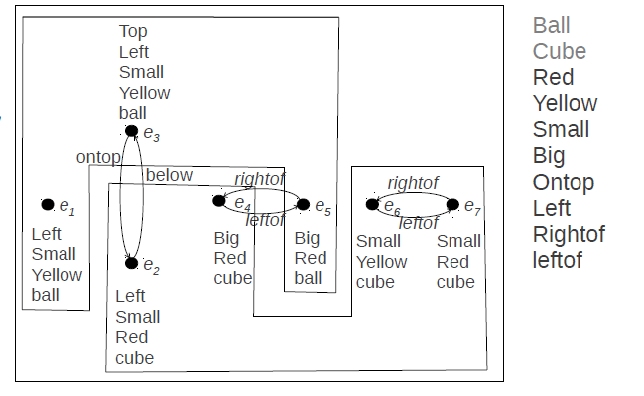
\includegraphics[width=8cm]{images/modelo4.png}}\\[0pt]
%\caption{Cuadros indicando ``ball'' y ``cube''}
%\label{fig-modelo4}
%\end{center}
%\end{figure}
%Ahora podemos borrar $\top$, porque es subsumida (esta cubierta por) las otras dos f\'ormulas. La siguiente propiedad es  \textsf{red}, $\interp{\textsf{red}}$ es: $\{e_2, e_4, e_5, e_7\}$, haciendo la intersecci\'on con la $\interp{.}$ de cada f\'ormula en ER obtenemos, $\{e_5\}$ y $\{e_2, e_4, e_7\}$, ER = $\{\textsf{ball}, \textsf{cube}, \textsf{ball} \wedge \textsf{red}, \textsf{cube} \wedge \textsf{red}\}$, las particiones actuales se pueden ver en la Figura~\ref{fig-modelo9}.
%\begin{figure}[ht]
%\begin{center}
%\frame{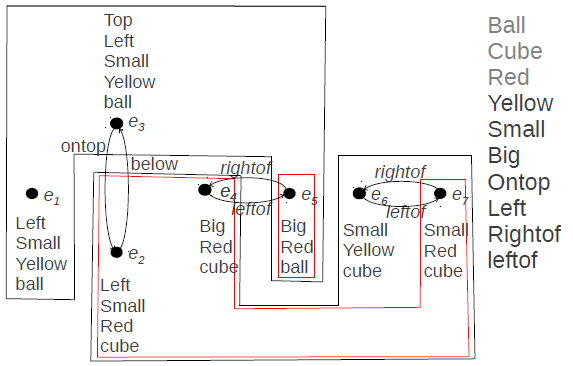
\includegraphics[width=8cm]{images/modelo9.png}}\\[0pt]
%\caption{Cuadros indicando ``ball'', ``cube'' y ``red''}
%\label{fig-modelo9}
%\end{center}
%\end{figure}
%
%Siguiendo con \textsf{yellow}, tenemos, $\interp{\textsf{yellow}}$ = $\{e_1, e_3, e_6\}$ y obtenemos ER = $\{\textsf{ball} \wedge \textsf{yellow}, \textsf{cube} \wedge \textsf{yellow}, \textsf{ball} \wedge \textsf{red}, \textsf{cube} \wedge \textsf{red}\}$. 
%Note que aqu\'i ya borramos la f\'ormula \textsf{ball} porque estaba subsumida, y la f\'ormula \textsf{cube} tambi\'en. Se muestran particiones en Figura~\ref{fig-modelo10}.
%
%\begin{figure}[ht]
%\begin{center}
%\frame{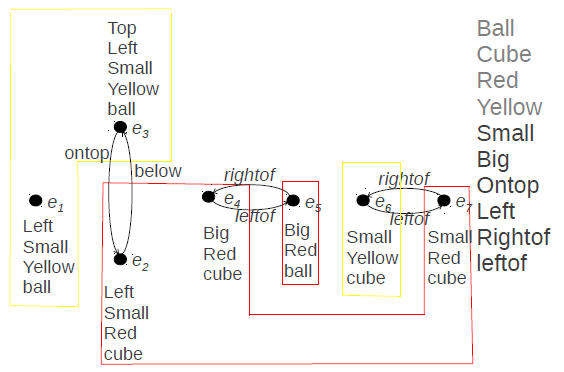
\includegraphics[width=8cm]{images/modelo10.png}}\\[0pt]
%\caption{Cuadros indicando ``ball'', ``cube'', ``red'' y ``yellow''}
%\label{fig-modelo10}
%\end{center}
%\end{figure}
%
%Haciendo lo mismo con \textsf{small} tenemos ER = $\{\textsf{ball} \wedge \textsf{yellow} \wedge \textsf{small}, \textsf{cube} \wedge \textsf{yellow} \wedge \textsf{small}, \textsf{ball} \wedge \textsf{red}, \textsf{cube} \wedge \textsf{red}, \textsf{cube} \wedge \textsf{red} \wedge \textsf{small}\}$, como se puede ver en Figura~\ref{fig-modelo11}.
%\begin{figure}[ht]
%\begin{center}
%\frame{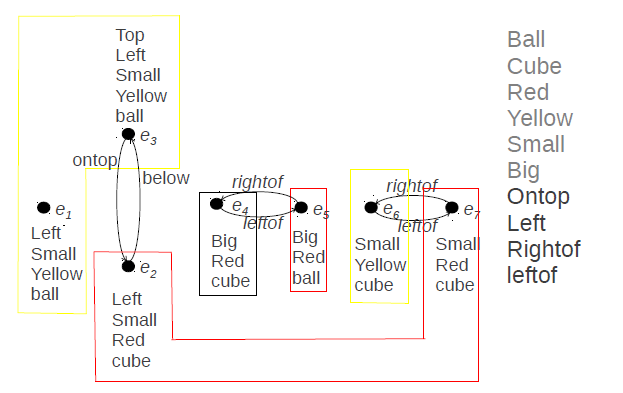
\includegraphics[width=8cm]{images/modelo11.png}}\\[0pt]
%\caption{Cuadros indicando ``ball'', ``cube'', ``red'', ``yellow'', ``small'' y ``large''}
%\label{fig-modelo11}
%\end{center}
%\end{figure}
%
%La siguiente propiedad es \textsf{large} as\'i, tenemos ER = $\{\textsf{ball} \wedge \textsf{yellow} \wedge \textsf{small}, \textsf{cube} \wedge \textsf{yellow} \wedge \textsf{small}, \textsf{ball} \wedge \textsf{red}, \textsf{cube} \wedge \textsf{red} \wedge \textsf{large}, \textsf{cube} \wedge \textsf{red} \wedge \textsf{small}\}$. Aqu\'i no podemos agregar \textsf{large} a la f\'ormula $\textsf{red} \wedge \textsf{cube}$ porque su interpretaci\'on tiene un solo elemento, y la condici\'on dice que es necesario tener m\'as de uno.
%
%Hasta ahora ER = $\{\textsf{ball} \wedge \textsf{yellow} \wedge \textsf{small}, \textsf{cube} \wedge \textsf{yellow} \wedge \textsf{small}, \textsf{ball} \wedge \textsf{red}, \textsf{cube} \wedge \textsf{red} \wedge \textsf{large}, \textsf{cube} \wedge \textsf{red} \wedge \textsf{small}\}$ 
%y tenemos las siguientes extensiones: $\{e_1, e_3\}, \{e_6\}, \{e_5\}, \{e_4\}, \{e_2, e_7\}$ respectivamente. 
%Hay dos f\'ormulas que a\'un pueden ser refinadas, $\textsf{ball} \wedge \textsf{yellow} \wedge \textsf{small}$ y $\textsf{cube} \wedge \textsf{red} \wedge \textsf{small}$ 
%debido a que tienen m\'as de un elemento cada una, por lo que entran en el ciclo, while del algoritmo 1, en la l\'inea 4. Ahora es el turno de las relaciones, la primera de ellas es \textsf{leftof}, para cada f\'ormula $\varphi$ en ER trataremos de hacer add$_\el$ ($\exists \textsf{leftof}.\varphi$, RE). Notar que $\psi$ solo puede ser $\textsf{ball} \wedge \textsf{yellow} \wedge \textsf{small}$ o $\textsf{cube} \wedge \textsf{red} \wedge \textsf{small}$ porque esos son los que su interpretaci\'on tiene m\'as de un elemento. 
%\begin{figure}[ht]
%\begin{center}
%\frame{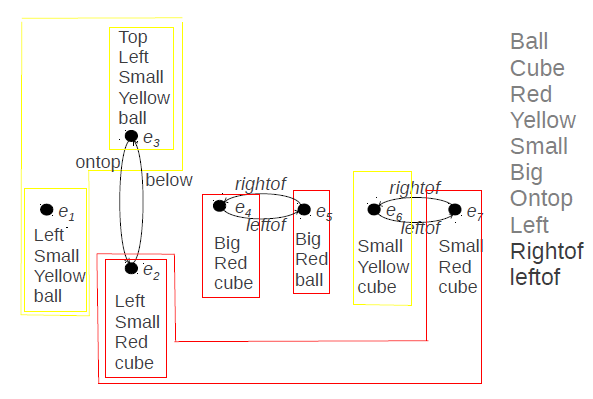
\includegraphics[width=8cm]{images/modelo15.png}}\\[0pt]
%\caption{Cuadros indicando ``ball'', ``cube'', ``red'', ``yellow''...}
%\label{fig-modelo15}
%\end{center}
%\end{figure}
%
%
%No hay
%%because those are the ones that its interpretation have more than one element. There is not 
%$\varphi$ y $\psi$ que puedan ser aplicadas. Continuando con \textsf{rightof} agregamos $\textsf{cube} \wedge \textsf{yellow} \wedge \textsf{small} \wedge \exists \textsf{rightof}. \textsf{cube} \wedge \textsf{red} \wedge \textsf{small}$, y asi con \textsf{topof} agregamos $\textsf{small} \wedge \textsf{red} \wedge \textsf{cube} \wedge \exists \textsf{ontop}. \textsf{small} \wedge \textsf{yellow} \wedge \textsf{ball}$ y el algoritmo termina con ER = $\{\textsf{ball} \wedge \textsf{yellow} \wedge \textsf{small}, \textsf{cube} \wedge \textsf{yellow} \wedge \textsf{small}, \textsf{ball} \wedge \textsf{red}, \textsf{cube} \wedge \textsf{red} \wedge \textsf{large}, \textsf{cube} \wedge \textsf{red} \wedge \textsf{small}, \textsf{cube} \wedge \textsf{yellow} \wedge \textsf{small} \wedge \exists \textsf{rightof}. \textsf{cube} \wedge \textsf{red} \wedge \textsf{small}, \textsf{small} \wedge \textsf{red} \wedge \textsf{cube} \wedge \exists \textsf{ontop}. \textsf{small} \wedge \textsf{yellow} \wedge \textsf{ball}\}$, 
%aqu\'i todos los elementos est\'an en una clase singleton y no se puede hacer ning\'un refinamiento m\'as. 
%%can be applied to $cube \wedge red \wedge small$ but there is no formula which interpretation has more than one element to be apply with this one. The same happen for the other relations, so the algorithm ends.
%%its interpretation is $\{e_7\}$ with $\psi$ is $cube \wedge yellow \wedge small$, the others combinations can't be apply because they don't do true the preconditions. The following relation is rightof, 
%
%%leftof, rightof, ontopof, bellowof
%
%%At this point we already have the target in a singleton set. So the formula for it is ``red and ball'', and also for s6 which formula is ``yellow cube''.\\
%%As we show this algorithm depends of the order of properties and relations.\\
%\begin{figure}[ht]
%\begin{center}
%\frame{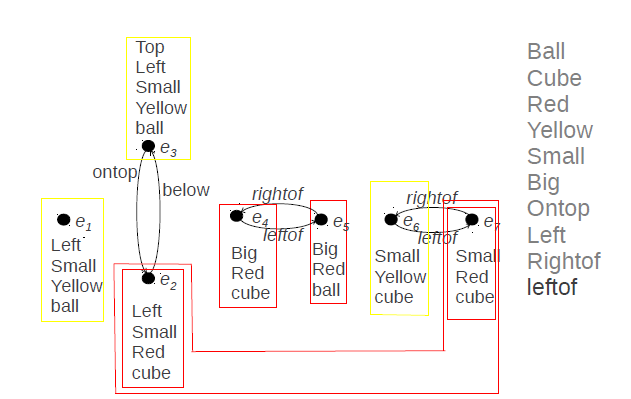
\includegraphics[width=8cm]{images/modelo16.png}}\\[0pt]
%\caption{Cuadros indicando ``ball'', ``cube'', ``red'', ``yellow''...}
%\label{fig-modelo16}
%\end{center}
%\end{figure}
%
%\begin{figure}[ht]
%\begin{center}
%\frame{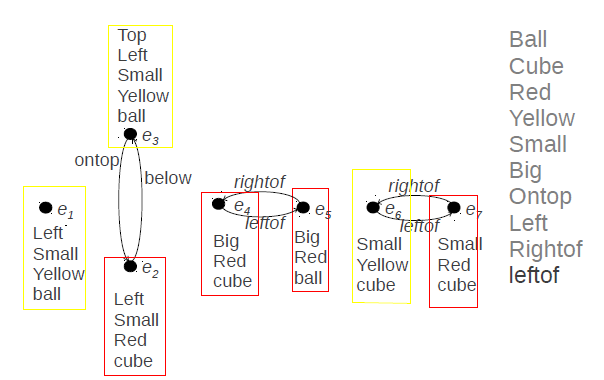
\includegraphics[width=8cm]{images/modelo17.png}}\\[0pt]
%\caption{Cuadros indicando ``ball'', ``cube'', ``red'', ``yellow''...}
%\label{fig-modelo17}
%\end{center}
%\end{figure}
%
%Las expresiones referenciales encontradas son:\\
%
%$\textsf{ball} \wedge \textsf{yellow} \wedge \textsf{small}$ representa $e_1$ \\
%$\textsf{cube} \wedge \textsf{yellow} \wedge \textsf{small}$ representa $e_6$ \\
%$\textsf{ball} \wedge \textsf{red}$ representa $e_5$ \\
%$\textsf{cube} \wedge \textsf{red} \wedge \textsf{large}$ representa $e_4$ \\
%$\textsf{cube} \wedge \textsf{red} \wedge \textsf{small}$ representa $\{e_2,e_7\}$  \\
%$\textsf{cube} \wedge \textsf{yellow} \wedge \textsf{small} \wedge \exists \textsf{rightof}. \textsf{cube} \wedge \textsf{red} \wedge \textsf{small}$ representa $e_6$ \\
%$\textsf{small} \wedge \textsf{red} \wedge \textsf{cube} \wedge \exists \textsf{ontop}. \textsf{small} \wedge \textsf{yellow} \wedge \textsf{ball}$ representa $e_2$ \\
%



\section{Aproximaciones emp\'iricas a la soluci\'on de GER}

\subsection{Corpus existente}
\label{sec:corpus2}
\label{sec:corpusTUNA}

%was the first prominent REG corpus to be made publicly available for research purposes. The corpus was developed in a series of general-purpose controlled experiments, containing 2280 descriptions produced by 60 speakers in two domains (1200 descriptions of furniture items and 1080 descriptions of people's photographs). TUNA does not contain relational descriptions, and it is possibly the only resource of this kind to include situations of reference to sets. The TUNA corpus has been extensively used in a series of shared tasks

TUNA \cite{tuna-corpus} fue el primer corpus prominente para GER disponible p\'ublicamente con fines de investigaci\'on. El corpus fue desarrollado en una serie de experimentos controlados de prop\'osito general, contiene 2.280 descripciones producidas por 60 personas en dos dominios (1.200 expresiones referenciales de im\'agenes de muebles y 1080 expresiones referenciales de fotograf\'ias de personas situadas en una grilla). Se muestran ejemplos de im\'agenes en Figuras \ref{fig-TUNA-furniture} y \ref{fig-TUNA-people}. El corpus TUNA no contiene descripciones relacionales, y es posiblemente el \'unico recurso de este tipo que incluye situaciones de referencia a conjuntos. Este corpus se ha utilizado ampliamente en una serie de desaf\'ios \cite{reg2009}. \\

\begin{figure}
\begin{minipage}[t]{0.5\linewidth}
\centering
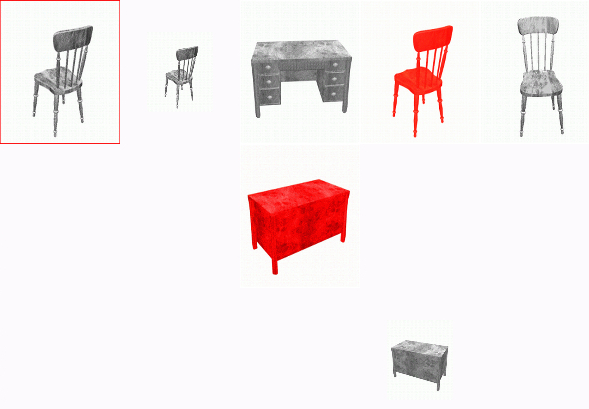
\includegraphics[width=\textwidth]{images/largeGreyChair.jpg}\\[0pt]
\caption{Imagen del TUNA corpus (muebles)}
\label{fig-TUNA-furniture}
\vspace*{.1cm}
\end{minipage}
\hspace*{0cm}
\begin{minipage}[t]{0.5\linewidth}
\centering
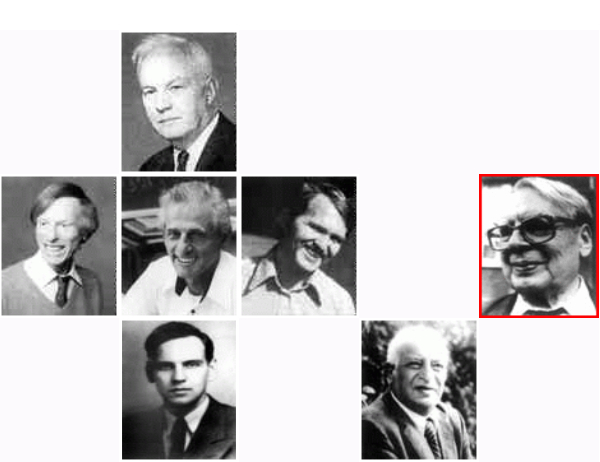
\includegraphics[width=\textwidth]{images/tuna-people.jpg}\\[0pt]
\caption{Imagen del TUNA corpus (personas)}
\label{fig-TUNA-people}
\end{minipage}
\end{figure}


\label{sec:corpusGRE}
%were developed in a series of web-based experiments primarily focussed on the study of relational descriptions. GRE3D3 contains 630 descriptions produced by 63 speakers, and GRE3D7 contains 4480 descriptions produced by 287 speakers, making it the largest of its kind to date. The GRE3D domain consists of simple visual scenes containing only two kinds of objects (boxes and spheres) with limited variation in colour and size. In each scene, there is only one possible spatial relation between target and the nearest landmark. Both corpora contain atomic and relational descriptions.
GRE3D3 y su extensi\'on GRE3D7 \cite{gre3d3,gre3d7} se desarrollaron en una serie de experimentos basados en la web, se centraron principalmente en el estudio de las descripciones relacionales. GRE3D3 contiene 630 descripciones producidas por 63 personas y GRE3D7 contiene 4.480 descripciones producidas por 287 personas, y es el corpus m\'as grande de este tipo hasta la fecha. El dominio del GRE3D3 consta de escenas visuales simples que contienen s\'olo dos tipos de objetos (cubos y esferas) con variaci\'on limitada en color y tama\~no. En cada escena, s\'olo hay una posible relaci\'on espacial entre el target y el landmark m\'as cercano. Ambos corpus contienen descripciones at\'omicas y relacionales. Ejemplo de im\'agenes del GRE3D3 y GRE3D7 se muestran en las Figuras \ref{fig-GRE3D3} y \ref{fig-GRE3D7}.\\
%\begin{minipage}[b]{0.45\linewidth}

\begin{figure}
\begin{minipage}[b]{0.5\linewidth}
\centering
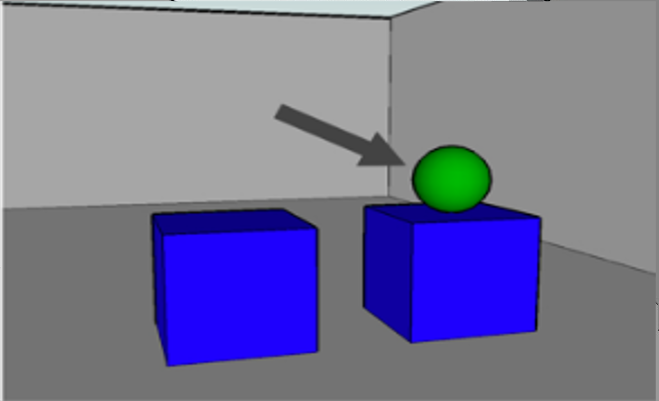
\includegraphics[width=\textwidth]{images/GRE3D3.png}\\[0pt]
\caption{Imagen del GRE3D3}
\label{fig-GRE3D3}
\vspace*{-0.7cm}
\end{minipage}
\hspace*{0cm}
\begin{minipage}[b]{0.5\linewidth}
\centering
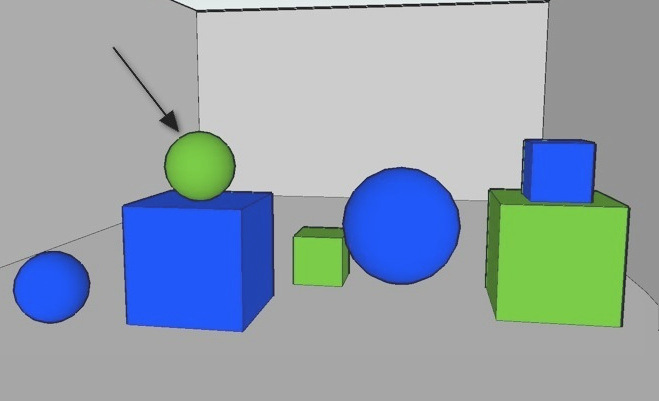
\includegraphics[width=\textwidth]{images/3.jpg}\\[0pt]
\caption{Imagen del GRE3D7}
\label{fig-GRE3D7}
\end{minipage}
\end{figure}

%\vspace*{3cm}

\label{sec:corpusSTARS}
%and its extension Stars2 were collected for the study of referential overspecification (particularly in the case of relational descriptions). Stars was developed in a pilot web-based experiment, containing 704 descriptions produced by 64 speakers.  The more comprehensive Stars2 data set was produced in dialogue situations involving subject pairs, and it contains 884 descriptions produced by 56 speakers. Both domains make use of simple visual scenes containing up to four object types (e.g., stars, boxes, cones and spheres) with limited variation in colour and size. Differently from other REG corpora, however, Stars/2 includes a considerable number of complex situations of reference involving up to three objects, as in `the box near the sphere, next to the cone'.http://ppgsi.each.usp.br/arquivos/RelTec/PPgSI-002_2014.pdf y http://ppgsi.each.usp.br/arquivos/RelTec/PPgSI-001_2015.pdf
Stars \cite{stars-mutual-disamb} y su extensi\'on Stars2 se colectaron para el estudio de la sobre-especificaci\'on (particularmente en el caso de las descripciones relacionales). Stars se desarroll\'o en un experimento piloto basado en la web, contiene 704 descripciones producidas por 64 personas. El conjunto de datos Stars2 es m\'as completo y se obtuvo de situaciones de di\'alogo que implicaban a dos personas, contiene 884 descripciones producidas por 56 participantes. Ambos dominios hacen uso de escenas visuales simples que contienen tres tipos de objetos (por ejemplo para Stars, estrellas, cuadrados y c\'irculos y para Stars2 cubos, conos y esferas) con variaci\'on limitada en color y tama\~no. A diferencia de otros corpus para GER, Stars/2 incluyen un n\'umero considerable de situaciones complejas de referencia en que participan hasta tres objetos, como en ``el cubo cerca de la esfera, al lado del cono''. Ejemplos de imagenes se muestran en las Figuras \ref{fig-STARS} y \ref{fig-STARS2}.\\


\begin{figure}
\begin{minipage}[b]{0.5\linewidth}
\centering
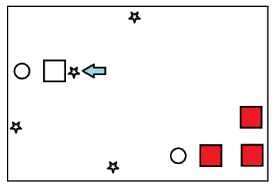
\includegraphics[width=\textwidth]{images/STARS.png}\\[0pt]
\caption{Imagen de Stars corpus}
\label{fig-STARS}
%\vspace*{1cm}
\end{minipage}
\hspace*{0cm}
\begin{minipage}[b]{0.5\linewidth}
\centering
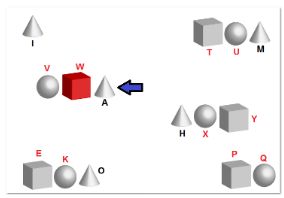
\includegraphics[width=\textwidth]{images/STARS2.png}\\[0pt]
\caption{Imagen de Stars2 corpus}
\label{fig-STARS2}
\end{minipage}
\end{figure}

%ejemplo minipage
%\begin{figure}
%\begin{minipage}[b]{0.5\linewidth}
%\centering
%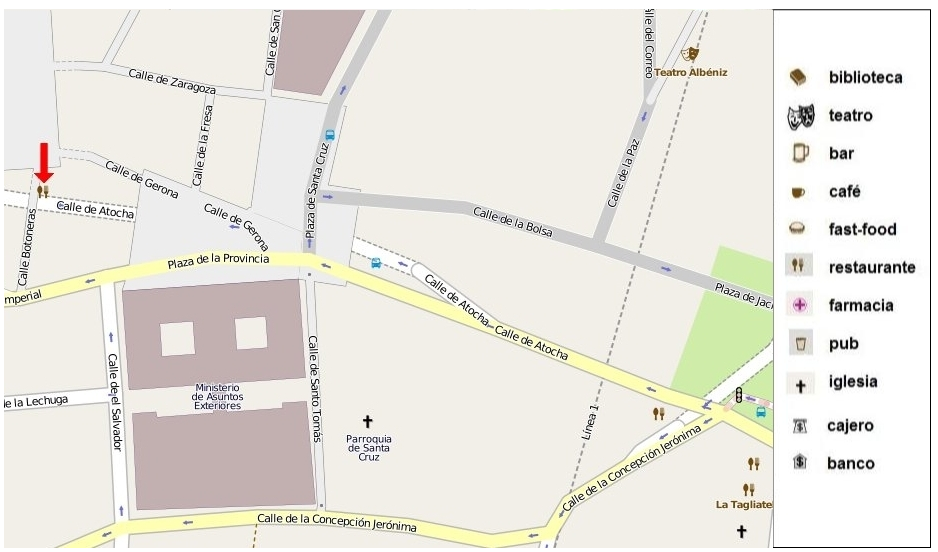
\includegraphics[width=\textwidth]{figures/rest-singular2x.png}\\[0pt]
%\caption{Target singular con zoom 2X}
%\label{rest-singular2x}
%\end{minipage}
%\vspace*{.1cm}
%\begin{minipage}[b]{0.5\linewidth}
%\centering
%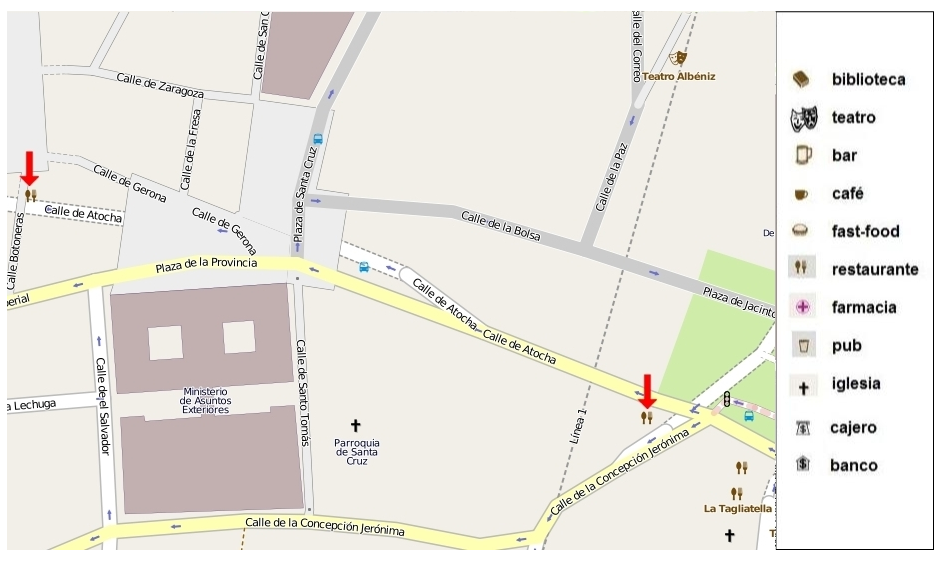
\includegraphics[width=\textwidth]{figures/rest-plural2x.png}\\[0pt]
%\caption{Target plural con zoom 2X}
%\label{rest-plural2x}
%\end{minipage}
%\end{figure}




%Despite their usefulness and general contribution to the research in REG, the above domains are still at a certain distance from the kinds of visual scene that might be required for a practical, real-world application. The need for additional complexity and/or realism, and our own interest in the surface realisation task for the Spanish and Portuguese languages, has led us to build a new computational resource of this kind. This work is described in the next sections. Further discussion on the differences between the Zoom corpus and existing resources is presented in Sec. \ref{sec-annotation}. 



\subsection{Trabajos emp\'iricos en el \'area}

%http://link.springer.com/chapter/10.1007/978-3-642-15573-4_9
%http://www.jetteviethen.net/papers/DaleViethen2010chapter.pdf

La investigaci\'on presentada en \cite{viethen-phd} se basa en dos premisas fundamentales: que la investigaci\'on
en la generaci\'on autom\'atica de expresiones referenciales debe esforzarse por lograr
sistemas que den salidas tan similar a la humana como sea posible; y que, para ello, debemos
esforzarnos para modelar el comportamiento humano como se puede observar en corpora.

La adopci\'on de estas premisas sirve para dos fines: en primer lugar, mejora la adecuaci\'on
de la salida de algoritmos de GER para el objeto target imitando la capacidad humana
de producir referencias adecuadas; y en segundo lugar, el estudio de corpus de datos producidos por humanos
 y algoritmos en desarrollo que pueden replicar estos datos podr\'ian
acercarnos a la comprensi\'on de que es lo que hacen los humanos cuando dan una ER.\\

Se\~nala que el cl\'asico algoritmo de GER y la mayor parte de sus descendientes no se basaron ni evaluaron contra datos producidos por humanos. Ellos se basaron en una visi\'on bastante minimalista de lo que se necesita
para que una expresi\'on referencial sea \'optima, concentr\'andose en la eficiencia computacional 
 y descripciones breves como sus principales preocupaciones.\\

 Existe un peque\~no n\'umero de enfoques que 
 se basaron en observaciones del comportamiento de referencia general humana
que obtuvieron a partir de experimentos psicoling\"u\'isticos, pero de nuevo no fueron evaluados
contra datos humanos.\\

Los algoritmos que se presentaron a los desaf\'ios de evaluaci\'on \cite{gatt-balz-kow:2008:ENLG} y \cite{reg2009}
fueron probados en el TUNA-Corpus, y algunos de ellos
tambi\'en tuvieron en cuenta los patrones que se encontraban en el conjunto del desarrollo. Pero hay una serie de preocupaciones en torno a la pregunta de si el TUNA-Corpus, y la forma de salida de los sistemas que se compar\'o 
en los desaf\'ios eran ideales para una evaluaci\'on de la adecuaci\'on descriptiva de GER.\\
%saque esto porque no se entiende
%A partir de los desaf\'ios que se describen en m\'as detalle y para evaluarlos en una serie de datos m\'as grande
%que contiene m\'as de una expresi\'on referencial para cada elemento est\'imulo.
Aborda tres \'areas principales en las que los corpus se puede utilizar para
promover el objetivo de la semejanza humana en la investigaci\'on sobre generaci\'on de expresiones referenciales:
evaluaci\'on, la recolecci\'on de corpus y an\'alisis y modelizaci\'on estad\'istica de
datos de corpus.\\
Comenz\'o con el an\'alisis del estado del arte de la investigaci\'on en
la generaci\'on de descripciones distintivas, trabaj\'o con relaciones espaciales y en el trabajo us\'o datos de corpus. Examin\'o una serie de opciones metodol\'ogicas que tienen que hacerse cuando se trabaja con los corpus de GER. Aqu\'i, explor\'o diferentes opciones para los desaf\'ios de recopilaci\'on de corpus, que se centran en torno al equilibrio que se necesita
entre el control de los par\'ametros experimentales tanto como sea necesario
y mantener la configuraci\'on de lo m\'as natural posible. Discuti\'o una serie de conceptos
que son de importancia para el an\'alisis de corpora de GER, tales como la naturalidad de diferentes
propiedades de los objetos, y las nociones de minimalidad y cuestiones de sobre-especificaci\'on de expresiones referenciales. Por \'ultimo, analiz\'o diferentes maneras en que la salida de un sistema se puede
comparar con los datos de corpora, bajo la premisa de que el objetivo de la comparaci\'on es
para evaluar si el sistema podr\'ia tener un modelo adecuado del comportamiento humano para la generaci\'on de expresiones referenciales.
Realiz\'o una investigaci\'on en las tres \'areas donde se puede emplear corpora en GER: Evaluaci\'on de semejanza humana, recopilaci\'on y an\'alisis de corpus, y modelado de datos de corpus. Realiz\'o un experimento de evaluaci\'on con tres de los algoritmos cl\'asicos, (1989) Algoritmo Greedy de Dale (Greedy), Dale y Haddock (1991b), Algoritmo Relacional (ra) Y Dale y Reiter (1995) Algoritmo Incremental (IA), Se pusieron a prueba en cuanto a su capacidad de
replicar las expresiones referenciales se encuentran en un grupo relativamente peque\~no de corpus de expresiones referenciales
en un dominio visual de im\'agenes puestas en una grilla.
%de rejilla de cajones de armarios ling. 
En el an\'alisis de este experimento tuvo dos resultados principales: (1) que identic\'o en particular tres 
fen\'omenos que todav\'ia plantean importantes retos para los algoritmos GER con el objetivo de replicar
el comportamiento humano, y (2) que proporciona una plataforma para la discusi\'on de una serie de
dificultades que se presentan para la evaluaci\'on basada en corpus de GER. Esto result\'o en una serie
de criterios para el dise\~no de los dos corpus que el trabajo en el resto de la tesis.
Los tres fen\'omenos en las expresiones referenciales producidas por humanos que los
algoritmos probados no fueron capaces de replicar satisfactoriamente sobre-especificaci\'on,
relaciones espaciales, y comportamiento de voluntarios espec\'ificos. Ambos
Greddy y la IA fueron capaces de generar algo de la redundancia que se encontr\'o en el corpus.
 Ni Greedy ni el IA estaban dise\~nados para ser capaz de generar expresiones referenciales que contengan relaciones entre entidades, pero el ra fue dise\~nado para incluirlas. Sorprendentemente, el
ra no s\'olo fallo en generar cualquiera de las descripciones contenidas en el corpus de evaluaci\'on; sino tambi\'en que las descripciones que se gener\'o parec\'ian m\'as como enigmas cuyo objetivo era confundir a un oyente, m\'as que ayudar en
los intentos de se\~nalar el objetivo referente. 

Una valoraci\'on te\'orica de otras aproximaciones dise\~nados para manejar las relaciones estableci\'o que ninguno de ellos incluir\'ia una relaci\'on, si no es absolutamente necesaria para distinguir el target.
La tercera observaci\'on que el experimento dejo a la vista fue que la gente no siempre hace lo mismo en la misma situaci\'on. De hecho, incluso la misma persona podr\'ia describir el mismo target de diferente manera en distintas
circunstancias. 

 None of the algorithms tested were intended to take such inter- and
intra-speaker variation into account, and only very recently have implementations
of the
ia
begun to model speaker-preferences to some degree.

No se pretend\'ia que ninguno de los algoritmos de la prueba tomara en cuenta las variaciones entre-hablantes, ni del mismo hablante. Hay implementaciones del IA que han comenzado a agregar modelo de preferencias de hablante en alg\'un grado.

Los temas generales con evaluaci\'on basada en corpus que esta experiencia de evaluaci\'on dej\'o
al descubierto fueron (1) la interdependencia estrecha entre algoritmos y la
representaci\'on subyacente de conocimiento que utilizan, (2) el no-determinismo de la generaci\'on del lenguaje natural, (3) la cuesti\'on de c\'omo comparar la salida algoritmos con gold-standar, y (4) el dominio espec\'ifico de los algoritmos de GER.\\
La discusi\'on de estos temas ha dado lugar a la siguiente lista de Evaluaci\'on en GER basado en corpus:

1. Si el corpora est\'a destinado para ser reutilizado para la evaluaci\'on comparativa de diferentes
algoritmos, una representaci\'on subyacente del dominio debe ser proporcionada para ser usada por todos los algoritmos.

2. Si queremos confiar en los resultados, el corpus debe contener tantos casos como sea posible de tantos direntes hablantes como sea posible para cada escenario referencial. 
Esto es cierto si un algoritmo es evaluado en t\'erminos de ser capaz de generar una expresi\'on referencial que suene natural, o si est\'a probado por su probabilidad de pertenecer a un modelo espec\'ifico de conducta humana de referencia, mediante la comprobaci\'on de si se puede generar todas las descripciones en un corpus.

3. Si la probabilidad de un algoritmo de ser un modelo de la conducta humana de referencia
se eval\'ua, deben utilizarse m\'etricas basadas en recuento (RECALL) y precisi\'on (PRESITION). En este
caso, el conjunto completo de las descripciones que el algoritmo proporciona para cada
escenario de referencia en virtud de cualquier ajuste de par\'ametro debe ser comparado con el
conjunto de las descripciones contenidas en el corpus para el mismo escenario referencial.
Si la capacidad m\'as orientada a la aplicaci\'on para generar una referencia es similar a la humana
se ha de evaluar, s\'olo una descripci\'on por escenario.
Esto debe hacerse utilizando m\'etricas basadas en la precisi\'on para probar c\'omo muchos de las
descripciones dadas por los algoritmos est\'an contenidas en el corpus.
4. Algoritmos que son juzgados en un dominio espec\'ifico c, no se debe asumir como
f\'acilmente adaptable a otros dominios. Idealmente, los corpus que abarcan muchos diferentes
deben estar disponibles para las pruebas de los algoritmos que generalizan en distintos tipos de dominios.
Realiz\'o 2 corpus el GRE3D3 y el GRE3D7 descriptos en \ref{sec:corpus2}

Trabaj\'o con \'arboles de decisi\'on ...
\textcolor{blue}{Aca agregar otras personas que usaron corpus para generacion de ER, Ivandre... }

%http://www.lrec-conf.org/proceedings/lrec2012/pdf/152_Paper.pdf
En el trabajo \ref{ivandre-work-corpus} presentan 2 alternativas para aprender la seleccio\'on de atributos de una expresi\'on referencial a partir de corpus. Toma los caracter\'isticas de aprendizaje como el conjunto de valores enteros que representan el poder discriminativo de cada atributo (es decir, el n\'umero de distractores que cada atributo elimina por cada atributo que tiene el target, ejemplos son color, tama\~no, etc.) 
 %For instance, in a context set as
%seen in previous Example 1, assuming that we would like to
%refer to E4, the corresponding discriminatory power values
%would be defined as d type =1, d size =1 and d colour =3.
%In the first learning method, we will attempt to learn possible
%Pj orderings (defined as nominal values) that, if applied
%to  the  Incremental  algorithm,  would  produce  the  desired
%output L for each given input C. In the second method, we
%will  use  the  input  C  to  (binary)  decide  whether  to  select
%each attribute individually.  We will call these our
%Global and Individual AS  classifiers,  which  are  discussed  sepa-
%rately below

\subsection{M\'etricas de evaluaci\'on/comparaci\'on con corpus}

Para medir la performance de los algoritmos podemos usar m\'etricas autom\'aticas o m\'etricas manuales, las m\'etricas autom\'aticas son aquellas que se calculan mediante un algoritmo y las manuales en las cuales les requerimos a personas que evaluen las expresiones referenciales.


\subsubsection{M\'etricas autom\'aticas}


La exactitud (Accuracy) se define como el porcentaje de coincidencias exactas entre cada RE producida por un ser humano y la producida por el sistema para la misma escena y target. Se considera que es una m\'etrica demasiado estricta.\\


El coheficiente Dice es una m\'etrica de comparaci\'on de conjuntos, el valor va entre 0 y 1, 1 indica un perfecto match entre los conjuntos. Para dos conjuntos A y B, Dice se calcula como sigue:\\

$Dice(A,B) = \frac{2\times|A \cap B|}{|A|+|B|}$\\

\textsc{masi} de \cite{Passonneau06measuringagreement}~es una adaptaci\'on de el coheficiente Jaccard el cual varia en favor de la similaridad cuando un conjunto es un subconjunto de otro, como Dice varia entre 0 y 1, 1 indica match perfecto. Se calcula como sigue:\\
%which biases it in favor of similarity where one set
%is a subset of the other. Like Dice, it ranges between
%0 and 1, where 1 indicates a perfect match. It is computed as follows:\\

$\textsc{masi}(A,B) = \delta \times \frac{|A \cap B|}{|A \cup B|}$ \\


donde $\delta$ es un coheficiente definido como sigue:\\


 \begin{equation}
     \delta  = \left\{
	       \begin{array}{ll}
		 0      & if A \cap B = \emptyset \\
		 1 & if A = B  \\
		 \frac{2}{3}     & if A \subset B ~or~ B \subset A\\
		 \frac{1}{3}     & otherwise
	       \end{array}
	     \right.
 \end{equation}

Intuitivamente significa que se prefieren aquellas descripciones producidas por el sistema las cuales no incluyen atributos que los humanos no incluyeron.
%Intuitively, this
%means that those system-produced descriptions are
%preferred which do not include attributes that are
%omitted by a human.  

\subsubsection{M\'etricas manuales}
\textcolor{blue}{aca me falta escribir, aunque no se si no poner todo esto en parte evaluacion}

\chapter{Introducci\'on a la L-simulaci\'on}
\label{sec:intro_logica}

mover a intro... y linkear con est capitulo...

No existe un acuerdo general sobre la representaci\'on b\'asica de
tanto la entrada y la salida del problema de GER; esto se maneja m\'as bien de manera ad-hoc
por cada nueva propuesta.

\cite{Krahmer2003} usan grafos dirigidos etiquetados en el contexto de este problema: los grafos son lo suficientemente abstractos 
para expresar un gran n\'umero de dominios y hay muchos algoritmos conocidos para tratar
con este tipo de estructuras. 

De hecho, no se trata de otra cosa que una representaci\'on alternativa de los modelos relacionales, usada t\'ipicamente 
para proporcionar sem\'antica a los lenguajes formales como el de primer orden y l\'ogicas de orden superior, l\'ogicas modales, etc.


Exactamente debido a su generalidad, los grafos no definen por s\'i mismos, una \'unica noci\'on de igualdad. Cu\'ando decimos 
que dos nodos en el grafo pueden o no pueden ser
referenciados de forma \'unica en t\'erminos de sus propiedades? Esta pregunta s\'olo tiene sentido una vez que ya hemos 
fijado un cierto nivel de expresividad el cual determina cuando dos grafos, o dos elementos en el mismo gr\'afo, son equivalentes.

La expresividad se puede formalizar usando las relaciones estructurales de los grafos (isomorfismos, etc.) o, alternativamente, 
lenguajes l\'ogicos. 

%Ambas formas se presentan en Secci\'on \ref{sec:estructurales}, donde tambi\'en 
Discutiremos la noci\'on de impacto de expresividad 
en los casos que el problema GRE tiene soluci\'on; la complejidad computacional de los algoritmos GER involucrados; 
y la complejidad computacional del problema de la realizaci\'on. Luego investigamos el problema GER en t\'erminos de diferentes 
nociones de expresividad. 


\section{Seleccionando el lenguaje}


Las estructuras relacionales son muy adecuadas para la representaci\'on de situaciones o escenas. La estructura relacional (tambi\'en llamado ``el modelo relacional'') es un conjunto no vac\'io de objetos -el dominio- junto con una colecci\'on de las relaciones, cada uno con una aridad fija.
Formalmente, asumimos un vocabulario fijo y finito (pero arbitrario) de
s\'imbolos de relaci\'on n-aria (las constantes y s\'imbolos de funci\'ones pueden ser representados como relaciones de aridad adecuada). 


Un modelo relacional $\+M$ es una tupla 
$\tup{\Delta,\interp{\cdot}}$ donde $\Delta$ es un conjunto no vac\'io, y
$\interp{\cdot}$ es una funci\'on de interpretaci\'on, esto es,
$\interp{r} \subseteq \Delta^n$ para todo s\'imbolo de relaci\'on $n$-aria tal que
$r$ est\'a en el vocabulario. $\+M$ es \emph{finito} cuando
$\Delta$ es finito.  El \emph{tama\~no} de un modelo $\+M$ es la suma
$\#\Delta + \#\interp{\cdot}$, donde $\#\Delta$ es la cardinalidad
de $\Delta$ y $\#\interp{\cdot}$ es la suma de todas las aridades de las
relaciones en $\interp{\cdot}$.

Vamos a presentar 2 ejemplos, uno en el que los tenemos agentes (perros y gatos),y otro en el que el dominio son cosas es decir, es de alguna manera est\'atico.

El primer ejemplo se muestra en la Figura~\ref{fig:cat-dog-1} en la cual hemos representado una escena
como un modelo relacional. Intuitivamente, $a$, $b$ y $d$ son dogs, mientras que 
$c$ y $e$ are cats;  $d$ es un small beagle;
 $b$ y $c$ son tambi\'en small.
 Leeremos $\aSniffing(d,e)$ como ``{\em $d$ is sniffing $e$}''.

 \begin{figure}
 \begin{center}
 \begin{tabular}{rcl}
$\Delta$               & = & $\cset{a,b,c,d,e}$\\
$\interp{\nDog}$      & = & $\cset{a,b,d}$\\
$\interp{\nCat}$      & = & $\cset{c,e}$\\
$\interp{\nBreed}$    & = & $\cset{d}$\\
$\interp{\aSmall}$    & = & $\cset{b,c,d}$\\
$\interp{\aSniffing}$ & = & $\cset{(a,a),(b,a),(c,b),(d,e),(e,d)}$
 \end{tabular}
\begin{picture}(120,50)
\put(0,-50){\begin{tikzpicture}
  [
    n/.style={circle,fill,draw,inner sep=1.5pt,node distance=1.5cm},
    aSniffing/.style={->, >=stealth, semithick, shorten <= 3pt, shorten >= 3pt},
  ]
 \node[n,label=above:$a$,label=below:{\relsize{-1}$\begin{array}{c}\nDog\end{array}$}] (a) {};

 \node[n,label=above:$b$,label=below:{\relsize{-1}$\begin{array}{c}\nDog\\ \aSmall \end{array}$}, right of=a] (b) {};

 \node[n,label=above:$c$,label=below:{\relsize{-1}$\begin{array}{c}\nCat\\ \aSmall\end{array}$}, right of=b] (c) {};

 \node[n,label=above left:$d$,label=below:{\relsize{-1}$\begin{array}{c}\nDog\\ \nBreed\\  \aSmall \end{array}$}, below of=a,xshift=25pt,yshift=-10pt] (d) {};

 \node[n,label=above right:$e$,,label=below:{\relsize{-1}$\begin{array}{c}\nCat\end{array}$},right of=d] (e) {};

 \draw [aSniffing,loop left] (a) to node[above,xshift=-5pt]{\relsize{-1}$\aSniffing$} (a);

 \draw [aSniffing,bend right=40] (b) to node[auto,swap]{\relsize{-1}$\aSniffing$} (a);

 \draw [aSniffing,bend right=40] (c) to node[auto,swap]{\relsize{-1}$\aSniffing$} (b);

 \draw[aSniffing, bend left=40] (d) to node[auto]{\relsize{-1}$\aSniffing$} (e);
 \draw[aSniffing, bend left=40] (e) to node[auto,swap]{\relsize{-1}$\aSniffing$} (d);

 \end{tikzpicture}}
 \end{picture}

 \end{center}
 \caption{Representaci\'on de escenas de Graph $\+S$.\label{fig:cat-dog-1}}
 \end{figure}





El segundo ejemplo se muestra en la Figura~\ref{grafo-GRE3D7-stimulus_b} en el que hemos representado el Contexto \ref{GRE3D7-stimulus1} 
como un modelo relacional. $e_1$,$e_3$,$e_5$, son 'ball', $e_2$, $e_6$ y $e_7$, son 'cube', mientras que 
$e_1$, $e_3$ y $e_6$ son 'yellow', $e_2$, $e_4$, $e_5$, $e_7$ son 'red';
%Para las relaciones tenemos $\Ontop(e_3,e_2)$ como ``{\em $e_3$ on top of $e_2$}''.
%$\Rightof(e_4,e_5)$, $\Rightof(e_6,e_7)$, $\Lefttof(e_5,e_4)$,$\Leftof(e_7,e_6)$. $e_4$ y $e_5$ son 'large', los dem\'as 'small'.

\begin{figure}
\begin{flushleft}
\begin{tabular}{rcl}
$\Delta$              & = & $\cset{e_1,e_2,e_3,e_4,e_5,e_6,e_7}$\\
$\interp{\aRed}$      & = & $\cset{e_2,e_4,e_5,e_7}$\\
$\interp{\aYellow}$   & = & $\cset{e_1,e_3,e_6}$\\
$\interp{\nBall}$     & = & $\cset{e_1,e_3,e_6}$\\
$\interp{\nCube}$     & = & $\cset{e_2,e_4,e_7}$\\

$\interp{\aSmall}$    & = & $\cset{e_1,e_2,e_3,e_6,e_7}$\\
$\interp{\aLarge}$    & = & $\cset{e_4,e_5}$\\

$\interp{\nRightof}$   & = & $\cset{(e_4,e_5),(e_6,e_7)}$\\
$\interp{\nLeftof}$    & = & $\cset{(e_5,e_4),(e_7,e_6)}$\\
$\interp{\nOntop}$     & = & $\cset{(e_3,e_2)}$\\

 \end{tabular}
\begin{picture}(120,50)
\put(0,-50){\begin{tikzpicture}
  [
    n/.style={circle,fill,draw,inner sep=1.5pt,node distance=1.5cm},
		 aArrow/.style={->, >=stealth, semithick, shorten <= 1pt, shorten >= 1pt},
    %aSniffing/.style={->, >=stealth, semithick, shorten <= 3pt, shorten >= 3pt},
  ]
%\begin{tikzpicture}
%  [
%    n/.style={circle,fill,draw,inner sep=3pt,node distance=2cm},
%    aArrow/.style={->, >=stealth, semithick, shorten <= 1pt, shorten >= 1pt},
%  ]
 \node[n,label=above:$e_1$,label=below:{
    \relsize{-2}$\begin{array}{c}
      \nSmall\\[-3pt] 
      \nYellow \\[-3pt] 
      \nBall\end{array}$}] (a) {};
 \node[n,label=above:$e_2$,label=below:{
    \relsize{-2}$\begin{array}{c}     
      \nSmall\\[-3pt] 
      \nRed\\[-3pt] 
      \nCube\end{array}$}, right of=a] (b) {};
 \node[n,label=below:$e_3$,label=above:{
    \relsize{-2}$\begin{array}{c}
      \nTop\\[-3pt]      
      \nSmall\\[-3pt] 
      \nYellow\\[-3pt] 
      \nBall\end{array}$}, above of=b] (c) {};
 \node[n,label=right:$e_4$,label=left:{
    \relsize{-2}$\begin{array}{c}
      \nLarge\\[-3pt] 
      \nRed\\[-3pt] 
      \nCube\end{array}$}, right of=b] (d) {};
 \node[n,label=left:$e_5$,label=below:{
    \relsize{-2}$\begin{array}{c}
      \nLarge\\[-3pt] 
      \nRed\\[-3pt] 
      \nBall\end{array}$}, right of=d] (e) {};
 \node[n,label=right:$e_6$,label=left:{
    \relsize{-2}$\begin{array}{c}
      \nSmall\\[-3pt] 
      \nYellow\\[-3pt] 
      \nCube\end{array}$}, right of=e] (f) {};
 \node[n,label=left:$e_7$,label=below:{
    \relsize{-2}$\begin{array}{c}
      \nSmall\\[-3pt]
      \nRed\\[-3pt] 
      \nCube\end{array}$},  right of=f] (g) {};
 \draw [aArrow,bend right=40] (b) to node[auto,swap]{\relsize{-3}$\nBelow$} (c);
 \draw [aArrow,bend right=40] (c) to node[auto,swap]{\relsize{-3}$\nOntop$} (b);
 \draw [aArrow,bend right=40] (d) to node[auto,swap]{\relsize{-3}$\nLeftof$} (e);
 \draw [aArrow,bend right=40] (e) to node[auto,swap]{\relsize{-3}$\nRightof$} (d);
 \draw [aArrow,bend right=40] (f) to node[auto,swap]{\relsize{-3}$\nLeftof$} (g);
 \draw [aArrow,bend right=40] (g) to node[auto,swap]{\relsize{-3}$\nRightof$} (f);
 \draw[dotted] (-0.5,-1.1) rectangle (8,2.6);

% \end{tikzpicture}
%\caption{Grafo del contexto \ref{GRE3D7-stimulus}}
%\label{grafo-GRE3D7-stimulus_b}
%\end{figure}
 \end{tikzpicture}}
 \end{picture}
 \end{flushleft}
 \caption{Representaci\'on del Contexto \ref{GRE3D7-stimulus1}}
 \label{grafo-GRE3D7-stimulus_b}
 \end{figure}


Los languajes l\'ogicos son \'utiles para la tarea de describir (formalmente) elementos de una estructura relacional. 

Por ejemplo, el lenguaje cl\'asico
de la l\'ogica de primer-orden (con desigualdad), \FOL, dado por:
$$
  \top \mid x_i \not\approx x_j \mid  r (\bar x) \mid \lnot \gamma \mid \gamma \land \gamma' \mid \exists x_i . \gamma
$$
%
donde $\gamma,\gamma' \in \FOL$,
$r$ es un s\'imbolo de relaci\'on $n$-aria y $\bar x$ es una tupla de $n$ variables.
Como es usual, $\gamma \lor \gamma'$ y $\forall x . \gamma$ son las versiones cortas de
$\lnot(\lnot\gamma \land \lnot\gamma')$ y $\lnot\exists x . \lnot\gamma$, respectivamente.
F\'ormulas de la forma $\top$, $x_i \not\approx x_j$ y $r(\bar
x)$ son llamados \emph{atomos}.%
  \footnote{%
    Por razones t\'ecnicas, incluimos el s\'imbolo de desigualdad symbol $\not \approx$ como
    primitivo. La igualdad puede ser definida usando negaci\'on.
  }
Dado un modelo relacional $\+M = \tup{\Delta,\interp{\cdot}}$ y una
f\'ormula $\gamma$ con variables libres%
\footnote{%
    W.l.o.g.\ asumimos que cada variable no puede aparecer libre y ligada a la vez, que una variable no esta ligada 2 veces,
    y que el \'indice de las variables crece en la f\'ormula de izquierda a derecha.%
}
entre $x_1\ldots x_n$, inductivamente definimos la \emph{extensi\'on} o
\emph{interpretaci\'on} de $\gamma$ como el conjunto de $n$-tuplas
 $\interp{\gamma}^n \subseteq \Delta^n$ que satisface:

\begin{center}
\begin{tabular}{rcl@{\hspace{1cm}}rcl}
$\interp{\top}^n$ &$=$& $\Delta^n$
&
$\interp{x_i \not\approx x_j}^n$ &$=$& $\cset{\bar{a} \mid \bar{a} \,{\in}\, \Delta^n, a_i \neq a_j}$
\\
$\interp{\lnot\delta}^n$ &$=$& $\Delta^n \setminus \interp{\delta}^n$
&
$\interp{r (x_{i_1} \ldots x_{i_k})}^n$ & $=$&$\cset{\bar{a} \mid \bar{a} \,{\in}\, \Delta^n, (a_{i_1} \ldots a_{i_k}) {\in} \interp{r}}$
\\
$\interp{\delta \land \theta}^n$ &$=$& $\interp{\delta}^n \cap \interp{\theta}^n$
&
$\interp{\exists x_{l}.\delta}^n$ &$=$& $\cset{\bar a \mid \bar a  e  \in \interp{\delta'}^{n+1}\ \text{for some $e$}}$
\end{tabular}
\end{center}
%
donde $1 \le i,j, i_1, \ldots, i_k \le n$, $\bar{a} = (a_1\ldots
a_n)$, $\bar{a}e = (a_1\ldots a_n,e)$ y $\delta'$ son
obtenidos reeplazando todas las ocurrencias de $x_l$ en $\delta$ por
$x_{n+1}$. 
%Cuando la cardinalidad de las tuplas involucradas en el contexto es conocida 
%escribiremos $\interp{\gamma}$ en lugar de
%$\interp{\gamma}^n$.

Con una sintaxis y sem\'antica de un lenguaje en mente, podemos formalmente definir el problema de L-GRE para un conjunto target de elementos T %(ligeramente adaptaremos la definici\'on en ~\cite{arec2:2008:Areces}):

\medskip
\noindent
{\small
\begin{center}
\begin{tabular}{ll} \hline
\multicolumn{2}{l}{
\textsc{Problema $\gL$-GRE }}\\ \hline
\ \ Input: & un model $\gM=\tup{\Delta,\interp{\cdot}}$ y un conjunto target no vac\'io $T \subseteq \Delta$.\\
\ \ Output: & una f\'ormula $\varphi \in \gL$ tal que
$\interp{\varphi} = T$ si existe, y $\bot$ caso contrario.\\ \hline
\end{tabular}
\end{center}}
Cuando el output es no $\bot$, decimos que $\phi$ es una
\emph{expresi\'on referencial en $\+L$ (ER-$\+L$) para $T$ en $\+M$}.

La salida de el problema $\+L$-GRE es una f\'ormula de
$\+L$ cuya interpretaci\'on en el modelo de input $\gM$ es el conjunto target, si
esa f\'ormula existe. 


% Esta definici\'on aplica incluso a la GRE para
%objetos  de el dominio teniendo un conjunto singleton como target.

Consideramos solo modelos relacionales con s\'imbolos de relaciones unarios y binarios, usaremos $p$ para las proposiciones (propiedades) y $r$ para los s\'imbolos de relaci\'on binarias.


Seleccionando el lenguaje apropiado...

Dado un modelo M, podr\'ia haber un infinito n\'umero de f\'ormulas que de forma \'unica
describan al target (incluso f\'ormulas que no son l\'ogicamente equivalentes podr\'ian tener
la misma interpretaci\'on una vez al modelo este fijo). 


Por ejemplo en el Contexto \ref{GRE3D7-stimulus1} $\aLarge \nBall$ y $\aRed \nBall$ son diferentes f\'ormulas pero tienen la misma interpretaci\'on en $+M$.

Como es bien conocido en la comunidad de generaci\'on autom\'atica de lenguaje natural, diferentes
realizaciones del mismo contenido podr\'ian dar lugar a expresiones referenciales que son m\'as o menos
apropiadas en el contexto dado. 

Argumentamos que la generaci\'on de contenido usando lenguajes con diferente poder expresivo puede tener un impacto en la estapa posterior
de realizaci\'on sint\'actica (surface realization).

F\'ormulas que identifican a $b$ en nuestro primer ejemplo

\begin{table}
$$
\begin{array}{cl}
 \gamma_1: & \nDog(x) \land \aSmall(x) \land
   \exists y . (\aSniffing(x,y) \land \nDog(y))\\[3pt]
  %
  \gamma_2: & \nDog(x) \land \aSmall(x) \land
  \forall y . (\neg \nCat(y) \lor \neg \aSniffing(x,y))\\[3pt]
  %
  \gamma_3: & \nDog(x) \land
  \exists y . (x \not\approx y \land \nDog(y)  \land \aSniffing(x,y))\\[3pt]
  %
  \gamma_4: & \nDog(x) \land
  \exists y . (\nCat(y) \land \aSmall(y) \land \aSniffing(y,x))
  %
 \end{array}
$$
\caption{Descripciones alternativas para el objeto $b$ en el modelo mostrado en Figura~\ref{fig:cat-dog-1}.}\label{tab:gammas}
\end{table}

Restringiendo la determinaci\'on de contenido a FO-, aseguramos que f\'ormulas como  $\gamma_2$ no se generar\'an. Si prohibimos el distinto del lenguaje  $\gamma_3$ tambi\'en queda exclu\'ida.

El hecho de que el lenguaje de representaci\'on utilizado tiene un impacto sobre la determinaci\'on de contenido es obvio, pero no ha recibido la atenci\'on que merece. Areces et al. [1] usaron diferentes l\'ogicas de descripci\'on (una familia de lenguajes formales utilizado en representaci\'on del conocimiento, vea [2]) para clasificar y dar un marco formal para
trabajo previo sobre GRE. Vamos a presentar r\'apidamente algunas de estos lenguajes ya que los mencionaremos en las siguientes secciones. Usando l\'ogicas de descripci\'on en lugar de fragmentos de FO es s\'olo una cuesti\'on de notaci\'on, como la mayor\'ia de l\'ogicas descriptivas se pueden ver
fragmentos como impl\'icitas de FO. Por ejemplo, el lenguaje de la l\'ogica de descripci\'on ALC, se define sint\'acticamente como el conjunto de f\'ormulas,
$$
\top \mid p \mid \neg \gamma \mid \gamma \wedge \gamma' \mid  \exists r. \gamma
$$
(donde $p$ es un s\'imbolo proposicional, $r$ s\'imbolo relacional binario, y $\gamma,\gamma' \in \ALC$) corresponde al fragmento sint\'actico de
\FOL sin $\not\approx$, como es mostrado por la traducci\'on est\'andar $\st_x$:

\begin{center}
\begin{tabular}{rcl@{\hspace{1cm}}rcl}
$ \st_{x_i}(\top)$ &$=$& $\top$
&
$\st_{x_i}(\gamma_1 \land \gamma_2)$ &$=$& $\st_{x_i}(\gamma_1) \land \st_{x_i}(\gamma_2)$
\\
  $\st_{x_i}(p)$ &$=$& $p(x_i)$
&
$\st_{x_i}(\exists r . \gamma)$ &$=$& $\exists x_{i+1} . (r(x_i,x_{i+1}) \land \st_{x_{i+1}}(\gamma))$
\\
 $\st_{x_i}(\lnot \gamma)$ &$=$& $\lnot\st_{x_i}(\gamma)$
&
\end{tabular}
\end{center}

En efecto, dado un modelo relacional $\+M$, la extensi\'on de una f\'ormula \ALC en M coincide exactamente con la extensi\'on de $\st_{x_1}(\varphi)$ (v\'ease, por ejemplo, ~\cite{baad:desc03}). Gracias
a este resultado, para cualquier f\'ormula $\varphi$ de \ALC y sus sublenguajes podemos definir $\interp{\varphi} = \interp{\st_{x_1}(\varphi)}$.
 Volviendo a nuestro ejemplo anterior, mediante la restricci\'on de contenido
generaci\'on en f\'ormulas $\ALC$ (o equivalentemente, el fragmento correspondiente de \FOL)
evitar\'iamos f\'ormulas como
$\gamma_3$ (sin igualdad) y
$\gamma_4$ (aparece cuanti elemento ed
siempre en segunda posici\'on de argumento).
Generaci\'on se discute en ~\cite{AKS08}, en t\'erminos de diferentes l\'ogicas de descripci\'on como \ALC
y \EL (\ALC sin negaci\'on). Vamos a ampliar los resultados en ese papel, con-
Sidering por ejemplo \ELAN (\ALC con la negaci\'on permitida s\'olo frente a relaciones unarias), pero, en general, nosotros tomamos un enfoque modelo te\'orico y argumentamos que la cuesti\'on principal no es si se debe utilizar una u otra (descripci\'on l\'ogica para la generaci\'on de contenido, sino que son el diferencias sem\'antica a tener en cuenta. Esto no solo determina el formalismo l\'ogico requerido sino tambi\'en impacta tanto en la determinaci\'on de contenido como en los problemas de realizaci\'on sint\'actica. Cada
lenguaje l\'ogico puede ser visto como un compromiso entre la expresividad, realizabilidad y complejidad computacional. La selecci\'on apropiada para una tarea GRE particular, debe depender del contexto actual




Para el segundo ejemplo: \\
Supongamos que queremos identificar a $e_5$ del Contexto \ref{GRE3D7-stimulus-conLetras}, las siguientes son f\'ormulas que identifican a un\'ivocamente a $e_5$ en el contexto considerado.

\begin{table}
$$
\begin{array}{cl}
 \gamma_1: & \aRed(x) \land \nBall(x)\\[3pt]
  %
 \gamma_2: & \aLarge(x) \land \nBall(x)\\[3pt]
  %
 \gamma_3: & \nLarge(x) \land \aRed(x) \land \nBall(x)\\[3pt]
  %
 \gamma_4: & \nLarge(x) \land \aRed(x) \land \nBall(x) \land
   \exists y . (\nRightof(x,y) \land \aLarge(y) \land \aRed(y) \land \nCube(y))\\[3pt]
  %ex1
 \gamma_5: & \nLarge(x) \land \aRed(x) \land \nBall(x) \land
  \forall y . (\neg \nBall(y) \lor \neg \nRightof(x,y))\\[3pt]
  %ex 2
 \gamma_6: & \nLarge(x) \land \aRed(x) \land \nBall(x) \land
  \exists y . (x \not\approx y \land \nCube(y) \land \nRightof(x,y))\\[3pt]
  %ex 3
 \gamma_7: & \nLarge(x) \land \aRed(x) \land \nBall(x) \land
  \exists y . (\nCube(y) \land \aRed(y) \land \nLeftof(y,x))
  %ex 4
 \end{array}
$$
\caption{Descripciones alternativas para el objeto $e_5$ del Contexto~\ref{GRE3D7-stimulus-conLetras}.}\label{tab:gammas}
\end{table}

Notar que $\gamma_2$ y $\gamma_3$ son m\'inimas, es decir no se puede dar una f\'ormula m\'as corta que esas.
$\gamma_4$ se puede realizar como ``Large red ball right-of large red cube''. Esta f\'ormula junto con $\gamma_1$, $\gamma_2$ y $\gamma_3$ son caracterizadas como f\'ormulas positivas, conjuntivas y existenciales (no contienen negaci\'on y solo tienen conjunciones y cuantificadores existenciales), este tipo de f\'ormulas son las que m\'as se encuentran en corpus ~\cite{viethen06:_algor_for_gener_refer_expres,deemter06:_build_seman_trans_corpus_for,gre3d3}.

Bueno, pero entonces podemos elegir otra l\'ogca cuyo lenguaje este restringido a las ER que queremos generar.

Restringiendo la determinaci\'on de contenido a FO-, aseguramos que f\'ormulas como  $\gamma_5$ no se generar\'an. 
Si prohibimos el distinto del lenguaje  $\gamma_6$ tambi\'en queda exclu\'ida.

%El hecho de que el lenguaje de representaci\'on utilizado tiene un impacto sobre la determinaci\'on de contenido es obvio, 
%pero no ha recibido la atenci\'on que merece. 
%Areces et al. [1] usaron diferentes l\'ogicas de descripci\'on (una familia de lenguajes formales utilizado en 
%representaci\'on del conocimiento, vea [2]) para clasificar y dar un marco formal para
%trabajo previo sobre GRE. 

Usar l\'ogicas de descripci\'on en lugar de fragmentos de FO es s\'olo una cuesti\'on de notaci\'on, como la mayor\'ia de l\'ogicas 
descriptivas se pueden ver como
fragmentos de FO. Por ejemplo, el lenguaje de la l\'ogica de descripci\'on ALC, se define sint\'acticamente como el conjunto de f\'ormulas,
$$
\top \mid p \mid \neg \gamma \mid \gamma \wedge \gamma' \mid  \exists r. \gamma
$$
(donde $p$ es un s\'imbolo proposicional, $r$ s\'imbolo relacional binario, y $\gamma,\gamma' \in \ALC$) corresponde al fragmento 
sint\'actico de
\FOL sin $\not\approx$, como es mostrado por la traducci\'on est\'andar $\st_x$:

\begin{center}
\begin{tabular}{rcl@{\hspace{1cm}}rcl}
$ \st_{x_i}(\top)$ &$=$& $\top$
&
$\st_{x_i}(\gamma_1 \land \gamma_2)$ &$=$& $\st_{x_i}(\gamma_1) \land \st_{x_i}(\gamma_2)$
\\
  $\st_{x_i}(p)$ &$=$& $p(x_i)$
&
$\st_{x_i}(\exists r . \gamma)$ &$=$& $\exists x_{i+1} . (r(x_i,x_{i+1}) \land \st_{x_{i+1}}(\gamma))$
\\
 $\st_{x_i}(\lnot \gamma)$ &$=$& $\lnot\st_{x_i}(\gamma)$
&
\end{tabular}
\end{center}

En efecto, dado un modelo relacional $\+M$, la extensi\'on de una f\'ormula \ALC en $\+M$ coincide exactamente con la extensi\'on
 de $\st_{x_1}(\varphi)$ (v\'ease, por ejemplo, ~\cite{baad:desc03}). Gracias
a este resultado, para cualquier f\'ormula $\varphi$ de \ALC y sus sublenguajes podemos definir 
$\interp{\varphi} = \interp{\st_{x_1}(\varphi)}$.




 Volviendo a nuestro ejemplo anterior, mediante la restricci\'on de la generaci\'on de contenido
a f\'ormulas de $\ALC$ (o equivalentemente, el fragmento correspondiente de \FOL)
evitar\'iamos f\'ormulas como
$\gamma_5$ (sin igualdad) y

$\gamma_4$ (aparece cuanti elemento ed
siempre en segunda posici\'on de argumento). ESTE EJ NO LO PUSE... ver si consigo alguno interesante


%Generaci\'on se discute en ~\cite{AKS08}, en t\'erminos de diferentes l\'ogicas de descripci\'on como \ALC
%y \EL (\ALC sin negaci\'on). Vamos a ampliar los resultados en ese papel, consideando por ejemplo \ELAN 
%(\ALC con la negaci\'on permitida s\'olo frente a relaciones unarias), pero, en general, nosotros tomamos un enfoque modelo te\'orico y argumentamos que la cuesti\'on principal no es si se debe utilizar una u otra (descripci\'on l\'ogica para la generaci\'on de contenido, sino que son el diferencias sem\'antica a tener en cuenta. Esto no solo determina el formalismo l\'ogico requerido sino tambi\'en impacta tanto en la determinaci\'on de contenido como en los problemas de realizaci\'on sint\'actica. Cada
%lenguaje l\'ogico puede ser visto como un compromiso entre la expresividad, realizabilidad y complejidad computacional. La selecci\'on apropiada para una tarea GRE particular, debe depender del contexto actual





----
Argumento a favor EL
----


  


%\section{}





\chapter{Modelando la incertidumbre}
\label{sec:algoritmo}
%\section{Agregando probabilidades a un algoritmo existente}
 Las posibles aplicaciones de la generaci\'on de expresiones referenciales que deben referirse al mundo real sufren de \textbf{incertidumbre} por datos ruidosos de sensores y modelos incompletos de la realidad como discutimos en el Cap\'itulo \ref{sec:intro}.
En este cap\'itulo se presentan nuevos algoritmos basados en teor\'ia de modelos y $\+L$-simulaciones como los descriptos en el Cap\'itulo \ref{sec:intro_logica}. Pero que a diferencia de estos usan una distribuci\'on de finita de probabilidades que representa esta incertidumbre. Estos algoritmos generan no \textbf{una} ER, sino un \textbf{ranking} de ERs. Este ranking de expresiones referenciales est\'a ordenado por la probabilidad de ser correctamente interpretada en el contexto. 
Conseguimos as\'i tres caracter\'isticas nuevas de estos algoritmos:
\begin{itemize}
 \item \textbf{No determinismo}: dos ejecuciones del algoritmo con la
misma entrada podr\'{i}an resultar en diferentes ERs para los objetos en la escena. Podemos generar entonces como salida un ranking de las ERs generadas por el algoritmo si lo ejecutamos muchas veces con
el mismo input. 
 \item Conseguimos mayor control sobre la sobreespecificaci\'on que genera el algoritmo, simulando el tipo y la cantidad de sobreespecificaci\'on que encontramos en  corpora.
 \item Dado un corpus de ERs para un dominio determinado,
es posible usar aprendizaje autom\'atico para aproximar una distribuci\'on de probabilidad adecuada para las propiedades y relaciones de una escena no vista antes. Esto hace que el ranking de las ERs generadas para el modelo simule el que se observa en el corpus.
\end{itemize}

El cap\'itulo est\'a dividido en cinco secciones. En la primer secci\'on explicaremos la entrada y salida del algoritmo. En la Secci\'on \ref{sec:learning} mostraremos como obtener la distribuci\'on de probabilidad finita que toma como entrada el algoritmo, usando aprendizaje autom\'atico cuando hay corpus disponible para la escena. Luego en la Secci\'on \ref{sec:algoritmo_probabilistico} mostraremos el algoritmo en detalle, definiremos los conceptos y t\'ecnicas de teor\'ia de modelos necesarios para entenderlo. En la Secci\'on \ref{sec:ejemplo_ejecucion} mostramos un ejemplo de ejecuci\'on paso a paso. Explicaremos c\'omo conseguimos asegurar terminaci\'on, c\'omo se generan las ERs no-determin\'isticamente y c\'omo conseguimos mayor control sobre la sobreespecificaci\'on. Finalmente en la Secci\'on \ref{sec:link-algoritmo} daremos un res\'umen y comentamos como se linkea el cap\'itulo con el resto de la tesis.

\section{Entrada y salida del algoritmo probabil\'istico}
\label{input_algo}
El sistema toma como entrada un contexto representado por un \textbf{modelo} $\+M$, ---por ejemplo en la Figura \ref{figura-y-modelo} se muestra el modelo de la escena de la izquierda--- el \textbf{target}, recordemos que el target podr\'a ser singular si es un conjunto singleton o plural cuando contenga m\'as de un elemento ---en la figura es el conjunto singleton \{$e_5$\}. 
\begin{figure}[H]
\begin{subfigure}{.5\textwidth}
  \centering
	%\vspace*{-.2cm}
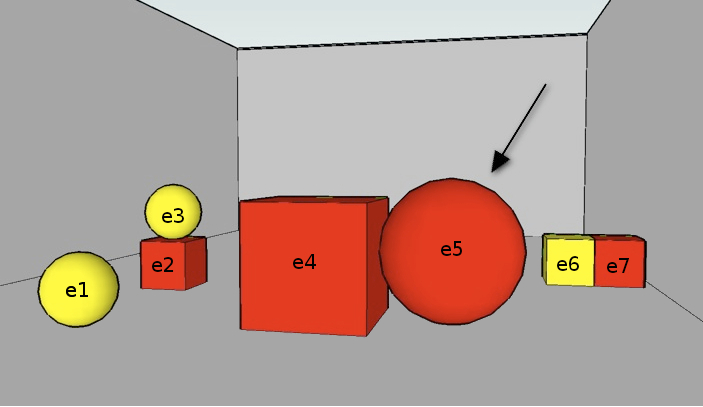
\includegraphics[width=\textwidth]{images/22.jpg}
 % \caption{}\label{GRE3D7-stimulus1-ids-modelo-y-figura}
\end{subfigure}
\begin{subfigure}{.5\textwidth}
  \centering
%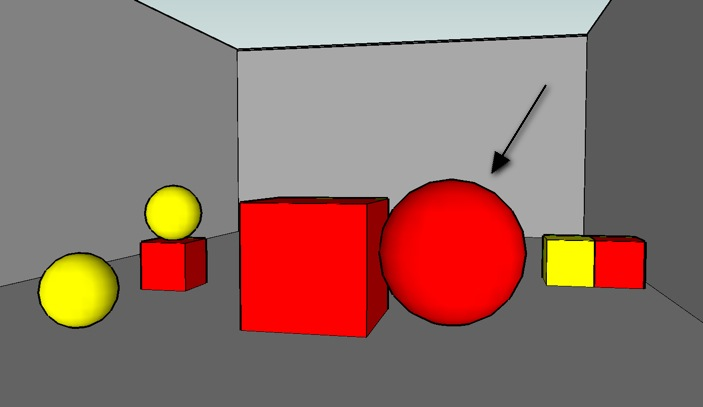
\includegraphics[width=\textwidth]{images/22sinletras.jpg}
%%\caption{Ejemplo de contexto}
%\label{GRE3D7-stimulus1-b}
\vspace*{1cm}
\begin{picture}(250,0)
\put(0,-50){\begin{tikzpicture}
  [
    n/.style={circle,draw,inner sep=1.5pt,node distance=1.5cm},
		 aArrow/.style={->, >=stealth, semithick, shorten <= 1pt, shorten >= 1pt},
  ]
 \node[n,label=below:{
    \relsize{-2}$\begin{array}{c}
      \nSmall\\[-3pt] 
      \nYellow \\[-3pt] 
      \nBall\end{array}$}] (a) {$e_1$};
 \node[n,label=below:{
    \relsize{-2}$\begin{array}{c}     
      \nSmall\\[-3pt] 
      \nRed\\[-3pt] 
      \nCube\end{array}$}, right of=a] (b) {$e_2$};
 \node[n,label=above:{
    \relsize{-2}$\begin{array}{c}     
      \nSmall\\[-3pt] 
      \nYellow\\[-3pt] 
      \nBall\end{array}$}, above of=b] (c) {$e_3$};
 \node[n,label=below:{
    \relsize{-2}$\begin{array}{c}
      \nLarge\\[-3pt] 
      \nRed\\[-3pt] 
      \nCube\end{array}$}, right of=b] (d) {$e_4$};
 \node[n,label=below:{
    \relsize{-2}$\begin{array}{c}
      \nLarge\\[-3pt] 
      \nRed\\[-3pt] 
      \nBall\end{array}$}, right of=d] (e) {$e_5$};
 \node[n,label=below:{
    \relsize{-2}$\begin{array}{c}
      \nSmall\\[-3pt] 
      \nYellow\\[-3pt] 
      \nCube\end{array}$}, right of=e] (f) {$e_6$};
 \node[n,label=below:{
    \relsize{-2}$\begin{array}{c}
      \nSmall\\[-3pt]
      \nRed\\[-3pt] 
      \nCube\end{array}$},  right of=f] (g) {$e_7$};
 \draw [aArrow,bend right=40] (b) to node[auto,swap]{\relsize{-3}$\nBelow$} (c);
 \draw [aArrow,bend right=40] (c) to node[auto,swap]{\relsize{-3}$\nOntop$} (b);
 \draw [aArrow,bend right=40] (d) to node[auto,swap]{\relsize{-3}$\nLeftof$} (e);
 \draw [aArrow,bend right=40] (e) to node[auto,swap]{\relsize{-3}$\nRightof$} (d);
 \draw [aArrow,bend right=40] (f) to node[auto,swap]{\relsize{-3}$\nLeftof$} (g);
 \draw [aArrow,bend right=40] (g) to node[auto,swap]{\relsize{-3}$\nRightof$} (f);
 %\draw[dotted] (-0.5,-1.3) rectangle (8,3.1);
 \draw[dotted] (-0.5,-1.5) rectangle (8,3);
 \end{tikzpicture}}
 \end{picture}
 %\end{flushleft}

%\vspace*{2cm} 
 %\caption{}\label{representacion-modelo-y-figura}

\end{subfigure}%
\caption{Modelo que representa a la figura.}
\label{figura-y-modelo}
\end{figure}


El sistema tambi\'en toma como entrada una \textbf{distribuci\'on de probabilidad finita} de las propiedades y relaciones de la signatura del modelo. En lo que sigue nos referiremos a las propiedades y relaciones de un modelo simplemente como relaciones, distinguiendo entre relaciones unarias (propiedades) o relaciones binarias (relaciones) cuando sea necesario. La distribuci\'on de probabilidades Rs, es una lista de pares de tuplas (R, R.\puse) que vinculan a cada relaci\'on R a una cierta probabilidad de uso R.\puse\ ordenada de mayor a menor por \puse\. La distribuci\'on de probabilidad para el modelo del ejemplo se ilustra en la Tabla \ref{probabilidades-escena}.  Los algoritmos descriptos en el Cap\'itulo \ref{sec:seleccion} y en el Cap\'itulo \ref{sec:intro_logica} procesan las relaciones unarias y las relaciones binarias de forma diferente. Adem\'as, en general prefieren usar primero las relaciones unarias y s\'olo recurrir a las binarias en caso de que sea necesario. Como se ha observado previamente en trabajo emp\'irico~\cite{viet:gene11}, hay escenas en las cuales las personas usan relaciones binarias antes que unarias y aunque no sea necesario usarlas. Por lo tanto para uniformizar el tratamiento de todas las relaciones sin importar su aridad el algoritmo modifica el modelo M antes de comenzar transformando todas las relaciones a binarias. Esto se hace agregando un elemento extra \emph{dummy} al modelo que no representa ning\'un objeto de la escena y que se relaciona con todos los objetos que ten\'ian relaciones unarias. Por ejemplo, en la Figura \ref{figura-y-modelo} se codifica el hecho de que $e_1$ es amarillo diciendo que est\'a relacionado con el elemento \emph{dummy} por la relaci\'on binaria \emph{yellow}. 

\begin{table}[H]
\begin{center}
\footnotesize{
\begin{tabular} {  l c c c c c c c c c }
\hline
%\multicolumn{1}{c}{}
%&\multicolumn{1}{c}{Domain}
%&\multicolumn{3}{c}{Descriptions}\\

R				&{\it ball}			& {\it cube}	& {\it red}	  & {\it large} & {\it ontop} & {\it yellow} & {\it small} & {\it rightof} & {\it leftof}   \\
\hline
R.\puse	& 1.0			& 1.0		& 0.978	& 0.257 & 0.178 & 0.15   & 0.107 & 0.007& 0 \\
\hline

\end{tabular}
}
\end{center}
\vspace*{-.5cm} 
\caption{Distribuci\'on de probabilidad de las propiedades y relaciones de la figura de ejemplo.}\label{probabilidades-escena}

\end{table}
%esfera 1.0, \\
%cube 1.0,\\
%rojo 0.978,\\ 
%large 0.257,\\ 
%ontop 0.178,\\ 
%yellow 0.15,\\
%peque\~no 0.107,\\ 
%izquierda 0.007,\\
%arriba 0.007, \\
%derecha 0, \\
%leftof 0, \\
%a-la-der-de 0, \\
%belowof 0\\

Sea $\REL$ es el
conjunto de todos los s\'imbolos de relaci\'on en el modelo (es decir, la~\emph{signatura} del modelo), entonces podemos decir que Rs $\in (\REL \times [0,1])^*$. En la pr\'oxima secci\'on explicaremos como obtener estas probabilidades que el algoritmo toma como input.

Como explicamos en el Cap\'itulo \ref{sec:intro_logica}, la salida el algoritmo es lo que se llaman las $\mathcal {L}$-clases (clases de la l\'ogica $\mathcal {L}$) de semejanza del modelo de entrada $\gM $. Intuitivamente, si dos elementos en el modelo pertenecen a la misma $\mathcal {L}$-clase de semejanza, entonces el lenguaje~$\mathcal {L}$ no es lo suficientemente expresivo para diferenciarlos (es decir, no hay una f\'ormula en~$\mathcal {L }$ que pueda distinguirlos). Cada  $\mathcal {L}$ clase va acompa\~nada de un conjunto de f\'ormulas cuyas interpretaciones en el modelo de input coinciden con la $\mathcal {L}$-clase. Estas f\'ormulas son las expresiones referenciales que referencian a los elementos de la $\mathcal {L}$-clase. Si alguna $\mathcal {L}$-clase coincide con el conjunto target, el algoritmo termina, e identifica la f\'ormula cuya extensi\'on es igual al target como una ER del target. Como el algoritmo es no determin\'istico el ranking que ERs de la salida se genera ejecutando el algoritmo un n\'umero n de veces. Cada ER generada tiene asociada una probabilidad calculada como una combinaci\'on de los \puse de las relaciones que contiene la ER. El ranking de ERs se genera ordenando las ERs de acuerdo a la frecuencia con la cual el algoritmo la genera, la cual se correlaciona con la probabilidad antes mencionada.

La salida del algoritmo es un conjunto de f\'ormulas y sus interpretaciones en el modelo (que ser\'a ER de un target singleton, si la interpretaci\'on de la f\'ormula contiene s\'olo 1 objeto) de los elementos del modelo. Si al terminar el algoritmo la interpretaci\'on de cada f\'ormula tiene un s\'olo elemento, tenemos una ER que identifica al elemento, para cada elemento del modelo. 

\section{Probabilidades de uso}
\label{sec:learning}

En el secci\'on anterior hemos comentado que el algoritmo supone que para cada relaci\'on R del modelo se tiene una probabilidad de uso R.\puse. En esta secci\'on, explicamos c\'omo es posible obtener estas probabilidades de uso. Como dijimos, nuestro algoritmo es no-determinista: en 2 ejecuciones podr\'ia dar diferentes ERs para el mismo target y la misma lista de probabilidades de uso. Las probabilidades de uso son el motor y gu\'ian este no-determinismo. En la Secci\'on \ref{sec:algoritmo_probabilistico} explicamos c\'omo se dise\~n\'o esta caracter\'istica en el algoritmo. Luego en el Cap\'itulo \ref{sec:evaluacion} veremos como las probabilidades de uso calculadas como se muestran en este cap\'itulo, nos dan un ranking de ERs, que se aproxima a la distribuci\'on de frecuencia de ERs encontradas en corpora.


En el resto de esta secci\'on describimos c\'omo obtener la distribuci\'on de probabilidades finita de las relaciones de la signatura del modelo de entrada. Primero explicamos c\'omo calcularlas en el caso de tener corpus disponible para la escena. Luego generalizamos nuestro enfoque al caso de tener que generar ERs para una escena no vista antes usando t\'ecnicas de aprendizaje autom\'atico.  

%\begin{figure}[H]
%\centering
%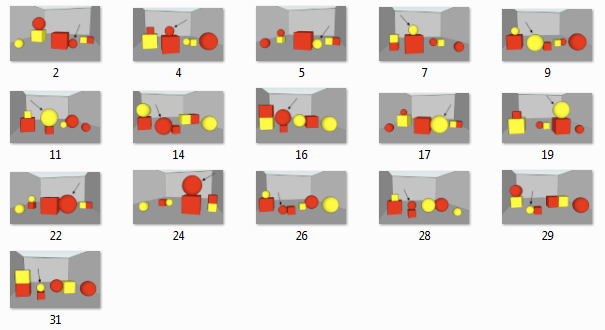
\includegraphics[width=1\textwidth]{images/rojo-amarillo.png}
%\caption{Im\'agenes del \textit{GRE3D7} parte rojo y amarillo}
%\label{rojo-amarillo}
%\end{figure}

\subsection{Calculando \puse\ cuando hay disponible un corpus para la escena considerada}
\label{sec:learning-corpus}

Supongamos que queremos generar autom\'aticamente una ER para el target $t$ en una
determinada escena, y que tenemos disponible un corpus $C$ de ERs de $t$
en esa escena (esto es exactamente el tipo de informaci\'on que encontramos en el
\textit{GRE3D7} corpus \textit{y en el TUNA-corpus}).

En la Figura \ref{verde-azul} se muestran las escenas mostradas a los participantes del corpus \textit{GRE3D7} introducido en la Secci\'on \ref{sec:corpusGRE}, esta parte incluye s\'olo las escenas verde y azules. El corpus contiene otra parte similar con colores rojo y amarillo.

\begin{figure}[H]
\centering
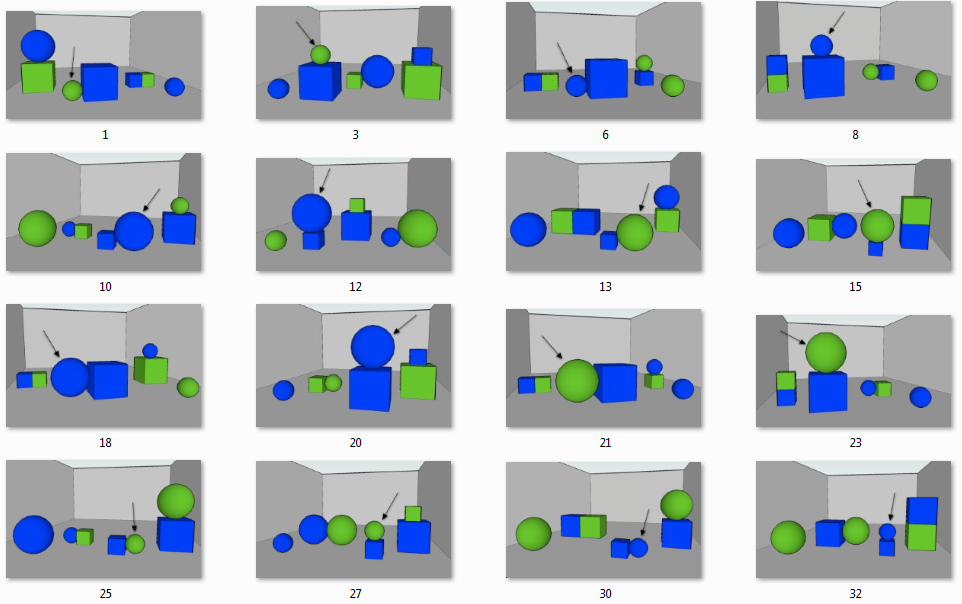
\includegraphics[width=1\textwidth]{images/corpusVerdeAzul.png}
%\vspace{-0.5}
\caption{Im\'agenes del \textit{GRE3D7} parte azul y verde.}
\label{verde-azul}
\end{figure}

El corpus tiene para cada imagen 140 ERs dadas por personas. La Figura \ref{fig4-4} muestra una escena y las distintas ERs que aparecieron en el corpus para esa escena.
\begin{figure}[H]
\begin{minipage}[b]{0.5\linewidth}
\centering
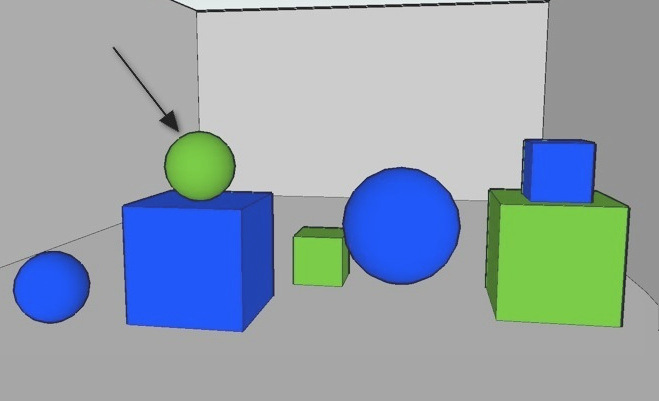
\includegraphics[width=\textwidth]{images/3.jpg}
%\vspace*{1cm}
%\caption{Contexto 3 del GRE3D7}
\end{minipage}
\hspace*{1cm}
\begin{minipage}[b]{0.5\linewidth}
\footnotesize{
{\it green ball} \\
{\it small green ball}  \\
{\it small green ball on top of large red cube} \\
{\it green ball on top of blue cube}\\
{\it green ball on top of large blue cube} \\
{\it small green ball on top of blue cube}  \\
{\it ball on top of cube} \\
{\it small green ball on top of red large left cube}  \\
{\it small ball on top of cube large}  \\
{\it top green ball}   \\
{\it small ball on top of cube } \\
{\it green ball on top of cube }

%green ball \\
%small green ball  \\
%small green ball on-top red large cube \\
%green ball on-top blue cube\\
%green ball on-top large blue cube \\
%small green ball on-top blue cube  \\
%ball on-top cube \\
%small green ball on-top red large left cube  \\
%small ball on-top cube large  \\
%top green ball   \\
%small ball on-top cube  \\
%green ball on-top cube  \\
}
\end{minipage}
\caption{ERs dadas por las personas que completaron el experimento del corpus \textit{GRE3D7} para el contexto de la imagen.}\label{fig4-4}
\end{figure}
Las ERs dadas en Figura \ref{fig4-4} son las ERs diferentes que est\'an en el corpus para el contexto mostrado en la misma figura. Viendo esas ERs, uno podr\'ia imaginarse que no son las del corpus mismo, ya que diferentes personas normalmente usan distintas palabras para nombrar al mismo objeto, distintas frases, distinto orden de las palabras, s\'i es verdad, este corpus ya ha sido procesado para filtrar todas esas cosas, dejar un vocabulario com\'un a todas las ERs, si bien es verdad que con eso perdemos informaci\'on por ejemplo de la realizaci\'on particular que hizo una persona, pero ganamos en poder agrupar las ERs por la informaci\'on que la persona incluy\'o, en la etapa de selecci\'on de contenido de la ER. Si quisieramos partir de un corpus con las ERs tal cual dieron las personas, tendr\'iamos que realizar los siguientes pasos a fin de unificar el vocabulario:

Antes de dar la metodolog\'ia para calcular las probabilidades de uso, explicaremos qu\'e hacer con un corpus de ERs para tener unificado el vocabulario, recordemos que el objetivo de la tesis se centra en la selecci\'on de contenidos de las ERs y por ello, no vamos a prestar atenci\'on a la realizaci\'on particular que di\'o cada persona de la ER. 

\begin{enumerate}
\item \textbf{Tokenizar} las expresiones referenciales y llamar al conjunto de palabras distintas
 $Pal$. En particular, las expresiones de varias palabras como {\it arriba de}, {\it encima de}
  deben ser igualadas a una \'unica palabra que signifique lo mismo, digamos \emph{ontop}.

\item \textbf{Eliminar hiper\'onimos} de $Pal$. Por ejemplo, si ambos \emph{cube} y
  \emph{cosa} aparecen en $Pal$ para nombrar la misma cosa, eliminar \emph{cosa}, ya que \emph{cube} es m\'as espec\'ifico.

\item \textbf{Normalizar sin\'onimos} si el conjunto de palabras obtenidas en los pasos anteriores contiene
  sin\'onimos hay que normalizarlos con un representante de la clase. Por ejemplo, las palabras \emph{chico}
  y \emph{peque\~no} son ambas representadas por la palabra \emph{small}.

\item \textbf{Llamar $\REL$} al conjunto resultante, de la etapa anterior; que ser\'a la signatura del modelo $\gM$ que utilizar\'a el algoritmo.

\item \textbf{Definir $\gM$} para cada escena, tal que la interpretaci\'on
 $\interp {\cdot}$ asegure de que todas las ERs encontradas en el corpus sean ERs en
  el modelo. Por ejemplo, las ERs de \ref{fig4-4} deben denotar el target se\~nalado en la figura, siendo el modelo 
$\gM$ considerado el representado en Figura~\ref{fig4-5}.
%GRE3D7-stimulus-cap2
\item \textbf{Calcular R.\puse\ }para cada R$\in \REL$ utilizando la siguiente f\'ormula: Si
  hay muchas ERs para cada escena (como es el caso del corpus \textit{GRE3D7}) $R.\puse\ = \#ERs que tienen R /\#ERs en el corpus$
    
  o asignamos 1 a R.\puse \ si R esta en ER, asignamos 0 en caso contrario (como es el caso del corpus TUNA).
\end{enumerate}

En el caso del corpus \textit{GRE3D7} el vocabulario unificado y la signatura del modelo es 
$\REL = \{ball, cube, large, small, green, red, yellow, blue, right, left, top, center, rightof, leftof, ontop,\\ 
bellow\} $

En lo que sigue daremos la definici\'on de regresi\'on lineal que es lo que usaremos para estimar las probabilidades de uso \puse\ de las palabras que le daremos al algoritmo, y luego daremos un ejemplo de c\'omo calculamos las probabilidades de uso para una figura particular del \textit{GRE3D7}.

La \textbf{regresi\'on lineal} es un modelo matem\'atico usado para aproximar la relaci\'on de dependencia entre una variable dependiente Y, las variables independientes $X_i$ y un t\'ermino aleatorio $\varepsilon$. Este modelo puede ser expresado como:

    $Y_t = \beta_0 + \beta_1 X_1 + \beta_2 X_2 + \cdots +\beta_p X_p + \varepsilon$

donde:

    $Y_t$: variable dependiente, explicada o regresando.
    $X_1$, $X_2$, $\cdots$, $X_p$ : variables explicativas, independientes o regresores.
    $\beta_0$,$\beta_1$,$\beta_2$,$\cdots$,$\beta_p$ : par\'ametros, miden la influencia que las variables explicativas tienen sobre Y.

donde $\beta_0$ es la intersecci\'on o t\'ermino {\it constante}, las $\beta_i$ \ (i > 0) son los par\'ametros respectivos a cada variable independiente, y $p$ es el n\'umero de par\'ametros independientes a tener en cuenta en la regresi\'on.

Tomaremos la parte azul y verde del corpus \textit{GRE3D7} mostrado en la Figura \ref{verde-azul}, para aprender las probabilidades de uso de cada palabra de las ERs que dieron las personas, y as\'i darnos una idea de como es la distribuci\'on del uso de las palabras del conjunto $REL$ en el corpus.

Hemos seleccionado algunas propiedades, las cuales las sacamos autom\'aticamente del XML del corpus, nuestro objetivo principal, en esta secci\'on, es conseguir un conjunto de propiedades que son las variables $X_i$ que le daremos al m\'etodo de regresi\'on lineal para calcular la dependencia o independencia de la probabilidad de uso \puse\ de cada palabra con respecto a esas propiedades.

\begin{small}
\begin{table}[H]
\begin{center}
\begin{tabular}{|l|p{10cm}|}
\hline
target-tiene & cuando el elemento target tiene la propiedad. \\
\#rel-prop & n\'umero de propiedades y relaciones que el target tiene.\\
\#rel & n\'umero de relaciones que el target tiene. \\
landmark-tiene & cuando un landmark del target tiene la propiedad, un objeto es un landmark si tiene una relaci\'on directa en el modelo, con el target (lo usamos para el \textit{GRE3D7}).\\
location-has & cuando la RE puede usar la ubicaci\'on del target en la figura (esto se hizo porque el TUNA corpus tiene algunas ER donde se le dijo a la gente que pod\'ian usar la localizaci\'on del objeto).\\
discriminaci\'on (disc) & calculada como 1 sobre el n\'umero de objetos en el modelo que tienen la propiedad.  \\
adj-target-tiene & calculada como la cantidad de adjetivos que la ER contiene.\\
\hline
\end{tabular}
\caption{Caracter\'isticas usadas para conseguir f\'ormulas con regresi\'on lineal que nos den una idea de la probabilidad de uso de cada palabra.} 
\label{features}
\end{center}
\end{table}
\end{small}

El procedimiento entonces fue el siguiente:
Creamos un archivo por cada palabra del vocabulario, es decir por ejemplo para ball, cube, small, red, etc. En cada l\'inea del archivo 
se escribieron la lista de propiedades nombradas anteriormente en la Tabla \ref{features}, para la imagen considerada. Como en total 
fueron consideradas 16 im\'agenes, la primer l\'inea contenia la lista de propiedades calculadas desde el corpus de la Figura 1 del \textit{GRE3D7}, 
la segunda l\'inea del de la Figura 3, y as\'i sucesivamente para todas las figuras que se muestran en la Figura \ref{verde-azul}. 
Cada archivo (uno por cada propiedad o relaci\'on del vocabulario) fue analizado con la funci\'on de regresi\'on lineal del paquete WEKA 
\cite{Hall:WEK09}, que tiene una colecci\'on de herrramientas para aprendizaje autom\'atico.

En la Tabla \ref{tabla-linear-regresion-all} se muestran 4 columnas: en la primer columna podemos ver la palabra, 
en la segunda columna est\'a el error promedio dado por regresi\'on lineal, en la tercera columna el error medio 
y en la cuarta la f\'ormula que regresi\'on lineal calcul\'o para la probabilidad de uso de la palabra considerada.

\begin{table}[H]
\begin{center}
\begin{tabular}{|l|c|c|l|}
\hline
Palabra &Error promedio	LR	& Error-PM	& F\'ormula de LR\\
\hline
ball		 &0.0465   &0.0609	  & 0.2894 * disc + 0.7883\\
\hline
cube		 &0.0417	 &0.0531	  &0.49   * disc - 0.0129\\
\hline
\hline
blue		 &0.0353	 &0.0454	  &0.848  * target-tiene + 0.1073\\
\hline
green		 &0.0264	 &0.046	    &0.8722 * target-tiene + 0.0016\\
\hline
\hline
large		 &0.1762	 &0.2378	  &0.5911 * target-tiene + 0.0354\\
\hline
small		 &0.1499	 &0.1755	  &0.3918 * target-tiene + 0.2478 * landmark-tiene -\\
				 &				 &					&0.0913\\
\hline
\hline
leftof  &0.0041	 &0.0094	  &0.0131 * target-tiene +\\
				 &				 &					&0.0253 * adj-target-tiene - 0.0507\\
\hline
ontop	 &0.0706	 &0.1594	  &0.2942 * target-tiene \\
\hline
rightof &0.0029	 &0.0049	  &0.0153 * target-tiene + 0.001\\
\hline
\hline
left		 &0.0068	 &0.0101	  &0.0346 * adj-target-tiene - 0.0653\\
\hline
right		 &0.0079	 &0.0092	  &-0.0118 * disc + 0.0141\\
\hline
top    &0.0099 	 &0.0135		& 0.0069\\
\hline
center	 &0.0023	 &0.0037	  &0.0047 * target-tiene + 0.0047 * adj-target-tiene +\\
				 &				 &					&0.0029 * landmark-tiene - 0.009\\
\hline
\end{tabular}
\caption{F\'ormulas y errores de regresi\'on lineal para la parte del corpus \textit{GRE3D7} que se muestra en la Figura \ref{verde-azul}.}
\label{tabla-linear-regresion-all}
\end{center}
\end{table}

Las palabras {\it red} y {\it yellow} no aparecen en la Tabla \ref{tabla-linear-regresion-all} porque no aparec\'ian en las ERs del corpus de las im\'agenes consideradas (las que conten\'ian colores verdes y azules).

%\textbf{A ESTA TABLA LE FALTAN 3... DEBERIA AGREGARLAS!}

%En la Tabla \ref{tabla-linear-regresion-all} se muestran 4 columnas: en la primer columna podemos ver la palabra, 
%en la segunda columna est\'a el error promedio dado por regresi\'on lineal, en la tercera columna el error medio 
%y en la cuarta la f\'ormula que regresi\'on lineal calcul\'o para la probabilidad de uso de la palabra considerada. 

Podemos ver por ejemplo que {\it ball} tiene una \puse\ alta, es natural ya que en el corpus todos los targets son {\it ball}, como se v\'e en la Figura \ref{verde-azul}, en cambio se puede ver que {\it cube} no es tan alta y depende de la discernibilidad, este n\'umero en la \puse\ debe leerse como la probabilidad de usar {\it cube} en la descripci\'on del landmark. En los casos de {\it blue} y {\it green} el valor de \puse\ depende de si el target es {\it blue} o {\it green}, entonces si el target es {\it blue}, le d\'a un valor alto a {\it blue} y bajo a {\it green} y viceversa, no depende del valor de discernibilidad en el modelo. En la tabla tambi\'en podemos ver que relaciones como {\it small} y {\it large} tienen un error mucho m\'as alto que el resto de las relaciones, esto se debe a que ellas son propiedades vagas. Este tipo de propiedades no son absolutas y dependen del contexto considerado.
Las relaciones {\it ontop}, {\it leftof} y {\it rightof} dependen fuertemente si el target tiene o no esa relaci\'on y en caso de tenerla igualmente la \puse\ no es muy alta, esto indica que en un porcentaje del 30\% por ejemplo se usa {\it ontop} y en menos del 3\% {\it leftof} o {\it rightof}, esta observaci\'on fue reportada en (Viethen, 2011). Una caracter\'istica interesante que vemos y que no fue mencionada en trabajo previo es que tama\~no es m\'as frecuente usado para sobreespecificaci\'on cuando el target y el landmark tienen el mismo tama\~no 
(es usado en ERs sobreespecificadas el 49\% cuando el target y el landmark comparten el tama\~no, y s\'olo el 25\% cuando no lo comparten).

 Utilizamos las ER de $C$
para definir el modelo relacional utilizado por el algoritmo. Entonces 
estimaremos el valor de \puse\ para cada una de las relaciones en el modelo como el
porcentaje en que aparece la relaci\'on en las ER. Es decir,
\begin{equation} \label{eq1}
R.\puse = \frac {\#\mbox{de ERs en $C$ en el que aparece R}} {\#\mbox{de las ER en $C$}}.
\end{equation}

Por ejemplo {\it ball} del ejemplo de la Figura \ref{fig4-4}, apareci\'o en todas las ERs del corpus es decir 140, entonces {\it ball}\puse\=1 ya que 140/140=1, en cambio {\it green} apareci\'o en 137 ERs, entonces {\it green}\puse=0.98 ya que 137/140=0.98.

Esta estimaci\'on es simplista y, por ejemplo, no 
diferencia las propiedades del target y las propiedades de
los landmarks utilizadas en una ER relacional para completar la descripci\'on
del target. Pero es intuitiva y no requiere parsear las ERs para distinguir entre target y landmark. Como vamos a ver
en el Cap\'itulo~\ref{sec:evaluacion} produce ERs naturales
que coinciden con las encontradas en corpora.

Veamos ahora el siguiente ejemplo, el contexto y las ERs del corpus para la escena se muestran en la Figura \ref{fig4-4}. Se muestra en la Figura \ref{fig4-5}, el modelo que representa 
las propiedades y relaciones de los objetos del contexto considerado.

\begin{figure}[H]
\centering
\begin{tikzpicture}
  [
    n/.style={circle,draw,inner sep=3pt,node distance=2cm},
    aArrow/.style={->, >=stealth, semithick, shorten <= 1pt, shorten >= 1pt},
  ]
 \node[n,label=below:{
    \relsize{-1}$\begin{array}{c}
      \nLeft\\[-2pt]
      \nSmall\\[-2pt] 
      \nBlue\\[-2pt]
      \nBall\end{array}$}] (a) {$e_1$};

 \node[n,label=below:{
    \relsize{-1}$\begin{array}{c}
      \nLeft\\[-2pt]
      \nBig\\[-2pt] 
      \nBlue\\[-2pt]
      \nCube\end{array}$}, right of=a] (b) {$e_2$};

 \node[n,label=above:{
    \relsize{-1}$\begin{array}{c}
      \nTop\\[-2pt]      
			\nLeft\\[-2pt]
      \nSmall\\[-2pt]      
			\nGreen\\[-2pt]
      \nBall\end{array}$}, above of=b] (c) {$e_3$};

 \node[n,label=below:{
    \relsize{-1}$\begin{array}{c}
      \nSmall\\[-2pt] 
      \nGreen\\[-2pt] 
      \nCube\end{array}$}, right of=b] (d) {$e_4$};

 \node[n,label=below:{
    \relsize{-1}$\begin{array}{c}
      \nBig\\[-2pt] 
      \nBlue\\[-2pt] 
      \nBall\end{array}$}, right of=d] (e) {$e_5$};

 \node[n,label=below:{
    \relsize{-1}$\begin{array}{c}
      \nBig\\[-2pt] 
      \nGreen\\[-2pt] 
      \nCube\end{array}$}, right of=e] (f) {$e_6$};

 \node[n,label=above:{
    \relsize{-1}$\begin{array}{c}
      \nTop\\[-2pt]
      \nSmall\\[-2pt]
      \nBlue\\[-2pt]
      \nCube\end{array}$}, above of=f] (g) {$e_7$};

 \draw [aArrow,bend right=90] (b) to node[auto,swap]{\relsize{-1}$\nBelow$} (c);
 \draw [aArrow,bend right=90] (c) to node[auto,swap]{\relsize{-1}$\nOntop$} (b);

 \draw [aArrow,bend right=30] (d) to node[auto,swap]{\relsize{-1}$\nLeftof$} (e);
 \draw [aArrow,bend right=30] (e) to node[auto,swap]{\relsize{-1}$\nRightof$} (d);

 \draw [aArrow,bend right=90] (f) to node[auto,swap]{\relsize{-1}$\nBelow$} (g);
 \draw [aArrow,bend right=90] (g) to node[auto,swap]{\relsize{-1}$\nOntop$} (f);
\draw[dotted] (-0.5,-2.4) rectangle (10,4.7);
 %\draw[dotted] (-.65,-1.2) rectangle (7.1,2.1);

 \end{tikzpicture}
\vspace*{-.4cm}\caption{Representaci\'on de las propiedades y relaciones, como un grafo etiquetado, del contexto de la Figura \ref{fig4-4}.}
\label{fig4-5}
\end{figure}

Las ERs, cantidad de ocurrencias y porcentaje del corpus para de la Figura~\ref{fig4-4} se muestran en la Tabla~\ref{corpus-distribution}, la signatura resultante y su \puse\ asociado figuran en las dos primeras columnas de la Tabla~\ref{probability-of-use}.\\

\begin{table}[h!]
\begin{center}
\begin{tabular}{|l|c|c|}
\hline
Expresiones Referenciales & Cantidad de ocurrencias & Porcentaje \\
\hline

green ball & 91 & 65.00\% \\
small green ball   & 23 & 16.43\% \\
small green ball on-top red large cube & 8 & 5.71\% \\
green ball on-top blue cube & 5 & 3.57\% \\
green ball on-top large blue cube & 5 & 3.57\% \\
small green ball on-top blue cube & 2 & 1.43\% \\
ball on-top cube & 1 & 0.71\% \\
small green ball on-top red large left cube  & 1 & 0.71\% \\
small ball on-top large cube & 1 & 0.71\% \\
top green ball  & 1 & 0.71\% \\
small ball on-top cube & 1 & 0.71\% \\
green ball on-top cube & 1 & 0.71\% \\

\hline
\end{tabular}
\caption{Sem\'antica de las expresiones referenciales producidas por las personas para la Figura~\ref{fig4-4}.}\label{corpus-distribution}
\end{center}
\end{table}

Observe que los valores R.\puse\ obtenidos de esta manera deben ser
interpretados como la probabilidad de utilizar R para describir el target en
modelo de $\gM $, y podr\'{i}amos argumentar que se correlacionan con la
 saliencia de R para el target y su modelo. Por esa raz\'on, por ejemplo, el
valor de \emph{ball}.\puse\ es 1, mientras que el valor de
\emph{cube}.\puse\ es 0.178. \\

Estas probabilidades no ser\'an \'utiles
para describir los diferentes targets en diferentes escenas. Veremos c\'omo se
pueden utilizarlas para obtener valores para los nuevos targets y escenas utilizando un
enfoque de aprendizaje autom\'atico en la siguiente secci\'on. Como mostramos en el Cap\'itulo~\ref{sec:evaluacion} el algoritmo genera ER
con una distribuci\'on que coincide con la encontrada en el corpus e incluso las ERs generadas por el algoritmo que no se encontraron
en el corpus son naturales.



\subsection{Calculando \puse\ para el target para escenas sin corpus } 
\label{subsec:learning}

%If there is no corpora that describes the target we can estimate the
%\puse~from corpora on a different scenes in the same domain.
%
%We use simple features to obtain the function, all the features can be
%extracted automatically from the relational model and are listed in


Si no hay corpus de expresiones referenciales que describen el target, se puede estimar la \puse~a partir de corpus de
diferentes escenas en el mismo dominio.
Usamos caracter\'isticas simples para obtener una funci\'on que nos dar\'a la probabilidad de cada palabra en el nuevo modelo, todas las caracter\'isticas se pueden extraer de forma autom\'atica desde el modelo relacional y se enumeran en la Tabla~\ref{features}.

\begin{itemize}
\item target-tiene 1 cuando el elemento target tiene la propiedad o sino 0. 
\item \#rel-prop n\'umero relaciones unarias y binarias que el target tiene.
\item \#rel  n\'umero de relaciones binarias que el target tiene. 
\item landmark-tiene cuando un landmark del target tiene la propiedad.
%location-has & cuando la RE puede usar la ubicaci\'on del target en la figura (esto se hizo porque el TUNA corpus tiene algunas ER donde se le dijo a la gente que pod\'ian usar la localizaci\'on del objeto).\\
\item disc calculada como 1 sobre el n\'umero de objetos en el modelo que tienen la propiedad.  
\item adj-target-tiene calculada como la cantidad de adjetivos que la ER contiene.
\end{itemize}

En el caso del \textit{GRE3D7} usamos la parte verde-azul, es decir todas las im\'agenes que tienen colores verde y azul, para acotar el problema, asumiendo que la otra parte dar\'ia algo similar. En la Figura \ref{verde-azul} se muestran los contextos considerados.

Para hacer el aprendizaje, separamos 1 contexto al que llamamos testing, y todos los dem\'as de entrenamiento. Por ejemplo para aprender \puse\ del contexto 13, se usaron los contextos: 1, 3, 6, 8, 10, 12, 15, 18, 20, 21, 23, 25, 27, 30 y 32. Y as\'i sucesivamente para los dem\'as contextos.

Nuestro conjunto de caracter\'{i}sticas es intencionadamente simplista con el fin de que sea
independiente de dominio. Como resultado hay algunas relaciones complejas
entre las caracter\'{i}sticas de las escenas que no es capaz de
capturar. La caracter\'{i}stica m\'as importante del dominio \textit{GRE3D7}
que no somos capaces de aprender, y tiene un impacto en nuestro desempe\~no, es que
las propiedades de tama\~no (es decir, small y large) se utilizan mucho
m\'as cuando el target no puede ser identificado s\'olo con las propiedades taxon\'omicas absolutas 
(verde y azul) y (ball y cube). En otras palabras, en el corpus \textit{GRE3D7} se utiliza el tama\~no con m\'as frecuencia (90,2 \%)
cuando la ER resultante no es sobreespecificada y cuando si es sobreespecificada el (34 \%). 
Puede que no sea posible aprender esta caracter\'{i}stica de los
datos del \textit{GRE3D7} ya que incluso con las funciones que dependen de dominio definidos
en~\cite[Cap\'{i}tulo 6] {viet:gene11}, no pod\'{i}a ser aprendido por \'arboles decisi\'on. 
Como resultado podemos ver en la Tabla~\ref{probability-of-use} de la Figura 13, el valor estimado para 
\emph{large} no est\'a cerca de la
valor calculado a partir de corpus. En el caso del TUNA-corpus
  mostramos que no podemos aprender la dependencia de la dimensi\'on-X y
  dimensi\'on-y, es decir, cuando una persona a\~nade dimensi\'on-x es altamente
  probable que incluya la dimensi\'on-y en su expresi\'on referencial.

\begin{figure}[ht]
\begin{minipage}[b]{0.5\linewidth}
\centering
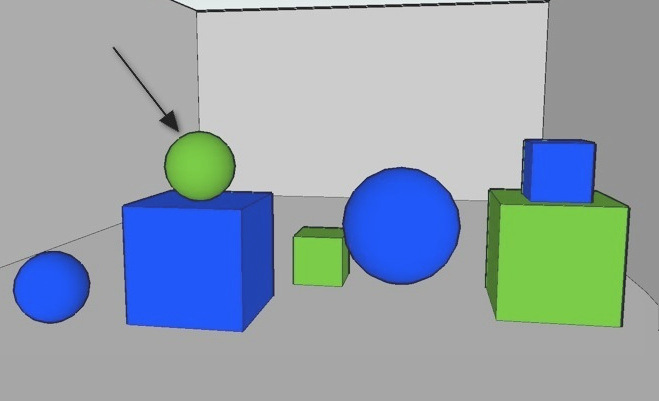
\includegraphics[width=\textwidth]{images/3.jpg}
%\vspace*{1cm}
\caption{Contexto 3 del \textit{GRE3D7}.}
\label{GRE3D7-stimulus-3}
\end{minipage}
%\hspace*{-0.35cm}
\begin{minipage}[b]{0.5\linewidth}
\centering
%\begin{figure}[ht]
%\begin{center}
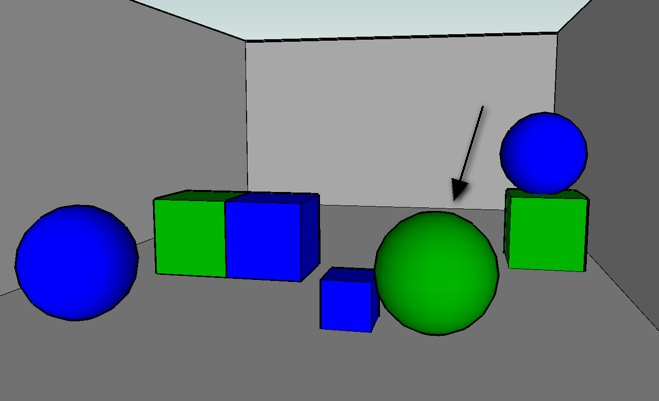
\includegraphics[width=\textwidth]{images/13.jpg}
\caption{Contexto 13 del \textit{GRE3D7}.}
\label{GRE3D7-stimulus-13}
\end{minipage}
\end{figure}

\begin{table}[h!]
\begin{center}
\begin{tabular}{|l|c|c|c|c|}
\hline
%Palabra &  \puse 				 & \puse\ Aprendida 			   & \puse\ & \puse\  Aprendida \\
Palabra & \puse\ Figura \ref{GRE3D7-stimulus-3}   & \puse\ aprendida \ref{GRE3D7-stimulus-3} & \puse\ Figura \ref{GRE3D7-stimulus-13} & \puse\ aprendida \ref{GRE3D7-stimulus-13}  \\
\hline
ball & 1.0 & 1.0 & 1.0 & 1.0 \\
cube & 1.0 & 1.0 & 1.0 & 1.0 \\
green & 0.978 & 0.993 & 1.0 & 0.9875 \\
small & 0.257 & 0.346 & 0.0428 & 0.1993 \\
ontop & 0.178 & 0.179 & 0 & 0\\ 
blue & 0.15 & 0.124 & 0.064 & 0.1353 \\
large & 0.107 & 0.03 & 0.307 & 0.7378 \\
left & 0.007 & 0.002 & 0 & 0.0024 \\
top & 0.007 & 0 & 0 & 0 \\
right & 0 & 0.001 & 0.064 & 0.0005 \\
leftof & 0 & 0 & 0 & 0 \\
rightof & 0 & 0 & 0.064 & 0.1023 \\
belowof & 0 & 0 & 0 & 0 \\
\hline
\end{tabular}
\caption{Probabilidades de uso de las palabras del corpus \textit{GRE3D7} para las Figuras \ref{GRE3D7-stimulus-3} y \ref{GRE3D7-stimulus-13}.} 
\label{probability-of-use}
\end{center}
\end{table}


\begin{table}[h!]
\begin{center}
\begin{tabular}{|l|c|c|}
\hline
%Palabra &  \puse 				 & \puse\ Aprendida 			   & \puse\ & \puse\  Aprendida \\
Palabra & \puse\ Figura \ref{GRE3D7-stimulus-3}   &  \puse\ Figura \ref{GRE3D7-stimulus-13} \\
\hline
ball & 1.0 & 1.0  \\
cube & 1.0 & 1.0  \\
green & 0.978 &  1.0  \\
small & 0.257 & 0.0428  \\
ontop & 0.178  & 0 \\ 
blue & 0.15 & 0.064  \\
large & 0.107  & 0.307  \\
left & 0.007  & 0  \\
top & 0.007  & 0 \\
right & 0  & 0.064  \\
leftof & 0  & 0  \\
rightof & 0  & 0.064  \\
belowof & 0  & 0 \\
\hline
\end{tabular}
\caption{Probabilidades de uso de las palabras del corpus \textit{GRE3D7} para las Figuras \ref{GRE3D7-stimulus-3} y \ref{GRE3D7-stimulus-13}.} 
\label{probability-of-use}
\end{center}
\end{table}


\begin{table}[h!]
\begin{center}
\begin{tabular}{|l|c|c|}
\hline
%Palabra &  \puse 				 & \puse\ Aprendida 			   & \puse\ & \puse\  Aprendida \\
Palabra &  \puse\ aprendida \ref{GRE3D7-stimulus-3} & \puse\ aprendida \ref{GRE3D7-stimulus-13}  \\
\hline
ball &  1.0 & 1.0 \\
cube &  1.0 & 1.0 \\
green &  0.993 & 0.9875 \\
small &  0.346 & 0.1993 \\
ontop &  0.179 & 0\\ 
blue &  0.124  & 0.1353 \\
large &  0.03  & 0.7378 \\
left &  0.002  & 0.0024 \\
top &  0 & 0 \\
right &  0.001 & 0.0005 \\
leftof &  0 &  0 \\
rightof & 0 &  0.1023 \\
belowof & 0 &  0 \\
\hline
\end{tabular}
\caption{Probabilidades de uso aprendidas para las Figuras \ref{GRE3D7-stimulus-3} y \ref{GRE3D7-stimulus-13}.} 
\label{probability-of-use}
\end{center}
\end{table}


El aprendizaje se realiza con el kit de herramientas de aprendizaje autom\'atico
WEKA~\cite{Hall:WEK09}, entrenando con todas las escenas menos una (para la que estamos aprendiendo) se realiz\'o para el corpus \textit{GRE3D7} y el \textit{TUNA-corpus}. Un ejemplo del contenido de los archivos XML del \textit{TUNA-corpus} se muestra en el Ap\'endice \ref{archivos-xml-tuna}. El corpus cuenta con im\'agenes generadas aleatoriamente, por lo tanto las im\'agenes que se muestran en esta tesis, pueden no ser exactamente como las im\'agenes mostradas a los participantes.

Un ejemplo de archivo de los que toma WEKA como input se d\'a en el Ap\'endice \ref{archivos-arff-blue}. Este archivo corresponde a propiedad {\it blue} 
de la parte muebles del \textit{TUNA-corpus}. Utilizamos regresi\'on lineal para aprender la funci\'on de
\puse\ para cada palabra en la signatura. Para una escena determinada, reemplazamos
las variables de la funci\'on obtenida por los valores de las caracter\'{i}sticas
de la escena que queremos describir.

La regresi\'on lineal nos permite aprender caracter\'{i}sticas interesantes
 del dominio. Para empezar, se aprenden hechos conocidos
como que un determinado {\it color} aparezca en la ER depende en gran medida de si el
target es de ese color, y que no depende de su
poder de discriminaci\'on en el modelo. Por otra parte, vimos que la relaci\'on {\it ontop}
 se utiliza con m\'as frecuencia que las relaciones horizontales
({it right}, {it left}) lo que confirma un hallazgo previo informado
en~\cite{viet:gene11}. Por \'ultimo, vimos en el
\textit{GRE3D7} corpus (que no fue reportado por el trabajo anterior), se utiliza el tama\~no
m\'as frecuentemente de una manera sobreespecificada cuando el
target y el landmark comparten el tama\~no. El {\it tama\~no} fue utilizado en las ER de manera sobreespecificada en el 49 \% de
las descripciones de escenas en las que el target y el landmark compart\'ian el tama\~no,
y el 25 \% cuando target y el landmark no lo compart\'ian. Esto puede explicarse por la observaci\'on de que si landmark y el target comparten una propiedad, esta propiedad es m\'as relevante.

\section{El algoritmo probabil\'istico}
\label{sec:algoritmo_probabilistico}
Antes de empezar explicando el algoritmo, daremos algunos conceptos de teor\'ia de modelos necesarios para entenderlo.

Una \textbf{f\'ormula} corresponde a una descripci\'on de uno o m\'as elementos del contexto y puede ser o no una ER dependiendo de 
si su interpretaci\'on coincide o no con el target. Por ejemplo la interpretaci\'on de la f\'ormula \texttt{ball} son todas las esferas 
del contexto. En el contexto de la Figura \ref{figura-y-modelo} ser\'ian: $e_1$, $e_3$ y $e_5$  as\'i como $\interp{\texttt{ball} \land \texttt{yellow}}$ es: $e_1$ y $e_3$.
Como dijimos anteriormente la \textbf{interpretaci\'on de una f\'ormula} es el conjunto de elementos que satisfacen la f\'ormula. A la interpretaci\'on de una f\'ormula tambi\'en la llamaremos \textbf{clase}.

Decimos que una f\'ormula $\exists.R. \phi$ es \textbf{informativa} con respecto a otra f\'ormula $\gamma$ cuando la interpretaci\'on de la conjunci\'on de las dos f\'ormulas ($\exists.R. \phi \land \gamma$) contiene menos elementos que la interpretaci\'on de $\gamma$. Por ejemplo si tenemos la f\'ormula \texttt{ball} y 
queremos saber si \texttt{red} es informativa con respecto a \texttt{ball} para el modelo de la Figura vemos que, s\'i lo es, ya que $e_5$ es una \texttt{esfera roja} y existen otras esferas que no son rojas,
 es decir \texttt{red} divide el conjunto de esferas, por lo tanto es informativa. Si un algoritmo permite agregar f\'ormulas no informativas a las expresiones referenciales, entonces podr\'a generar ERs sobreespecificadas.

Una f\'ormula es \textbf{subsumida} si ya tenemos otras f\'ormulas en RE con m\'as informaci\'on que cubren todo el conjunto de objetos que 
la f\'ormula cubr\'ia. Por ejemplo, $\top$ que es la f\'ormula a la cual todos los objetos pertenecen, ser\'a subsumida cuando se agreguen 
las f\'ormulas \texttt{ball} y \texttt{cube} ya que todos los elementos de la Figura \ref{figura-y-modelo} son o esferas o cubos, 
es decir ya tenemos informaci\'on m\'as precisa de los objetos que $\top$. Formalmente $\interp{\top}$ = \{$e_1$,$e_2$,$e_3$,$e_4$,$e_5$,$e_6$, $e_7$\}, y los conjuntos \interp{\texttt{ball}}=\{$e_1$,$e_3$,$e_5$\} y la \interp{\texttt{cube}}=\{$e_2$,$e_4$,$e_6$,$e_7$\}. La uni\'on de los conjuntos $\interp{\texttt{ball}}$ y $\interp{\texttt{cube}}$ dan exactamente $\interp{\top}$.

%\textbf{Redundante} es una f\'ormula para la cual ya hay otra f\'ormula la cual tenga los mismos objetos del modelo. Por ejemplo para el 
%contexto de la Figura \ref{figura-y-modelo}, si ya tenemos la f\'ormula \texttt{red ball}, la f\'ormula \texttt{large red ball} es redundante, ya 
%que no agrega informaci\'on porque el conjunto de objetos esferas rojas ya ten\'ia solamente 1 objeto $e_5$. Intuitivamente es redundante cuando no divide a ninguna clase.

\textbf{Trivial} es una f\'ormula para la cual no hay objetos que la satisfagan en el modelo considerado, por ejemplo en el contexto de la 
Figura \ref{figura-y-modelo}, \texttt{large yellow ball} es trivial ya que no hay esferas amarillas grandes en el contexto considerado.

Vamos a utilizar f\'ormulas de el lenguaje de descripci\'on $\el$ de la l\'ogica~\cite{baad:desc03} para describir clases de refinamiento.
Note, sin embargo, que el lenguaje formal utilizado en particular es independiente del algoritmo principal, y diferentes 
funciones add$_{\mathcal {L}}$(R,$\varphi $, \RE) se pueden utilizar en funci\'on del lenguaje en cuesti\'on.
%Para una descripci\'on detallada de $\el$, nos referimos a~\cite{baad:desc03}.

La interpretaci\'on de la f\'ormula de $\el$  $\psi \sqcap \exists $R.$ \varphi$ es el conjunto de todos los elementos que 
satisfagan~$\psi$ y que est\'an relacionados por relaci\'on R con alg\'un elemento que satisface $\varphi $.
Por ejemplo, la interpretaci\'on de la f\'ormula \texttt{ball}$\sqcap$ $\exists$ \texttt{leftof}.\texttt{cube} es el conjunto de todas las esferas 
que est\'an a la izquierda de alg\'un cubo.

\begin{figure}[!t]
\small
\centering
\begin{algorithm}[H]
\floatname{algorithm}{Algoritmo}

%\floatname{algorithm}{Algoritmo}
\dontprintsemicolon
\caption{Computando clases de $\mathcal{L}$-similaridad}\label{algo:bisim-l}
\SetKwInOut{Input}{Entrada}\SetKwInOut{Output}{Salida}
\Input{\footnotesize Un modelo $\gM$ y una lista Rs $\in (\REL \times [0,1])^*$
 de relaciones con sus valores de \puse\, odenados por \puse}
\Output{\footnotesize Un conjunto de f\'ormulas \RE tal que
$\{\interp{\varphi} \mid \varphi \in \RE\}$ es el conjunto de clases de
$\mathcal{L}$-similaridad de $\gM$}

$\RE \leftarrow \{\top\}$\tcp*[f]{\footnotesize descripci\'on m\'as general $\top$ aplica a todos los elementos del contexto.}

%Bloque con error comentado
\For{\em (R,R.\puse) $\in$ Rs}{
	R.\randomuse = Random(0,1)\tcp*[f]{\footnotesize R.\randomuse es la probabilidad de usar R} \;
        R.\incuse = (1 $-$ R.\puse) / MaxIterations\tcp*[f]{\footnotesize R.\puse\ incrementadas por R.\incuse en cada ciclo}
}

\Repeat{\em $\forall$((R,R.\puse) $\in$ Rs).(R.\puse $\ge$ 1)\tcp*[f]{\footnotesize R.\puse\ incrementadas hasta que alcanzan 1}}{
  \While(\tcp*[f]{\footnotesize mientras alguna clase tenga al menos 2 elementos}){\em $\exists (\varphi \in$ \RE)$.(\#\interp{\varphi}>1)$}{
      \RE' $\leftarrow$ \RE \tcp*[f]{\footnotesize hacer una copia para futura comparaci\'on} \;
      \For{\em (R, R.\puse) $\in$ Rs}{
          \If(\tcp*[f]{\footnotesize R ser\'a usada en la expresi\'on}){\em R.\randomuse $\le$ R.\puse}{
              \lFor{\em $\varphi \in$ \RE}{
                  add$_\mathcal{EL}$(R, $\varphi$, \RE)\tcp*[f]{\footnotesize refine todas las clases usando R}}
                  }\;
              \If(\tcp*[f]{\footnotesize la clasificaci\'on cambi\'o}){\em \RE $\not =$ \RE'}{exit\tcp*[f]{\footnotesize salga del ciclo for para tratar de nuevo con la m\'as alta R.\puse}}
              }
     \If(\tcp*[f]{\footnotesize la clasificaci\'on se ha estabilizado}){\em \RE $=$ \RE'}{exit\tcp*[f]{\footnotesize salga del ciclo while para incrementar R.\puse.}}
  }
%	Bloque con error comentado
  \For{\em (R,R.\puse) $\in$ Rs}{
    R.\puse $\leftarrow$ R.\puse $+$ R.\incuse\tcp*[f]{\footnotesize incrementar R.\puse}
  }
}
\end{algorithm}


\begin{algorithm}[H]
\floatname{algorithm}{Algoritmo}

\dontprintsemicolon
\caption{add$_\el$(R, $\varphi$, $\RE$)} \label{algo:bisim-add-el-over}
\SetKwInOut{Input}{Entrada}\SetKwInOut{Output}{Salida}
\Input{\footnotesize R, $\varphi$, $\RE$}
\Output{\footnotesize $\RE$}

\If(\tcp*[f]{\footnotesize primera iteraci\'on?}){\em FirstLoop?}{
    Informativa $\leftarrow$ TRUE \tcp*[f]{\footnotesize permitir sobreespecificaci\'on}}
\lElse(\tcp*[f]{\footnotesize informativa: tiene menos objetos que la original?}) {Informativa $\leftarrow$ $\interp{\psi \sqcap \exists \mbox{\em R}.\varphi} \neq \interp{\psi}$} 
\For{\em $\psi \in \RE$ con $\#\interp{\psi} > 1$}{
  \If{\em $\psi \sqcap \exists$R.$\varphi$ no est\'a subsumida en $\RE$ \ {\bf and} \tcp*[f]{\footnotesize subsumida: su interpretaci\'on es igual a la uni\'on de las interpretaciones de otras f\'ormulas en \RE?}\\
    \em \ \ \ $\interp{\psi \sqcap \exists \mbox{\em R}.\varphi} \neq \emptyset$ {\bf and} \tcp*[f]{\footnotesize es no-trivial: tiene elementos?}\\
     \ \ \  \emph{Informativa}}{
    Agregar $\psi \sqcap \exists \mbox{R}.\varphi$ a $\RE$ \tcp*[f]{\footnotesize agregar la nueva clase a la clasificaci\'on} \;\\
		
    borrar f\'ormulas subsumidas de $\RE$ \tcp*[f]{\footnotesize borrar clases subsumidas}
  }
}
\end{algorithm}
\vspace*{-.5cm}\caption{Algoritmos de refinamiento con probabilidades y sobreespecificaci\'on para el lenguage \el. El lenguaje formal utilizado es independiente del algoritmo principal, y se pueden utilizar diferentes funciones add$_{\mathcal {L}}$(R,$\varphi $, \RE) en funci\'on del lenguaje considerado.}\label{fig:algo3}

\end{figure}

El conjunto $\RE$ contendr\'a la descripci\'on formal de las clases de refinamiento
y es inicializado por la descripci\'on m\'as general $\top$. Al finalizar contendr\'a las f\'ormulas que representan las ERs de los elementos del modelo.

El Algoritmo \ref{algo:bisim-l} realiza los siguientes pasos. Primero, recorre la lista Rs, para cada R (relaciones de la signatura del dominio $REL$), calcula R.\randomuse, un n\'umero aleatorio en [0,1], y R.incuse que ser\'a (1 - R.puse) / MaxIterations, siendo MaxIterations el n\'umero m\'aximo de iteraciones del ciclo principal que queremos permitir. Si R.\randomuse $\le$ R.\puse\ entonces vamos a utilizar R para refinar el conjunto de
clases. El valor de R.\puse\ se incrementar\'a en $R.\incuse$
en cada ciclo principal, para asegurar que todas las relaciones son, en alg\'un momento,
consideradas por el algoritmo. Esto asegura que una expresi\'on referencial
se encontrar\'a si existe; pero dar\'a mayor probabilidad a las expresiones
que usan las relaciones con m\'as alta R.\puse. Mientras que $\RE$ contiene descripciones (f\'ormulas $\varphi$) que pueden ser refinadas,(es decir, clases
con al menos dos elementos) vamos a llamar a la funci\'on de refinamiento
add$_\mathcal{EL}$(R,$\varphi$,$\RE$) sucesivamente con cada relaci\'on
de Rs. Un cambio en una de las clases, puede desencadenar cambios en
las otras. Por esa raz\'on, si $\RE$ cambia, salimos del ciclo for y volvemos a
empezar con las relaciones de m\'as alta R.\puse. Se refinar\'a cada una de las descripciones
en $\RE$ utilizando la relaci\'on R y las otras descripciones que ya est\'an en
$\RE$, bajo ciertas condiciones que se detallan a continuaci\'on: 
La nueva descripci\'on debe ser
\emph{no redundante} (la nueva clase no se puede obtener como la uni\'on de
clases ya representadas en $\RE$), \emph{no trivial} (la nueva
clase no es vac\'{i}a), es \emph{informativa} (la nueva clase no debe
coincidir con la clase original). Si se cumplen todas estas condiciones,
la nueva descripci\'on se a\~nade a $\RE$, y las descripciones redundantes
posiblemente creadas por la adici\'on de la nueva descripci\'on son
eliminadas.
Con respecto a la informatividad, se permitir\'a 

\section{Ejemplo de ejecuci\'on}
\label{sec:ejemplo_ejecucion}

En esta secci\'on vamos a mostrar un ejemplo de ejecuci\'on para el modelo de la Figura \ref{fig4-9}, considerando la probabilidades de uso mostradas en la Tabla\ref{}. Mostraremos la ejecuci\'on del algoritmo sin dar un target singleton, es decir el conjunto de todos los elementos del modelo, son el target. Al finalizar esperamos tener una ER para cada elemento del modelo.
En el comienzo $RE$=$\{\top\}$ y $\interp{\top}$ = $\{e_1, e_2, e_3, e_4, e_5, e_6, e_7\}$.
\vspace*{1cm}
\begin{figure}[H]
\begin{subfigure}{0.5\linewidth}
\centering
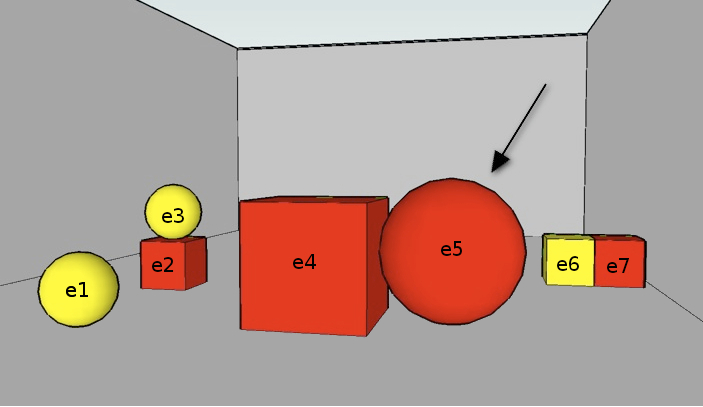
\includegraphics[width=\textwidth]{images/22.jpg}
%\vspace*{1cm}
%\caption{Input scene}
\label{GRE3D7-stimulus-22}
\end{subfigure}
%\hspace*{-0.35cm}
\begin{subfigure}{.5\textwidth}
  \centering
%\includegrahics[width=\textwidth]{images/22sinletras.jpg}
%%\caption{Ejemplo de contexto}
%\label{GRE3D7-stimulus1-b}
%\vspace*{1cm}
\begin{picture}(250,0)
\put(0,-80){\begin{tikzpicture}
  [
    n/.style={circle,draw,inner sep=1.5pt,node distance=1.5cm},
		 aArrow/.style={->, >=stealth, semithick, shorten <= 1pt, shorten >= 1pt},
  ]
 \node[n,label=below:{
    \relsize{-2}$\begin{array}{c}
		  \nLeft\\[-3pt]
      \nSmall\\[-3pt] 
      \nYellow \\[-3pt] 
      \nBall\end{array}$}] (a) {$e_1$};
 \node[n,label=below:{
    \relsize{-2}$\begin{array}{c} 
		  \nLeft\\[-3pt]
      \nSmall\\[-3pt] 
      \nRed\\[-3pt] 
      \nCube\end{array}$}, right of=a] (b) {$e_2$};
 \node[n,label=above:{
    \relsize{-2}$\begin{array}{c}
      \nTop\\[-3pt]
      \nLeft\\[-3pt]
      \nSmall\\[-3pt] 
      \nYellow\\[-3pt] 
      \nBall\end{array}$}, above of=b] (c) {$e_3$};
 \node[n,label=below:{
    \relsize{-2}$\begin{array}{c}
      \nLarge\\[-3pt] 
      \nRed\\[-3pt] 
      \nCube\end{array}$}, right of=b] (d) {$e_4$};
 \node[n,label=below:{
    \relsize{-2}$\begin{array}{c}
      \nLarge\\[-3pt] 
      \nRed\\[-3pt] 
      \nBall\end{array}$}, right of=d] (e) {$e_5$};
 \node[n,label=below:{
    \relsize{-2}$\begin{array}{c}
      \nSmall\\[-3pt] 
      \nYellow\\[-3pt] 
      \nCube\end{array}$}, right of=e] (f) {$e_6$};
 \node[n,label=below:{
    \relsize{-2}$\begin{array}{c}
      \nSmall\\[-3pt]
      \nRed\\[-3pt] 
      \nCube\end{array}$},  right of=f] (g) {$e_7$};
 \draw [aArrow,bend right=40] (b) to node[auto,swap]{\relsize{-3}$\nBelow$} (c);
 \draw [aArrow,bend right=40] (c) to node[auto,swap]{\relsize{-3}$\nOntop$} (b);
 \draw [aArrow,bend right=40] (d) to node[auto,swap]{\relsize{-3}$\nLeftof$} (e);
 \draw [aArrow,bend right=40] (e) to node[auto,swap]{\relsize{-3}$\nRightof$} (d);
 \draw [aArrow,bend right=40] (f) to node[auto,swap]{\relsize{-3}$\nLeftof$} (g);
 \draw [aArrow,bend right=40] (g) to node[auto,swap]{\relsize{-3}$\nRightof$} (f);
 %\draw[dotted] (-0.5,-1.3) rectangle (8,3.1);
 \draw[dotted] (-0.5,-1.8) rectangle (8,3.7);
 \end{tikzpicture}}
 \end{picture}
%\end{flushleft}
\end{subfigure}
\caption{Contexto y modelo del ejemplo de ejecuci\'on.}\label{fig4-9}
\end{figure}

La primer relaci\'on a considerar de acuerdo a las R.\puse\ es \texttt{ball}, recordemos que la relaci\'on \texttt{ball} se a\~nadir\'a a $RE$ si su interpretaci\'on 
tiene al menos un elemento, $\interp{\top \cup \texttt{ball}}$\footnote{Como las relaciones unarias se transformaron en binarias, la f\'ormula que el algoritmo agregar\'a sera $\top \cup \exists\ .\texttt{ball}~\top$. Aqu\'i escribimos $\top \cup \texttt{ball}$ por simplicidad.} no tiene que ser vac\'io, y su interpretaci\'on tiene que ser distinta de $\interp{\top}$. Ambas condiciones se cumplen y $RE$ entonces es \{$\top$, \texttt{ball}\}. Se ven los elementos de la f\'ormula \texttt{ball} en el recuadro de la Figura~\ref{fig-modelo3} que enmarca a $e_1$, $e_3$ y $e_5$.

\begin{figure}[ht]
\begin{center}
\frame{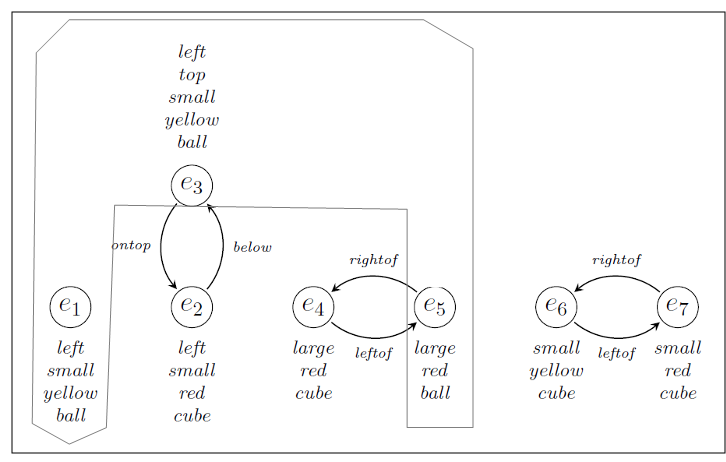
\includegraphics[width=8cm]{images/ej/1ball.png}}\\[0pt]
\caption{Elementos que satisfacen la f\'ormula \texttt{ball}.}
\label{fig-modelo3}
\end{center}
\end{figure}

La siguiente propiedad a considerar es \texttt{cube}. Realizando el mismo procedimiento antes mencionado, queda $\interp{\texttt{ball}}$ = $\{e_1,e_3,e_5\}$ y
$\interp{\texttt{cube}}$ = $\{e_2, e_4, e_6, e_7\}$. $RE$ =\{$\top$, \texttt{ball}, \texttt{cube}\}. Notar que las particiones de  \texttt{ball} y \texttt{cube} hacen que $\top$ no agregue informaci\'on es decir $\top$ est\'a subsumida, por lo tanto podemos borrarla. Quedando las particiones como se muestra en la Figura~\ref{fig-modelo4}.

%\setlength{\unitlength}{1cm}
%
%\newsavebox{\mybox} 
%\savebox{\mybox}{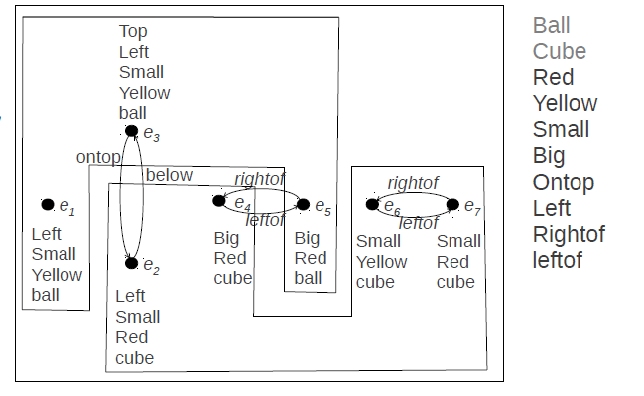
\includegraphics[scale=0.40]{images/modelo4.png}} 
 %\begin{figure}
   %\begin{picture}(8,6)
  %\put(0,0){\usebox{\mybox}} 
  %%\put(2,2.5){\oval(6,5)}
   %\end{picture}   
 %\end{figure} 

\begin{figure}[ht]
\begin{center}
\frame{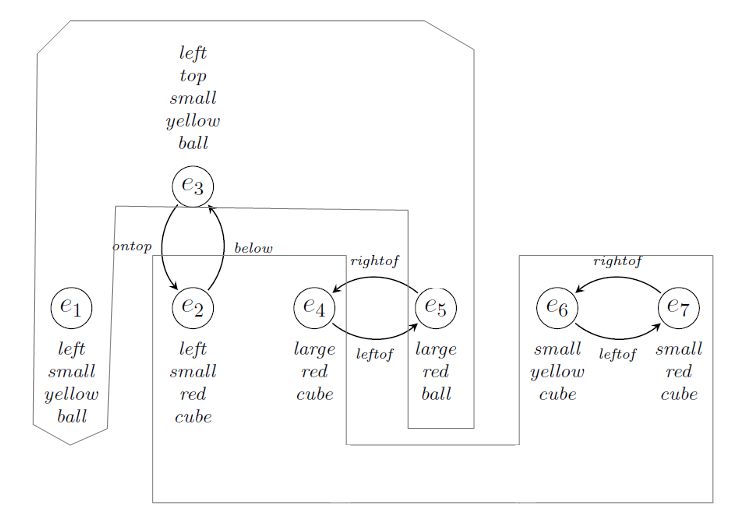
\includegraphics[width=8cm]{images/ej/2ball-cube.png}}\\[0pt]
\caption{Cuadros indicando \texttt{ball} y \texttt{cube}.}
\label{fig-modelo4}
\end{center}
\end{figure}
La siguiente propiedad es \texttt{red}, donde  
$\interp{\texttt{red}}$ = $\{e_2, e_4, e_5, e_7\}$, haciendo la intersecci\'on con la $\interp{.}$ de cada f\'ormula en $RE$ obtenemos, 
$\{e_5\}$ y $\{e_2, e_4, e_7\}$. Las particiones actuales se pueden ver en la Figura~\ref{fig-modelo9}. El conjunto $RE$ hasta el momento es $\{\texttt{ball}, \texttt{cube}, \texttt{ball} \wedge \texttt{red}, \texttt{cube} \wedge \texttt{red}\}$.

\begin{figure}[ht]
\begin{center}
\frame{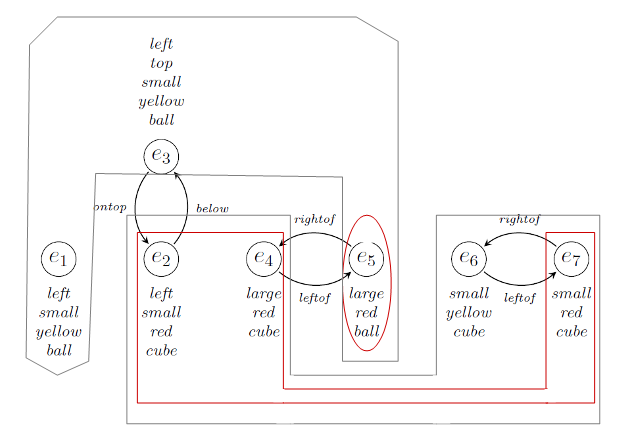
\includegraphics[width=8cm]{images/ej/3ball-cube-red.png}}\\[0pt]
\caption{Cuadros indicando \texttt{ball}, \texttt{cube} y \texttt{red}.}
\label{fig-modelo9}
\end{center}
\end{figure}
%
Siguiendo con \texttt{yellow}, tenemos que $\interp{\texttt{yellow}}$ = $\{e_1, e_3, e_6\}$ y obtenemos $RE$ = $\{\texttt{ball} \wedge \texttt{yellow}, 
\texttt{cube} \wedge \texttt{yellow}, \texttt{ball} \wedge \texttt{red}, \texttt{cube} \wedge \texttt{red}\}$. 
Note que aqu\'i ya borramos la f\'ormula \texttt{ball} porque estaba subsumida, y la f\'ormula \texttt{cube} tambi\'en. Se muestran las particiones resultantes en Figura~\ref{fig-modelo10}.

\begin{figure}[ht]
\begin{center}
\frame{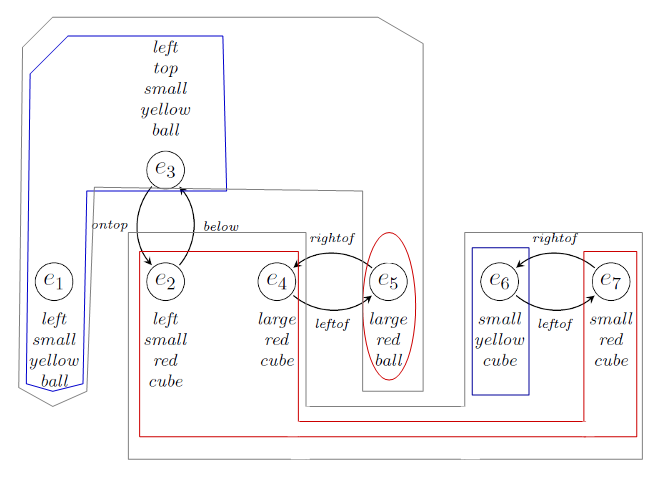
\includegraphics[width=8cm]{images/ej/4ball-cube-red-yellow.png}}\\[0pt]
\caption{Cuadros indicando \texttt{ball}, \texttt{cube}, \texttt{red} y \texttt{yellow}.}
\label{fig-modelo10}
\end{center}
\end{figure}

Borrando subsumidas del modelo tenemos
\begin{figure}[ht]
\begin{center}
\frame{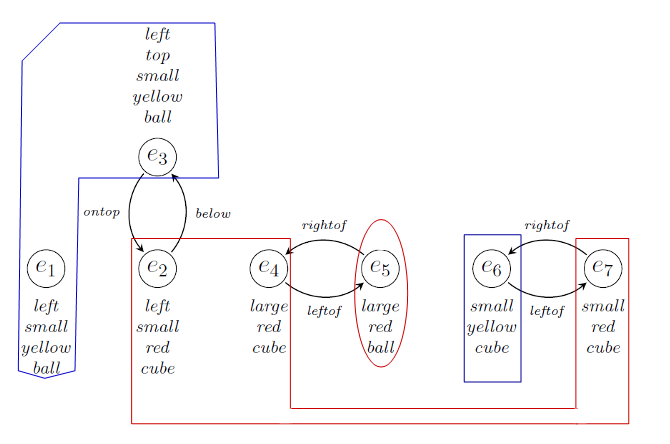
\includegraphics[width=8cm]{images/ej/4b.png}}\\[0pt]
\caption{Cuadros indicando \texttt{ball}, \texttt{cube}, \texttt{red} y \texttt{yellow}, sin subsumidas.}
\label{fig-modelo10}
\end{center}
\end{figure}

Haciendo lo mismo con \texttt{small} tenemos $RE$ = $\{\texttt{ball} \wedge \texttt{yellow} \wedge \texttt{small}, \texttt{cube} \wedge \texttt{yellow} \wedge \texttt{small}, \texttt{ball} \wedge \texttt{red}, \texttt{cube} \wedge \texttt{red}, \texttt{cube} \wedge \texttt{red} \wedge \texttt{small}\}$, las particiones resultantes se pueden ver en Figura~\ref{fig-modelo11}.

%\setlength{\unitlength}{1cm}
%
%\newsavebox{\mybox} 
%\savebox{\mybox}{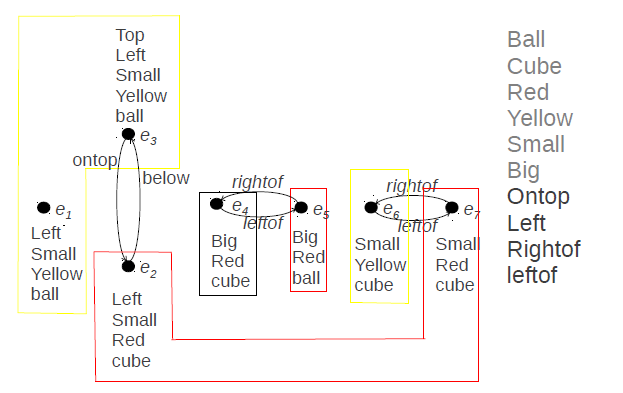
\includegraphics[scale=0.40]{images/modelo11.png}} 
 %\begin{figure}
   %\begin{picture}(8,6)
  %\put(0,0){\usebox{\mybox}} 
  %%\put(2,2.5){\oval(6,5)}
   %\end{picture}   
 %\end{figure} 

\begin{figure}[ht]
\begin{center}
\frame{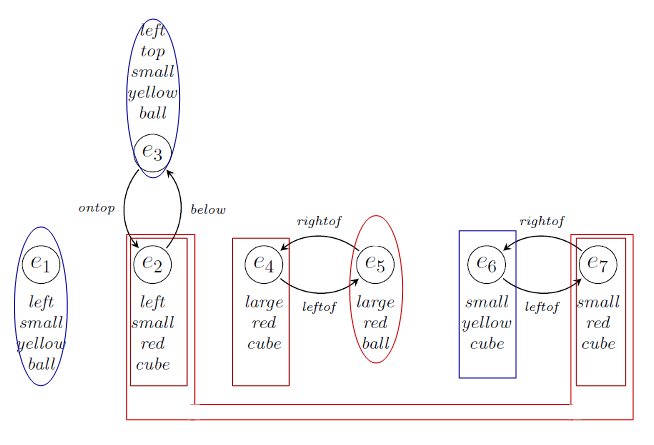
\includegraphics[width=8cm]{images/ej/5ball-cube-red-yellow-large-small.png}}\\[0pt]
\caption{Cuadros indicando \texttt{ball}, \texttt{cube}, \texttt{red}, \texttt{yellow}, \texttt{small} y \texttt{large}.}
\label{fig-modelo11}
\end{center}
\end{figure}

La siguiente propiedad es \texttt{large} as\'i, tenemos $RE$ = $\{\texttt{ball} \wedge \texttt{yellow} \wedge \texttt{small}, \texttt{cube} \wedge \texttt{yellow} \wedge \texttt{small}, \texttt{ball} \wedge \texttt{red}, \texttt{cube} \wedge \texttt{red} \wedge \texttt{large}, \texttt{cube} \wedge \texttt{red} \wedge \texttt{small}\}$. Aqu\'i no podemos agregar \texttt{large} a la f\'ormula $\texttt{red} \wedge \texttt{cube}$ porque su interpretaci\'on tiene un s\'olo elemento, y la condici\'on dice que es necesario tener m\'as de uno (y no estamos en el primer ciclo).

Hasta ahora $RE$ = $\{\texttt{ball} \wedge \texttt{yellow} \wedge \texttt{small}, \texttt{cube} \wedge \texttt{yellow} \wedge \texttt{small}, \texttt{ball} \wedge \texttt{red}, \texttt{cube} \wedge \texttt{red} \wedge \texttt{large}, \texttt{cube} \wedge \texttt{red} \wedge \texttt{small}\}$ 
y tenemos las siguientes extensiones: $\{e_1, e_3\}, \{e_6\}, \{e_5\}, \{e_4\}, \{e_2, e_7\}$ respectivamente. 
Hay dos f\'ormulas que a\'un pueden ser refinadas, $\texttt{ball} \wedge \texttt{yellow} \wedge \texttt{small}$ y $\texttt{cube} \wedge \texttt{red} \wedge \texttt{small}$ 
debido a que tienen m\'as de un elemento cada una, por lo que entran en el ciclo, while del Algoritmo \ref{algo:bisim-l}. Ahora es el turno de las relaciones, la primera de ellas es \texttt{leftof}, para cada f\'ormula $\varphi$ en $RE$ trataremos de hacer add$_\el$ (\texttt{leftof},$\varphi$, $RE$). Notar que $\psi$ solo puede ser $\texttt{ball} \wedge \texttt{yellow} \wedge \texttt{small}$ o $\texttt{cube} \wedge \texttt{red} \wedge \texttt{small}$ porque estas tienen en su interpretaci\'on m\'as de un elemento. 


\begin{figure}[ht]
\begin{center}
\frame{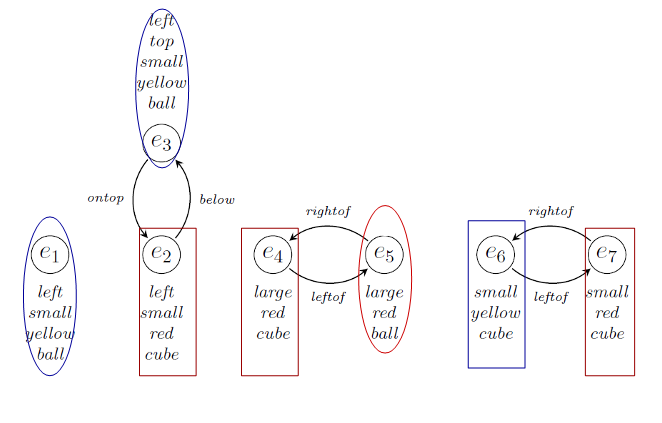
\includegraphics[width=8cm]{images/ej/5b.png}}\\[0pt]
\caption{Cuadros indicando ``ball'', ``cube'', ``red'', ``yellow''...}
\label{fig-modelo15}
\end{center}
\end{figure}


No hay
%because those are the ones that its interpretation have more than one element. There is not 
$\varphi$ y $\psi$ que puedan ser aplicadas. Continuando con \texttt{rightof} agregamos $\texttt{cube} \wedge \texttt{yellow} \wedge \texttt{small} \wedge \exists \texttt{rightof}. \texttt{cube} \wedge \texttt{red} \wedge \texttt{small}$, y as\'i con \texttt{ontop} agregamos $\texttt{small} \wedge \texttt{red} \wedge \texttt{cube} \wedge \exists \texttt{ontop}. \texttt{small} \wedge \texttt{yellow} \wedge \texttt{ball}$ y el algoritmo termina con ER = $\{\texttt{ball} \wedge \texttt{yellow} \wedge \texttt{small}, \texttt{cube} \wedge \texttt{yellow} \wedge \texttt{small}, \texttt{ball} \wedge \texttt{red}, \texttt{cube} \wedge \texttt{red} \wedge \texttt{large}, \texttt{cube} \wedge \texttt{red} \wedge \texttt{small}, \texttt{cube} \wedge \texttt{yellow} \wedge \texttt{small} \wedge \exists \texttt{rightof}. \texttt{cube} \wedge \texttt{red} \wedge \texttt{small}, \texttt{small} \wedge \texttt{red} \wedge \texttt{cube} \wedge \exists \texttt{ontop}. \texttt{small} \wedge \texttt{yellow} \wedge \texttt{ball}\}$, 
aqu\'i todos los elementos est\'an en una clase singleton y no se puede hacer ning\'un refinamiento m\'as. 
%can be applied to $cubo \wedge red \wedge peque\~no$ but there is no formula which interpretation has more than one element to be apply with this one. The same happen for the other relations, so the algorithm ends.
%its interpretation is $\{e_7\}$ with $\psi$ is $cubo \wedge yellow \wedge peque\~no$, the others combinations can't be apply because they don't do true the preconditions. The following relation is rightof, 

%leftof, rightof, ontopof, bellowof

%At this point we already have the target in a singleton set. So the formula for it is ``red and esfera'', and also for s6 which formula is ``yellow cubo''.\\
%As we show this algorithm depends of the order of properties and relations.\\



\begin{figure}[ht]
\begin{center}
\frame{\includegraphics[width=8cm]{images/modelo16.png}}\\[0pt]
\caption{Cuadros indicando ``ball'', ``cube'', ``red'', ``yellow''...}
\label{fig-modelo16}
\end{center}
\end{figure}

\begin{figure}[ht]
\begin{center}
\frame{\includegraphics[width=8cm]{images/modelo17.png}}\\[0pt]
\caption{Cuadros indicando ``ball'', ``cube'', ``red'', ``yellow''...}
\label{fig-modelo17}
\end{center}
\end{figure}

Las expresiones referenciales de salida dadas por el algoritmo son:
\begin{itemize}
\item $\texttt{ball} \wedge \texttt{yellow} \wedge \texttt{small}$ representa $e_1$, la cual se puede realizar como \textit{La esfera amarilla peque\~na} 
\item $\texttt{small} \wedge \texttt{red} \wedge \texttt{cube} \wedge \exists \texttt{ontop}. \texttt{small} \wedge \texttt{yellow} \wedge \texttt{ball}$ representa $e_2$, la cual se puede realizar como \textit{El cubo peque\~no y rojo que est\'a arriba de la peque\~na bola amarilla}.
\item $\texttt{cube} \wedge \texttt{red} \wedge \texttt{large}$ representa $e_4$, la cual se puede realizar como \textit{El cubo rojo y grande} 
\item $\texttt{ball} \wedge \texttt{red}$ representa $e_5$, la cual se puede realizar como \textit{La esfera roja} 
\item $\texttt{cube} \wedge \texttt{yellow} \wedge \texttt{small}$ representa $e_6$, que puede realizarse como \textit{El peque\~no cubo amarillo} 
\item $\texttt{cube} \wedge \texttt{red} \wedge \texttt{small}$ representa $\{e_2,e_7\}$, la cual se puede realizar como \textit{Los cubos rojos peque\~nos}  
\item $\texttt{cube} \wedge \texttt{yellow} \wedge \texttt{small} \wedge \exists \texttt{rightof}. \texttt{cube} \wedge \texttt{red} \wedge \texttt{small}$ representa $e_6$, la cual se puede realizar como \textit{El peque\~no cubo amarillo que est\'a a la derecha del peque\~no cubo rojo} 
 
\end{itemize}


\subsection{Asegurando terminaci\'on}

Uno de los problemas que ten\'ian otros algoritmos es que no siempre terminaban, para asegurar terminaci\'on nosotros incrementamos las probabilidades aleatorias en cada ciclo, hasta que alcancen 1. Definimos MaxIterations como la cantidad m\'axima de iteraciones que vamos a permitir, y calculamos R.incuse es cuanto vamos a incrementar la probabilidad de R en cada ciclo, R.incuse = (1 -R.puse) / MaxIterations, con esto nos aseguramos que en MaxIterations todas lleguen a 1, y en consecuencia el algoritmo termine, ya que en el c\'odigo, se incrementa R.puse con R.incuse y sale del ciclo principal si para todas las R, R.puse son mayores o iguales a 1.
Este es un algoritmo de punto fijo, se refinan las particiones hasta que en alg\'un momento no se pueden hacer m\'as refinamientos, se dice que el algoritmo llego a un punto fijo, en el que no le es posible progresar $RE$ se mantiene sin modificaciones. Las particiones se van haciendo m\'as chicas en las sucesivas iteraciones y considerando que la cantidad de elementos del modelo y las relaciones son finitas, el algoritmo siempre termina.

\subsection{Generando ER relacionales}

Nuestro algoritmo permite generar relaciones con otros objetos e incluir expresiones de los dem\'as objetos (no necesariamente ERs), no tiene preferencia por las relaciones ni por las propiedades proposicionales (como otros algoritmos descriptos de trabajo previo), en el sentido de que va o no incluirlas de acuerdo a la probabilidad de uso que ellas tengan, las cuales fueron calculadas o aprendidas de un corpus.

\subsection{Generando ER no-determin\'isticamente}

Al iniciar el algoritmo calcula para cada R, R.\randomuse que es un n\'umero aleatorio entre 0 y 1, ese n\'umero va a hacer que el algoritmo sea no-determin\'istico, ya que, el algoritmo usar\'a R para refinar las clases solamente si 
R.rnduse >= R.puse. Por lo tanto y considerando que en las siguientes ejecuciones R.rnduse ser\'an distintos, va a poder generar distintas ER.

\subsection{Generando descripciones sobreespecificadas}\label{sec:overspecification}

El algoritmo hace caso omiso de la restricci\'on de informatividad (es decir, que permite la inclusi\'on de nuevas relaciones
en la descripci\'on, incluso si no refinan la clase asociada) \emph{pero s\'olo durante el
primer ciclo del algoritmo}. Es decir, durante el primer ciclo sobre los elementos de la
lista de probabilidades Rs, se permitir\'a la inclusi\'on de todas las relaciones que no trivializan la
descripci\'on (es decir, la clase asociada no est\'a vac\'{i}a). Debido a que esto se hace s\'olo durante
el primer ciclo, sabemos que no aparecer\'an propiedades repetidas en las ERs generadas (como \texttt{green green ball}).
En los ciclos restantes, se a\~nadir\'an propiedades adicionales s\'olo si son de car\'acter informativo.
Este dise\~no del algoritmo que permite sobreespecificaci\'on est\'a inspirado en la obra de \cite{keysar:Curr98} sobre el egocentrismo y la producci\'on del lenguaje natural. Keysar et al. argumentan que cuando se produce el lenguaje, el hablante no identifica un\'ivocamente al target desde el principio, sino que  
es m\'as bien un ajuste de \'ultimo momento. Los hablantes producen ERs primero egoc\'entricamente, agregando aquellas propiedades m\'as prominentes por m\'as de que no sean informativas. Pero luego las ajustan de modo que el destinatario de la ER sea capaz de identificarla. El primer paso, egoc\'entrico, es un proceso
heur\'istico basado en un modelo de la prominencia de la propiedades de la escena que contiene el target. Nuestra definici\'on de
\puse\ est\'a destinada a capturar las prominencias de las propiedades de diferentes escenas y targets. Los valores de \puse\
cambian en relaci\'on a la escena considerada. Esto est\'a en contraste con el trabajo previo donde
la prominencia de una propiedad es constante en un dominio. Keysar et al. argumentan que la raz\'on del procedimiento de 
generar-y-ajustar puede tener que ver con las limitaciones de procesamiento de informaci\'on de la
mente: si la heur\'istica que gu\'ia la fase egoc\'entrica est\'a bien sintonizada, consigue una adecuada ER al principio
y rara vez requerir\'a ajustes. Se observa un comportamiento similar
con nuestro algoritmo: cuando los valores de \puse\ son
aprendidos del dominio, el algoritmo no es
s\'olo es m\'as preciso, sino que tambi\'en es mucho m\'as r\'apido que cuando se utilizan valores de \puse\ aleatorios. Por ejemplo la ER \texttt{large red ball} generada por el algoritmo para el target $e_5$ de la Figura \ref{}, las primeras palabras dichas son \texttt{large red} que son las propiedades m\'as sobresaliente del objeto target. 


%\subsection{Generando ER para plurales}
%
%Este algoritmo devuelve ER para todos los elementos del contexto, 
%esto implica que podr\'iamos dar expressiones referenciales de un conjunto de elementos.
%
%Por ejemplo queremos identificar a $e_1$ y $e_5$ 
%siendo resultados dados por el algoritmo que $e_1$
%ball, yellow, small
%y $e_5$ ball, red
%

\section{Notas finales y linkeo del cap\'itulo}
\label{sec:link-algoritmo}

En este cap\'itulo se explic\'o la entrada y salida de un algoritmo probabil\'istico. Una de las entradas es el modelo, el cual es una representaci\'on de la figura considerada. Otra es una distribuci\'on de probabilidades finita, la cual explicamos como obtenerla en 2 casos. Primero en el caso que hay corpus disponible para la escena considerada y en casos donde al no haber corpus disponible proponemos una aproximaci\'on usando aprendizaje autom\'atico. Se explic\'o el algoritmo en detalle y se ilustr\'o con un ejemplo de ejecuci\'on. Se explic\'o c\'omo hace el algoritmo para conseguir las siguientes caracter\'isticas: asegurar terminaci\'on, generar ER relacionales, generar ER no-determin\'isticas y generar sobreespecificaci\'on.
El dise\~no del algoritmo est\'a inspirado en el modelo cognitivo de generaci\'on de expresiones referenciales de \cite{keysar:Curr98}. En el Cap\'itulo \ref{sec:evaluacion} veremos que este algoritmo es capaz de generar rankings de ERs cercanos a los encontrados en corpora.
El algoritmo presentado en este cap\'itulo introduce una familia de algoritmos que extiende probabil\'isticamente a los algoritmos presentados en el Cap\'itulo \ref{sec:intro_logica}. Se explicaron los detalles de la subrutina \textit{add} para el lenguaje \EL. Las definiciones de \textit{add} para otros lenguajes como \ALC o \EPFOL son similares.
Como se discuti\'o en el Cap\'itulo \ref{sec:intro}, los dominios realistas de posibles aplicaciones de la GER contienen incertidumbre. En este cap\'itulo modelamos esa incertidumbre como las probabilidades de usar una caracter\'istica en una ER. 
Estos algoritmos pueden tambi\'en ser usados con probabilidades provenientes de confidence scores de sensores, por ejemplo, para modelar otros tipos de incertidumbre.
En el Cap\'itulo \ref{sec:evaluacion} evaluamos estos algoritmos sobre un corpus de descripciones de mapas, el corpus ZOOM.
% generar ER para plurales.
%
%En el c\'alculo de probabilidades de uso de las palabras con nuestra versi\'on simplista, podemos ver cosas interesantes como por ejemplo que {\it ball} tiene una \puse\ alta, ya que en el corpus considerado todos los targets son {\it ball}, en cambio la probabilidad de {\it cube} no es tan alta y depende de la discernibilidad, si aparece, aparece en la descripci\'on del landmark. Para {\it blue} y {\it green} el valor de \puse\ depende de si el target es {\it blue} o {\it green}, entonces si el target es {\it blue}, le d\'a un valor alto a {\it blue} y bajo a {\it green} y viceversa. Las relaciones {\it ontop}, {\it leftof} y {\it rightof} dependen fuertemente si el target tiene o no esa relaci\'on y en caso de tenerla igualmente la \puse\ no es muy alta, esto indica que en un porcentaje del 30\% por ejemplo se usa {\it ontop} y en menos del 3\% {\it leftof} o {\it rightof}, ya reportado en trabajo previo. Vimos que el tama\~no es m\'as frecuente usado para sobreespecificaci\'on cuando el target y el landmark tienen el mismo tama\~no (es usado en ERs sobreespecificadas el 49\% cuando el target y el landmark comparten el tama\~no, y s\'olo el 25\% cuando no lo comparten).
%Hay algunas relaciones complejas entre las caracter\'{i}sticas de las escenas que no somos capaces de
%capturar. La caracter\'{i}stica m\'as importante del dominio \textit{GRE3D7}
%que no somos capaces de aprender, y tiene un impacto en nuestro desempe\~no, es que
%las propiedades de tama\~no (es decir, small y large) se utilizan mucho
%m\'as cuando el target no puede ser identificado s\'olo con las propiedades taxon\'omicas absolutas 
%(verde y azul) y (ball y cube). En otras palabras, en el corpus \textit{GRE3D7} se utiliza el tama\~no con m\'as frecuencia (90,2 \%)
%cuando la ER resultante no es sobreespecificada y cuando si es sobreespecificada el (34 \%). \\


\chapter{Probabilidades de uso}
\label{sec:learning}


%\subsection{Aprendizaje autom\'atico desde un corpus para describir nuevos objetos}

En el cap\'itulo anterior hemos presentado un algoritmo que supone que para
cada relaci\'on R se tiene una conocida probabilidad de uso R.\puse. En esta secci\'on, se dan algunas posibilidades de c\'omo
calcular estas probabilidades de uso.

Por otro lado, al ser nuestro algoritmo no-determinista en 2 ejecuciones podr\'ia dar diferentes ER para el mismo target y conjunto de probabilidades de uso, incluso si estas son aleatorias.

Luego en el Cap\'itulo \ref{sec:evaluacion} 

\section{Aleatoriamente}

Una posibilidad es dar a cada relaci\'on de la signatura del modelo, una probabilidad de uso aleatoria, es facil de calcular, y dado que el algoritmo asegura dar una expresi\'on referencial si existe, calcular las probabilidades de uso en forma aleatoria ser\'ia una posibilidad.


\section{Uniformemente}

Lo malo de poner esto aca, es que la forma en que lo evaluamos despues no fue exactamente asi, fue uniforme en las er no en las prob de uso... pensar si dejo esto...

\section{A partir de corpus}

Supongamos que tenemos disponible un corpus de ER asociada a diferentes escenas t\'{i}picas del dominio en el que el algoritmo GER tiene que operar. 


\subsection{Calculando \puse\ cuando hay disponible un corpus para la escena considerada}

Las Figuras \ref{rojo-amarillo} y  \ref{verde-azul} son las escenas del corpus GRE3D7 introducido en \ref{sec:corpusGRE}, est\'an agrupadas seg\'un los colores que tienen.\\

\begin{figure}
\centering
\includegraphics[width=1\textwidth]{images/rojo-amarillo.png}
\caption{Im\'agenes del GRE3D7 parte rojo y amarillo}
\label{rojo-amarillo}
\end{figure}

\begin{figure}
\centering
\includegraphics[width=1\textwidth]{images/imagenesML.png}
\caption{Im\'agenes del GRE3D7 parte azul y verde}
\label{verde-azul}
\end{figure}


\begin{figure}[ht]
\begin{minipage}[b]{0.5\linewidth}
\centering
\includegraphics[width=\textwidth]{images/3.jpg}
%\vspace*{1cm}
\caption{Contexto 3 del GRE3D7}
\label{fig3}
\end{minipage}
\hspace*{1cm}
\begin{minipage}[b]{0.5\linewidth}
%\centering
%\begin{figure}[ht]
%\begin{center}
green ball \\
small green ball  \\
small green ball on-top red large cube \\
green ball on-top blue cube\\
green ball on-top large blue cube \\
small green ball on-top blue cube  \\
ball on-top cube \\
small green ball on-top red large left cube  \\
small ball on-top cube large  \\
top green ball   \\
green ball on-top cube  \\
\caption{ER dadas por personas para el Contexto \ref{fig3}}
\label{ER-fig3}
\end{minipage}
\end{figure}


El corpus tiene para cada imagen 140 ER dadas por personas. Las ER dadas en \ref{ER-fig3} son las ER diferentes que aparecieron en el corpus para el Contexto \ref{fig3}, pero... uno se imagina un corpus en que las personas usaron distintas palabras para nombrar lo mismo, distintas frases, distinto orden de las palabras, s\'i es verdad, este corpus ya est\'a limpio de todas esas cosas, pero si quisieramos partir de un corpus con las ER tal cual dieron las personas, tendr\'iamos que realizar los siguientes pasos a fin de unificar el vocabulario:

\begin{enumerate}
\item Tokenizar las expresiones referenciales y llamar al conjunto de palabras distintas
 $Pal$. En particular, las expresiones de varias palabras como ``arriba de'', ``encima de''
  debe ser igualadas a una \'unica palabra que signifique lo mismo, digamos \emph{arriba-de}.

\item Eliminar hiper\'onimos de $Pal$. Por ejemplo, si ambos \emph{cubo} y
  \emph{cosa} aparecen en $Pal$ para nombrar la misma cosa, eliminar \emph{cosa}, ya que \emph{cubo} es m\'as espec\'ifico.

\item Si el conjunto de palabras obtenidas en los pasos anteriores contiene
  sin\'onimos normalizarlos con un representante de la clase.  Por ejemplo, las palabras \emph{chico}
  y \emph{peque\~no} son ambas representadas por la palabra \emph{peque\~no}.

\item Llamar al conjunto resultante $\REL$; que ser\'a la signatura del modelo $\gM$ utilizada por el algoritmo.

\item Para cada escena, definir $\gM$ tal que la interpretaci\'on
 $\interp {\cdot}$ asegure de que todas las ERs encontradas en el corpus sean ER en
  el modelo. Por ejemplo, las %$\el$ f\'ormulas correspondientes%
	ER de \ref{ER-fig3} deben denotar el target se\~nalado en la Figura \ref{fig3} el modelo 
$\gM$ est\'a representado en Figura~\ref{modelo-fig3}.
%GRE3D7-stimulus-cap2
\item Para cada R$\in \REL$ calculo R.\puse \ utilizando~(\ref{eq1}) si
  hay muchas ER para cada escena (caso corpus GRE3D7) o asignamos 1 a R.\puse \ si R esta en ER, asignamos 0 en caso contrario (caso corpus TUNA).
\end{enumerate}

En el caso del GRE3D7 ya estaba unificado el vocabulario y la signatura del modelo es 
$\REL = \{green, ball, small, ontop, red, large, cube, blue, left, top\} $

\begin{figure}[ht]
\centering
\begin{tikzpicture}
  [
    n/.style={circle,fill,draw,inner sep=3pt,node distance=2cm},
    aArrow/.style={->, >=stealth, semithick, shorten <= 1pt, shorten >= 1pt},
  ]
 \node[n,label=above:$e_1$,label=below:{
    \relsize{-1}$\begin{array}{c}
      \nLeft\\[-2pt]
      \nSmall\\[-2pt] 
      \nBlue\\[-2pt]
      \nBall\end{array}$}] (a) {};

 \node[n,label=above:$e_2$,label=below:{
    \relsize{-1}$\begin{array}{c}
      \nLeft\\[-2pt]
      \nBig\\[-2pt] 
      \nBlue\\[-2pt]
      \nCube\end{array}$}, right of=a] (b) {};

 \node[n,label=below:$e_3$,label=above:{
    \relsize{-1}$\begin{array}{c}
      \nTop\\[-2pt]      
			\nLeft\\[-2pt]
      \nSmall\\[-2pt]      
			\nGreen\\[-2pt]
      \nBall\end{array}$}, above of=b] (c) {};

 \node[n,label=above:$e_4$,label=below:{
    \relsize{-1}$\begin{array}{c}
      \nSmall\\[-2pt] 
      \nGreen\\[-2pt] 
      \nCube\end{array}$}, right of=b] (d) {};

 \node[n,label=above:$e_5$,label=below:{
    \relsize{-1}$\begin{array}{c}
      \nBig\\[-2pt] 
      \nBlue\\[-2pt] 
      \nBall\end{array}$}, right of=d] (e) {};

 \node[n,label=above:$e_6$,label=below:{
    \relsize{-1}$\begin{array}{c}
      \nBig\\[-2pt] 
      \nGreen\\[-2pt] 
      \nCube\end{array}$}, right of=e] (f) {};

 \node[n,label=below:$e_7$,label=above:{
    \relsize{-1}$\begin{array}{c}
      \nTop\\[-2pt]
      \nSmall\\[-2pt]
      \nBlue\\[-2pt]
      \nCube\end{array}$}, above of=f] (g) {};

 \draw [aArrow,bend right=90] (b) to node[auto,swap]{\relsize{-1}$\nBelow$} (c);
 \draw [aArrow,bend right=90] (c) to node[auto,swap]{\relsize{-1}$\nOntop$} (b);

 \draw [aArrow,bend right=30] (d) to node[auto,swap]{\relsize{-1}$\nLeftof$} (e);
 \draw [aArrow,bend right=30] (e) to node[auto,swap]{\relsize{-1}$\nRightof$} (d);

 \draw [aArrow,bend right=90] (f) to node[auto,swap]{\relsize{-1}$\nBelow$} (g);
 \draw [aArrow,bend right=90] (g) to node[auto,swap]{\relsize{-1}$\nOntop$} (f);
\draw[dotted] (-0.5,-1.4) rectangle (9.7,3.7);
 %\draw[dotted] (-.65,-1.2) rectangle (7.1,2.1);

 \end{tikzpicture}
\vspace*{-.4cm}\caption{El modelo del Contexto \ref{fig3}}
\label{modelo-fig3}
\end{figure}

La regresi\'on lineal es un m\'etodo matem\'atico que modela la relaci\'on que hay entre una variable dependiente Y, las variables independientes Xi y un t\'ermino aleatorio E.  \\

Vamos a tomar la parte \ref{verde-azul} del corpus GRE3D7 para aprender las probabilidades de uso de cada palabra en las ER que di\'o la gente, y as\'i darnos una idea de como es la distribuci\'on del uso de las palabras del conjunto $REL$ en el corpus.\\

Vamos a usar las siguientes propiedades, las cuales las sacamos autom\'aticamente del XML del corpus.

\begin{small}
\begin{table}[h]
\begin{center}
\begin{tabular}{|l|p{10cm}|}
\hline
target-tiene & cuando el elemento target tiene la propiedad. \\
\#rel-prop & n\'umero de propiedades y relaciones que el target tiene.\\
\#rel & n\'umero de relaciones que el target tiene. \\
landmark-tiene & cuando un landmark del target tiene la propiedad, un objeto es un landmark si tiene una relaci\'on directa en el modelo, con el target (lo usamos para el GRE3D7).\\
location-has & cuando la RE puede usar la ubicaci\'on del target en la figura (esto se hizo porque el TUNA corpus tiene algunas ER donde se le dijo a la gente que pod\'ian usar la localizaci\'on del objeto).\\
discrimination & calculada como 1 sobre el n\'umero de objetos en el modelo que tienen la propiedad.  \\
\hline
\end{tabular}
\caption{Caracter\'isticas usadas para conseguir f\'ormulas con regresi\'on lineal que nos den una idea de la \puse\ de las palabras} 
\label{features}
\end{center}
\end{table}
\end{small}

\begin{table}[h!]
\begin{center}
\caption{F\'ormulas y errores de regresi\'on lineal para todo el corpus \ref{verde-azul}}
\label{tabla-linear-regresion-all}
\begin{tabular}{|l|c|c|l|}
\hline
Palabra &Error promedio	LR	& Error-PM	& F\'ormula de LR\\
\hline
ball		 &0.0465   &0.0609	  & 0.2894 * disc-gatt + 0.7883\\
\hline
cube		 &0.0417	 &0.0531	  &0.49   * disc-gatt - 0.0129\\
\hline
\hline
blue		 &0.0353	 &0.0454	  &0.848  * target-tiene + 0.1073\\
\hline
green		 &0.0264	 &0.046	    &0.8722 * target-tiene + 0.0016\\
\hline
\hline
large		 &0.1762	 &0.2378	  &0.5911 * target-tiene + 0.0354\\
\hline
small		 &0.1499	 &0.1755	  &0.3918 * target-tiene + 0.2478 * landmark-tiene -\\
				 &				 &					&0.0913\\
\hline
\hline
left-of  &0.0041	 &0.0094	  &0.0131 * target-tiene +\\
				 &				 &					&0.0253 * adj-target-tiene - 0.0507\\
\hline
on-top	 &0.0706	 &0.1594	  &0.2942 * target-tiene \\
\hline
right-of &0.0029	 &0.0049	  &0.0153 * target-tiene + 0.001\\
\hline
\hline
left		 &0.0068	 &0.0101	  &0.0346 * adj-target-tiene - 0.0653\\
\hline
right		 &0.0079	 &0.0092	  &-0.0118 * disc-gatt + 0.0141\\
\hline
front    &0.0099 	 &0.0135		& 0.0069\\
\hline
center	 &0.0023	 &0.0037	  &0.0047 * target-tiene + 0.0047 * adj-target-tiene +\\
				 &				 &					&0.0029 * vecino-tiene - 0.009\\
\hline
\end{tabular}
\end{center}
\end{table}

En la Tabla \ref{tabla-linear-regresion-all} podemos ver por ejemplo que {\it ball} tiene una \puse\ alta, es natural ya que en el corpus \ref{verde-azul} todos los targets son {\it ball}, en cambio se puede ver que {\it cube} no es tan alta y depende de la discernibilidad, este n\'umero en la \puse\ debe leerse como la probabilidad de usar {\it cube} en la descripci\'on del landmark. En los casos de {\it blue} y {\it green} el valor de \puse\ depende de si el target es {\it blue} o {\it green}, entonces si el target es {\it blue}, le da un valor alto a {\it blue} y bajo a {\it green} y viceversa, no depende del valor de discernibilidad en el modelo.
En la tabla tambi\'en podemos ver que relaciones como {\it small} y {\it large} tienen un error mucho mas alto que el resto de las relaciones, esto se debe a que ellas son propiedades vagas... 
Las relaciones {\it ontop}, {\it leftof} y {\it rightof} dependen fuertemente si el target tiene esa relaci\'on y en caso de tenerla igualmente la \puse\ no es muy alta, esto indica que en un porcentaje del 30\% por ejemplo se usa {\it ontop} y en menos del 3\% {\it leftof} o {\it rightof}, esta observaci\'on fue reportada en (Viethen, 2011)
Una caracter\'istica interesante que se no fue mencionada en trabajo previo es que tama\~no es m\'as frecuente usado para sobreespecificaci\'on cuando el target y el landmark tienen el mismo tama\~no 
(es usado en ER sobreespecificadas el 49\% cuando el target y el landmarck comparten el tama\~no, y s\'olo el 25\% cuando no lo comparten)


Supongamos que queremos generar autom\'aticamente ER para el target $t$ en una
determinada escena, y que tenemos disponible un corpus $C$ de ER de $t$
en esa escena (esto es exactamente el tipo de informaci\'on que encontramos en el
GRE3D7 corpus \textit{y en el TUNA-corpus}). Utilizamos las ER de $C$
para definir el modelo relacional utilizado por el algoritmo. Entonces 
estimaremos el valor de \puse\ para cada una de las relaciones en el modelo como el
porcentaje en que aparece la relaci\'on en las ER. Es decir,
\begin{equation} \label{eq1}
R.\puse = \frac {\#\mbox{de ERs en $C$ en el que aparece R}} {\#\mbox{de las ER en $C$}}.
\end{equation}

En el caso del corpus TUNA el c\'alculo no es necesario
porque tenemos solo una ER para cada escena.

Esta estimaci\'on es demasiado simplificada y, por ejemplo, no 
diferencia las propiedades del target y las propiedades de
los landmarks utilizadas en una ER relacional para completar la descripci\'on
del target. Pero es muy f\'acil de calcular, y vamos a ver
en la Secci\'on~\ref{sec:evaluacion} que ya produce ER naturales
que coinciden con las encontradas en el corpus.


Las ERs, cantidad de ocurrencias y porcentaje del corpus para de la Figura~\ref{GRE3D7-stimulus-cap2} se muestran en la tabla~\ref{corpus-distribution}, la signatura resultante y su asociado \puse\ figuran en las tres primeras columnas de la tabla~\ref{probability-of-use}.\\

ARREGLAR ESTA TABLA HABIA UNO MAL... ver original...
\begin{table}[h!]
\begin{center}
\begin{tabular}{|l|c|c|}
\hline
Expresiones Referenciales & Cantidad de ocurrencias & Porcentage \\
\hline

green ball & 91 & 65.00\% \\
small green ball   & 23 & 16.43\% \\
small green ball on-top red large cube & 8 & 5.71\% \\
green ball on-top blue cube & 5 & 3.57\% \\
green ball on-top large blue cube & 5 & 3.57\% \\
small green ball on-top blue cube & 2 & 1.43\% \\
ball on-top cube & 1 & 0.71\% \\
small green ball on-top red large left cube  & 1 & 0.71\% \\
small ball on-top large cube & 1 & 0.71\% \\
top green ball  & 1 & 0.71\% \\
%peque\~no esfera on-top cube small & 1 & 0.71\% \\
green ball on-top cube & 1 & 0.71\% \\

\hline
\end{tabular}
\caption{Expresiones Referenciales producidas por las personas para la Figura~\ref{GRE3D7-stimulus-cap2}}\label{corpus-distribution}
\end{center}
\end{table}


Observe que los valores R.\puse\ obtenidos de esta manera deben ser
interpretados como la probabilidad de utilizar R para describir el target en
modelo de $\gM $, y podr\'{i}amos argumentar que se correlacionan con la
 prominencia de R en el modelo. Por esa raz\'on, por ejemplo, el
valor de \emph{esfera}.\puse\ es 1, mientras que el valor de
\emph{cubo}.\puse\ es 0.178. \\

Estas probabilidades no ser\'an \'utiles
para describir los diferentes targets en diferentes escenas. Veremos c\'omo se
pueden utilizarlas para obtener valores para los nuevos targets y escenas utilizando un
enfoque de aprendizaje autom\'atico en la siguiente secci\'on. No es de extra\~nar,
que usando estos valores para R.\puse\ las ER generadas con mayor frecuencia por el
algoritmo se puedan encontrar en el corpus. Como discutiremos en la Secci\'on~\ref{sec:evaluacion} el algoritmo genera ER
con una distribuci\'on que coincide con la encontrada en el corpus y, como la
Tabla~\ref{results-algo-fig3} muestra, incluso las ER generadas por el algoritmo que no se encontraron
en el corpus son naturales.


\subsection{Calculando \puse\ para el target para escenas sin corpus } 
\label{subsec:learning}

%If there is no corpora that describes the target we can estimate the
%\puse~from corpora on a different scenes in the same domain.
%
%We use simple features to obtain the function, all the features can be
%extracted automatically from the relational model and are listed in

Si no hay corpus de expresiones referenciales que describen el target, se puede estimar la \puse~a partir de corpus de
diferentes escenas en el mismo dominio.
Usamos caracter\'isticas simples para obtener una funci\'on que nos dar\'a la probabilidad de cada palabra en el nuevo modelo, todas las caracter\'isticas se pueden extraer de forma autom\'atica desde el modelo relacional y se enumeran en la Tabla~\ref{features}.

\begin{small}
\begin{table}[h]
\begin{center}
\begin{tabular}{|l|p{10cm}|}
\hline
target & cuando el elemento target tiene la propiedad. \\
\#rel-prop & n\'umero de propiedades y relaciones que el target tiene.\\
\#rel & n\'umero de relaciones que el target tiene. \\
landmark & cuando un landmark del target tiene la propiedad, un objeto es un landmark si tiene una relaci\'on directa en el modelo, con el target (lo usamos para el GRE3D7).\\
location-has & cuando la RE puede usar la ubicaci\'on del target en la figura (esto se hizo porque el TUNA corpus tiene algunas ER donde se le dijo a la gente que pod\'ian usar la localizaci\'on del objeto).\\
discrimination & calculada como 1 sobre el n\'umero de objetos en el modelo que tienen la propiedad.  \\
\hline
\end{tabular}
\caption{Caracter\'isticas usadas para aprendizaje autom\'atico de las \puse~para cada palabra en la signatura de los modelos de \textit{GRE3D7 y TUNA-corpus} \label{features}}
\end{center}
\end{table}
\end{small}

En el caso del GRE3D7 usamos la parte verde-azul, es decir todas las im\'agenes que tienen colores verde y azul, para acotar el problema, asumiendo que la otra parte dar\'ia algo similar. En la siguiente figura se muestran los contextos considerados.


Para hacer el aprendizaje, separamos 1 contexto al que llamamos testing, y todos los dem\'as de entrenamiento. Por ejemplo para aprender \puse\ del contexto 13, se usaron los contextos: 1,3,6,8,10,12,15,18,20,21,23,25,27,30 y 32. Y as\'i sucesivamente para los dem\'as contextos.

Nuestro conjunto de caracter\'{i}sticas es intencionadamente simplista con el fin de que sea
independiente de dominio. Como resultado hay algunas relaciones complejas
entre las caracter\'{i}sticas de las escenas que no es capaz de
capturar. La caracter\'{i}stica m\'as importante del dominio GRE3D7
que no somos capaces de aprender, y tiene un impacto en nuestro desempe\~no, es que
las propiedades de tama\~no (es decir, peque\~no y grande) se utilizan mucho
m\'as cuando el target no puede ser identificado s\'olo con las propiedades taxon\'omicas absolutas 
(verde y azul) y (esfera y cubo). En otras palabras, en el corpus GRE3D7 se utiliza el tama\~no con m\'as frecuencia (90,2 \%)
cuando la ER resultante no es sobreespecificada y cuando si es sobreespecificada el (34 \%). 
Puede que no sea posible aprender esta caracter\'{i}stica de los
datos del GRE3D7 ya que incluso con las funciones que dependen de dominio definidos
en~\cite[Cap\'{i}tulo 6] {viet:gene11}, no pod\'{i}a ser aprendido por \'arboles decisi\'on. 
Como resultado podemos ver en la tabla~\ref{probability-of-use} de la Figura 13, el valor estimado para 
``grande'' no est\'a cerca de la
valor calculado a partir de corpus. \textit{En el caso de la TUNA-corpus
  mostramos que no podemos aprender la dependencia de la dimensi\'on-X y
  dimensi\'on-y, es decir, cuando una persona a\~nade dimensi\'on-x es altamente
  probable que incluya la dimensi\'on-y en su expresi\'on referencial.}


\begin{figure}[ht]
\begin{minipage}[b]{0.5\linewidth}
\centering
\includegraphics[width=\textwidth]{images/3.jpg}
%\vspace*{1cm}
\caption{Escena 3 del GRE3D7}
\label{GRE3D7-stimulus-3}
\end{minipage}
%\hspace*{-0.35cm}
\begin{minipage}[b]{0.5\linewidth}
\centering
%\begin{figure}[ht]
%\begin{center}
\includegraphics[width=\textwidth]{images/13.jpg}
\caption{Escena 13 del GRE3D7}
\label{GRE3D7-stimulus-13}
\end{minipage}
\end{figure}

\begin{table}[h!]
\begin{center}
\begin{tabular}{|l|c|c|c|c|}
\hline
Palabra &  \puse 					& \puse\ Aprendida & \puse\    							& \puse\  Aprendida \\
        & Modelo \ref{GRE3D7-stimulus-3}   & \ref{GRE3D7-stimulus-3} 				& Modelo \ref{GRE3D7-stimulus-13} 			&  \ref{GRE3D7-stimulus-13}  \\
\hline
esfera & 1.0 & 1.0 & 1.0 & 1.0 \\
cubo & 1.0 & 1.0 & 1.0 & 1.0 \\
verde & 0.978 & 0.993 & 1.0 & 0.9875 \\
peque\~no & 0.257 & 0.346 & 0.0428 & 0.1993 \\
arriba-de & 0.178 & 0.179 & 0 & 0\\ 
azul & 0.15 & 0.124 & 0.064 & 0.1353 \\
grande & 0.107 & 0.03 & 0.307 & 0.7378 \\
izquierda & 0.007 & 0.002 & 0 & 0.0024 \\
arriba & 0.007 & 0 & 0 & 0 \\
derecha & 0 & 0.001 & 0.064 & 0.0005 \\
a-la-izq-de & 0 & 0 & 0 & 0 \\
a-la-der-de & 0 & 0 & 0.064 & 0.1023 \\
debajo-de & 0 & 0 & 0 & 0 \\
\hline
\end{tabular}
\caption{Probabilidades de uso de las palabras del corpus \textit{(GRE3D7) para las Figuras\ref{GRE3D7-stimulus-3} y \ref{GRE3D7-stimulus-13} } 
\label{probability-of-use}}
\end{center}
\end{table}

El aprendizaje se realiza con el kit de herramientas de aprendizaje autom\'atico
WEKA~\cite{Hall:WEK09}, entrenando con todas las escenas menos una (para la que estamos aprendiendo) para todas las escenas del \textit{GRE3D7 y TUNA-corpus}. \\
Ejemplo de xml \ref{archivos-xml-tuna}. Notar que no teniamos las imagenes, armamos algunas necesarias nomas, pero no sabemos la unicaci\'on exacta de los objetos.\\

Un ejemplo de archivo de los que toma WEKA como input es para la propiedad blue de la parte muebles del corpus TUNA es \ref{archivos-arff-blue}. 
No recuerdo si esto lo usamos al final o no...
\ref{probabilidad-GATT} , \ref{algoritmo-GATT} 

Utilizamos regresi\'on lineal para aprender la funci\'on de
\puse\ para cada palabra en la signatura. Para una escena determinada, reemplazamos
las variables de la funci\'on obtenida por los valores de las caracter\'{i}sticas
de la escena que queremos describir.\\

Con regresi\'on lineal podemos aprender caracter\'{i}sticas interesantes
 del dominio. Para empezar, se aprenden hechos conocidos
como que color aparezca en la ER depende en gran medida de si el
target es de ese color, y que no depende de su
poder de discriminaci\'on en el modelo. Por otra parte, vimos que la relaci\'on arriba-de
 se utiliza con m\'as frecuencia que las relaciones horizontales
(izquierda y derecha) lo que confirma un hallazgo previo informado
en~\cite{viet:gene11}. Por \'ultimo, vimos en el
GRE3D7 corpus (que no fue reportado por el trabajo anterior), se utiliza el tama\~no
m\'as frecuentemente de una manera sobreespecificada cuando el
target y el landmark comparten el tama\~no. El tama\~no fue utilizado en ER de manera sobreespecificada en el 49 \% de
las descripciones de escenas en las que el target y el landmark compart\'ian el tama\~no,
y el 25 \% cuando target y el landmark no lo compart\'ian. Esto puede explicarse por la observaci\'on de que si landmark y el target comparten una propiedad, esta propiedad es m\'as relevante.



\chapter{Evaluaci\'on de rankings sobre benchmarks}
\label{sec:evaluacion}

En esta secci\'on se presentan diversas formas de evaluar a los algoritmos propuestos en el cap\'itulo anterior. En particular, se muestra que el algoritmo de refinamiento probabil\'{i}stico con sobreespecificaci\'on es capaz de generar un ranking de ERs que es similar a la distribuci\'on de frecuencias de las ERs observadas en corpora usando m\'etricas autom\'aticas y que tambi\'en tiene un buen desempe\ ~no cuando se usan m\'etricas manuales. 

%Este cap\'itulo esta dividido en tres secciones, en la primera secci\'on se muestra un ejemplo de ranking de ERs del corpus GRE3D7 comparado con el ranking de ERs generadas por el algoritmo de refinamiento probabil\'istico, usando probabilidades de uso aprendidas desde las dem\'as im\'agenes del GRE3D7. Se comparan ambos rankings y se d\'a la presici\'on, es %decir el porcentaje de matcheo perfecto. Se muestran las ERs generadas por el algoritmo que no estan en el corpus, y se argumenta que son buenas para identificar al target igual que las dem\'as. Luego en la Secci\'on \ref{sec:compara-varias} explicamos la misma comparaci\'on pero teniendo en cuenta todas las escenas verde-azules del corpus GRE3D7 y hacemos comparaciones de rankings de ERs dadas por nuestro algoritmos con 3 diferentes distribuciones de probabilidades como entrada, contra las ERs humanas existentes en el corpus. Mostramos la entrop\'ia cruzada entre las distribuciones propuestas y la del corpus. El corpus usado para la comparaci\'on es el GRE3D7 ya que ese corpus tiene un ranking de ERs dadas por humanos para cada escena.
%, Incluso cuando no se dispone de corpus espec\'{i}fica para un objeto de destino determinado.

%Se discuten en detalle los experimentos ejecutados para la escena que se muestra en la Figura~\ref{GRE3D7-stimulus},  %(escena 3 en el corpus GRE3D7)
%a continuaci\'on, un resumen de los resultados de las otras siete escenas que utilizamos para las pruebas.
%https://docs.google.com/spreadsheets/d/1Hn2fqQZBqkJscUE62UakNsKmMKOvLodvLoAbztT6kV4/edit#gid=6 en drive

\section{Evaluaci\'on de rankings sobre el corpus GRE3D7}
\label{sec:compara}
En esta sección presentamos una evaluación cuantitativa y automática de los algoritmos en el dominio del corpus GRE3D7~\cite{gre3d7} introducido en la Seccion~\ref{sec:corpusGRE} del Capítulo~\ref{sec:seleccion}. Mostraremos una comparaci\'on con el ranking de ERs dadas por el algoritmo con las probabilidades de uso calculadas como se describe en la Secci\'on~\ref{sec:learning}, es decir con aprendizaje autom\'atico a partir de las dem\'as im\'agenes del corpus y ejecutando nuestro algoritmo 10000 veces. El algoritmo probabilístico con sobreespecificación es capaz de generar una distribución de ERs similar a la que se observa en el corpus. Describimos primero en detalle los experimentos que realizamos para la escena que se muestra en la Figura~\ref{contexto-evaluacion}, en la Sección \ref{sec:compara}. Luego, en la Sección \ref{sec:compara-varias}, resumimos los resultados obtenidos en evaluaciones similares para otras 7 escenas del corpus. 
\subsection{Caso de estudio de una escena del corpus GRE3D7}

Las probabilidades de uso aprendidas usando regresión lineal como se muestra en el Capítulo~\ref{sec:learning} se muestran en \ref{probabilidades-escena2}, y ejecutando el algoritmo 10000 veces.

\begin{table}[H]
\begin{center}
\footnotesize{
\begin{tabular} {  l c c c c c c c c c c}
\hline
%\multicolumn{1}{c}{}
%&\multicolumn{1}{c}{Domain}
%&\multicolumn{3}{c}{Descriptions}\\

R				&{\it ball}			& {\it cube}	& {\it green}	  & {\it blue} & {\it large} & {\it small} & {\it top} & {\it front} & {\it left} & {\it ontop}   \\
\hline
R.\puse	& 1.0			& 1.0		& & &  &   &  & & & \\
\hline

\end{tabular}
}
\end{center}
\vspace*{-.5cm} 
\caption{Distribuci\'on de probabilidad de las propiedades y relaciones de la figura de ejemplo.}\label{probabilidades-escena2}

Obtuvimos 14 expresiones referenciales diferentes para la escena de la Figura~\ref{contexto-evaluacion}, el corpus tiene 12 ERs diferentes generadas por personas para esa escena. Es interesante ver que aunque es posible generar cientos de ERs para esta escena, el algoritmo, guíado por las probabilidades de uso, genera sólo 14 ERs en 10000 ejecuciones. Además, el algoritmo genera, para esta imagen, 2 ERs con alta frecuencia (la bola verde y la bola verde pequeña representan el 98% de las ERs generadas automáticamente) y otras ERs con una frecuencia mucho menor (representan el 2% de las ERs generadas). Estas 2 ERs más frecuentes generadas por el algoritmo coincide con las 2 ERs más frecuentes generadas por las personas (la bola verde y la bola verde pequeña representan el 81% de las ERs generadas por humanos para la imagen). 
 
\begin{figure}[!ht]
\centering
\includegraphics[width=.6\textwidth]{images/3.jpg}\\[0pt]
\label{fig-GRE3D7}
\caption{Imagen del GRE3D7 corpus.}\label{contexto-evaluacion}
\end{figure}

La \textbf{precisi\'on}  es una m\'etrica autom\'atica estricta que se puede usar para comparar rankings de ERS. Es la proporci\'on de coincidencias perfectas entre la salida de algoritmo y las ERs generadas por humanos y encontradas en corpora. 
La primer comparaci\'on de rankings de ERs se muestra en la Tabla \ref{results-algo-fig3}. Para cada ER, indicamos el n\'umero de veces que aparece en el corpus (\#Cor), la proporci\'on que representa (\%Cor), el n\'umero de veces que la gener\'o nuestro algoritmo (\#Alg) y la proporci\'on que representa (\%Alg).
Por \'ultimo, la precisi\'on (\%Acc) nos d\'a el porcentaje de aciertos de las ERs generadas por el algoritmo y se calcula como el m\'inimo entre el \%Cor y \%Alg. 

\begin{table}[H]
\begin{small}
\begin{center}
\begin{tabular}{|l|r|r|r|r|r|}
\hline
\multirow{2}{*}{Expresiones Referenciales} & \multicolumn{2}{|c|}{Corpus} & \multicolumn{2}{|c|}{Algoritmo} & Precisi\'on \\ \cline{2-6} 
 & \#Cor & \multicolumn{1}{|c|}{\%Cor} & \multicolumn{1}{|c|}{\#Alg} & \multicolumn{1}{|c|}{\%Alg} & \multicolumn{1}{|c|}{\%Acc} \\
\hline
ball, green                                    & 91 & 65.00 & 6376 & 63.76 & 63.76 \\
ball, green, small                              & 23 & 16.43 & 3440 & 34.40 & 16.43 \\
ball, green, small, ontop(blue, cube, large)      &  8 &  5.71 &    0 &  0.00 &  0.00\\
ball, green, ontop(blue, cube)                  &  5 &  3.57 &    0 &  0.00 &  0.00\\
ball, green, ontop(blue, cube, large)            &  5 &  3.57 &    0 &  0.00 &  0.00\\
ball, green, small, ontop(blue, cube)            &  2 &  1.43 &    0 &  0.00 &  0.00\\
ball, ontop(cube)                             &  1 &  0.71 &   27 &  0.27 &  0.27 \\
ball, green, small, ontop(blue, cube, large, left) &  1 &  0.71 &    0 &  0.00 &  0.00\\
ball, small, ontop(cube,large)	              &  1 &  0.71 &    2 &  0.02 &  0.02 \\
ball, green, top                                &  1 &  0.71 &    0 &  0.00 &  0.00\\
ball, small, ontop(cube)                       &  1 &  0.71 &    3 &  0.03 &  0.03 \\
ball, green, ontop(cube)                       &  1 &  0.71 &    0 &  0.00 &  0.00\\
ball, front, green                              &  0 &  0.00 &   97 &  0.97 &  0.00\\
ball, front, green, small                        &  0 &  0.00 &   13 &  0.13 &  0.00\\
ball, front, top                                &  0 &  0.00 &   12 &  0.12 &  0.00\\
ball, green, left	                              &  0 &  0.00 &   11 &  0.11 &  0.00\\
ball, top                                      &  0 &  0.00 &   10 &  0.10 &  0.00\\
ball, green, left, small                         &  0 &  0.00 &    5 &  0.05 &  0.00\\
ball, left, top                                 &  0 &  0.00 &    2 &  0.02 &  0.00\\
ball, small, top                                &  0 &  0.00 &    1 &  0.01 &  0.00\\
ball, front, ontop(cube, left)                  &  0 &  0.00 &    1 &  0.01 &  0.00\\

\hline
Total & 140 & 100 & 10000 & 100 & 80.51 \\
\hline
\end{tabular}
\caption{ERs del corpus, y las producidas por nuestro algoritmo para la Figura~\ref{contexto-evaluacion}.\label{results-algo-fig3}}
\vspace*{-.5cm}
\end{center}
\end{small}
\end{table}

 La precisi\'on del algoritmo con respecto al corpus GRE3D7 para esta escena es del 80\%. De las 14 ERs diferentes generadas por el algoritmo, 5 se encuentran en el corpus y las otras 9 no. Estas 9 expresiones referenciales incluyen propiedades de ubicación del target no con respecto a un landmark si no a su posición en la escena 3D. Por ejemplo \emph{la espera verde que está a la izquierda} se refiere a que la esfera verde está a la izquierda de la escena.  La probabilidad de uso de este tipo de propiedades es menor al 1 \%, en particular la de left es 0,007, pero, como esa probabilidad no es cero, dichas propiedades aparecen en ERs (siempre con menos de un 1% de frecuencia).  La m\'etrica de precisi\'on ha sido utilizada en trabajos anteriores para comparar la salida de un algoritmo de generaci\'on de ER con las ERs que se encuentran en corpora~\cite{sluis07:eval,viet:gene11} y se considera una m\'etrica muy estricta para esta tarea.

\subsection{Evaluaci\'on emp\'irica sobre el resto del corpus}
\label{sec:compara-varias}

Como es habitual cuando hacemos una evaluaci\'on con un caso particular, podemos pensar, que como el algoritmo tiene un componente de azar, por eso nos di\'o bastante bien, para esa ejecuci\'on particular. Por eso aqu\'i se muestra la misma comparaci\'on realizada en la secci\'on anterior pero con todas las im\'agenes verde-azules del corpus GRE3D7. 
Para enriquecer esta parte mostraremos otros baselines, los cuales dos dar\'an pistas de que las probabilidades de uso aprendidas con el m\'etodo que presentamos en esta tesis son \'utiles para aproximar al ranking de ERs que aparece en corpora. Los baselines que se presentan ejecutan el algoritmo con una distribuci\'on aleatoria de probabilidades de uso, y con una distribuci\'on uniforme (en las ERs tomando tanto las generadas por el sistema como las del corpus y las generadas como el modelo aleatorio). El Top baseline, es en el que el algoritmo us\'o las probabilidades de uso sacadas del corpus mismo. 

\begin{table}[h!]
\begin{small}
\begin{center}
\begin{tabular}{|l|c|c|c|c|}
\hline
         &  \puse\ de escena & \puse\ aprendidas & \puse\ random & uniforme \\ \hline
Escena 1	&	85.75\%	&	84.49\%	&	17.95\%	&	5.37\%	\\
Escena 3	&	82.81\%	&	80.51\%	&	9.89\%	&	4.40\%	\\
Escena 6	&	90.11\%	&	83.30\%	&	4.13\%	&	4.16\%	\\
Escena 8	&	86.52\%	&	64.06\%	&	16.32\%	&	9.75\%	\\
Escena 10	&	89.49\%	&	75.80\%	&	7.56\%	&	3.70\%	\\
Escena 12	&	80.21\%	&	81.29\%	&	57.09\%	&	6.68\%	\\
Escena 13	&	89.98\%	&	50.79\%	&	9.30\%	&	3.59\%	\\
Escena 21	&	92.13\%	&	80.01\%	&	8.45\%	&	6.77\%	\\
\hline
Promedio	&	87.13\%	&	75.03\%	&	16.34\%	&	5.55\%	\\

\hline
\end{tabular}
\caption{Precisi\'on entre las ERs del corpus y las generadas usando valores de \puse\ calculados desde la escena, aprendidos autom\'aticamente, provenientes de distribuciones random y uniformes.}\label{results-algo-all}
\end{center}
\end{small}
\end{table}


La primera columna muestra los valores obtenidos cuando corremos el algoritmo sobre la escena
con los valores de \puse\ obtenidos~\emph{de la propia escena}. Como se puede esperar,
esta columna tiene el mayor promedio de precisi\'on.

La segunda columna muestra los resultados del algoritmo cuando se ejecuta con \puse\ aprendido de
corpora como se explica en la Secci\'on~\ref{sec:learning} del cap\'itulo anterior. Este es el caso m\'as interesante porque muestra la capacidad de nuestra propuesta de generalizar a escenas no vistas con anterioridad y para las que no hay corpus. Para la mayor\'{i}a de las escenas la precisi\'on
es mayor al 80\% y la precisi\'on promedio es 75\%. La relativamente baja precisi\'on
obtenida en la escena 13 se explica principalmente las pobres estimaciones del valor de~\puse\ para las palabras \emph{large} y \emph{small} que son propiedades vagas y no absolutas ya que dependen de cu\'an grandes son en relaci\'on con los otros elementos del contexto.  

En el corpus, las relaciones \emph{large} y \emph{small} se utilizan mucho m\'as cuando el target no puede ser identificado usando s\'olo propiedades taxon\'omicas (\emph{ball} y \emph{cube}) y propiedades absolutas (\emph{green} y \emph{blue}), pero las caracter\'{i}sticas que hemos utilizado para el aprendizaje autom\'atico no capturan dichas dependencias como se discute en la Secci\'on \ref{sec:learning-corpus} del Cap\'itulo \ref{sec:algoritmo}.

A pesar de esta limitaci\'on, el promedio de la segunda columna es 75\%. Para una m\'etrica como la de precisi\'on que es considerada demasiado estricta, estos resultados son buenos. Adem\'as, el 25\% no cubierto por el algoritmo puede contener ERs igualmente buenas como evaluamos en la Secci\'on \ref{sec:humanevaluation}. Uno podr\'ia argumentar entonces que los valores de \puse\ aprendidos a partir del corpus son lo suficientemente buenos para ser utilizados para generar REs para nuevas escenas del dominio.

Las dos \'ultimas columnas pueden ser consideradas como baselines. En la primera generamos
valores aleatorios para \puse\. La precisi\'on obtenida es en la mayor\'{i}a de los casos pobre, pero con
una variaci\'on notable debido al azar. Adem\'as estas ejecuciones toman mucho m\'as tiempo en finalizar, lo que indica que se est\'an realizando demasiadas particiones sin conseguir llegar a la meta. Esta observaci\'on de performance es consistente con los resultados de los experimentos de generaci\'on humana realizados por \cite{keysar:Curr98,} y discutidos en la Seccion \ref{sec:psicolinguistica} del Cap\'itulo \refsec:seleccion}. Keysar argumenta que, las personas usan la prominencia de las propiedades en el dominio como heur\'istica para guiar la generaci\'on de ERs de forma de disminuir la carga cognitiva de tener que probar con todas las propiedades del dominio. Si la heur\'istica es buena, en muchos casos no es necesario ``revisar'' la ER para que identifique un\'ivocamente al target. Como efecto colateral de este proceso heur\'istico la ER resultante puede estar sobreespecificada, pero se genera r\'apidamente.  

Adem\'as de poca precisi\'on, cuando se utilizaron probabilidades random,  muchas de las ERs generadas suenan poco natural y son dif\'iciles de realizar sin introducir ambig\"uedades como, por ejemplo, (\textit{peque\~na cosa sobre
el cubo azul que est\'a abajo de algo que es peque\~no}). En la \'ultima columna se presenta la precisi\'on de una corrida artificial, le llamamos uniforme, uniforme tomando todas las ERs de las dem\'as columnas y asign\'andoles la misma probabilidad.
Para comparar nuestros resultados colos 3 baselines usamos tambi\'en entrop\'ia cruzada.
En teor\'ia de la informaci\'on, la \textbf{entrop\'ia cruzada} entre dos distribuciones de probabilidad mide la media de bits necesarios para identificar un evento de un conjunto de posibilidades, si un esquema de codificaci\'on est\'a basado en una distribuci\'on de probabilidad dada q, m\'as que en la verdadera distribuci\'on p. Vamos a comparar la entrop\'ia cruzada entre la distribuci\'on de probabilidad que se encuentra en el corpus, y la distribuci\'on de ER del corpus y las de ejecuciones del algoritmo con las probabilidades que acabamos de describir~(ver~\cite{juraksky:spee08} para obtener detalles sobre evaluaci\'on de entrop\'{i}a cruzada). En la Figura~\ref{Entropy} se muestran los resultados para las ocho escenas que hemos considerado.

\begin{figure}[ht]
\centering
\includegraphics[width=0.6\textwidth]{images/entropy.jpg}
\caption{Entrop\'ia cruzada entre la distribuci\'on del corpus y diferentes ejecuciones del algoritmo.}\label{Entropy}
\end{figure}
  
Las entrop\'{i}as cruzadas de las dos primeras ejecuciones (\emph{escena} y \emph{aprendizaje autom\'atico}) son, en general, mucho m\'as cercanas de la entrop\'{i}a del corpus, que las entrop\'ias cruzadas de \emph{random} y \emph{uniforme}. S\'olo en la escena 12 random, por azar se acerca un poco m\'as.

%En esta secci\'on presentamos dos evaluaciones diferentes que realizamos en nuestro algoritmo. Secci\'on~\ref{sec:automaticevaluation} describe una evaluaci\'on con respecto al estado del arte~\cite{KrahmerGRAPH}. GRAPH fue el de mejor desempe\~no en las dos ediciones de la competencia ASGRE~\cite{gatt-balz-kow:2008:ENLG}. Debido a las limitaciones de los indicadores autom\'aticos, en la Secci\'on~\ref{sec:humanevaluation} realizamos una evaluaci\'on humana en la que pedimos a jueces humanos comparar la salida producida por nuestro algoritmo con las expresiones producidas por los seres humanos (las del corpus).


\section{Evaluaci\'on de rankings en el TUNA Challenge} \label{sec:automaticevaluation}

En esta secci\'on se presenta la comparaci\'on de nuestro algoritmo con el algoritmo que tuvo el mejor desempe\~no en el TUNA Challenge. 

\subsection{El TUNA Challenge}
El TUNA Challenge ...

El algoritmo GRAPH que describimos en el Cap\'itulo \ref{sec:seleccion} es un algoritmo determin\'stico y por lo tanto produce la misma expresi\'on referencial cuando se ejecuta con el mismo target y contexto. Nuestro algoritmo es no-determin\'istico, puede dar una expresi\'on referencial diferente cada vez que se ejecuta. Con el fin de compararlos corremos nuestro algoritmo 100 veces y hacemos un ranking de las 20 ERs ordenadas por la frecuencia que se produjeron. Utilizamos la parte de prueba del corpus TUNA (el cual fue introducido en la Secci\'on \ref{sec:corpusTUNA}), para comparar el ranking de ERs dado por nuestro algoritmo con las salidas del algoritmo GRAPH cuyos resultados se describen en~\cite{KrahmerGRAPH} y se reproducen en la Tabla~\ref{Tabla_sis_1_20}.


\subsection{Comparaci\'on con el TUNA Challenge}
El algoritmo GRAPH define la generaci\'on de expresiones referenciales como un problema de b\'usqueda en un grafo, devuelve el grafo distintivo de menor costo (si existe) dada una funci\'on de costo particular. Comparamos a este algoritmo usando las m\'etricas precisi\'on, Dice y \textsc {masi}, introducidas en la Secci\'on \ref{sec:metricasAutomaticas}. 

Recordemos que el corpus TUNA tiene 2 partes, una parte cuyo dominio son muebles, y otra parte cuyo dominio son personas, ambos ubicados en una grilla. Para realizar esta comparaci\'on se us\'o s\'olamenta la parte singular del corpus.

En la Tabla~\ref{Tabla_sis_1_20} mostramos m\'etricas autom\'aticas y comparamos la performance de nuestro sistema con el sistma GRAPH para la primer ER en el ranking y para las primeras 20 ERs del ranking.

\begin{table}[H]
\begin{center}
\begin{tabular}{|l|c|c|c|}
\hline
%Figure & Model \puse &  Learning \puse & Random \puse &  Uniform \puse \\
	 	& 	Dice		&	\textsc{masi}	&	Precisi\'on		\\
\hline
sistema GRAPH, Dominio muebles	& 	80\% 		&	59\%	&	48\%		 	\\
sistema GRAPH, Dominio personas 	& 	72\%		&	48\%	&	28\%			\\
\hline
Nuestro sistema, Dominio muebles (top 1)	&	80\%		&	60\%	&	47\%		\\
Nuestro sistema, Dominio personas (top 1)	&	65\%		&	37\%	&	19\%		\\
\hline
Nuestro sistema, Dominio muebles (top 20)&	87\%		&	75\%  	&	65\%		\\
Nuestro sistema, Dominio personas (top 20)   &	81\%		&68\%	&	60\%		\\
\hline
\end{tabular}
%\vspace*{.1cm}
\caption{Comparaci\'on del algoritmo GRAPH y nuestro sistema. Consideramos 3 m\'etricas autom\'aticas para el top 1 y para el top 20 ERs producidas por nuestro algoritmo.}
%\vspace*{-.5cm}
\label{Tabla_sis_1_20}
\end{center}
\end{table}
%\vspace*{-.5cm}
%Accuracy, Dice and \textsc{masi} assess humanlikeness with respect to a corpus of human referring expressions. In the Figure~\ref{graficoPresicion} the accuracy for our system and the GRAPH system is compared. The left GRAPH corresponds to the furniture domain and the right GRAPH corresponds to the people domain. We can see that taking the top 1 ER our system accuracy is lower than GRAPH performance for the people domain. However, if we consider the top 20 REs that our algorithm is able to produce we can see that the accuracy for both domains gets higher than 60\%. This shows that our algorithm is able to generate REs that are more similar to those produced by humans than the GRAPH algorithm, although these REs are not ranked first. 

%Another result that we can observe is that the people domain accuracy is much lower for the top 1 ER than for the furniture domain (19 vs 47), but the accuracy stabilizes when REs lower in our ranking are considered. This may be explained by the fact that the training set for the people domain is smaller and less balanced and hence, the probabilities of use inferred do not generalize as well as in the furniture domain. 

%\hline
%Precisi\'on, Dice y \textsc{masi}  evaluar humanlikeness con respecto a un corpus de expresiones humanas en referencia.
En la Figura~\ref{graficoPresicion} se muestra una comparaci\'on entre la precisi\'on de nuestro sistema y el sistema GRAPH. El gr\'afico de la izquierda corresponde al dominio muebles y el gr\'afico de la derecha corresponde al dominio personas. En el dominio muebles estamos obteniendo casi los mismos n\'umeros en las m\'etricas evaluadas.
Podemos ver que si tomamos la parte superior, es decir 1 ER (la primera, la m\'as probable), nuestra precisi\'on es menor que de GRAPH para el dominio de las personas. Sin embargo, si tenemos en cuenta las 20 mejores ERs que nuestro algoritmo es capaz de producir, podemos ver que la precisi\'on para ambos dominios se hace mayor del 60\% (60\% para personas y 65\% para muebles). Esto demuestra que nuestro algoritmo es capaz de generar ERs que son m\'as similares a las producidas por los seres humanos que el algoritmo GRAPH, aunque estas ERs no esten en primer lugar. Si el algoritmo GRAPH fuera modificado para ser no-determin\'istico es posible que tambi\'en mejorara su precisi\'on en 20 o m\'as ejecuciones. Esta es una l\'inea interesante de trabajo futuro. 

\begin{figure}[H]
\begin{minipage}{0.50\linewidth}
\centering
\includegraphics[width=\textwidth]{images/furniturePrec.png}
\caption{Muebles.}
%\end{figure}
\end{minipage}
%\begin{figure}[ht]
\begin{minipage}{0.50\linewidth}
\centering
\includegraphics[width=\textwidth]{images/precP.png}
\caption{Personas.}
\end{minipage}
\caption{Comparaci\'on de la precisi\'on  del algoritmo GRAPH y nuestro sistema. El eje x indica que la precisi\'on se calcul\'o teniendo en cuenta las x primeras ER en el ranking. El eje y indica la precisi\'on . Nuestro sistema es representado como una l\'inea de puntos y GRAPH como una l\'inea continua.\label{graficoPresicion}}
\end{figure}

Otro resultado que podemos observar es que la precisi\'on  del top 1 en el dominio personas es mucho menor (19\%) que para el dominio de muebles (47\%), pero la precisi\'on se estabiliza cuando se consideran m\'as ERs de nuestro ranking. Esto puede explicarse por el hecho de que el conjunto de el dominio de personas contiene muchas m\'as propiedades que se pueden elegir para describir a las personas que las que contiene el dominio de muebles.

Normalmente las m\'etricas autom\'aticas tienen la desventaja de calificar como malas a ERs que son buenas ERs, es decir identifican el target un\'ivocamente, en el contexto considerado, pero las consideran malas por no ser exactamente como las que aparecen en corpora. Otra manera de evaluar qu\'e tan buena es una ER es con evaluaciones manuales. Mostraremos una evaluaci\'on humana en la siguiente secci\'on.

 
%\vspace*{-1.0cm}

\section{Evaluaci\'on humana} \label{sec:humanevaluation}

%We asked two native speaker judges of English to evaluate our referring expressions via an experiment on the web. The authors of the paper did not participate during the evaluation. The judges could register to the evaluation system so that they did not have to complete it in one go, the could come back to it later. During the evaluation we showed each judge the scenes and two randomly ordered REs. One ER corresponded to the ER present in the corpus and produced by a person and the other ER corresponded to the top 1 ER produced by our system. We asked the judges to select the ER that would be more useful to identify the target in the scene. That is, to select it from among the other objects in the stimulus pictures. 

%Our goal is to show that even if the ER generated by our algorithm does not coincide with the ER produced by a human in the corpus collection, it can be judged as good or even better than the REs generated by humans. 

%In Table~\ref{system-versus-human} we show the results from the human evaluation experiment.
%The REs produced by the system were considered equal or better by both
%judges in 60 \% of the cases and, by at least one judge in 92\% of the cases.


En las secciones anteriores describimos evaluaciones autom\'aticas de nuestro algoritmo. En esta secci\'on explicamos una evaluaci\'on humana que hicimos de las ERs generadas por nuestro algoritmo con las probabilidades de uso aprendidas para el TUNA corpus y descriptas en la secci\'on anterior.  

Como las ERs que generamos las generamos para el idioma ingl\'es, pedimos a dos jueces nativos de Ingl\'es evaluar nuestras expresiones referenciales a trav\'es de un experimento en la web. Los jueces podr\'{i}an entrar en el sistema de evaluaci\'on varias veces, es decir no ten\'ian que terminar la evaluaci\'on en la primera vez, para cada ER pod\'ian resolverla o pod\'ian volver a ella m\'as tarde. 

Durante la evaluaci\'on mostramos a cada juez una escena y dos ERs ordenadas al azar. Una ER correspond\'ia a la ER presente en el corpus TUNA producida por una persona para la escena y la otra ER correspond\'ia a la ER producida por nuestro sistema. Solicitamos a los jueces seleccionar la ER que ser\'{i}a m\'as \'util para identificar el target en la escena. El juez pod\'ia elegir una ER o indicar que las 2 ER le parec\'ian igualmente buenas.

Nuestro objetivo es mostrar que incluso si la ER generada autom\'aticamente no coincide con la ER producida por un ser humano del corpus, puede ser juzgada como buena o incluso mejor que la ER generada por una persona.

En la Tabla~\ref{system-versus-human} se muestran los resultados del experimento de evaluaci\'on humana.
Las ERs producidas por el sistema en el top 1 fueron consideradas igual o mejor por los 2 jueces que las generadas por personas en el 75\% de los casos para los muebles y en el 43\% para las personas. Esto contrasta con el 47\% para personas y 19\% para muebles de la Tabla \ref{Tabla_sis_1_20}. Esto muestra que la m\'etrica de precisi\'on es demasiado estricta para la tarea, y las m\'etricas de DICE o masi se acercan m\'as a evaluaciones humanas. Adem\'as al menos 1 juez consider\'o que el 97\% de las ERs del sistema eran tan buenas o mejores que las humanas para los muebles y (87\% para las personas). Esto muestra que la evaluaci\'on de la calidad de las ERs es parcialmente subjetiva. S\'olo en el 8\% de los casos ambos jueces coincidieron que una ER generada autom\'aticamente era peor que la humana.

\begin{table}[h!]
\begin{center}
\begin{tabular}{|l|c|c|c|}
\hline
%total scenes in evaluation set &                           80   &             68
 & Dominio muebles & Dominio personas & Media ponderada \\
\hline
%sistema igual al humano  	&	.46	&	.19	&	.33 \\
%sistema mejor por 2 jueces &	.29 	& 	.24 	& 	.27 \\
%sistema mejor por 1 or 2 jueces & .51	&	.68	&	.59 \\
sistema igual o mejor por 2 jueces  &.75  &       .43	&       .60 \\
sistema igual o mejor por 1 juez  &.97	&	.87	&	.92 \\
sistema peor por 2 jueces &	.03	&	.13	&	.08 \\
\hline
\end{tabular}
%\vspace*{.1cm}
\caption{Comparaci\'on de ERs generadas por personas y por nuestro algoritmo para el corpus TUNA.} 
\label{system-versus-human}
\vspace*{-.5cm}
\end{center}
\end{table}

%Below, we illustrate the evaluation experiment by showing examples of cases in which the system expression was considered better by both judges, by only one judge or by neither of them. 

%Figure~\ref{smallBlueFan} illustrates a case in which the human generated an underspecified ER while the system produced an ER which unequivocally identifies the target. The ER generated by the system for this figure is ``small blue fan'' while the ER produced by the human is ``blue fan''. The human ER fails to uniquely identify the target and is then not preferred by the human judges. Humans are known for producing underspecified REs which may be due to cognitive limitations for not being able to consider the whole referential context at the same time. Our algorithm is able to consider the whole referential context and combine this ability with the probability of use of the REs learned from humans. 

A continuaci\'on, se ilustra el experimento de evaluaci\'on, mostrando ejemplos de casos en los que la expresi\'on del sistema fue considerada mejor por ambos jueces, por un solo juez o por ninguno de los dos.

Figura~\ref{smallBlueFan} ilustra un caso en el que el humano genera una ER subespecificada mientras que el sistema produce un ER que identifica de manera inequ\'{i}voca al target. La ER generada por el sistema para esta figura es {\it peque\~no ventilador azul}, mientras que la ER producida por el ser humano es {\it ventilador azul}. La ER del humano no logra identificar de forma \'unica el target y entonces no es preferida por los jueces humanos. Los seres humanos son conocidos por producir ERs subespecificadas, esto puede ser debido a las limitaciones cognitivas por no ser capaz de considerar todo el contexto referencial al mismo tiempo. Nuestro algoritmo es capaz de considerar todo el contexto referencial y combinar esta capacidad con la probabilidad de uso de las ERs aprendidas de los seres humanos.




\begin{figure}[h]
\begin{minipage}{0.48\linewidth}
\centering
\includegraphics[width=\textwidth]{images/smallBlueFan.jpg}
\caption{Escena usada durante la recolecci\'on del TUNA corpus. La ER humana \emph{ventilador azul}, y la del sistema \emph{ventilador azul peque\~no}. Los jueces prefirieron la ER generada por el sistema.}
\label{smallBlueFan}
\end{minipage}
\hspace*{.04cm}
\begin{minipage}{0.48\linewidth}
\centering
\vspace*{.4cm}
\includegraphics[width=\textwidth]{images/tuna.jpg} % esta es la 101t5 la que mostramos al principio
\vspace*{-.4cm}
\caption{Escena usada durante la recolecci\'on del TUNA corpus. La ER humana \emph{silla azul frontal}, y la del sistema \emph{La silla azul de abajo}. Ambos jueces humanos prefirieron la generada por el sistema.}
\label{BlueChair}
\end{minipage}
\end{figure}


%In Figure~\ref{BlueChair} the human ER was ``blue frontal chair'', and the system ER was ``the blue chair in the bottom''; both judges selected the system RE. This case can be explained by the fact that, in this domain, the property ``bottom'' helps more during the identification than the property ``frontal'' because it concentrates the attention of the interpreter in the lower part of the scene. Our system learns this fact by learning a higher value of \puse~for ``bottom'' than for ``frontal'' from the training data. 

En la Figura~\ref{BlueChair} la ER humana era {\it silla frontal azul}, y la ER sistema era {\it la silla azul de abajo}; ambos jueces seleccionaron la ER sistema. Este caso se puede explicar por el hecho de que, en este \'ambito, la propiedad {\it abajo} ayuda m\'as durante la identificaci\'on de la propiedad {\it frontal} porque concentra la atenci\'on del interlocutor en la parte inferior de la escena. Nuestro sistema aprende este hecho por el aprendizaje de un mayor valor de \puse\ para {\it abajo} que para {\it frontal} a partir de los datos de entrenamiento.

\begin{figure}[h]
\begin{minipage}{0.48\linewidth}
\centering
\includegraphics[width=\textwidth]{images/s59t26.jpg}
\caption{Escena usada durante la recolecci\'on del TUNA corpus. La ER humana \emph{the man with black hair}, y la del sistema \emph{the man wearing glasses in the fourth column}. Los jueces prefirieron la ER humana.}
\label{s28t25}
\end{minipage}
\hspace*{.04cm}
\begin{minipage}{0.48\linewidth}
\centering
\includegraphics[width=\textwidth]{images/s315t21.jpg}
\vspace*{-.3cm}
\caption{Escena usada durante la recolecci\'on del TUNA corpus. La ER humana \emph{man with a beard},  y la del sistema \emph{man with a beard wearing glasses}. Los jueces no estuvieron de acuerdo en su preferencia.}
\label{s307t21}
\end{minipage}
\end{figure}

%Figure~\ref{s28t25} is an example for which both judges preferred the human expression. The human  ER was ``the man with black hair'', and the system's ``the man wearing glasses in the fourth column''. This example makes evident the fact that, in the people domain some properties are more salient in some images than in others because of different shades of colors. Gradable properties such as this ones (in contrast to absolute properties) are still an open problem for GRE algorithms. 

%Figure~\ref{s307t21}~illustrates a case in which the system ER was more overspecified than the human RE; the system included ``wearing glasses'' while the human did not. In this case one human subject preferred the system ER and the other the human RE. The amount of overspecification is a subjective matter where human themselves disagree. Further evaluation where REs are actually used for a task would be interesting to investigate this issue.  


Figura~\ref{s28t25} es un ejemplo en el que ambos jueces prefirieron la expresi\'on humana. La ER humana era {\it el hombre con el pelo negro}, y del sistema de {\it el hombre con gafas en la cuarta columna}. Este ejemplo pone de manifiesto el hecho de que, en el dominio de las personas algunas propiedades son m\'as destacadas en algunas im\'agenes que en otrosadebido a diferentes tonos de colores. Propiedades graduables como estas (en contraste con las propiedades absolutas) son todav\'{i}a un problema abierto para los algoritmos de GER.

Figura~\ref{s307t21}~ilustra un caso en el que la ER del sistema era m\'as sobreespecificada que la ER humana; el sistema incluye {\it con gafas}, mientras que el ser humano no lo hizo. En este caso un sujeto humano prefiere la ER del sistema y el otro la ER del humano. La cantidad de sobreespecificaci\'on es una cuesti\'on subjetiva, donde los humanos mismos no est\'an de acuerdo. Una evaluaci\'on donde las ERs se utilicen para resolver una tarea ser\'{i}a interesante para investigar este asunto.

\section{}



\chapter{Recolecci\'on y an\'alisis del corpus ZOOM}
\label{sec:corpus}

Hay tres \'areas principales en las que los corpora se puede utilizar en la investigaci\'on sobre generaci\'on de expresiones referenciales:
evaluaci\'on, la recolecci\'on de corpus y an\'alisis y modelizaci\'on estad\'istica de datos de corpus.
El desaf\'io de recopilaci\'on de corpus, se centra en torno al equilibrio que se necesita
entre el control de los par\'ametros experimentales tanto como sea necesario
y mantener la configuraci\'on de lo m\'as natural posible. 

Para evaluar la salida de un sistema, se puede 
comparar con los datos de corpora, bajo la premisa de que el objetivo de la comparaci\'on es
para evaluar si el sistema podr\'ia tener un modelo adecuado del comportamiento humano para la generaci\'on de expresiones referenciales.


Viethen en su estudio encontro que: 
hay tres fen\'omenos en las expresiones referenciales producidas por humanos que los
algoritmos probados (Greedy, IA-algoritmo incremental, ra-algoritmo relacional ) no fueron capaces de replicar satisfactoriamente son la sobreespecificaci\'on,
relaciones espaciales, y comportamiento de voluntarios espec\'ificos. Ambos
Greddy y la IA fueron capaces de generar algo de la sobreespecificaci\'on que se encontr\'o en el corpus.
 Ni Greedy ni el IA estaban dise\~nados para ser capaz de generar expresiones referenciales que contengan relaciones entre entidades, pero el ra fue dise\~nado para incluirlas. Sorprendentemente, el
ra no s\'olo fall\'o en generar cualquiera de las descripciones contenidas en el corpus de evaluaci\'on; sino tambi\'en que las descripciones que se gener\'o parec\'ian m\'as como enigmas cuyo objetivo era confundir a un oyente, m\'as que ayudar en
los intentos de se\~nalar el objetivo referente. 
Una valoraci\'on te\'orica de otras aproximaciones dise\~nados para manejar las relaciones estableci\'o que ninguno de ellos incluir\'ia una relaci\'on, si no es absolutamente necesaria para distinguir el target.
La tercera observaci\'on que el experimento dejo a la vista fue que la gente no siempre hace lo mismo en la misma situaci\'on. De hecho, incluso la misma persona podr\'ia describir el mismo target de diferente manera en distintas
circunstancias. 


El corpus ZOOM es una colecci\'on de datos, resultante de un experimento realizado en un trabajo conjunto con la Universidad de S\~ao Paulo (Brasil). El objetivo del experimento fue crear un corpus de expresiones referenciales de un dominio m\'as complejo y m\'as cercano a las aplicaciones del mundo real, que los corpus existentes hasta el momento. Este corpus contiene referencias a targets singulares y plurales y hace gran uso de propiedades relacionales. M\'as a\'un las descripciones del ZOOM corpus fueron producidas por hablantes humanos de espa\~nol y portugu\'es, lo cual va a permitir (por primera vez, seg\'un nuestro conocimiento) un estudio de la realizaci\'on ling\"u\'istica en estos lenguajes, y permite investigar la variaci\'on entre humanos en GER \cite{trainable-speaker},\cite{romina-coling},\cite{non-det}. 
En esta tesis se quiere mostrar que el algoritmo probabil\'istico presentado en el Cap\'itulo \ref{sec:algoritmo} con las probabilidades de uso de las palabras obtenidas a partir del mismo corpus, podr\'a generar ERs en un dominio que es directamente aplicable a aplicaciones de inteligencia artificial.
En este Cap\'itulo se describe el dominio y las caracter\'isticas del corpus, luego en Secci\'on~\ref{corpus-voluntarios} se dar\'an estad\'isticas de las personas que completaron el experimento, en la Secci\'on~\ref{corpus-metodo} se explicar\'a en detalle que se le pidi\'o a las personas involucradas en el experimento, en la Secci\'on~\ref{corpus-materiales} se mostrar\'an los materiales usados, y en la Secci\'on~\ref{corpus-anotacion} se hablar\'a de como se anot\'o el corpus, que expresiones se descartaron y porqu\'e. Para finalizar la secci\'on discutiremos la fiabilidad de obtener expresiones con este m\'etodo en la Secci\'on~\ref{corpus-discusion} y luego haremos una evaluaci\'on en la Secci\'on~\ref{corpus-evaluacion} de los datos obtenidos. La evaluaci\'on realizada motiv\'o al caso de estudio de la Secci\'on \ref{sec:caso_estudio} en la que mostramos tres casos particulares de fragmentos de las ciudades de Lisboa y Madrid.

\section{M\'etodo de recolecci\'on del corpus}

%\subsection{Caracter\'isticas del corpus}
%\label{corpus-caracteristicas}

%La recolecci\'on se llevo a cabo mediante una p\'agina web en la que registramos 20 ER dichas por cada persona. Cada persona di\'o 22 ER de mapas distintos, los primeros 2 mapas eran solamente para que la persona se acostumbre a usar el sistema, 11 de los cuales ten\'{i}an target singular, es decir s\'olo 1 target y los otros 11 target plural, es decir ten\'{i}an 2 targets.
En colaboraci\'on con el grupo de investigadores de procesamiento de lenguaje natural de la Universidad de S\~ao Paulo Brasil, (EACH-USP) dise\~namos un experimento en la web para recolectar descripciones de ubicaciones en mapas. Las descripciones se recolectaron tanto en espa\~nol como en portugu\'es. El conjunto de datos obtenidos constituye un corpus de expresiones referenciales para investigaci\'on en GER y campos relacionados. El paper \cite{DBLP:conf/acl/AltamiranoFPB15} fue presentado en ``The 53rd Annual Meeting of the Association for Computational Linguistics and The 7th International Joint Conference on Natural Language Processing of the Asian Federation of Natural Language Processing (ACL-IJCNLP 2015)'', la cual se llev\'o a cabo en Beijing (China), desde el 26 al 31 de julio de 2015, y ya despert\'o el inter\'es de la comunidad internacional de investigaci\'on en GER.

Las situaciones de referencia en cuesti\'on hacen uso de mapas con dos grados de detalle (representados por los niveles de zoom), e incluyen descripciones singulares y plurales.



%.....................................
\subsection{Sobre las personas que completaron el experimento}
%.....................................
\label{corpus-voluntarios}

Las ERs fueron hechas por personas voluntarias a las cuales se les envi\'o una invitaci\'on por correo electr\'onico o redes sociales. La parte en portugu\'es del corpus tuvo 93 participantes, siendo 66 (71,0 \%) hombres y 27 (29,0 \%) mujeres. El corpus espa\~nol tuvo 85 participantes, siendo 59 hombres (69,4 \%) y 26 mujeres (30,6 \%).
\begin{figure}[ht]
\begin{center}
\frame{\includegraphics[width=10cm]{images/corpus/estadisticaFemMasc.png}}\\[0pt]
\caption{Estad\'istica de g\'enero de las personas que completaron el experimento.}
\label{estadistica-mf}
\end{center}
\end{figure}
%.....................................
\subsection{Procedimiento}
%.....................................
\label{corpus-metodo}

Las personas voluntarias recibieron un link a la interfaz del experimento, como se muestra en la Figura~\ref{fig_pagPrincipal_seleccion_idioma} esa p\'agina conten\'{i}a las instrucciones en 3 idiomas: ingl\'es, portugu\'es y espa\~{n}ol, y un link para completar el experimento en el idioma seleccionado, luego de seleccionar el idioma se mostraba la siguiente p\'agina, que recolectaba informaci\'on demogr\'afica, luego se mostraban los t\'erminos y condiciones\footnote{%
    ``Acepto que los datos ingresados en este cuestionario sean usados an\'onimamente para investigaci\'on''
  }. 
\begin{figure}[ht]
\begin{center}
\includegraphics[width=17cm]{images/pagPrincipal.png}\\[0pt]
\caption{P\'agina principal del experimento.}
\label{fig_pagPrincipal_seleccion_idioma}
\end{center}
\end{figure}

Si la persona completaba los datos y aceptaba los t\'erminos y condiciones, se comenzaba el experimento mostrando, por ejemplo, la Figura~\ref{fig_interface} que tambi\'en conten\'{i}a las instrucciones, con solo pasar el mouse por la palabra instrucciones se mostraban las mismas.

\begin{figure}[ht]
\begin{center}
\frame{\includegraphics[width=17cm]{images/primerImagen.png}}\\[0pt]
\caption{Interface del experimento.}
\label{fig_interface}
\end{center}
\end{figure}

%Las instrucciones dec\'ian lo siguiente:\\
%``Su tarea es describir el o los lugares (restaurantes, iglesias, etc) indicados por una o dos flechas rojas en una serie de mapas, completando la frase; ``Es interesante visitar...'' como si estuviera dando indicaciones a un amigo. Intente ser preciso en sus respuestas no escribiendo solamente ``el restaurante'' o ``las iglesias'', pero no se preocupe en dar una descripci\'on demasiado detallada: s\'olo tiene que seguir su primera intuici\'on''

 En la Figura~\ref{fig_pagPrincipal_seleccion_idioma} se ven las intrucciones en cada idioma, con ejemplos simples. Lo que se pretend\'ia con esas instrucciones era por un lado que la persona d\'e una expresi\'on referencial del objeto o los objetos se\~nalados que sea un sintagma nominal, que dicha expresi\'on fuera natural como le dar\'ia a un amigo y por otro lado, no incentivar a la gente a hacer ER ni minimales ni sobreespecificadas, es decir, conseguir una expresi\'on natural. 
El experimento ped\'ia completar la frase ``Es interesante visitar...'' porque a dicha frase le falta un sintagma nominal para ser una oraci\'on gramaticalmente completa. Como las ER se realizan como sintagmas nominales, esa fue la construcci\'on gramatical generada por casi todas las personas que completaron el experimento.
La p\'agina ten\'{i}a una barra indicadora de progreso, la cual se iba actualizando a medida que el usuario completaba ER. Los mapas fueron mostrados en forma aleatoria y al final del experimento se mostraba un mensaje de agradecimiento.
Cada mapa mostraba un lugar determinado (por ejemplo, un restaurante, pub, teatro, etc.) se\~nalado por una flecha como se ve en la Figura \ref{fig_interface}, donde el lugar se\~nalado por la flecha es un teatro (o dos flechas, en el caso de los plurales) como se ve en la Figura \ref{mapa20}, donde los lugares se\~nalados por las flechas son restaurantes. Despu\'es de completar la expresi\'on la persona deb\'ia pulsar el bot\'on Siguiente, entonces se seleccionaba otro est\'{i}mulo al azar y as\'{i} hasta el final del experimento. Las primeras 2 im\'agenes fueron mostradas s\'olo para que los participantes se sintieran familiar con el entorno del experimento y las respuestas dadas no fueron guardadas.

\begin{figure}[ht]
\begin{center}
\frame{\includegraphics[width=15cm]{images/corpus/mapa20.png}}\\[0pt]
\caption{Imagen del corpus ZOOM}
\label{mapa20}
\end{center}
\end{figure}
%\hspace*{0cm}
%\begin{minipage}[b]{0.5\linewidth}
%\centering
%\includegraphics[width=\textwidth]{images/corpus/mapa20.png}%\\[0pt]
%\caption{Imagen del corpus ZOOM, con target plural.}
%\label{mapa20}
%\end{figure}

Cada vez que se presionaba el bot\'on ``Siguiente'' la p\'agina evaluaba las siguientes cosas: si hab\'ia respuesta, en el caso de no haber, aparec\'ia un cartel que dec\'ia ``Falta respuesta''.
Las descripciones mal formadas fueron descartadas siguiendo los siguientes criterios. A pesar de que las personas ten\'{i}an que completar la frase ``Es interesante visitar ...'' con un sintagma nominal que describe la ubicaci\'on se\~nalada por la flecha (o las flechas, en los casos plurales), algunas de las expresiones no eran frases nominales, sino frases completas, por ejemplo, \emph{``Vamos a ir a pizza express, es realmente barato''}, \emph{``No me gusta la comida r\'apida''}. Dichas frases fueron descartadas por no ser sintagmas nominales. Del mismo modo, se eliminaron todas las expresiones que describen un objeto que no sea el target previsto, las que utilizaban propiedades que no eran ciertas para el target, y las situaciones en que la persona ten\'{i}a que describir dos objetos pero describ\'ian s\'olo uno.



%.....................................
\subsection{Materiales}
%.....................................
\label{corpus-materiales}

Se usaron fragmentos de mapas de las ciudades de Lisboa y Madrid obtenidos desde openstreetmaps.org. Openstreetmaps.org es una p\'agina que tiene informaci\'on de mapas de todas partes del mundo, es una organizaci\'on en la que muchas personas de distintas partes del mundo colaboran para mantener la informaci\'on actualizada. Esta informaci\'on es de libre uso, es decir uno puede usar los mapas y s\'olo hay que nombrar de donde fueron sacados.
Se consideraron 2 idiomas: espa\~nol y portugu\'es. Se obtuvieron ERs para targets singulares como se v\'e por ejemplo en la Figura~\ref{fig_interface} y de target plural en la Figura~\ref{mapa20}, en los plurales se usaron referencias del mismo tipo (2 restaurantes, 2 iglesias, etc.) y adem\'as se tuvo en cuenta mapas con 2 niveles de zoom, X como se muestra en las (Figuras~\ref{rest-singular} y~\ref{rest-plural}) y 2X como se muestra en las (Figuras~\ref{rest-singular2x} y~\ref{rest-plural2x}). Como se puede ver en las figuras, los mapas con zoom 2X cubren una porci\'on m\'as chica de la ciudad, pero en general hay m\'as detalle.

\begin{figure}
%\begin{minipage}[b]{0.5\linewidth}
\centering
\includegraphics[width=\textwidth]{figures/rest-singular.png}\\[0pt]
\vspace*{.1cm}
\caption{Target singular con zoom X}
\label{rest-singular}
%\end{minipage}
%\hspace*{0cm}
%\begin{minipage}[b]{0.5\linewidth}
%\centering
%\includegraphics[width=\textwidth]{figures/rest-plural.png}\\[0pt]
%\vspace*{.1cm}
%\caption{Target plural con zoom X.}
%\label{rest-plural}
%\end{minipage}
\end{figure}

\begin{figure}
\centering
\includegraphics[width=\textwidth]{figures/rest-plural.png}\\[0pt]
\vspace*{.1cm}
\caption{Target plural con zoom X.}
\label{rest-plural}
\end{figure}

\begin{figure}
%\begin{minipage}[b]{0.5\linewidth}
\centering
\includegraphics[width=\textwidth]{figures/rest-singular2x.png}\\[0pt]
\caption{Target singular con zoom 2X.}
\label{rest-singular2x}
\end{figure}
%\end{minipage}
%\vspace*{.1cm}
%\begin{minipage}[b]{0.5\linewidth}
\begin{figure}
\centering
\includegraphics[width=\textwidth]{figures/rest-plural2x.png}\\[0pt]
\caption{Target plural con zoom 2X.}
\label{rest-plural2x}
%\end{minipage}
\end{figure}


%El experimento hizo uso de la p\'agina especialmente dise\~nada la cual se muestra en la Figura~\ref{fig-interface}. En esa p\'agina se observa el texto ``Es interesante visitar...'', abajo hay un espacio para que la persona ingrese la expresi\'on referencial, al lado esta el bot\'on ``Siguiente'' que  al presionarlo se guardaban los datos ingresados para el est\'imulo actual y se continuaba con el siguiente est\'imulo, de el lado derecho hab\'ia una barra de estado que mostraba el progreso hasta el momento, cada vez que se presionaba el bot\'on ``Siguiente'' la barra se actualizaba llen\'andose con color verde y mostrando el porcentaje que luego de 22 mapas llegaba al 100\%, debajo del indicador de progreso hab\'ia un link que dec\'ia ``Instrucciones'', el cual al pasar el cursor del mouse desplegaba las instrucciones mostradas al inicio.
%Del lado derecho del mapa se encontraba la leyenda, que mostraba para un conjunto de \'iconos del mapa que objetos significaban, se mostraron los siguientes (biblioteca, teatro, bar, caf\'e, fast-food, restaurante, farmacia, pub, iglesia, cajero, banco), esto se realiz\'o a fin de evitar confusi\'on a las personas que daban las expresiones referenciales, ya que se not\'o por ejemplo que los \'iconos de cajero y banco podr\'ian llegar a ser identificados como la misma palabra para distintas personas. 

Cada mapa conten\'ia \'iconos de lugares o cosas, calles, nombres de lugares, por ejemplo podemos ver en el mapa de la Figura~\ref{fig_interface} la Calle Mayor, ah\'i se pueden ver cajeros, restaurantes, fast-foods, caf\'e, tel\'efonos, correos, farmacias, sem\'aforos. Notar que algunos \'iconos tienen nombre, por ejemplo el fast-food McDonald's. Algunos edificios o plazas tambi\'en tienen nombre como la Real Casa de Correos y la Plaza de Pontejos. En el mapa tambi\'en podemos ver algunos objetos sin nombre.
Se puede ver en las Figuras~\ref{rest-singular2x} y~\ref{rest-plural2x}  el nombre de la iglesia Parroquia de Santa Cruz, pero en las Figuras~\ref{rest-singular} y~\ref{rest-plural} no se muestra el nombre, se v\'e s\'olamente el \'icono. Pero para el Ministerio de Asuntos Exteriores se v\'e el nombre en ambos niveles de zoom. Notar que no siempre en el nivel 2X de zoom se ver\'a todo lo que se v\'e y m\'as que en el nivel X, por ejemplo tenemos el restaurante Medina Mayrit, cuyo nombre se v\'e en la Figura~\ref{rest-singular} pero no se v\'e en la Figura~\ref{rest-singular2x}. 
%Suponemos que esto tiene que ver con la superposici\'on de nombres, 
Los mapas eran fragmentos del centro de la ciudad de Madrid (para la parte espa\~nola del corpus) y de Lisboa (para la parte portuguesa).
Para cada ciudad, se utilizaron 10 mapas con distintas ubicaciones. Cada ubicaci\'on se muestra con un nivel X y 2X de zoom, haciendo 20 im\'agenes en total. En ambos niveles de zoom el objetivo se\~{n}alado se mantuvo. Algunos nombres de las calles y de landmarks podi\'{i}an no aparecer en diferentes niveles de zoom.
La mitad de las im\'agenes mostraron una sola flecha que apunta a un objeto en el mapa (es decir, requer\'{i}an una sola descripci\'on como por ejemplo en la Figura~\ref{rest-singular} {\it el restaurante que est\'a en la Calle de Atocha, cerca del Ministerio de Asuntos Exteriores}), mientras que en la otra mitad mostr\'o dos flechas que apuntaban a dos lugares diferentes (y por lo tanto requer\'ian una referencia a un conjunto, como en Figura~\ref{rest-plural} {\it los dos restaurantes de la Calle de Atocha} o {\it el restaurante cerca del Ministerio de Asuntos Exteriores y el Medina Mayrit}).


\subsection{Datos recolectados}
\label{sec:datos_recolectados}

La p\'agina web del experimento se mantuvo en l\'{i}nea hasta que se obtuvieron 100 experimentos completos para la parte en portugu\'es del corpus y 85  para la parte en espa\~nol. Luego de la verificaci\'on manual, se descartaron 602 descripciones portuguesas mal formadas y 366 descripciones espa\~nolas. As\'{i}, la parte portuguesa del corpus consta de 1.358 descripciones mientras que la parte espa\~nola contiene 1.234 ERs. La p\'agina fue inicialmente pensada para obtener el corpus en 3 idiomas (espa\~nol, portugu\'es e ingl\'es), pero luego se recolect\'o s\'olo en dos idiomas: espa\~nol y portugu\'es. La p\'agina sigue en l\'inea, y el c\'odigo de la misma est\'a disponible por si a alguien le interesa recolectar un corpus similar\footnote{http://cs.famaf.unc.edu.ar/~romina/pagina/}.
%En la Secci\'on~\ref{sec-problemas} se describen los criterios por los que se consideraron las descripciones mal formada.\textcolor{blue}{de esto ya hable antes...} Tambi\'en se discuten el desaf\'{i}o que supone obtener las ER en lenguaje natural en un experimento basado en la web para un dominio que es significativamente m\'as cerca de aplicaciones del mundo real que los corpus GER existentes.
En la parte portuguesa de los datos, el 78,6\% de las descripciones incluyen propiedades relacionales. Adem\'as de eso, el 36,4\% eran minimales un 44,3\% eran sobreespecificadas, y el 19,3\% eran subespecificadas. En la parte espa\~nola de los datos, 70\% de las descripciones incluyeron propiedades relacionales. Por otra parte, el 35\% eran minimales, el 40\% eran sobreespecificadas, y el 25\% eran subespecificadas.
Esta proporci\'on tan grande de descripciones subespecificadas as\'{i} como descripciones relacionales no son comunes en corpora de GER existente (o por lo menos en tal proporci\'on), esto puede reflejar la complejidad del dominio o limitaciones en el entorno web en el cual se bas\'o la obtenci\'on del corpus.



\subsection{Anotaci\'on del corpus}
\label{corpus-anotacion}

\begin{figure}[H]
\centering
\includegraphics[width=\textwidth]{figures/mapa-con-ids2.png}\\[0pt]
\caption{Mapa con Id's usado para la anotaci\'on.}
\label{mapa-con-ids}
\end{figure}

\begin{table}[!t]
{\footnotesize
\begin{center}
\begin{tabular}{|l|l|r|r|r|}
\hline
Tipo & Nombre & En & ID\\
\hline

1&cafe & & & cafe2 \\
2&pub	& & & pub2 \\
3&atm	& & str1 & atm4 \\
4&drugstore & & str1 & drug1\\
5&snailpost & & str1,str2 & snai1\\
6&restaurant & el museo del jamon & str1,str2 & rest1\\
7&atm	& & str1 & atm2\\
8&theater & & str1 & thea2\\
9&semaphore & & str1 & sem0\\
10&semaphore & & str1 & sem1\\
11&semaphore & & str1 & sem2\\
12&semaphore & & str1,str3 & sem3\\
13&fast-food & maoz & str1 & fast1\\
14&fast-food & mcdonalds & str1,str4 & fast2\\
15&fast-food & kfc & str1 & fast3\\
16&cafe & & str1 & cafe1\\
17&fast-food & burger king & str4 & fast6\\
18&atm	& & str1 & atm3\\
19&pub	& & str1,str3 & ban3\\
20&fast-food & pans and company & str2 & fast5\\
\textbf{21}&\textbf{pub}	& & \textbf{str15} & \textbf{pub1}\\
22&hotel & posada del peine & str15,str19 & hot1\\
23&bank & banco popular & str15 & ban1\\
24&semaphore & & str1,str5 & rest5\\
25&fast-food & papizza & str5 & fast4\\
26&restaurant	& & str6,str7 & rest5\\
27&theater	& & str8 & thea1\\
28&semaphore & & str9 & sem5\\
29&semaphore & & str9 & sem6\\
30&restaurant & & str9 & rest2\\
31&church	& & str9,str10 & chur1\\
32&restaurant & medina mayrit & str9 & rest3\\
33&restaurant & & str9 & rest4\\
34&church & & str11 & chur2\\
35&bank & bankinter & str15 & ban0\\
36&street & calle mayor & & str1 \\
37&street & calle de san cristobal & & str2\\
38&street & calle del correo & & str3\\
39&street & calle de esparteros & & str4\\
40&street & calle de carretas & & str5\\
41&street & calle de espoz y mina & & str6\\
42&street & calle de cadiz & & str7\\
43&street & calle de la paz & & str8\\
44&street & calle de antocha & & str9\\
45&street & calle de santo tomas & & str10\\
46&street & calle de la cruz & & str11\\
47&street & calle del salvador & & str12\\
48&street & calle de la bolsa & & str13\\
49&street & calle de zaragoza & & str14\\
50&street & calle de las postas & & str15\\
51&street & calle botoneras & & str16\\
52&street & calle de gerona & & str17\\
53&street & calle de la sal & & str18\\
54&street & calle del marquez viudo de pontejos & & str19\\
\hline
\end{tabular}
\caption{Objetos identificados de la Figura~\ref{mapa-con-ids}.\label{tabla-ids}}
\vspace*{-.5cm}
\end{center}
%\end{small}
}
\end{table}

Para cada imagen se construy\'o una tabla con los id's de los objetos que se ven, como por ejemplo para la imagen de la Figura~\ref{mapa-con-ids} la tabla correspondiente es la Tabla~\ref{tabla-ids}. Al mapa se le agregaron los id's de algunos objetos del mapa, estos identificadores eran \'unicos. Por ejemplo {\it pub1} es el que esta siendo apuntado por la fecha roja en la Figura~\ref{mapa-con-ids}. A cada calle tambi\'en se le asign\'o un identificador \'unico, tambi\'en se v\'e en la Tabla~\ref{tabla-ids} desde la posici\'on  36. Dicha tabla tiene 4 columnas para cada objeto se puso ``tipo'', ``nombre'', ``en'' y ``id'', el tipo es por ejemplo, restaurante, bar, street (estos nombres de tipos se pusieron en Ingl\'es), ``nombre'', el nombre propio del objeto, si ten\'ia, (se mantuvieron en el idioma original, espa\~nol o portugu\'es), ``en'', conten\'ia la calle en la que estaba situado el objeto, pod\'ia estar vac\'io si no estaba en una calle, o la calle no ten\'ia nombre, el ``id'' que fue compuesto por las 3 o 4 primeras letras del tipo del objeto m\'as un n\'umero para identificarlo un\'ivocamente, por ejemplo para los restaurantes ``rest1'', ``rest2''.

%- Los valores de los atributos se anotaron en Ingl\'es (por ejemplo, restaurant, pub, street, etc.), pero los nombres propios (para calles, etc.) se mantuvieron en su forma original, tal cual se v\'e en el mapa (Espa\~{n}ol, Portugu\'es).

Se seleccion\'o un conjunto fijo de atributos para cada objeto, pero dando flexibilidad con un atributo llamado ``other'' que permit\'ia anotar otras cosas que hayan aparecido en la expresi\'on dada por la persona, que no estuviera en la lista fija. En esta manera de anotar, cada objeto tiene como m\'aximo 26 posibles atributos.

En el caso de las descripciones plurales, el conjunto de atributos se repite para cada objeto, por lo que el anotador pod\'{i}a utilizar hasta 52 atributos.

Los 26 o 52 atributos nombrados anteriormente estan formados por:
10 atributos que denotan caracter\'isticas del objeto principal (target), o relaciones que pueden tener 1 o 2 par\'ametros como en el caso de en-frente-de, el cual toma como par\'ametro un id de otro objeto:
\begin{itemize}
  \item tipo (por ejemplo, restaurante)
  \item nombre (por ejemplo, McDonald's)
  \item en (calle-id, avenida-id, etc. Por ejemplo {\it En Calle Mayor} en str1)
  \item izquierda (obj-id)
  \item derecha (obj-id)
  \item en esquina / entre (Street1, Street2)
  \item cerca (obj-id)
  \item en-frente-de (obj-id)
  \item detr\'as (obj-id)
  \item otro (cualquier otra cosa mencionada en la descripci\'on, pod\'ia ser una propiedad o relaci\'on)
\end{itemize}
y 16 atributos que denotan los objetos adicionales (landmarks) que se mencionaron en la descripci\'on, a los cuales llamamos d1..d4. Por ejemplo, en {\it El pub que est\'a al lado de Pans \& Company, en la Calle de las Postas}) tenemos:target = pub, d1 = fast-food (Pans \& Company) y d2 = Street (Calle de las Postas).

Para cada target se consider\'o un m\'aximo 4 objetos tomados como puntos de referencia (landmarks), ya que con esta cantidad cubr\'iamos las descripciones m\'as largas, estos landmarks se anotaron como d1..d4, para cada landmark se anotaron 4 atributos:
\begin{itemize}
  \item Identificaci\'on (Id)
  \item Tipo (un sustantivo, restaurant, pub...)
  \item Nombre (Posada del Peine)
  \item Otro (alguna otra cosa dicha sobre el objeto)
\end{itemize}

A su vez cada atributo tiene una lista estricta de los valores permitidos. Por ejemplo, para el objetivo de la Figura~\ref{mapa-con-ids} los valores posibles para el tipo de atributo son s\'olo dos: ``pub'' u ``otro''. El valor ``otro'' le d\'a al anotador una oportunidad de dar una respuesta cuando la descripci\'on muestra algo muy inusual.

Para los atributos espaciales (izquierda, cerca, etc.) permitimos que los valores que denota la mayor\'{i}a de los objetos en el mapa, a excepci\'on de aquellos que son claramente ilegales. Por ejemplo, en el caso de la ``izquierda'' posibles valores incluyen la mayor\'{i}a de los objetos en la pantalla, a excepci\'on de los de la derecha del objeto target. Por ejemplo, para el objetivo de la Figura~\ref{mapa-con-ids} es posible decir {\it el pub que esta a la izquierda de Pans \& Company}, pero no es admitido {\it El pub que est\'a a la izquierda de Posada del Peine}.
%MOVER A OTRO LADO ESTA SECCION
%
%%%%%%%%%%%%%%%%%%%%%%%%%%%%%%%%%%%%%%%%%%%%%%%%%%%%%%%%%%%%%%%%%%%%%%%%%%%%%%%%%%%%%%%%%%%%%%%%%%%%%%%%%%%%%%%%%%%%%%%%%%%%%%%%%%%%%%%%%%%%%%%%%%%%%%%%%	       
%\section{Background}
%%%%%%%%%%%%%%%%%%%%%%%%%%%%%%%%%%%%%%%%%%%%%%%%%%%%%%%%%%%%%%%%%%%%%%%%%%%%%%%%%%%%%%%%%%%%%%%%%%%%%%%%%%%%%%%%%%%%%%%%%%%%%%%%%%%%%%%%%%%%%%%%%%%%%%%%%%	       
%\label{sec-background}

%In this section we briefly discuss a number of GER corpora publicly available for research purposes, and how these resources compare to our current work.

%TUNA \cite{tuna-corpus} was the first prominent GER corpus to be made publicly available for research purposes. The corpus was developed in a series of general-purpose controlled experiments, containing 2280 descriptions produced by 60 speakers in two domains (1200 descriptions of furniture items and 1080 descriptions of people's photographs). TUNA does not contain relational descriptions, and it is possibly the only resource of this kind to include situations of reference to sets. The TUNA corpus has been extensively used in a series of shared tasks \cite{reg2009}.

%TUNA \cite{tuna-corpus} fue el primer prominente corpus GER para estar disponible al p\'ublico para fines de investigaci\'on. El corpus fue desarrollado en una serie de experimentos controlados de prop\'osito general, que contiene 2.280 descripciones producidas por 60 altavoces en dos dominios (1.200 descripciones de art\'{i}culos de los muebles y 1080 en las descripciones de las fotograf\'{i}as de las personas). AT\'UN no contiene descripciones relacionales, y es posiblemente el \'unico recurso de este tipo para incluir situaciones de referencia a los conjuntos. El corpus AT\'UN se ha utilizado ampliamente en una serie de tareas compartidas \cite{reg2009}.



%GRE3D3 and its extension GRE3D7 \cite{gre3d3,gre3d7} were developed in a series of web-based experiments primarily focussed on the study of relational descriptions. GRE3D3 contains 630 descriptions produced by 63 speakers, and GRE3D7 contains 4480 descriptions produced by 287 speakers, making it the largest of its kind to date. The GRE3D domain consists of simple visual scenes containing only two kinds of objects (boxes and spheres) with limited variation in colour and size. In each scene, there is only one possible spatial relation between target and the nearest landmark. Both corpora contain atomic and relational descriptions.


%GRE3D3 and its extension GRE3D7 \cite{gre3d3,gre3d7}
%se desarrollaron en una serie de experimentos basados en la Web se centraron principalmente en el estudio de las descripciones relacionales. GRE3D3 contiene 630 descripciones producidas por 63 altavoces, y GRE3D7 contiene 4.480 descripciones producidas por 287 oradores, por lo que es el mayor de su tipo hasta la fecha. El dominio GRE3D consta de escenas visuales simples que contienen s\'olo dos tipos de objetos (cajas y esferas) con variaci\'on limitada en color y tama\~no. En cada escena, s\'olo hay una posible relaci\'on espacial entre el objetivo y el hito m\'as cercano. Ambos cuerpos contienen descripciones at\'omicas y relacionales.

%Stars \cite{stars-mutual-disamb} and its extension Stars2 were collected for the study of referential overspecification (particularly in the case of relational descriptions). Stars was developed in a pilot web-based experiment, containing 704 descriptions produced by 64 speakers.  The more comprehensive Stars2 data set was produced in dialogue situations involving subject pairs, and it contains 884 descriptions produced by 56 speakers. Both domains make use of simple visual scenes containing up to four object types (e.g., stars, boxes, cones and spheres) with limited variation in colour and size. Differently from other GER corpora, however, Stars/2 includes a considerable number of complex situations of reference involving up to three objects, as in `the box near the sphere, next to the cone'. 


%Stars \cite{stars-mutual-disamb} y su extensi\'on Stars2 se recogieron para el estudio de sobrevaloraci\'on referencial (particularmente en el caso de las descripciones relacionales). Estrellas se desarroll\'o en un experimento basado en la web piloto, que contiene 704 descripciones producidas por 64 altavoces. El conjunto de datos Stars2 m\'as completa se produjo en situaciones de di\'alogo que implican pares sujetos, y contiene 884 descripciones producidas por 56 altavoces. Ambos dominios hacen uso de escenas visuales simples que contienen hasta cuatro tipos de objetos (por ejemplo, estrellas, cajas, conos y esferas) con variaci\'on limitada en color y tama\~no. A diferencia de otros GER corpus, sin embargo, Estrellas / 2 incluye un n\'umero considerable de situaciones complejas de referencia que incluyan hasta tres objetos, como en `la caja cerca de la esfera, al lado del cono".


%Despite their usefulness and general contribution to the research in REG, the above domains are still at a certain distance from the kinds of visual scene that might be required for a practical, real-world application. The need for additional complexity and/or realism, and our own interest in the surface realisation task for the Spanish and Portuguese languages, has led us to build a new computational resource of this kind. This work is described in the next sections. Further discussion on the differences between the Zoom corpus and existing resources is presented in Sec. 


%A pesar de su utilidad y contribuci\'on general a la investigaci\'on en REG, los dominios anteriores se encuentran todav\'{i}a en una cierta distancia de los tipos de escena visual que podr\'{i}an ser necesarias para una aplicaci\'on en el mundo real pr\'actico. La necesidad de complejidad y / o realismo adicional, y nuestro propio inter\'es en la tarea realizaci\'on de superficie para los idiomas espa\~nol y portugu\'es, nos ha llevado a construir un nuevo recurso computacional de este tipo. Este trabajo se describe en las siguientes secciones. Continuaci\'on del debate sobre las diferencias entre el corpus Zoom y los recursos existentes se presenta en la Sec.\ref{sec-annotation}. 



%.....................................
%\subsection{El corpus y la anotaci\'on}
%.....................................
%\label{sec-annotation}

%The experiment website was kept online until 100 complete trials were obtained for Portuguese and 80 complete trials were obtained for Spanish. Upon manual verification, 602 ill-formed Portuguese descriptions and 366 Spanish descriptions were discarded. Thus, the Portuguese portion of the corpus consists of 1358 descriptions while the Spanish portion contains 1234 referring expressions. In Section~\ref{sec-problems} we describe the criteria by which descriptions were considered ill-formed. We also discuss the challenges faced when collecting natural language descriptions in a web-based experiment for a domain that is significantly closer to real-world applications than existing GER corpora. 

%In the Portuguese portion of the data, 78.6\% of the descriptions include relational properties. In addition to that, 36.4\% were minimally distinguishing, 44.3\% were overspecified, and  19.3\% were underspecified. In the Spanish portion of the data, 70\% of the descriptions include relational properties. Moreover, 35\% were minimally distinguishing, 40\% were overspecified, and 25\% were underspecified. Underspecified descriptions as well as relational descriptions are not common in existing GER corpora - certainly not in this proportion.  

%Table \ref{tab-comparison} presents a comparison between the collected data and existing GER corpora. The domain information represents the number of possible atomic attributes and the number of relations in each description. The information on TUNA and Zoom descriptions is based on the singular portion of each corpus only. This represents the average description size (in number of annotated properties) and properties usage, which is taken to be  the proportion of properties that appear in the description over the total number of possible attributes and landmarks. From a GER perspective, larger description sizes and lower usage scores are likely to represent more complex situations of reference.

%IP:I realise that what I meant to show here was not the number of possible relations in each corpus (which in some cases is very large - below, above, near, nextto, etc.) but simply the maximum number of relations that may appear in each description. This is the same as reporting the number of landmark objects in addition to the main target. I fixed this now by changing the text and column title to ``landmarks', and I also updated the Zoom rows from 7 relations to 4 landmarks. The data regarding the other corpora was already reflecting the number of landmarks rather than the number of relations, so no further changes were required.





%Annotation was performed as follows. Each referring expression was modelled as conveying a description of the main target object and, optionally, up to four descriptions of related landmarks. The annotation scheme consisted of three target attributes, four landmark attributes for each of the four possible landmark objects, and seven relational properties. This makes 26 possible attributes for each referring expression. In the case of plural descriptions (i.e., those involving two target objects), this attribute set is doubled.

%Every object was annotated with the atomic attributes {\em type}, {\em name} and {\em others} and, in the case of landmark objects, also with their {\em id}. In addition to that, seven relational properties were considered:{\em in/on/at}\footnote{The three prepositions were aggregated as a single attribute because they have approximately the same meaning in the languages under consideration}, {\em next-to}, {\em right-of}, {\em left-of}, {\em in-front-of}, {\em behind-of}, and the multivalue relation {\em between} intended to represent `corner' relations. 

%Possible values for the {\em type} and {\em name} attributes are predefined by each referential context. The {\em others} attribute may be assigned any string value, and it is intended to represent any non-standard piece of information conveyed by the referring expression. For the spatial relations, possible values are the object identifiers available from each scene.

%The collected descriptions were fully annotated by two independent annotators. After completion, a third annotator assumed the role of judge and provided the final annotation. Since the annotation scheme was fairly straightforward (i.e., largely because all non-standard responses were simply assigned to the {\em others} attribute), agreement between judges as measured by Kappa \cite{kappa} was 84\% at the attribute level. 

%Both referential contexts and referring expressions were represented in XML format using a simplified version of the XML format adopted in the TUNA corpus \cite{tuna-corpus}. Descriptions were grouped into TRIAL nodes containing general information about each subject (i.e., id, age and gender) followed by his/her list of responses. Each response identifies the context within which it was produced, and the referring expression proper. 

%As in \cite{tuna-corpus}, the contents of referring expressions are represented by ATTRIBUTE-SET nodes containing a list of attribute names and their values. The following example illustrates a fragment of this representation for an elicited description. Objects in each input context were represented in a similar fashion.

%La anotaci\'on se realiz\'o como sigue. Cada ER da una descripci\'on del objeto target y, opcionalmente, hasta cuatro descripciones de landmarks relacionados. El esquema de anotaci\'on consisti\'o en tres atributos para el target, cuatro atributos para cada uno de los cuatro posibles landmarks, y siete propiedades relacionales. Esto hace 26 posibles atributos para cada expresi\'on referencial. En el caso de las descripciones plurales (es decir, los que implican dos objetos se\~{n}alados), este conjunto de atributos se duplica.

%Cada objeto fue anotado con los atributos at\'omicos {\em tipo}, {\em nombre} y {\em otros} y, en el caso de objetos landmarks, tambi\'en con su {\em Identificaci\'on}. Adem\'as de eso, se consideraron siete propiedades relacionales:{\em en / sobre / a} \footnote{Las tres preposiciones fueron agregadas como un \'unico atributo, ya que tienen aproximadamente el mismo significado en los idiomas considerados}, {\em pr\'oximo -para}, {\em derecho-de}, {\em izquierda de}, {\em en-frente-de}, {\em detr\'as de}, y la relaci\'on {\em entre} que pretende representar relaciones `esquina'.


%Los valores posibles para los atributos {\em tipo} y {\em nombre} est\'an predefinidos por cada contexto referencial. En el atributo {\em otros} puede asignar cualquier valor de cadena, y se pretende representar cualquier pieza no est\'andar de la informaci\'on transmitida por la ER. Para las relaciones espaciales, los valores posibles son los identificadores de los objetos disponibles en cada escena.

Las descripciones recolectadas fueron totalmente anotadas por dos anotadores independientes. Luego, un tercer anotador asumi\'o el rol de juez y di\'o la anotaci\'on final. Dado que el esquema de anotaci\'on fue bastante sencillo (es decir, en gran parte porque las respuestas no estandares simplemente se asignan al atributo {\em otros}). El acuerdo entre los jueces, se midi\'o con el coheficiente Kappa \cite{kappa}, \'este fue del 84\% en el nivel de atributo.
Ambos, el contexto y las ERs se representaron en formato XML utilizando una versi\'on simplificada del formato XML adoptado en el corpus TUNA \cite{tuna-corpus}. Las descripciones se agruparon en nodos TRIAL que contienen informaci\'on general sobre cada persona (es decir, identificaci\'on, edad y sexo), seguido de su lista de respuestas. Cada respuesta identifica el contexto en que se produjo, y la expresi\'on referencial que la persona dijo.
Al igual que en \cite{tuna-corpus}, el contenido de las expresiones referenciales est\'an representadas por nodos que son conjunto de atributos que contienen una lista de nombres de atributos y sus valores. El siguiente ejemplo ilustra un fragmento de esta representaci\'on para una ER. Los objetos en cada contexto de entrada estaban representados de una manera similar.
Para el target de la Figura~\ref{mapa-con-ids} y la expresi\'on {\it El pub que est\'a al lado de Pans \& Company, en la
Calle de las Postas}, la anotaci\'on ser\'ia la siguiente.
%\tiny{
\begin{verbatim}
<TRIAL ID="2" SPEAKER="166" AGE="18" GENDER="m">
  <CONTEXT ID="3" SEQ="1300">
     <ATTRIBUTE-SET TARGET="pub1" LANDMARK="fast5" 
                    STRING="El pub que esta al lado de Pans & Company, 
                            en la Calle de las Postas">
        <ATTRIBUTE NAME="type" VALUE="pub" />
        <ATTRIBUTE NAME="at" VALUE="str15" />
        <ATTRIBUTE NAME="landmark-name" VALUE="Pans & Company" />
     </ATTRIBUTE-SET>
  </CONTEXT>
</TRIAL>	
\end{verbatim}
%}
%\normalsize


%In each description, attribute names for the first landmark object are preceded by the `landmark-' label as in the above example. Subsequent landmarks were labelled as `second-landmark' and so on. This was motivated by the need to provide unique attribute names for the benefit of GER algorithms.

%The set of images, text descriptions and their XML representations constitutes the Zoom corpus of referring expressions, to be made publicly available for research purposes. As a first step in this direction, the following sections present the results of a machine learning approach to GER based on the Portuguese portion of the data.

En cada TRIAL tenemos la informaci\'on del TRIAL (el id), la de la persona, en speaker, la edad y el g\'enero. En ATTRIBUTE-SET se encuentran los datos de la ER, TARGET y LANDMARKS con sus id's, STRING es la expresi\'on completa tal cual la di\'o la persona, y los atributos del target en este caso aparecen ``type'', ``at' ' (es en que calle) y landmark-name, en este caso hubo 1 s\'olo landmark. Los landmarks siguientes fueron etiquetados como ``second-landmark'' y as\'{i} sucesivamente. Esto fue motivado por la necesidad de proporcionar nombres de atributos \'unicos para el beneficio de los algoritmos de GER.
El conjunto de im\'agenes, textos descriptivos y sus representaciones XML constituye el corpus ZOOM de ERs, el cual ser\'a p\'ublico para fines de investigaci\'on, vea Cap\'itulo \ref{sec:conclusiones} .  En lo que sigue presentamos una comparaci\'on de este corpus creado con corpora de ERs existente hasta el momento. Luego en las siguientes secciones se presentan los resultados de un enfoque de aprendizaje autom\'atico para GER, los cuales se basan en la parte portuguesa del corpus.

\subsection{Comparaci\'on con trabajo previo}
\label{sec:comparacion_trabajo_previo}

En la Tabla~\ref{tab-comparison} se presenta una comparaci\'on entre el corpus recolectado y otros corpus de ERs existentes nombrados en la Secci\'on~\ref{sec:corpus2}. La informaci\'on de dominio representa el n\'umero de posibles atributos at\'omicos m\'as el n\'umero de relaciones en cada descripci\'on (columna Atributos). La informaci\'on sobre el TUNA-corpus y las descripciones de ZOOM se basan s\'olo en la parte singular de cada corpus. La cantidad m\'axima de landmarks permitidos (en columna Landmarks). Tambi\'en se representa el tama\~no medio de la descripci\'on, es decir en n\'umero de propiedades anotadas, (en la columna tama\~no promedio). La columna Uso representa la utilizaci\'on de las propiedades, la cual se toma como la proporci\'on de las propiedades que aparecen en la descripci\'on sobre el n\'umero total de posibles atributos y puntos de referencia. Desde una perspectiva de GER, las ERs de mayor largo y las puntuaciones m\'as bajas de uso es probable que representen las situaciones m\'as complejas de referencia.}


\begin{table}[H]
\begin{center}
\footnotesize{

\begin{tabular} {  l c c c c}
\hline
%\multicolumn{1}{c}{}
%&\multicolumn{1}{c}{Domain}
%&\multicolumn{3}{c}{Descriptions}\\
Corpus											& Atributos			& Landmarks			& Tama\~{n}o promedio	& Uso \\
\hline
TUNA-Furniture							& 4								& 0							& 3.1				& 0.8   \\
TUNA-People									& 10							& 0							& 3.1				& 0.3   \\
GRE3D3											& 9								& 1							& 3.4				& 0.3   \\
GRE3D7											& 6								& 1							& 3.0				& 0.4   \\
Stars												& 8								& 2							& 4.4				& 0.4   \\
Stars2											& 9								& 2							& 3.3				& 0.3   \\
Zoom-Pt											& 19							& 4							& 6.7				& 0.3   \\
Zoom-Sp											& 19							& 4							& 7.2				& 0.3   \\
\hline
\end{tabular}
}
\end{center}
\caption{Comparaci\'on con corpus de GER existente}
\label{tab-comparison}
\end{table}



%2.3
%Craft
%The Craft corpus in Mitchell et al. (2010) addresses rather naturalistic situations
%of reference through face-to-face data collection involving craft objects (e.g.,
%feathers, beads, ribbons etc.). The focus of the data collection was mainly on
%the use of object-part relations, size comparisons and analogies. A group of 18
%subjects was requested to describe how to assemble four objects representing
%human faces by making use of pieces selected from a set of 51 craft objects. This
%resulted in a set of 505 references to single objects.
%2.4
%GenX
%The work in FitzGerald et al. (2013) addresses the issue of how to learn dis-
%tributions over logical forms for REG, and presents a corpus of descriptions
%of photographs of simple objects (e.g., cubes, cylinders etc.) called GenX. The
%GenX corpus was collected through crowd sourcing in monologue mode, and it
%does not contain relational descriptions.
%The corpus is largely devoted to reference to sets (including both situations of
%plurality and coordination) but it does include a subset of singular descriptions
%(846 instances). GenX descriptions were produced in 269 situations of reference
%and were semi-automatically labelled with three identifying attributes (type,
%colour and shape) including instances of negation (e.g., 'the red toy that is not
%a
%
%

%.....................................
\subsection{Discusi\'on}
%.....................................
\label{corpus-discusion}

%Previous corpora of referring expressions have been collected in specially designed and highly controlled domains. Collecting corpora from a domain that is directly relevant to real-world applications poses a significant challenge not only to the collection and annotation process itself but also to existing GER algorithms. This is made evident by the large proportion of referring expressions that needed to be manually discarded from our dataset because the did not constitute a referring expression of the intended target. This proportion is 30\% for the Portuguese portion of the dataset and 23\% for the Spanish portion. 

%The ill-formed descriptions were discarded following the criteria that we explain here. As seen in Figura~\ref{fig-interface} subjects had to complete the sentence ``It would be interesting to visit ...'' with a noun phrase describing the location signalled by the arrow. However, some of the referring expressions were not noun phrases but full sentences. For example, responses such as ``Let's go to pizza express, it's really cheap'' were discarded because the subject had in mind a communicative goal other than identifying the target. Moreover, a few subjects completed the experiment with sentences like ``I don't like fast food'' which were clearly out of domain. Similarly, we removed all expressions that described an object other than the intended target, which used properties that were not true of the target, all situations in which the subject had to describe two objects but described only one, and all descriptions containing only the basic attribute type (as in ``the church'').

%After this cleaning process the Portuguese portion of the corpus still contains a 19.3\% of underspecified referring expressions and the Spanish portion a 25\%. An example of underspecified referring expression is shown in Figura~\ref{fig-interface}; the referring expression ``the pub at Cowgate'' is underspecified because there are two pubs at Cowgate street on the map. The percentage of underspecified referring expressions in the Zoom corpus is much higher than that reported in the corpora described in the the previous section, which is not higher than 5\%. Previous psycholinguistic studies~\cite{Clark1986} have found that over 20\% of the referring expressions in naturally occurring discourse are underspecified with respect to the established context. In sufficiently complex domains,~\cite{Clark1986} found that speakers will often produce an initial underspecified referring expression, and then repair it if necessary instead of producing a uniquely identifying description from the start. As discussed in 
%the previous section, the Zoom domain is likely contain more complex situations of reference if compared to existing resources of this kind, that is,  Zoom description are on average longer, and have a lower average attribute usage. This, in our opinion, may explain the high proportion of referential underspecification in our data.   

%The proportion of overspecified referring expressions of the Zoom corpus is similar to that found in previous work. However, the proportion of relational descriptions is presently higher. Relational descriptions constitute a challenge for GER algorithms due to the computational complexity associated to their generation~\cite{survey}. A further challenge posed by the Zoom corpus is the fact that it contains two descriptions for every target based on different - but related - models corresponding to the same map location seen with different zoom levels. For instance a map with higher zoom level (2X) is illustrated in Figura~\ref{fig-with-zoom}, and the same map with lower zoom level is shown in Figura~\ref{fig-interface}. 


Hay corpora de expresiones referenciales pero de dominios de dise\~no especial y recolectado en experimentos muy controlados. La recopilaci\'on de corpus de un dominio que es directamente relevante para aplicaciones del mundo real plantea un reto importante no s\'olo para el proceso de recolecci\'on y anotaci\'on en s\'{i}, sino tambi\'en a los algoritmos de GER existentes. Esto se hace evidente por la gran proporci\'on de las expresiones referenciales que deben ser desechadas desde nuestra base de datos porque no constituyen una ER para el objeto target. Esta proporci\'on es del 30\% de la parte portuguesa del corpus y el 23 \% de la parte espa\~nola del corpus.
Despu\'es de este proceso de limpieza de la parte portuguesa del corpus contiene todav\'{i}a un 19,3 \% de expresiones referenciales subespecificadas y la parte espa\~nola un 25\%. El porcentaje de ERs subespecificadas en el corpus ZOOM es mucho mayor que lo reportado en corpora descripto en el la Secci\'on~\ref{sec:corpus2}, que no es mayor que el 5\%. Estudios psicoling\"u\'{i}sticos anteriores~\cite{Clark1986} han encontrado que m\'as del 20\% de las ERs en el discurso de origen natural es subespecificada con respecto al contexto establecido. En los dominios suficientemente complejos,~\cite{Clark1986} se encontr\'o que los hablantes a menudo producen una ER subespecificada inicial, y luego agregan m\'as informaci\'on si es necesario, en lugar de producir una descripci\'on que identifica al target de forma un\'{i}voca desde el principio. El dominio del ZOOM corpus es probable que contenga situaciones m\'as complejas de referencia si se compara con corpora existente de este tipo, es decir, las descripciones del ZOOM son en promedio m\'as largas, y tienen un uso de atributo medio m\'as bajo. Esto en nuestra opini\'on, puede explicar la alta proporci\'on de subespecificaci\'on en nuestros datos. La proporci\'on de descripciones relacionales es m\'as grande que en trabajo anterior. Descripciones relacionales constituyen un desaf\'{i}o para los algoritmos de GER debido a la complejidad computacional asociada a su generaci\'on~\cite{survey}. Otro desaf\'{i}o que plantea el corpus ZOOM es el hecho de que contiene dos descripciones para cada objeto target bas\'andose en diferente - pero relacionados - modelos correspondientes a la misma ubicaci\'on en el mapa visto con diferentes niveles de zoom. 
\begin{figure}[ht]
\begin{center}
\includegraphics[width=8.5cm]{images/interface2.png}\\[0pt]
\caption{Mapa con nivel de zoom X.}
\label{interface2}
\end{center}
\end{figure}
Por ejemplo, un mapa con mayor nivel de zoom (2X) se ilustra en la Figura~\ref{fig-with-zoom}, y el mismo mapa con un menor nivel de zoom se muestra en la Figura~\ref{interface2}.

\begin{figure}[ht]
\begin{center}
\includegraphics[width=8.5cm]{images/with-zoom.jpg}\\[0pt]
\caption{Mapa con nivel de zoom m\'as detallado (2X).}
\label{fig-with-zoom}
\end{center}
\end{figure}

%The underlying models for these two maps are different but not unrelated. The map with 2X zoom contains fewer objects but may include more properties due to the added level of detail. The  referring expression for the target in the 1X map may or may not be the same as in the 2X map. For instance, the referring expression  ``the pub at Cowgate'' is underspecified on the 1X map, but it is minimally distinguishing on the 2X map. Changes of this kind are common in interactive applications.  The context of reference during an interaction changes in structure, in the number of objects and referable properties. The challenge for GER algorithms would be to produced an appropriate description for the modified context without starting from scratch. GER algorithms based on local (rather than global) context partitioning (e.g.,~\cite{areces08}) seem to have an advantage in this respect, and in this sense we hope that the Zoom data will help the research in the field to move forward.

 Los modelos subyacentes de estos dos mapas son diferentes, pero no sin relaci\'on. El mapa con zoom 2X contiene menos objetos, pero pueden ser m\'as propiedades debido al mayor nivel de detalle. La ER para el target en el mapa 1X puede o no puede ser la misma que en el mapa 2X. Por ejemplo, la expresi\'on referencial ``el pub en Cowgate'' es subespecificada en el mapa 1X, pero es minimal en el mapa 2X. Cambios de este tipo son comunes en aplicaciones interactivas. El contexto de referencia durante una interacci\'on, cambios en la estructura, en el n\'umero de objetos y propiedades a las cuales hay que referirse. El desaf\'{i}o para los algoritmos de GER ser\'{i}a producir una descripci\'on apropiada para el contexto modificado sin empezar desde cero. Algoritmos de GER basados en particiones de  contexto locales (no totales) (por ejemplo,~\cite{areces08}) parecen tener una ventaja en este sentido, esperamos que los datos del corpus ZOOM ayuden a que la investigaci\'on progrese en esta direcci\'on.


%%%%%%%%%%%%%%%%%%%%%%%%%%%%%%%%%%%%%%%%%%%%%%%%%%%%%%%%%%%%%%%%%%%%%%%%%%%%%%%%%%%%%%%%%%%%%%%%%%%%%%%%%%%%%%%%%%%%%%%%%%%%%%%%%%%%%%%%%%%%%%%%%%%%%%%%%%
\section{Evaluaci\'on}
%%%%%%%%%%%%%%%%%%%%%%%%%%%%%%%%%%%%%%%%%%%%%%%%%%%%%%%%%%%%%%%%%%%%%%%%%%%%%%%%%%%%%%%%%%%%%%%%%%%%%%%%%%%%%%%%%%%%%%%%%%%%%%%%%%%%%%%%%%%%%%%%%%%%%%%%%%
\label{corpus-evaluacion}
%\textcolor{blue}{decidir si esta parte la dejo o no, mas me gustaria poner evaluacion para la parte en espanol}

%In this section we illustrate the use of the Zoom corpus as training and test data for a machine learning approach to GER adapted from \cite{thiago-svm}. The  goal of this evaluation is to provide reference results for future comparison with purpose-built GER algorithms, and not to present a complete GER solution for this or other domains.

Para probar que tan buenas son las ERs se entren\'o un modelo simplificado de aprendizaje 


%......................
\subsection{Procedimiento}
%......................

%We used a subset of singular descriptions from the Portuguese portion of the corpus. This comprises  821 descriptions produced in 9 scenes. Evaluation was carried out by comparing the corpus description with the system output to measure overall accuracy (i.e., the number of exact matches between the two descriptions), Dice \cite{dice} and MASI \cite{masi} coefficients (i.e., the degree of overlap between the algorithm output and the corresponding corpus description).

%Following \cite{thiago-svm}, we built a GER model using support vector machines with radial basis function kernel. The classifiers were trained and tested using 6-fold cross validation. Optimal parameters were selected using grid search as follows:for each step in the main cross-fold validation, one fold is reserved for testing, and the remaining $k-1$ folders are subject  to a second cross-validation procedure in which different parameter combinations are attempted. The $C$ parameter is assigned the values 1, 10, 100 and 1000, and $\gamma$ is assigned 1, 0.1, 0.001 and 0.0001. The best-performing parameter set is selected to build a classifier trained from the $k-1$ folders, and tested on the test data. This procedure is repeated for every iteration of the main cross-validation procedure.

Se utiliz\'o un subconjunto de descripciones singulares de la parte portuguesa del corpus. Esto comprende 821 descripciones producidas en 9 escenas. La evaluaci\'on se llev\'o a cabo mediante la comparaci\'on de la descripci\'on corpus con la salida del sistema para medir la precisi\'on global (es decir, el n\'umero de coincidencias exactas entre las dos descripciones), los coeficientes Dice \cite{dice} y MASI \cite{masi} (es decir, el grado de solapamiento entre la salida del algoritmo y la descripci\'on corpus correspondiente).

Siguiendo \cite{thiago-svm}, construimos un modelo GER usando {\it clasificadores super vector machines} (SVM) con funci\'on de kernel radial kernel de base. Los clasificadores se entrenaron y se hicieron validaciones cruzadas de {\it 6 folders}. Para conseguir los par\'ametros \'optimos se realiz\'o lo siguiente: para cada validaci\'on cruzada, se reserv\'o un conjunto para las pruebas, y los restantes $k-1$ carpetas quedaron sujetas a un segundo procedimiento de validaci\'on cruzada en la que se probaban diferentes combinaciones de par\'ametros. Al par\'ametro $C$ se le asigna los valores de 1, 10, 100 y 1000, y a $\gamma$ se le asign\'o 1, 0,1, 0,001 y 0,0001. El conjunto de par\'ametros de mejor desempe\~no fue seleccionado para construir un clasificador entrenado desde las carpetas $k-1$, y probado en los datos de prueba. Este procedimiento se repiti\'o para cada iteraci\'on del procedimiento principal de validaci\'on cruzada.
%................................
\subsection{Modelo Computacional }
%................................

%The present model consists of 12 binary classifiers representing whether individual referential attributes should be selected for inclusion in an output description. The classifiers correspond to atomic attributes of the target and first landmark object ({\em type}, {\em name} and {\em others}), and relations. Referential attributes of other landmark objects were not modelled due to data sparsity and also to reduce computational costs. For similar reasons, the multivalue {\em between} relation is also presently disregarded, and `corner' relations involving two landmarks (e.g., two streets) will be modelled as two separate classification tasks.

%Two learning features were considered by each classifier:{\em landmarkCount}, which represents the number of landmark objects near the main target, and {\em DistractorCount}, which represents the number of objects of the same type as the target within the relevant context in the map.

%From the outcome of the 12 binary classifiers, a description is built by considering atomic target attributes in the first place. For every positive prediction, the corresponding atomic attribute is selected for inclusion in the output description. Next, relations are considered. If no relation is predicted, the algorithm terminates by returning an atomic description  of the main target object. If the description includes a relation, the related landmark object is selected  as well, and the algorithm is called recursively to describe the next object.

%Since every attribute that corresponds to a positive prediction is always selected, the algorithm does not regard uniqueness as a stop condition. As a result, the output description may convey a certain amount of overspecification.


El modelo consta de 12 clasificadores binarios que representan si los atributos individuales deben ser seleccionados para su inclusi\'on en una descripci\'on de salida. Los clasificadores se corresponden con atributos at\'omicos del target y primer landmark ({\em tipo}, {\em nombre } y {\em otros}), y las relaciones. Los atributos de otros landmarks no se modelaron debido a la escasez de datos y tambi\'en para reducir los costos computacionales. Por razones similares, el valor m\'ultiple de la relaci\'on {\em entre} tambi\'en se ignor\'o, y la relaci\'on esquina que implica a dos puntos de referencia (por ejemplo, dos calles) se modelaron como dos tareas de clasificaci\'on independientes.

Dos caracter\'{i}sticas de aprendizaje fueron consideradas por cada clasificador: {\em landmarkCount}, que representa el n\'umero de objetos cercanos al target, y {\em DistractorCount}, que representa el n\'umero de objetos del mismo tipo que el target en el contexto considerado.

A partir de los resultados de los 12 clasificadores binarios, una descripci\'on se construye teniendo en cuenta los atributos at\'omicos del target en primer lugar. Por cada predicci\'on positiva, se selecciona el atributo at\'omico correspondiente para su inclusi\'on en la descripci\'on de salida. A continuaci\'on, se consideran las relaciones. Si no se prev\'e ninguna relaci\'on, el algoritmo termina devolviendo una descripci\'on at\'omica del objeto target. Si la descripci\'on incluye una relaci\'on, se selecciona el objeto landmark relacionad, y el algoritmo se llama de forma recursiva para describir a ese objeto.

Puesto que cada atributo que corresponde a una predicci\'on positiva est\'a siempre seleccionado, el algoritmo no considera singularidad como una condici\'on de parada. Como resultado, la descripci\'on de salida puede transmitir una cierta cantidad de sobreespecificaci\'on.


%......................
\subsection{Resultados de GER }
%......................

%Table \ref{tab-reg-results} summarizes the results obtained by the GER algorithm built from SVM classifiers, those obtained by a baseline system representing a relational extension of the Dale \& Reiter Incremental Algorithm, and by a Random selection strategy.  
Tabla \ref{tab-reg-results} resume los resultados obtenidos por el algoritmo GER construido a partir de clasificadores SVM, los obtenidos mediante un sistema de l\'{i}nea de base que representa una extensi\'on relacional del algoritmo incremental \cite{incremental}, y por una estrategia de selecci\'on aleatoria. Se comparan precision (columna Acc), coeficientes Dice y MASI.

% these results are for SVM.All.VAR-   compared to the AEI- baseline
\begin{table}[H]
\begin{center}
\begin{tabular} {  l c c c }
\hline
{Algorithm}							& {Acc.} 	& { Dice}		& MASI \\ \hline 
SVM											& 0.15		& 0.51			& 0.28 \\
Incremental							& 0.04		& 0.53			& 0.21 \\
Random selection       	& 0.03    & 0.45      & 0.15 \\
\hline
\end{tabular}
\end{center}
\caption{Resultados de la GER.}
\label{tab-reg-results}

\end{table}

%In what follows we compare accuracy scores obtained by every algorithm pair using the chi-square test, and we compare {\em Dice} scores using {\em Wilcoxon's} signed-rank test.

%In terms of overall accuracy\footnote{And also in terms of MASI scores, although this is presently not further discussed.}, the SVM approach outperforms both alternatives. The difference from the second best-performing algorithm (i.e., the Incremental approach) is highly significant ($\chi^{2}=$ 79.87, df=1, p$<$0.0001). Only in terms of Dice scores an opposite effect is observed (T=137570.5, p$=$ 0.01413). 

%We also assessed the performance of the individual classifiers. Table \ref{tab-svm-results} shows these results as measured by precision (P), recall (R), F1-measure (F1) and area under the ROC curve (AUC). 


En lo que sigue se comparan los resultados de precisi\'on obtenidos por cada par algoritmos mediante la prueba de chi cuadrado, y comparamos {\em Dice} utilizando la prueba de rangos con signo {\em de Wilcoxon}.

En t\'erminos de precisi\'on global\footnote{Y tambi\'en en cuanto a las puntuaciones MASI.}, el m\'etodo SVM supera a ambas alternativas. La diferencia con el segundo algoritmo de mejor rendimiento (es decir, el enfoque incremental) es altamente significativo ($\chi^{2}=$ 79,87, df = 1, p$<$ 0,0001). S\'olo en cuanto a las puntuaciones de {\it Dice} se observa el efecto contrario (T = 137570.5, p$=$0,01413).

Tambi\'en se evalu\'o el desempe\~no de los clasificadores individuales. Tabla \ref{tab-svm-results} muestra estos resultados, medida por la precisi\'on (P), memoria (R), F1-medida (F1) y el \'area bajo la curva ROC (AUC).

%these are the rsults for the training over the set of ALL speakers 
\begin{table}[H]
\begin{center}
\footnotesize{

\begin{tabular}{l c c c c }
\hline
{{Clasificador}}	& {P} & {R} & {$F_{1}$} & {AUC} \\
\hline
{{tg\_type}} 			& 0.95 & 1.00 & 0.98 & 0.25 \\
{{tg\_name}}			& 0.09 & 0.05 & 0.07 & 0.41 \\
{{tg\_other}}			& 0.00 & 0.00 & 0.00 & 0.05 \\                               
{{lm\_type}}			& 0.93 & 1.00 & 0.96 & 0.44 \\                               
{{lm\_name}}			& 0.97 & 1.00 & 0.98 & 0.35 \\                               
{{lm\_other}}			& 0.00 & 0.00 & 0.00 & 0.43 \\                               
{{next-to}}				& 0.50 & 0.24 & 0.32 & 0.63 \\                               
{{right-of}}			& 0.00 & 0.00 & 0.00 & 0.28 \\                               
{{left-of}}				& 0.00 & 0.00 & 0.00 & 0.27 \\                               
{{in-front-of}}		& 0.00 & 0.00 & 0.00 & 0.42 \\                               
{{behind-of}}			& 0.00 & 0.00 & 0.00 & 0.17 \\                               
{{in/on/at}} 			& 0.60 & 0.60 & 0.60 & 0.61 \\                               
\hline                   
\end{tabular}
\caption{Resultados del clasificador a nivel atributo.}
\label{tab-svm-results}
}
\end{center}
\end{table}
\normalsize

%From these results we notice that highly frequent attributes (e.g., type and name) were classified  with high accuracy, whereas others (e.g., multivalue attributes and relations) were not. 

A partir de estos resultados nos damos cuenta de que los atributos muy frecuentes (por ejemplo, el tipo y nombre) se clasificaron con gran precisi\'on, mientras que otros (por ejemplo, los atributos de varios valores y relaciones) no eran tan frecuentes y no se clasificaron con alta precision.

%%%%%%%%%%%%%%%%%%%%%%%%%%%%%%%%%%%%%%%%%%%%%%%%%%%%%%%%%%%%%%%%%%%%%%%%%%%%%%%%%%%%%%%%%%%%%%%%%%%%%%%%%%%%%%%%%%%%%%%%%%%%%%%%%%%%%%%%%%%%%%%%%%%%%%%%%%	       >2






\section{Caso de estudio del ZOOM corpus}
\label{sec:caso_estudio}

En esta secci\'on presentamos tres casos de estudio particulares, de generaci\'on autom\'atica de ERs para mapas del ZOOM corpus. En la Secci\'on \ref{sec:sinzoom} veremos un mapa sin zoom el cual se muestra en la Figura \ref{mapa-zoom1} y cuyo target es singular. En la Secci\'on \ref{sec:conzoom} analizaremos la GER con el mismo target pero ahora con zoom 2X, el mapa usado se muestra en la Figura \ref{mapa-zoom2x}. En la Secci\'on \ref{sec:plural} veremos el mismo mapa de la Secci\'on \ref{sec:sinzoom} pero con target plural, es decir con 2 targets, el mapa se muestra en Figura \ref{mapa-zoom-plural}.

%  Veremos las diferencias entre esos mapas a nivel de informaci\'on disponible, obtendremos a partir de cada imagen el modelo subyacente que usar\'a el algoritmo y a partir de las ER's del corpus obtendremos las probabilidades de uso de las palabras, para luego ejecutar el algoritmo. Compararemos las ER's dadas por el algoritmo con las que dieron las personas.

%En cada uno de los mapas, el o los targets est\'an se\~nalados por flechas rojas, seg\'un la leyenda que se ubica a la derecha, podemos decir que si se trata de una iglesia, o restaurantes, etc. 
%
%\textcolor{blue}{
%Podria explicar un poco porque restringimos el modelo... a parte de lo que se ve en el mapa. paper Incremental generation of spacial referring expressions in situated dialog cuenta un poco como generar las ER de un robot en tiempo real, van acotando el entorno. Tambien hablan de las preferencias pero ponen nombres raros topologial constrstivem topological relative topological proyective contrastive proyective relative. (Bryant et al. 1992 Gapp 1995) above/below sobre in front of/behind y de esta sobre to the right of / to the left of
%}


\subsection{Singular sin zoom}
\label{sec:sinzoom}


En la Tabla \ref{freq-mapa} se muestran las 10 expresiones referenciales m\'as frecuentes generadas por las personas que participaron 
en la recolecci\'on del corpus para el mapa de la Figura \ref{mapa-zoom1}. Se indica el porcentaje de personas que dieron cada tipo de ER, es decir la cantidad de distintas personas que independientemente decidieron usar la misma ER para referirse al target, dividido por la cantidad total de ERs del mapa (se d\'a en porcentaje). Estas 10 ERs m\'as frecuentes acumulan el 78.5\% del total de las ERs del corpus para el mapa considerado. Tambi\'en se indica sin son subespecificadas (SubE) o sobreespecificadas (SobreE). Notar que las que no son ni subespecificadas, ni sobreespecificadas, son minimales.\\


%\end{figure}
\begin{figure}
\centering
\includegraphics[width=150mm]{images/corpus/mapa6-prob.png}\\[0pt]
\caption{Imagen del ZOOM corpus con target singular.}
\label{mapa-zoom1}
\end{figure}


%\DeclareFloatFont{tiny}{\tiny}% "scriptsize" is defined by floatrow, "tiny" not

%\begin{table}[H]
%{\footnotesize
%%\texttiny
%%\floatsetup[table]{font=tiny}
%\begin{center}
%\begin{tabular}{|l|l|c|c|c|c|}
%\hline
%&ER 					      & \# &  \% & SubE & SobreE\\ \hline \hline
%1&La iglesia 																																		 &16&19.7\%  & X & \\ \hline
%2&Iglesia en la calle de Santo Tom\'as																									 &15&18.5\% 	&  & \\ \hline
%3&Iglesia en la calle de Santo Tom\'as frente al Ministerio de Asuntos Exteriores        &11&13.6\% &  &X \\ \hline
%%&Asuntos Exteriores& &&&\\ \hline
%4&Iglesia frente al Ministerio de Asuntos Exteriores 													 &11&13\% &  & \\ \hline
%5&Iglesia en la calle Santo Tom\'as cerca del Ministerio de Asuntos Exteriores        &2 &2.5\% &  &X \\ \hline
%%&Asuntos Exteriores& & & & \\ \hline
%6&Iglesia en la calle de Atocha																									 &2&2.5\%  &  & \\ \hline
%7&En calle de Santo Tom\'as 																													 &2&2.5\% 	& X & \\ \hline
%8&Iglesia que est\'a en la Calle de Santo Tom\'as y Atocha, frente al 									 &2&2.5\%	&  &X \\ 
%&Ministerio de Asuntos Exteriores																		 &&&& \\ \hline
%9&Iglesia que est\'a en la Calle de Santo Tom\'as y Atocha										 &2&2.5\% 	&  &X \\ \hline
%10&Iglesia cerca del Ministerio de Asuntos Exteriores														 &1&1.2\% 	&  & \\ \hline
%\end{tabular}
%\caption{10 ER m\'as frecuentes del corpus para el mapa de la Figura \ref{mapa-zoom}.}\label{freq-mapa}
%\end{center}
%}%\end{tiny}
%\end{table}
\begin{table}[H]
{\footnotesize
%\texttiny
%\floatsetup[table]{font=tiny}
\begin{center}
\begin{tabular}{|l|l|c|c|c|}
\hline
&ER 					       &  \% & SubE & SobreE\\ \hline \hline
1&La iglesia 																																		 &19.7\%  & X & \\ \hline
2&Iglesia en la calle de Santo Tom\'as																									 &18.5\% 	&  & \\ \hline
3&Iglesia en la calle de Santo Tom\'as frente al Ministerio de Asuntos Exteriores        &13.6\% &  &X \\ \hline
%&Asuntos Exteriores& &&&\\ \hline
4&Iglesia frente al Ministerio de Asuntos Exteriores 													 &13\% &  & \\ \hline
5&Iglesia en la calle Santo Tom\'as cerca del Ministerio de Asuntos Exteriores        &2.5\% &  &X \\ \hline
%&Asuntos Exteriores& & & & \\ \hline
6&Iglesia en la calle de Atocha																									 &2.5\%  &  & \\ \hline
7&En calle de Santo Tom\'as 																													 &2.5\% 	& X & \\ \hline
8&Iglesia que est\'a en la Calle de Santo Tom\'as y Atocha, frente al 									 &2.5\%	&  &X \\ 
&Ministerio de Asuntos Exteriores																		 &&& \\ \hline
9&Iglesia que est\'a en la Calle de Santo Tom\'as y Atocha										 &2.5\% 	&  &X \\ \hline
10&Iglesia cerca del Ministerio de Asuntos Exteriores														 &1.2\% 	&  & \\ \hline
\end{tabular}
\caption{Las 10 ER m\'as frecuentes del corpus para el mapa de la Figura \ref{mapa-zoom1}.}\label{freq-mapa}
\end{center}
}%\end{tiny}
\end{table}

\vspace*{-0.5cm}
Para ejecutar el algoritmo necesitamos definir el vocabulario del modelo, es decir las palabras que vamos a usar al correr el algoritmo, la sem\'antica del mismo. Estas palabras fueron sacadas de la anotaci\'on del corpus, el cual est\'a anotado en ingl\'es.\\

%Algunas personas dijeron ``en la esquina de...'', eso fue anotado como ``between'' y luego 2 calles, esta palabra no fue usada para correr el algoritmo porque tiene 2 par\'ametros, en cambio usamos ``in'' para ambas calles, con esa modificaci\'on, no estamos perdiendo informaci\'on ya que si el algoritmo da ambas calles, lo podr\'iamos realizar como ``esquina''. Se muestra el vocabulario y las probabilidades de uso de las palabras del vocabulario, sacadas del corpus, para el mapa de la Figura \ref{mapa-zoom}.

\begin{table}[H]
\begin{small}
\begin{center}
\begin{tabular}{|l|c|}
\hline
Palabra 					      &  Probabilidad\\ \hline \hline
church & 0.97\\
in & 0.5\\
calleSantoTomas & 0.5\\
front & 0.37\\
minAsExt & 0.41\\
calleAtocha & 0.06\\
near & 0.048\\

\hline
\end{tabular}
\caption{Probabilidad de las palabras del dominio.}\label{prob-vocabulario}
\end{center}
\end{small}
\end{table}
Para calcular las probabilidades de uso usamos el m\'etodo presentado en el Cap\'itulo \ref{sec:algoritmo}, cuando se tiene un corpus disponible para la escena considerada. Se tuvieron en cuenta las ERs que dieron las personas, incluso las que eran subespecificadas, pero no las que no eran ciertas, un total de 63 ERs fueron las que cumpl\'ian con esas condiciones. Para cada palabra de las que aparec\'ia en el corpus para el contexto seleccionado, las cuales son: \{church, in, front, near, minAsExt, calleSantoTomas, calleAtocha,\} se cont\'o la cantidad de veces que aparec\'ia la palabra en el corpus, teniendo en cuenta que si aparec\'ia 2 veces en la misma ER se contaba s\'olo 1 vez, a fin de tener siempre probabilidades entre 0 y 1, y luego se dividi\'o sobre 63 que fueron la cantidad de ER que eran v\'alidas. Por ejemplo la palabra {\it church} apareci\'o en 61 ERs, por lo tanto la probabilidad de {\it church}es 61/63 = 0.968. Y as\'i se calcul\'o para las dem\'as palabras del vocabulario. Las probabilidades se muestran la Tabla \ref{prob-vocabulario}

%\begin{table}[H]
%\begin{small}
%\begin{center}
%\begin{tabular}{|l|}
%\hline
%Palabra 					     Probabilidad\\ \hline \hline
%
%\textbf{\texttt{church  0.97}}\\
%\textbf{\texttt{in  0.5}}\\
%\textbf{\texttt{calleSantoTomas  0.5}}\\
%\textbf{\texttt{front 0.37}}\\
%\textbf{\texttt{minAsExt 0.41}}\\
%\textbf{\texttt{calleAtocha  0.06}}\\
%\textbf{\texttt{near  0.048}}\\
%\hline
%\end{tabular}
%\caption{Probabilidad de las palabras del dominio.}\label{prob-vocabulario}
%\end{center}
%\end{small}
%\end{table}
Otra cosa que es input de nuestro algoritmo es el modelo. Aqu\'i retomamos la discusi\'on de qu\'e representar en el modelo, a fin de poder generar todas las ERs que aparecen en el corpus. Decidimos representar el fragmento del mapa de la Figura \ref{mapa-zoom1}, al sur de la Calle de Atocha, el modelo se muestra en la Figura \ref{modelo-mapa-zoom}. Consideramos que esta decisi\'on fue acertada ya que en las ERs del corpus no figuran objetos ubicados al norte de la Calle de Atocha. Notar que la iglesia distractora tambi\'en se encuentra en esa porci\'on del mapa. La iglesia target es {\it church1}, la iglesia distractora es {\it church2}. La iglesia target se encuentra {\it near} y {\it front} del {\it MinisterioAsuntosExteriores} con identificador {\it min1}. Est\'a {\it in calleAtocha} y {\it in calleSantoTomas}. Se tuvo que agregar el obejto {\it d}, ya que sin ese objeto, el algoritmo pensaba que la iglesia target era la\'unica que estaba {\it front} algo. Se agregaron restaurantes y calles por completitud del modelo, pero no fueron usadas por el algoritmo. Al tener probabilidad de uso 0, el algoritmo no las seleccion\'o para agregar a las ERs. Para sobreespecificar se permiten todas las relaciones unarias, es decir las propiedades at\'omicas.\\

\begin{figure}[ht]
\centering
\begin{tikzpicture}
  [
    n/.style={circle,draw,inner sep=5pt,node distance=4cm},
    aArrow/.style={scale=10,->, >=stealth, thick,
    shorten <= 1pt, shorten >= 1pt},
  ]
	\node[n,label=below:{
    \relsize{-2}$\begin{array}{c}
     \nStreet\end{array}$}] (a) {\relsize{-2}$str17$};		
			
	\node[n,label=below:{
    \relsize{-2}$\begin{array}{c}
      \nCalleDeElSalvador\end{array}$}, right of=a] (b) {\relsize{-2}$str12$};
  
	\node[n,label=below:{
    \relsize{-2}$\begin{array}{c}
      \nCalleDeLaCruz\end{array}$}, right of=b] (m) {\relsize{-2}$str16$};		 

\node[n,label=below:{
    \relsize{-2}$\begin{array}{c}
      \nCalleSantoTomas\end{array}$}, above of=b] (c) {\relsize{-2}$str10$};	
				
 \node[n,label=above:{
    \relsize{-2}$\begin{array}{c}
      \nBuilding\\[-3pt] 
      \nMinAsExt\end{array}$}, above of=a] (f) {\relsize{-2}$min1$};	
					
  \node[n,label=above:{
    \relsize{-2}$\begin{array}{c}
     \nChurch\end{array}$}, above of=f] (g) {\relsize{-2}$church1$};
			
 \node[n,label=above:{
    \relsize{-2}$\begin{array}{c}
     \nChurch\end{array}$}, right of=c] (d) {\relsize{-2}$church2$};
			
  \node[n,label=above:{
    \relsize{-2}$\begin{array}{c}
      \nRestaurante\\[-3pt] 
      \nMedinaMayrit\end{array}$}, above of=d] (h) {\relsize{-2}$rest3$};			
			
 \node[n,label=above:{
    \relsize{-2}$\begin{array}{c}
    \nCalleAtocha\end{array}$}, above of=c] (e) {\relsize{-2}$str9$};		

\node[n,label=below:{
    \relsize{-2}$\begin{array}{c}
    \nRestaurante\end{array}$}, right of=m] (k) {\relsize{-2}$rest4$};

\node[n,label=below:{
    \relsize{-2}}, right of=d] (i) {\relsize{-2}$d$};
		
 \node[n,label=above:{
    \relsize{-2}$\begin{array}{c}
    \nCalleDeCarretas\end{array}$}, above of=i] (j) {\relsize{-2}$str15$};	

%\node[n,label=below:$str17\nStreet$,label=above:{
 %   \relsize{-2}}, below of=k] (n) {};				
 \draw [aArrow,<->,bend right=40] (g) to node[auto,swap]{\relsize{-2}$\nFrenteCerca$} (f);
% \draw [aArrow,bend right=40] (f) to node[auto,swap]{\relsize{-3}$\nFrenteCerca$} (g);

 \draw [aArrow,bend right=40] (g) to node[auto,swap]{\relsize{-2}$\nIn$} (c);
 \draw [aArrow,bend right=20] (g) to node[auto,swap]{\relsize{-2}$\nIn$} (e);

 \draw [aArrow,bend right=40] (d) to node[auto,swap]{\relsize{-2}$\nIn$} (m);
 \draw [aArrow,<->,bend right=-10] (d) to node[auto,swap]{\relsize{-2}$\nFrenteCerca$} (i);
 %\draw [aArrow,bend right=40] (i) to node[auto,swap]{\relsize{-2}$\nFrente$} (d);
 \draw [aArrow,<->,bend right=40] (k) to node[auto,swap]{\relsize{-2}$\nCerca$} (d);
 %\draw [aArrow,bend right=40] (d) to node[auto,swap]{\relsize{-2}$\nCerca$} (k);
 \draw [aArrow,<->,bend right=80] (k) to node[auto,swap]{\relsize{-2}$\nCerca$} (h);

 \draw [aArrow,bend right=40] (k) to node[auto,swap]{\relsize{-2}$\nIn$} (m);
 \draw [aArrow,<->,bend right=20] (k) to node[auto,swap]{\relsize{-2}$\nFrenteCerca$} (i);
% \draw [aArrow,bend right=40] (i) to node[auto,swap]{\relsize{-2}$\nFrente$} (k);
 \draw [aArrow,bend right=20] (h) to node[auto,swap]{\relsize{-2}$\nIn$} (e);
 \draw [aArrow,bend right=-20] (h) to node[auto,swap]{\relsize{-2}$\nIn$} (j);

 \draw [aArrow,bend right=30] (f) to node[auto,swap]{\relsize{-2}$\nIn$} (c);
 \draw [aArrow,bend right=40] (f) to node[auto,swap]{\relsize{-2}$\nIn$} (e);
 \draw [aArrow,bend right=40] (f) to node[auto,swap]{\relsize{-2}$\nIn$} (a);
 \draw [aArrow,bend right=40] (f) to node[auto,swap]{\relsize{-2}$\nIn$} (b); 

 \draw [aArrow,bend right=5] (i) to node[auto,swap]{\relsize{-2}$\nIn$} (e);
 \draw [aArrow,bend right=40] (i) to node[auto,swap]{\relsize{-2}$\nIn$} (m);
%\draw[dotted] (-0.5,-1.1) rectangle (10.5,3.1);

 \end{tikzpicture}
\caption{Grafo del contexto de la Figura \ref{mapa-zoom1}.}
\label{modelo-mapa-zoom}
\end{figure}


\begin{table}[H]
\begin{center}
\begin{tabular}{|l|l|c|}
\hline
&F\'ormula			      &  \# \\ \hline \hline

1 & $\exists \nChurchSin \land \exists \nIn .(\exists \nCalleSantoTomas) $&234 \\ \hline

2 & $\exists \nFront . (\exists \nMinAsExt)$&202 \\ \hline

3& $\exists \nChurch \land \exists \nIn .(\exists \nCalleAtocha)$&87 \\ \hline

4& $\exists \nNear .(\exists \nMinAsExt)$&79 \\ \hline

5& $\exists \nFront .(\exists \nFront .(\exists \nChurch)) \land \exists \nIn .(\exists \nCalleSantoTomas)$&74 \\ \hline

6& $\exists \nChurch \land \exists \nFront .(\exists \nMinAsExt)$&71 \\ \hline

7& $\exists \nChurch \land \exists \nFront .(\exists \nMinAsExt \land \exists \nIn)$&65 \\ \hline

8& $\exists \nFront .(\exists \nIn (\exists \nCalleSantoTomas)) \land \exists \nChurch \land \exists \nIn$&53 \\ \hline

9& $\exists \nFront .(\exists \nMinAsExt \land \exists \nIn )$&21 \\ \hline

10&$\exists \nNear .(\exists \nMinAsExt \land \exists \nIn )$&15 \\

\hline
\end{tabular}

\caption{Las 10 f\'ormulas m\'as frecuentes dadas por el algoritmo para el modelo de la Figura \protect\ref{modelo-mapa-zoom}.}\label{formulas-mapa-zoom}
\end{center}
\end{table}

Se ejecut\'o el algoritmo 1000 veces, con input el modelo mostrado en la Figura \ref{modelo-mapa-zoom} y las probabilidades dadas en la Tabla \ref{prob-vocabulario}, se muestran las 10 f\'ormulas m\'as frecuentes, y la frecuencia dada por el algoritmo en la Tabla \ref{formulas-mapa-zoom}. 
Vemos que entre las f\'ormulas de la Figura \ref{formulas-mapa-zoom} hay algunas que tienen como subf\'ormula $\exists \nIn$, lo que significa es que 
el elemento est\'a en una calle, pero esto es una tautolog\'ia ya que vale para todo elemento del modelo, \'estan cosas se podr\'ian tratar de varias maneras: una de ellas ser\'ia eliminar los $\exists \nIn$ cuando no haya un nombre de la calle del lado derecho del existencial, 
otra opci\'on ser\'ia agregarle el nombre de la calle en el que se encuentra, tomando esta opci\'on habr\'ia que tener cuidado, 
y pensar que puede ser una construcci\'on que puede incluir hasta 4 calles, por ejemplo si es la manzana completa. La pregunta que quedar\'ia abierta
entonces ser\'ia, si tiene m\'as de una calle, cual ponemos?, las ponemos a todas?.
Otra subf\'ormula rara que vemos es $\exists \nFront .(\exists \nFront .(\exists \nChurch))$, es igual a decir $\exists \nChurch$, pero el algoritmo no se da cuenta de esas cosas, al ser un algoritmo l\'ogico podr\'iamos definir esas cosas y eliminarlas autom\'aticamente.

En la Tabla \ref{freq-mapa-algoritmo} se muestran las realizaciones posibles de las f\'ormulas dadas por el algoritmo. Notar que a la f\'ormula 5 la realizamos de la misma manera que a la 1.

\begin{table}[H]
\begin{small}
\begin{center}

\begin{tabular}{|l|l|c|c|}
\hline
 &Posible realizaci\'on de la ER dada en misma posici\'on de la Tabla \protect\ref{formulas-mapa-zoom}&  \# & \% \\ \hline \hline
1, 5&Iglesia en la calle de Santo Tom\'as   & & \\ \hline
2&La que est\'a frente al Ministerio de Asuntos Exteriores & & \\ \hline
3&Iglesia en la calle de Atocha & & \\ \hline
4&La que est\'a cerca al Ministerio de Asuntos Exteriores & & \\ \hline
6&Iglesia frente al Ministerio de Asuntos Exteriores                                   & & \\ \hline                                        
7&Iglesia frente al (Ministerio de Asuntos Exteriores que est\'a en una calle)       & &2.5\%  \\ \hline
%&Asuntos Exteriores& & & & \\ \hline
8&Iglesia que est\'a en una calle y que tiene al frente algo que est\'a en la Calle  & & \\ 
 &de Santo Tom\'as                                                                   & &\\ \hline                                
9 &La que est\'a al frente del (Ministerio de Asuntos Exteriores que est\'a en una calle)                          && \\ \hline                               
10&La que est\'a cerca del (Ministerio de Asuntos Exteriores que est\'a en una calle)                            & & \\ \hline
%10&                                 & & \\ \hline                                              
\end{tabular}
\caption{Posibles realizaciones de las 10 ER m\'as frecuentes dadas por el algoritmo para el grafo de 
la Figura \protect\ref{modelo-mapa-zoom}.}\label{freq-mapa-algoritmo}
\end{center}
\end{small}
\end{table}

\begin{table}[H]
{\footnotesize
\begin{center}
\begin{tabular}{|l|l|c|c|}
\hline
&ER 					      &  Frecuencia & Frecuencia-Alg\\ \hline \hline
1&La iglesia 								 &0.197\%  &  -\\ \hline
2&Iglesia en calle Santo Tomas						 &0.185\% 	& 0.197\%  \\ \hline
3&Iglesia en calle Santo Tomas frente al Ministerio de Asuntos Exteriores        &0.1358\% & 0.001\% \\ \hline
4&Iglesia  frente al Ministerio de Asuntos Exteriores 			 &0.1358\% & 0.071\%  \\ \hline
5&Iglesia en calle Santo Tomas cerca del Ministerio de Asuntos Exteriores        &0.0246\% & 0.00\%  \\ \hline
6&La Iglesia en Calle de Atocha							&0.0246\%  &0.087\%  \\ \hline
7&Calle de santo tomas 							&0.0246\% 	& -  \\ \hline
8&La iglesia que est\'a en la Calle de Santo Tom\'as y Atocha, 	 &0.0246\%	& 0.00\% \\ 
&frente al Ministerio de Asuntos Exteriores						 && \\ \hline
9&La iglesia que est\'a en la Calle de Santo Tom\'as y Atocha			 &0.0246\% 	& 0.00\%  \\ \hline
10&Iglesia cerca del Ministerio de Asuntos Exteriores				 &0.0123\% 	& 0.004\%  \\ \hline
%NO-ERA-ER								 &0.222\%  &\\ \hline \hline
Totales& &\\
\hline
\end{tabular}
\caption{Comparaci\'on ER del corpus y las dadas por el algoritmo.}\label{compara-corpus-alg}
\end{center}
}
\end{table}

Notar que de los 10 tipos diferentes de ER que m\'as dieron las personas las cuales se muestran en la Tabla \ref{freq-mapa}, 
2 son subespecificadas, al ser subespecificadas, el algoritmo no las gener\'o. 
La segunda m\'as frecuente dada por las personas, que en realidad fue la primer ER m\'as frecuente, 
tambi\'en fue la m\'as frecuente dada por el algoritmo como se muestra en la Tabla \ref{freq-mapa-algoritmo} y con un porcentaje bastante parecido
al dado por las personas. 

Consideramos que el algoritmo no gener\'o las ER {\it La iglesia que est\'a en la Calle de Santo Tom\'as y Atocha, frente al Ministerio de Asuntos Exteriores} y {\it La iglesia que est\'a en la Calle de Santo Tom\'as y Atocha} por tener CalleAtocha una probabilidad de uso muy baja 0.06, por otro lado nuestro algoritmo d\'a poca sobreespecificaci\'on, solo en el primer ciclo intenta sobreespecificar.








\subsection{Singular con zoom 2x}
\label{sec:conzoom}
Como el mapa que analizaremos en esta secci\'on (Figura \ref{mapa-zoom2x}) tiene zoom, se ve el nombre de la iglesia:
 ``Parroquia de Santa Cruz''. Este nombre no se v\'e en el mapa que analizamos en la secci\'on anterior (Figura \ref{mapa-zoom}). Otra cosa 
que se puede ver en el mapa con zoom es el nombre de una calle: ``Calle de la Concepci\'on Jeronima''.
En este mapa no se puede ver el nombre del Ministerio de Asuntos Exteriores que si se ve\'ia en el mapa que vimos en la secci\'on anterior (Figura \ref{mapa-zoom}), 
por lo tanto lo \'unico que se ve en la Calle de Santo Tom\'as es la iglesia target. 

En la Tabla \ref{freq-mapa-zoom2x} se muestran las 10 ER m\'as frecuentes dadas por los participantes que completaron el experimento en la recolecci\'on del corpus
, y la cantidad de ocurrencias en el corpus.

\begin{figure}
\centering
\includegraphics[width=120mm]{images/corpus/mapa16.png}\\[0pt]
\caption{Imagen con zoom 2X, target singular}
\label{mapa-zoom2x}
\end{figure}

\begin{table}[H]
{\footnotesize
\begin{center}
\begin{tabular}{|l|l|c|c|c|c|}
\hline
&ER 					      & Cantidad &  Frecuencia & SubE&SobreE \\ \hline \hline
1&Parroquia de Santa Cruz        												 &		44&	\%  & NO &NO \\ \hline
2&Parroquia de Santa Cruz en Calle De Santo Tom\'as        &    9 &	\%	& NO&SI\\ \hline
3&Parroquia de Santa Cruz en Calle De Santo Tom\'as y      &    4 &     \%      & NO&SI\\
&De La Concepci\'on Jer\'onima                             &      &             & & \\ \hline
4&Parroquia de Santa Cruz en Calle De Santo Tom\'as        &    3 &     \%      &NO&SI\\
&cerca de Ministerio de Asuntos Exteriores                 &      &             & &\\  \hline
5&Parroquia de Santa Cruz en Calle De Santo Tom\'as        &	3 &	\%	& NO&SI\\
&entre Calle De Atocha y De La Concepci\'on Jer\'onima     &	  &			&  &\\  \hline
6&Iglesia de la Parroquia de Santa Cruz			   &	2 &	\%	&NO&SI\\  \hline
7&Iglesia de la Parroquia de Santa Cruz	en      	   &	2 &	\%	&NO&SI\\  
&Calle De Santo Tom\'as													 				 &		 &	    &  & \\ \hline
8&Iglesia cerca del Ministerio de Asuntos Exteriores       &	1 &		&NO&NO\\  \hline
9&Calle De Santo Tom\'as                                   &    1 &     \%      &SI&NO\\  \hline

10&Parroquia de Santa Cruz  				   &    1 &	\%	&NO&SI\\  
&cerca de Ministerio de Asuntos Exteriores		   &	  &		&&\\  \hline
11&Parroquia de Santa Cruz en Calle De Atocha  		   &	1 &	\%	&NO&SI\\  
&cerca de Ministerio de Asuntos Exteriores		   &	  &		&&\\  \hline
12&Iglesia						   &    1 &	\%	&SI&NO\\  \hline
NO ERA ER				   		   &	8 &	\%	& &\\  \hline
\hline
\end{tabular}
\caption{ER del corpus dadas por humanos para el mapa de la Figura \ref{mapa-zoom2x}.}\label{freq-mapa-zoom2x}
\end{center}
}
\end{table}


Cabe notar que algunas personas dijeron ``Ministerio de Asuntos Exteriores'' (exactamente 6 personas), siendo que el nombre del Ministerio no se v\'e en el mapa, la 
explicaci\'on que damos a esto es que la personas vieron el mapa sin zoom antes de ver este mapa. Como explicamos en la parte \ref{recoleccion-corpus} los mapas se dieron de manera aleatoria, esa aleatoriedad hizo que algunas personas recuerden lo que vieron en otros mapas. Esto es una caracter\'istica del corpus, y no es muy deseada, ya que las personas dijeron cosas que no est\'an en el modelo. D\'a como una sensaci\'on de desigualdad del experimento.
44/81 ER son {\it Parroquia de Santa Cruz}. De las 12 ER dadas en la Tabla \ref{freq-mapa-zoom2x}, 9 contienen ``Parroquia de Santa Cruz'', y las 3 restantes tambi\'en fueron dadas
para el mapa de la Figura \ref{mapa-zoom}, las cuales son {\it Iglesia} la cual era mucho m\'as frecuente en el mapa sin zoom, {\it Iglesia cerca del Ministerio de Asuntos Exteriores} la cual se di\'o 1 vez en el mapa con zoom, es decir tambi\'en era m\'as frecuente en el mapa sin zoom y {\it Calle de Santo tom\'as} la cual se di\'o 1 vez en el mapa con zoom.
Es interesante notar que si bien hubo personas que nombraron el Ministerio de Asuntos exteriores ninguna persona dijo ``frente al ministerio...'', lo que hace que la probabilidad de frente sea 0 en este modelo.



El vocabulario y las probabilidades de uso sacadas del corpus, para el mapa de la Figura \ref{mapa-zoom2x} se ven en el mismo mapa.



\begin{table}[H]
\begin{small}
\begin{center}
\begin{tabular}{|l|}
\hline
Palabra                                             Probabilidad\\ \hline \hline
\textbf{\texttt{ParSantaCruz 0.90}}\\
\textbf{\texttt{in 23/73=0.32}}\\
\textbf{\texttt{CalleSantoTomas 0.30}}\\
\textbf{\texttt{CalleAtocha 0.06}}\\
\textbf{\texttt{CalleConJer 0.10}}\\
\textbf{\texttt{church 0.08}}\\
\textbf{\texttt{near 0.08}}\\
\textbf{\texttt{MinisterioDeRelacionesExteriores 0.07}}\\
\hline
\end{tabular}
\caption{Probabilidad de las palabras del dominio.}\label{prob-vocabulario-zoom}
\end{center}
\end{small}
\end{table}


En el modelo de la Figura \ref{modelo-mapa-zoom2x} (con zoom) se ven varias diferencias con respecto al modelo de la Figura \ref{mapa-zoom} 
(sin zoom) y esto se debe a que al acercar el zoom del mapa, algunas cosas aparecen y otras desaparecen. Se ve que la iglesia target no est\'a
 en la calle ee Atocha como parec\'ia en el mapa mostrado en la Figura \ref{mapa-zoom}. Se agrega el nombre de la Calle De La Concepci\'on 
Jer\'onima que no se ve\'ia en el mapa anterior. No se ve el nombre del Ministerio de Asuntos Exteriores. Se agrega el nombre Parroquia de Santa Cruz que no se ve\'ia en el otro mapa. Aparece una nueva calle que est\'a en la parte superior de la manzana de la iglesia, 
de la cual no sabemos el nombre, pero le asignamos el identificador {\texttt str25}. Aparece el nombre de la Calle de Carretas, 
cuyo identificador
 es {\texttt str15} en la que est\'a el restaurant {\it Medina Mayrit}, pero desaparece el nombre del restaurante. 
El edificio con identificador {\texttt d}, en este mapa se ve que es un teatro, el Teatro Calder\'on, tambi\'en aparece en el mapa el restaurante {\it La Tagliatela} al lado
 de un restaurante sin nombre, uno de esos restaurantes se pod\'ia ver en el mapa sin zoom. Vamos a suponer que el que se pod\'ia ver en el mapa sin zoom era {\it La Tagliatela} a fin de conservar los mismos identificadores. Notar que dejamos de ver el nombre de la calle 
en la cual se ubica el teatro y los restaurantes reci\'en nombrados.

\begin{figure}[ht]
\centering
\begin{tikzpicture}
  [
    n/.style={circle,fill,draw,inner sep=3pt,node distance=4cm},
    aArrow/.style={->, >=stealth, thick, shorten <= 1pt, shorten >= 1pt},	
  ]
	\node[n,label=left:$str17$,label=below:{
    \relsize{-2}$\begin{array}{c}
     \nStreet\end{array}$}] (a) {};		
	 \node[n,label=left:$min1$,label=above:{
    \relsize{-2}$\begin{array}{c}
      \nBuilding\end{array}$}, above of=a] (f) {};	
					 
	\node[n,label=left:$church1$,label=above:{
    \relsize{-2}$\begin{array}{c}
		 \nChurch\\[-3pt] 
     \nParroquiaDeSantaCruz\end{array}$}, above of=f] (g) {};
	\node[n,label=right:$str22$,label=above:{
    \relsize{-2}$\begin{array}{c}
      \nStreet\\[-3pt] 
      \nCalleDeLaConcepcionJeronima\end{array}$}, above of=g] (z) {};
			
	\node[n,label=right:$str25$,label=above:{
    \relsize{-2}$\begin{array}{c}
      \nStreet\end{array}$}, right of=z] (y) {};	
				
	\node[n,label=above:$str12$,label=below:{
    \relsize{-2}$\begin{array}{c}
      \nStreet\\[-3pt] 
      \nCalleDeElSalvador\end{array}$}, right of=a] (b) {};
   
	\node[n,label=left:$str16$,label=below:{
    \relsize{-2}$\begin{array}{c}
      \nStreet\end{array}$}, right of=b] (m) {};		 

  \node[n,label=below:$str10$,label=above:{
    \relsize{-2}$\begin{array}{c}
      \nStreet\\[-3pt] 
      \nCalleSantoTomas\end{array}$}, above of=b] (c) {};	
			
  \node[n,label=left:$church2$,label=below:{
    \relsize{-2}$\begin{array}{c}
     \nChurch\end{array}$}, right of=c] (d) {};
			
  \node[n,label=below:$rest3$,label=above:{
    \relsize{-2}$\begin{array}{c}
      \nRestaurante\end{array}$}, above of=d] (h) {};			
			
  \node[n,label=left:$str9$,label=above:{
    \relsize{-2}$\begin{array}{c}
      \nStreet\\[-3pt] 
      \nCalleAtocha\end{array}$}, above of=c] (e) {};		

  \node[n,label=left:$rest4$,label=right:{
    \relsize{-2}$\begin{array}{c}
      \nRestaurante\\[-3pt] 
      \nLaTagliatella\end{array}$}, right of=m] (k) {};

 \node[n,label=left:$rest5$,label=below:{
    \relsize{-2}$\begin{array}{c}
      \nRestaurante\end{array}$}, below of=k] (w) {};

  \node[n,label=above:$thea0$,label=below:{
    \relsize{-2}$\begin{array}{c}
      \nTeatroCalderon\end{array}$}, right of=d] (i) {};
		
  \node[n,label=right:$str15$,label=above:{
    \relsize{-2}$\begin{array}{c}
      \nStreet\\[-3pt] 
      \nCalleDeCarretas\end{array}$}, right of=h] (x) {};	

%\node[n,label=below:$str17\nStreet$,label=above:{
 %   \relsize{-2}}, below of=k] (n) {};				
 \draw [aArrow,<->,bend right=40] (g) to node[auto,swap]{\relsize{-2}$\nFrenteCerca$} (f);
% \draw [aArrow,bend right=40] (f) to node[auto,swap]{\relsize{-2}$\nFrenteCerca$} (g);

 \draw [aArrow,bend right=40] (g) to node[auto,swap]{\relsize{-2}$\nIn$} (c);
 \draw [aArrow,bend right=20] (g) to node[auto,swap]{\relsize{-2}$\nIn$} (z);
 \draw [aArrow,bend right=20] (g) to node[auto,swap]{\relsize{-2}$\nIn$} (y);
 \draw [aArrow,bend right=40] (d) to node[auto,swap]{\relsize{-2}$\nIn$} (m);
 \draw [aArrow,<->,bend right=-20] (d) to node[auto,swap]{\relsize{-2}$\nFrenteCerca$} (i);
 %\draw [aArrow,bend right=40] (i) to node[auto,swap]{\relsize{-2}$\nFrente$} (d);
 \draw [aArrow,<->,bend right=40] (k) to node[auto,swap]{\relsize{-2}$\nCerca$} (d);
 \draw [aArrow,<->,bend right=40] (k) to node[auto,swap]{\relsize{-2}$\nCerca$} (w);
 %\draw [aArrow,bend right=40] (d) to node[auto,swap]{\relsize{-2}$\nCerca$} (k);
 \draw [aArrow,<->,bend right=40] (k) to node[auto,swap]{\relsize{-2}$\nIn$} (x);
 \draw [aArrow,bend right=40] (k) to node[auto,swap]{\relsize{-2}$\nIn$} (m);
 \draw [aArrow,<->,bend right=40] (k) to node[auto,swap]{\relsize{-2}$\nFrenteCerca$} (i);
% \draw [aArrow,bend right=40] (i) to node[auto,swap]{\relsize{-2}$\nFrente$} (k);
 \draw [aArrow,bend right=20] (h) to node[auto,swap]{\relsize{-2}$\nIn$} (e);
 \draw [aArrow,bend right=20] (h) to node[auto,swap]{\relsize{-2}$\nIn$} (j);

 \draw [aArrow,bend right=30] (f) to node[auto,swap]{\relsize{-2}$\nIn$} (c);
 \draw [aArrow,bend right=40] (f) to node[auto,swap]{\relsize{-2}$\nIn$} (e);
 \draw [aArrow,bend right=40] (f) to node[auto,swap]{\relsize{-2}$\nIn$} (a);
 \draw [aArrow,bend right=40] (f) to node[auto,swap]{\relsize{-2}$\nIn$} (b); 

 \draw [aArrow,bend right=5] (i) to node[auto,swap]{\relsize{-2}$\nIn$} (e);
 \draw [aArrow,bend right=40] (i) to node[auto,swap]{\relsize{-2}$\nIn$} (m);

 \end{tikzpicture}
\caption{Grafo del contexto \ref{mapa-zoom2x}}
\label{modelo-mapa-zoom2x}
\end{figure}

Como dijimos el nombre del Ministerio de Asuntos Exteriores no se ve en el mapa, sin embargo 6 personas lo usaron en sus ERs, 
esto se debe a que como en la obtenci\'on del corpus los mapas se mostraron aleatoriamente, algunas personas vieron el mapa sin zoom antes, 
y recordaron que ese edificio que se v\'e en el mapa, es el Ministerio de Asuntos Exteriores. Como no est\'a visible en el mapa, no aparece en el modelo.


\subsection{Plural sin zoom}
\label{sec:plural}
\begin{figure}
\centering
\includegraphics[width=\textwidth]{images/corpus/mapa10.png}\\[0pt]
\caption{Imagen sin zoom, target plural}
\label{mapa-zoom-plural}
\end{figure}


En la Tabla \ref{freq-mapa-zoom-plural} se muestran las ER, la cantidad de ocurrencia en el corpus


\begin{table}[H]
{\footnotesize
\begin{center}
\begin{tabular}{|l|c|c|c|c|}
\hline
ER 					      & Cantidad &  Frecuencia & SubE & SobreE\\ \hline \hline
Medina Mayrit y el que esta cerca        &	11	&	\% &  &  \\ \hline
el de la calle Atocha y De La Cruz       &	3  &	\%	&X & \\  \hline
pr\'oximo a la iglesia 	      &1		&	\%	&X &\\ \hline
Medina Mayrit y el que esta en Calle De Atocha	      &5		&	\%	&X&\\ \hline
Calle De Atocha				&	2  &	\%	&X&\\ \hline
Restaurantes de Calle De Atocha				&	8  &	\%	&X&\\ \hline
Medina Mayrit en Calle de Atocha y el que esta cerca				& 3  &	\%	&&X\\
cerca de la iglesia				&	  &	\%	&&\\ \hline
Medina Mayrit			&11		&	\%	&X&\\  \hline
Medina Mayrit y el que esta cerca				&	1	&	\%  &&X\\
en la calle Atocha y De La Cruz        &	  &	&&\\ \hline
El que esta en Calle De Atocha y Carretas, 	      &		&	\%	&&\\
y el de Atocha y de la Cruz	      &1		&	&&\\ \hline
El que esta en Calle De Atocha y Carretas 					&	2  &	\%	&X&\\ \hline
Medina Mayrit en Calle De Atocha y el que esta cerca  				&  1 &	\%	&&X\\ \hline
Medina Mayrit y el que esta cerca				&		3 &	\%  & &X\\
cercano a la iglesia				&	  &	&&\\ \hline
Medina Mayrit y el que esta 	&	2	&	\%  &&X\\
cerca de la iglesia				&	  &	&&\\ \hline
Medina Mayrit en Calle de Atocha y el que esta cerca			&1  &	\%	&&X\\
en Calle De La Cruz	&	  &		&&\\ \hline
Medina Mayrit y el que esta cerca			&1  &	\%	&&X\\
en Calle De Atocha	&	1  &		&&\\ \hline
Medina Mayrit y el que esta cerca			&2  &	\%	&&X\\
en Calle De La Cruz	&	  &		&&\\ \hline
Calle De Atocha y Calle De La Cruz  					&1  &	\%	&X&\\
\hline \hline
Totales	&	&	100\%	&&\\

\hline
\end{tabular}
\caption{ER del corpus dadas por humanos para el mapa de la Figura \ref{mapa-zoom-plural}.}\label{freq-mapa-zoom-plural}
\end{center}
}
\end{table}




Para el mapa de la Figura \ref{mapa-zoom-plural} el vocabulario y probabilidades de uso de las palabras es el siguiente:

Restaurante 62/65=0.95\\
MedinaMayrit 48/65=0.738\\
ProxA 41/65 = 0.63\\
CalleDeAtocha  33/65=0.507\\
Iglesia 17/65=0.261\\
CalleDeLaCruz 11/65 = 0.169\\
CalleDeCarretas 4/65=0.061\\
in = 36/65 =0.554\\


El modelo coincide con el modelo de la Figura \ref{modelo-mapa-zoom}, ya que es el mismo mapa.

%rest4 near rest3
%rest4 in CalleDeAtocha
%str15 CalleDeCarretas
%str16 CalleDeLaCruz

%Las probabilidades de uso de las palabras y el vocabulario se muestran a continuaci\'on:
%
%ParroquiaDeSantaCruz 66/73=0.904
%in 23/73=0.315
%CalleSantoTomas 22/73=0.301
%CalleDeAtocha 4/73=0.055
%CalleDeLaConcepcionJeronima 7/73=0.096
%church 6/73=0.082
%near 6/73=0.082
%MinisterioDeRelacionesExteriores 5/73=0.068 (notar que no esta en el modelo!)
%

%\begin{figure}[ht]
%\centering
%\begin{tikzpicture}
  %[
    %n/.style={circle,fill,draw,inner sep=5pt,node distance=4cm},
    %aArrow/.style={scale=10,->, >=stealth, thick,
    %shorten <= 1pt, shorten >= 1pt},
  %]
			%
%
	%\node[n,label=left:$str17$,label=below:{
    %\relsize{-2}$\begin{array}{c}
     %\nStreet\end{array}$}] (a) {};		
			%
	%\node[n,label=above:$str12$,label=below:{
    %\relsize{-2}$\begin{array}{c}
      %\nStreet\\[-3pt] 
      %\nCalleDeElSalvador\end{array}$}, right of=a] (b) {};
  %
	%\node[n,label=left:$str16$,label=below:{
    %\relsize{-2}$\begin{array}{c}
      %\nStreet\\[-3pt] 
      %\nCalleDeLaCruz\end{array}$}, right of=b] (m) {};		 
%
%\node[n,label=below:$str10$,label=above:{
    %\relsize{-2}$\begin{array}{c}
      %\nStreet\\[-3pt] 
      %\nCalleSantoTomas\end{array}$}, above of=b] (c) {};	
				%
 %\node[n,label=left:$min1$,label=above:{
    %\relsize{-2}$\begin{array}{c}
      %\nBuilding\\[-3pt] 
      %\nMinAsExt\end{array}$}, above of=a] (f) {};	
					%
  %\node[n,label=left:$church1$,label=below:{
    %\relsize{-2}$\begin{array}{c}
     %\nChurch\end{array}$}, above of=f] (g) {};
			%
 %\node[n,label=left:$church2$,label=below:{
    %\relsize{-2}$\begin{array}{c}
     %\nChurch\end{array}$}, right of=c] (d) {};
			%
  %\node[n,label=below:$rest3$,label=above:{
    %\relsize{-2}$\begin{array}{c}
      %\nRestaurante\\[-3pt] 
      %MedinaMayrit\end{array}$}, above of=d] (h) {};			
			%
 %\node[n,label=below:$str9$,label=above:{
    %\relsize{-2}$\begin{array}{c}
      %\nStreet\\[-3pt] 
      %\nCalleAtocha\end{array}$}, above of=c] (e) {};		
%
%\node[n,label=left:$rest4$,label=below:{
    %\relsize{-2}$\begin{array}{c}
      %\nRestaurante\end{array}$}, right of=m] (k) {};
%
%\node[n,label=above:$d$,label=below:{
    %\relsize{-2}}, right of=d] (i) {};
		%
 %\node[n,label=below:$str15$,label=above:{
    %\relsize{-2}$\begin{array}{c}
      %\nStreet\\[-3pt] 
      %\nCalleDeCarretas\end{array}$}, above of=i] (j) {};	
%
%%\node[n,label=below:$str17\nStreet$,label=above:{
 %%   \relsize{-2}}, below of=k] (n) {};				
 %\draw [aArrow,<->,bend right=40] (g) to node[auto,swap]{\relsize{-3}$\nFrenteCerca$} (f);
%% \draw [aArrow,bend right=40] (f) to node[auto,swap]{\relsize{-3}$\nFrenteCerca$} (g);
%
 %\draw [aArrow,bend right=40] (g) to node[auto,swap]{\relsize{-3}$\nIn$} (c);
 %\draw [aArrow,bend right=20] (g) to node[auto,swap]{\relsize{-3}$\nIn$} (e);
%
 %\draw [aArrow,bend right=40] (d) to node[auto,swap]{\relsize{-3}$\nIn$} (m);
 %\draw [aArrow,<->,bend right=-10] (d) to node[auto,swap]{\relsize{-3}$\nFrenteCerca$} (i);
 %%\draw [aArrow,bend right=40] (i) to node[auto,swap]{\relsize{-3}$\nFrente$} (d);
 %\draw [aArrow,<->,bend right=40] (k) to node[auto,swap]{\relsize{-3}$\nCerca$} (d);
 %%\draw [aArrow,bend right=40] (d) to node[auto,swap]{\relsize{-3}$\nCerca$} (k);
 %\draw [aArrow,<->,bend right=80] (k) to node[auto,swap]{\relsize{-3}$\nCerca$} (h);
%
 %\draw [aArrow,bend right=40] (k) to node[auto,swap]{\relsize{-3}$\nIn$} (m);
 %\draw [aArrow,<->,bend right=20] (k) to node[auto,swap]{\relsize{-3}$\nFrenteCerca$} (i);
%% \draw [aArrow,bend right=40] (i) to node[auto,swap]{\relsize{-3}$\nFrente$} (k);
 %\draw [aArrow,bend right=20] (h) to node[auto,swap]{\relsize{-3}$\nIn$} (e);
 %\draw [aArrow,bend right=-20] (h) to node[auto,swap]{\relsize{-3}$\nIn$} (j);
%
 %\draw [aArrow,bend right=30] (f) to node[auto,swap]{\relsize{-3}$\nIn$} (c);
 %\draw [aArrow,bend right=40] (f) to node[auto,swap]{\relsize{-3}$\nIn$} (e);
 %\draw [aArrow,bend right=40] (f) to node[auto,swap]{\relsize{-3}$\nIn$} (a);
 %\draw [aArrow,bend right=40] (f) to node[auto,swap]{\relsize{-3}$\nIn$} (b); 
%
 %\draw [aArrow,bend right=5] (i) to node[auto,swap]{\relsize{-3}$\nIn$} (e);
 %\draw [aArrow,bend right=40] (i) to node[auto,swap]{\relsize{-3}$\nIn$} (m);
%%\draw[dotted] (-0.5,-1.1) rectangle (10.5,3.1);
%
 %\end{tikzpicture}
%\caption{Grafo del contexto \ref{mapa-zoom}}
%\label{modelo-mapa-zoom-plural}
%\end{figure}




















\section{Notas finales y linkeo del cap\'itulo}
%%%%%%%%%%%%%%%%%%%%%%%%%%%%%%%%%%%%%%%%%%%%%%%%%%%%%%%%%%%%%%%%%%%%%%%%%%%%%%%%%%%%%%%%%%%%%%%%%%%%%%%%%%%%%%%%%%%%%%%%%%%%%%%%%%%%%%%%%%%%%%%%%%%%%%%%%%	       >2
\label{sec-final}

%This paper has introduced the Zoom corpus of natural language descriptions of map locations. The corpus takes into account a domain that is significantly closer to real-world applications, and addresses more complex situations of reference than existing resources of this kind. In particular, the Zoom domain makes use of  contexts with different levels of detail, and contains instances of singular and plural reference produced by a relatively large number of speakers in both Spanish and Portuguese languages.

%Preliminary results of a SVM-based approach to GER - which were solely presented for the future assessment of GER algorithms based on Zoom data - hint at the actual complexity of the GER task in this domain in a number of ways. 

%First, we notice that a similar SVM-based approach in \cite{thiago-svm} on GRE3D3 and GRE3D7 data has obtained considerably higher mean accuracy (0.46 and 0.64 respectively) and higher mean Dice scores (0.78 and 0.89 respectively). This is of course explained by the increased complexity of the Zoom domain (e.g., in number of objects and possible atomic and relational properties etc.). However, we notice also that the Zoom annotation scheme - although taking into account an already large number of possible attributes - is still overly simple. In particular, the attribute {\em others} has been overused and, as a result, the chances of reproducing the corpus descriptions is narrow. Clearly, more work needs to be done to expand the annotation scheme and split {\em others} into a larger number of attributes.

%Second, Zoom descriptions are prone to convey relations between a single target and multiple landmark objects, as in `the restaurant on 5th street, near the library'. Although common in language use, the use of multiple relational properties in this way has been little investigated, perhaps because it may lead to ambiguous descriptions, as in `the restaurant near the church on Jackson street and the bar on 5th street' for a restaurant located near the junction of these two streets.

%As future work, we intend to make the corpus publicly available for research on multiple aspects of content selection and surface realisation in REG. In particular, we envisage the use of the Zoom corpus as training and test data for machine learning models of REG, and also to address further issues that have not been addressed in the present paper. These include  the generation of referring expressions from knowledge bases with different degrees of detail, and the issues of between-speakers and within-speakers variation in REG.

%En este cap\'itulo se ha presentado el corpus de zoom de las descripciones en lenguaje natural de localizaciones en el mapa. 
En este cap\'itulo vimos como se recolect\'o el corpus Zoom, los materiales que se usaron para la recolecci\'on estan en Ap\'endice \ref{corpus-apendice}, la anotaci\'on del corpus, el an\'alisis y evaluaci\'on del mismo. 

para que?\\
Este corpus se cre\'o viendo la necesidad de existencia de recursos en dominios m\'as naturales. Se recolect\'o mediante un experimento on-line en el que las personas ve\'ian un mapa el cual conten\'ia una o dos flechas indicando el o los targets y completaban una ER dirigida a un amigo en la cual ten\'ian que describir el o los objetos sen\~alados. Cada persona di\'o 20 ER 10 singulares y 10 plurales, de esas 10 singulares o plurales, hab\'ia 5 con alto nivel de zoom y 5 con bajo nivel de zoom.

El corpus tiene en cuenta un dominio que es significativamente m\'as cerca de aplicaciones del mundo real, y aborda las situaciones m\'as complejas de referencia de los recursos existentes de este tipo nombrados en el Cap\'itulo \ref{sec:corpus2}. En particular, el dominio de zoom hace uso de contextos con diferentes niveles de detalle, y contiene ejemplos de referencia singular y plural producido por un n\'umero relativamente grande de hablantes en ambos idiomas espa\~nol y portugu\'es, siendo el lenguaje seleccionado el lenguaje nativo de la persona.

analisis respecto a ER que contiene\\
En este corpus podemos encontrar distintos tipos de ER como las nombradas en \ref{sec:seleccion}, tenemos varias ER por mapa con lo cual podremos luego calcular las probabilidades de uso de las palabras como se explic\'o en \ref{sec:learning} para ejecutar nuestro algoritmo explicado en el Cap\'itulo \ref{sec:algoritmo}. Dadas las caracter\'isticas de los mapas usados para la recolecci\'on, el corpus tiene ER relacionales, proposicionales, de plurales, sobre-especificadas y hasta under-especificadas.

analisis respecto a la anotacion\\
El corpus fue anotado por 2 personas y finalmente un juez decidi\'io cual anotaci\'on dejar, la anotaci\'on se hizo teniendo en cuenta atributos para el target tipo, nombre, en (refiri\'endose a donde est\'a, en que calle), relaciones espaciales (izquierda, derecha, en esquina / entre, cerca, en-frente-de, detr\'as) estas relaciones requer\'ian la ER de otros objetos (landmarks), en algunos caso solo uno, y en otros 2, y el \'ultimo atributo disponible fue {\it otro}, para anotar cosas que no se hab\'ian tenido en cuenta en la anotaci\'on nombrada. Para cada uno de los landmarks se tuvieron en cuenta 4 atributos m\'as, con lo que para cada ER tenemos un m\'aximo de 26 atributos o relaciones cuando el target era singular y 52 cuando el target era plural. El atributo {\it otro} nos ayuda en el sentido de que podemos agrupar las ER que solo difieren en este atributo, pero nos juega en contra ya que esas ER que contienen {\it otro} no las podremos generar, es decir perdemos parte de la informaci\'on que la persona di\'o. Se midi\'o el porcentaje de acuerdo (kappa) entre los jueces y fue del 84\%. 

evaluacion\\ (no se si dejar esta parte aca, o pasar la evaluacion esta al cap 6)

Se realiz\'o una evaluaci\'on cuyos resultados preliminares de un enfoque basado en SVM a GER - que fueron \'unicamente presentados para la futura evaluaci\'on de algoritmos GER basados en datos Zoom - alusi\'on a la complejidad real de la tarea GER en este dominio.

En primer lugar, nos damos cuenta de que un enfoque basado en SVM similar en~\cite{thiago-svm} en datos de GRE3D3 y GRE3D7 ha obtenido considerablemente mayor precisi\'on media (0,46 y 0,64 respectivamente) y una mayor media de las puntuaciones de Dice (0,78 y 0,89 respectivamente). Esto, por supuesto, se explica por el aumento de la complejidad del dominio Zoom (por ejemplo, en el n\'umero de posibles objetos y propiedades at\'omicas y relacionales etc.). 

Sin embargo, nos damos cuenta tambi\'en que el esquema de anotaci\'on Zoom  aunque teniendo en cuenta ya gran n\'umero de posibles atributos - sigue siendo demasiado simple. En particular, el atributo {\em otro} ha sido usado en exceso y, como consecuencia, las posibilidades de reproducci\'on de las descripciones corpus es pequen\~a. Es evidente que a\'un queda trabajo por hacer para ampliar el esquema de anotaci\'on y dividir lo que se anot\'o como {\em otros} en un mayor n\'umero de atributos.

En segundo lugar, las descripciones de zoom son propensas a transmitir las relaciones entre un solo objeto y varios objetos emblem\'aticos, como en `el restaurante en la calle 5, cerca de la biblioteca '. Aunque es com\'un en el uso del lenguaje, el uso de m\'ultiples propiedades relacionales de esta manera ha sido poco investigado, tal vez debido a que puede dar lugar a descripciones ambiguas, como en `el restaurante cerca de la iglesia en la calle Jackson y el bar en la calle 5' para un restaurante situado cerca del cruce de estas dos calles.

Como trabajo futuro, tenemos la intenci\'on de hacer que el corpus quede a disposici\'on p\'ublica para la investigaci\'on sobre m\'ultiples aspectos de la selecci\'on de contenidos y la realizaci\'on de superficie en GER. En particular, prevemos el uso del corpus zoom como datos de entrenamiento y prueba de modelos de aprendizaje autom\'atico de GER, y tambi\'en para abordar otras cuestiones que no se han abordado en el presente trabajo. Estos incluyen la generaci\'on de expresiones referenciales de bases de conocimiento con diferentes grados de detalle aprovechando que el corpus tiene esa caracter\'istica, y las cuestiones de la variaci\'on entre los hablantes y del mismo hablante en GER.

%\section{Conclusiones y linkeo del cap\'itulo}

 





\chapter{Conclusiones y Trabajo Futuro}
\label{sec:conclusiones}

El concepto te\'orico y filos\'ofico de referencia a un objeto del mundo real ha sido y contin�a siendo objetivo de amplio debate~\cite{searle69,abbott16}. Dada su relevancia para el funcionamiento del lenguaje natural, el concepto pr\'actico y aplicado de referencia es uno de los temas m\'as estudiados en el \'area de generaci\'on autom\'atica de lenguaje natural. Esta tesis se enmarca en el \'area de generaci\'on autom\'atica de expresiones referenciales (GER), que es un \'area m\'as reciente que su contraparte filos\'ofica pero tambi�n prol\'ifera. \cite[pag.~174]{survey} definen como sigue la tarea en la que se enmarca esta tesis de la siguiente manera. 


\begin{itshape}
La tarea de selecci\'on de contenido (para la generaci\'on autom\'atica de expresiones referenciales) es un proceso de balanceo complejo: Debemos decir lo suficiente como para permitir la identificaci\'on del referente, pero no demasiado. Una selecci\'on de informaci\'on debe hacerse, y debe hacerse r\'apido. 
\end{itshape}

Esta definici\'on de la tarea tiene en cuenta dos aspectos centrales considerados en esta tesis. Primero, reconoce que la tarea involucra una selecci\'on de informaci\'on de forma de que el referente se identifique un\'ivocamente. Esta tesis aborda esta cuesti\'on con una soluci\'on que combina probabilidades aprendidas del dominio que funcionan como heur\'istica a la hora de seleccionar la informaci\'on y la noci\'on l\'ogica de similaridad para asegurar unicidad. Segundo, la definici\'on dice que la selecci\'on de informaci\'on debe hacerse r\'apido. Esta tesis aborda esta cuesti\'on a trav\'es de la noci\'on l\'ogica de simulaciones y los algoritmos conocidos eficientes para resolver esta tarea para lenguajes l\'ogicos de distintas expresividades. 

El \'area de GER comienza a activarse en los a�os 80 con el creciente inter�s en el Procesamiento Autom\'atico de Lenguaje Natural~\cite{appelt85,appelt87}. Desde entonces ha avanzado a trav�s de investigaciones independientes y de desaf\'ios de evaluaci\'on como el TUNA~\cite{gatt-balz-kow:2008:ENLG,gatt09}, GREC~\cite{belz08,belz10}, y GIVE~\cite{give-overview-09,give2-inlg-report}. Estos desaf\'ios han permitido la comparaci\'on de algoritmos del estado del arte, pero se restringen a dominios simplificados y poco realistas como se argumenta en~\cite{survey}. Esta tesis intenta avanzar el estado del arte ante el desaf\'io de dominios m\'as complejos y realistas que necesariamente traen consigo nuevas fuentes de incertidumbre.     

A continuaci\'on se resumen los principales aportes de esta tesis al \'area de Generaci\'on Autom\'atica de Expresiones Referenciales en contextos con incertidumbre. Y luego se discuten nuevas \'areas de investigaci\'on que desaf\'ian los l\'imites de los enfoques actuales. 

\section{Conclusiones}

En esta tesis investigamos la generaci\'on autom\'atica de rankings de expresiones referenciales en contextos con incertidumbre. Las posibles aplicaciones de la generaci\'on de expresiones referenciales que deben referirse al mundo real (e.g. software para robots, sistemas gps, etc) sufren de incertidumbre por datos ruidosos de sensores y modelos incompletos de la realidad. Extendimos t�cnicas y algoritmos
de teor\'ia de modelos y simulaciones integrando una distribuci\'on finita de probabilidades que representa esta incertidumbre. Nuestro objetivo es generar un ranking de las expresiones referenciales ordenado por la
probabilidad de ser correctamente interpretada en el contexto. 

A continuaci\'on resumimos nuestros aportes organizados en 4 temas. En primer lugar, describimos nuestras contribuciones con respecto al desarrollo de t�cnicas y de algoritmos de generaci\'on de expresiones referenciales que extienden algoritmos cl\'asicos de minimizaci\'on de aut\'omatas aplicados a la caracterizaci\'on de modelos de primer orden. Luego, reflexionamos sobre c\'omo dichos algoritmos fueron extendidos usando probabilidades aprendidas de corpora con t�cnicas de aprendizaje autom\'atico y mencionamos las limitaciones de este enfoque. Adem\'as, resumimos lo que aprendimos al evaluar los algoritmos resultantes usando
t�cnicas autom\'aticas y evaluaciones de jueces humanos sobre datos de benchmarks del \'area. Finalmente, explicamos nuestros resultados en el proceso de recolecci\'on y evaluaci\'on de un nuevo corpus de expresiones referenciales de puntos de inter�s en mapas de ciudades con distintos niveles de zoom, el cual es relevante a aplicaciones sobre mapas del mundo real.


\subsection{Extendiendo Algoritmos de Simulaciones con Probabilidades}

%algoritmo probabilisitico
Entre las aproximaciones a la GER est\'a la de \cite{areces08}, la cu\'al decidimos tomar como punto de partida por la generalidad que nos da la teor\'ia de modelos permiti�ndonos elegir un buen balance entre la expresividad del lenguaje l\'ogico a utilizar y la complejidad computacional de los algoritmos de GER. Siguiendo este trabajo previo usamos teor\'ia de modelos, y lenguajes l\'ogicos para generar ERs, y para representar el modelo usamos estructuras de kripke. 

El enfoque basado en teor\'ia de modelos de esta tesis trabaja a nivel sem\'antico y no sint\'actico. Esto permite proponer algoritmos gen�ricos para la GER que son parametrizables para distintos lenguajes l\'ogicos con distinta expresividad. En este sentido los algoritmos propuestos son independientes del lenguaje l\'ogico elegido, es decir funcionan con el lenguaje l\'ogico que querramos. En esta tesis describimos las distintas l\'ogicas usadas para la GER, y analizamos qu\'e clases de f\'ormulas nos ayudar\'ian a generar ERs con la expresividad que las personas las generan. Decidimos, en el Cap\'itulo~\ref{sec:intro_logica}, que el lenguaje m\'as adecuado para los dominios que quer\'iamos modelar era \EL. Esta l\'ogica tambi\'en tiene la ventaja de hacer que la realizaci\'on sint\'actica sea menos  complicada que con otras l\'ogicas m\'as expresivas. 

El algoritmo original propuesto por \cite{areces08}, al igual que otros algoritmos del \'area, d\'a una s\'ola ER de salida y tiene una lista de preferencias de propiedades ordenada. En esta tesis propusimos c\'omo reemplazar esa lista de preferencias por una distribuci\'on finita de probabilidades, las cuales gu\'ian el proceso de inclusi\'on de propiedades unarias y binarias. Agregamos al algoritmo un componente aleatorio, que nos permite ejecutar el algoritmo muchas veces y obtener no una sino un ranking de ERs generadas a partir del modelo dado y la distribuci\'on de probabilidades de las palabras del vocabulario. 

%algoritmo probabilisitico
El algoritmo va particionando el modelo guiado por la distribuci\'on de probabilidades, y refinando las clases, una vez que no puede refinar m\'as termina dando como resultado ERs para todos los objetos del modelo, si es posible en la expresividad del lenguaje elegido y con el modelo que le hemos dado como input. El algoritmo es muy eficiente y garantiza encontrar una ER para cada elemento si existe, en tiempo polinomial para \EL.


\subsection{Probabilidades de Uso y Sobreespecificaci\'on}

Un segundo tema que vale la pena discutir es c\'omo nuestro algoritmo con sobreespecificaci\'on funciona. Como describimos en la Secci\'on~\ref{sec:overspecification} la generaci\'on de ERs sobreespecificadas se realiza en dos pasos. En la primera iteraci\'on, la probabilidad de incluir una propiedad en la ER depende s\'olo de su probabilidad de uso. No importa si la propiedad en realidad elimina cualquier distractor. Por lo tanto, la ER resultante puede ser sobreespecificada. Despu\'es de que todas las propiedades tuvieron la oportunidad de ser inclu\'idas de esta manera, si la ER resultante no identifica al target un\'ivocamente, entonces el algoritmo entra en una segunda fase en la que se asegura que la ER identifica al target un\'ivocamente. Este modelo est\'a inspirado en la obra de~\cite{keysar:Curr98} de producci\'on de lenguaje natural y egocentrismo. Keysar~et al argumentan que, al producir el lenguaje, el hecho de tener en cuenta el punto de vista de los oyentes no se hace desde el principio, es m\'as bien un ajuste de \'ultimo momento~\cite{keysar:Curr98}. En su modelo cognitivo de producci\'on del lenguaje los hablantes adultos producen ERs egoc\'entricamente, al igual que hacen los ni\~nos, pero luego ajustan las ERs para que el destinatario sea capaz de identificar al target de forma un\'ivoca. El primer paso es egoc\'entrico, es un proceso heur\'istico basado en un modelo de la \textbf{prominencia} de las propiedades de la escena que contiene el target.

%probabilidades de uso
Nuestra definici\'on de probabilidad de uso \puse\ pretende capturar las \textbf{prominencias}\footnote{Del ingl\'es \emph{saliency}.} de las propiedades de diferentes escenas y objetivos. El \puse\ de una propiedad cambia de acuerdo a la escena como discutimos en la Secci\'on~\ref{sec:learning}. Esto est\'a en contraste con el trabajo anterior, donde el prominencia de una propiedad se asume constante en un dominio. Keysar et al~argumentan que la raz\'on del procedimiento de generar y ajustar puede tener que ver con las limitaciones de procesamiento de informaci\'on de la mente. Si la heur\'istica que gu\'ia la fase egoc\'entrica est\'a bien sintonizada, tiene \'exito en el primer intento, siendo la primer ER adecuada en la mayor\'ia de los casos y rara vez requiere ajustes. Es intesante observar que un comportamiento similar se obtiene con nuestro algoritmo: cuando los valores de \puse\ se aprenden del dominio en que se van a utilizar, el algoritmo es mucho m\'as preciso y mucho m\'as r\'apido.


\subsection{Desaf\'ios en la Evaluaci\'on de Sistemas de Generaci\'on}

%corpora y evaluaci\'on
En esta tesis se estudi\'o la generaci\'on autom\'atica de expresiones referenciales teniendo como meta generar expresiones referenciales como las personas lo har\'ian. Para eso se estudi\'o la generaci\'on humana de expresiones referenciales desde una perspectiva psicoling\"u\'istica concluyendo que el no-determinismo y la sobreespecificaci\'on son puntos claves a tener en cuenta. Tambi\'en aprendimos que no siempre las personas incluyen relaciones cuando es estrictamente necesario, es decir cuando no se puede identificar al target s\'olo con propiedades proposicionales. Vimos el rol importante de la existencia de corpora, que nos permite varias cosas: por un lado aprender qu\'e dir\'ian las personas en distintas situaciones, y usar esos datos para intentar imitar al corpus, y por otro nos permite comparar la salida de los algoritmos con ERs de las personas. Mostramos especificaciones de corpora existente, los clasificamos seg\'un el tipo de ERs que contiene, y los comparamos entre ellos.

%algoritmos y evaluaci\'on
Dimos definiciones y vocabulario espec\'ifico del \'area, y estudiamos las diferentes aproximaciones a la soluci\'on. En este proceso vimos que hay varias cosas a tener en cuenta para generar ERs autom\'aticamente: primero es c\'omo y qu\'e representar del modelo, y esto es muy importante ya que puede hacer que nuestro algoritmo genere cosas no deseadas. Segundo como guiar al algoritmo, dependiendo del algoritmo, algunos dan una ER minimal, pero a\'un as\'i pueden generar varias ERs minimales, entonces, cu\'al de ellas elegir?. Vimos que muchos algoritmos usan una lista de preferencias fija de propiedades, otros una funci\'on de costo a minimizar, es decir devuelven la ER de menor costo. En cualquiera de los casos el algoritmo d\'a como mucho una ER, y no tenemos informaci\'on de qu\'e tan buena es esa ER. Conclu\'imos que la generaci\'on de expresiones referenciales es una tarea en la cual hay incertidumbre. 

%evaluacion
Evaluamos nuestra propuesta sobre datos de benchmarks del \'area, comparando con corpora en la medida de lo posible. Probamos el algoritmo propuesto en el corpus GRE3D7 y se encontr\'o que es capaz de generar una gran proporci\'on de las ERs sobreespecificadas que se encuentran en el corpus sin generar expresiones referenciales trivialmente redundantes.

%evaluacion
\cite{viet:gene11} entren\'o \'arboles de decisi\'on que son capaces de lograr una precisi\'on media del 65\% en el corpus GRE3D7.
El enfoque basado en \'arboles de decisi\'on es capaz de generar descripciones relacionales sobreespecificadas, 
pero que podr\'ian no ser expresiones referenciales.
De hecho, como los \'arboles de decisi\'on no verifican la extensi\'on de la expresi\'on generada en el modelo de la escena, la
descripci\'on generada podr\'ia no identificar de forma \'unica el objetivo. Como ya hemos comentado,
nuestro algoritmo asegura la terminaci\'on y siempre encuentra una expresi\'on referencial, si existe. Por otra parte, logra un promedio de 75,03 \% de precisi\'on en las escenas utilizadas en nuestras pruebas.

%evaluacion
Algoritmos diferentes para la generaci\'on de expresiones referenciales sobreespecificadas y distintivas se ha propuesto en los \'ultimos a\~nos (ver, por ejemplo,~\cite{delucena-paraboni:2008:ENLG,ruud-emiel-mariet:2012:INLG2012}). Pero, hasta donde sabemos, no han sido evaluados en el
GRE3D7 corpus y, por lo tanto, la comparaci\'on es dif\'icil. Los algoritmos de \cite{delucena-paraboni:2008:ENLG} y \cite{ruud-emiel-mariet:2012:INLG2012} han sido evaluados en el corpus TUNA-AR~\cite{gatt-balz-kow:2008:ENLG} han logrado una precisi\'on de 33 \% y 40 \% respectivamente.
Como el corpus TUNA-AR s\'olo incluye ERs proposicionales, ser\'ia interesante evaluar la performance de estos algoritmos en corpora con ERs relacionales como GRE3D7.


\subsection{Generaci\'on sobre un Contexto del Mundo Real}

%mundo real
Se cre\'o conjuntamente con la Universidad de S\~ao Paulo, el ZOOM corpus de expresiones referenciales de puntos de inter\'es en mapas. Este corpus est\'a en proceso de revisi\'on y ser\'a liberado para investigaci\'on en los pr\'oximos meses. El proceso de recolecci\'on de este corpus demostr\'o ser complejo, esto se vi\'o por ejemplo ya que muchas de las descripciones recolectadas debieron ser descartadas por no ser expresiones referenciales. Adem\'as el corpus mostr\'o tener un porcentaje de expresiones subespecificadas mucho mayor que corpus anteriores recolectados sobre dominios m\'as simples. 

Sobre mapas de este corpus se realizaron 3 casos de estudio que se describen en el Cap\'itulo \ref{sec:corpus}. Estos casos de estudio, si bien muestran que el algoritmo es capaz de generar ERs en dominios naturales de la vida real, como son los mapas de ciudades, tambi\'en dej\'o al descubierto algunas cuestiones l\'ogicas que podr\'ian ser mejoradas en trabajo futuro. En el caso particular de la GER con target plural, nos muestra que todav\'ia queda mucho por hacer.


\section{Trabajo Futuro}

En esta secci\'on describimos cuatro l\'ineas de trabajo claras en las que los aportes de esta tesis podr\'ian ser continuados. Algunas de estas \'areas han sido previamente estudiadas pero a\'un plantean muchos desaf\'ios, como la generaci\'on de ERs plurales y generaci\'on de ERs de forma incremental en entornos interactivos. Otros temas como el uso de lenguajes l\'ogicos modales m\'as expresivos y la inclusi\'on de una teor\'ia del dominio son extensiones naturales del enfoque a la GER adoptado en esta tesis que no han sido estudiados previamente. 

\subsection{Interactividad e Incrementalidad}

Estudios previos~\cite{jordan05,gupta05} sugieren que los algoritmos del estado del arte de GER que usan un orden fijo de las propiedades del contexto no se pueden aplicar de forma directa en aplicaciones interactivas. Estos estudios encontraron que en este tipo de aplicaciones los algoritmos del estado del arte se desempe�an peor que estrategias basadas en patrones sencillos y que prestan atenci\'on al historial de la interacci\'on. Un experimento realizado sobre el corpus iMap~\cite{viethendaleguhe11} confirm\'o la importancia de modelar el terreno com\'un de una interacci\'on para producir ERs \'utiles. El trabajo publicado en \cite{stoia06} de GER en entornos de interacci\'on situada en in videojuego hace evidente la necesidad de variar el orden de las propiedades utilizado por los algoritmos dependiendo de caracter\'isticas del contexto que se modifican continuamente (como la distancia a los objetos target y distractores). Nuestro algoritmo, al proveer una distribuci\'on finita de probabilidades asociada a cada propiedad en lugar de requerir un orden fijo, permite un mayor control y dinamismo a la hora de elegir propiedades para una ER en un contexto cambiante. Ser\'ia interesante evaluar sy desempe�o en este tipo de aplicaciones interactivas. 

%modelos que cambian
Modelos que cambian parcialmente como sucede con los mapas con distintos niveles de ZOOM en el corpus son comunes en aplicaciones interactivas donde el usuario est\'a navegando la aplicaci\'on. En estos dominios el contexto de referencia puede cambiar en su estructura o en el n�mero de objetos y propiedades, mientras algunas caracter\'isticas del contexto se mantienen. El desaf\'io de los algoritmos de GER ser\'ia producir ERs sin empezar desde cero cada vez que el modelo cambia. Algoritmos como el nuestro que se basan en particiones locales del contexto podr\'ian tener una ventaja en este sentido, esta es una l\'inea interesante de trabajo futuro. 
 
%interactividad
Como trabajo futuro tambi\'en tenemos la intenci\'on de evaluar nuestro algoritmo de dominios m\'as complejos como los de dominio abiertos proporcionados en Folksonimies~\cite{pacheco-duboue-dominguez:2012:NAACL-HLT}. Los corpus Stars/2 recientemente liberados, ser\'ian interesantes para evaluar el algoritmo, ya que poseen situaciones complejas de referencia que hacen amplio uso de relaciones y expresiones de hasta tres landmarks. Tambi\'en planeamos explorar corpus que se obtienen de la interacci\'on humana, como el GIVE Corpus~\cite{GarGarKolStr10} donde es com\'un observar ERs en varios intentos, es decir dando expresiones parciales en cada intento. Bajo presi\'on de tiempo los hablantes producen primero una expresi\'on under-especificada que incluye las propiedades m\'as destacadas del target (por ejemplo, ``el bot\'on rojo''). Y luego, en un siguiente enunciado, a\~naden propiedades adicionales (por ejemplo, ``a la izquierda de la l\'ampara'') para que la expresi\'on sea una ER adecuada para identificar de manera \'unica al target. Algoritmos para generar este tipo de ERs han sido propuestos en \cite{denis10}. 


\subsection{Plurales: De Targets Singleton a Conjuntos}

%plurales
Un potencial interesante de nuestros algoritmos que se basan en dividir el modelo a trav\'es de la sem\'antica, es que, en principio puede dar ERs para un conjunto target que no sea singleton. En el Cap\'itulo~\ref{sec:caso_estudio} se presenta un caso de estudio de la generaci\'on de expresiones referenciales plurales pero a\'un no hemos abordado varias cuestiones relacionadas a este tema se�aladas por trabajo previo. 

En particular, las expresiones referenciales generadas por nuestro algoritmo tienden a ser largas y conjuntivas cuando en realidad existen expresiones plurales colectivas que ser\'ian m\'as efectivas. En trabajo previo se ha sugerido el uso de disyunci\'on en el lenguaje l\'ogico usado para la generaci\'on~\cite{gardent,gatt07,khan08}.   


\subsection{Lenguajes m\'as Expresivos: Negaci\'on y Probabilidades}

En esta tesis utilizamos principalmente el lenguaje l\'ogico \EL. Es decir sin ning\'un tipo de negaci\'on. Esto mostr\'o ser apropiado para dominios est\'aticos y no agentivos en los que trabajamos. Ser\'ia interesante investigar si para otros dominios ser\'ia \'util tener alg\'un tipo de negaci\'on en el lenguaje. 

En esta tesis la combinaci\'on de l\'ogica y probabilidades se realiza a nivel algor\'itmico. Recientemente se han comenzado a investigar  sem\'antica probabil\'istica para l\'ogica modal~\cite{lando12}. Ser\'ia interesante investigar si incluir probabilidades en la misma sem\'antica de la l\'ogica mejorar\'ia el desempe�o de la GER.


\subsection{Razonando con una Teor\'ia del Dominio}

En el Cap\'itulo~\ref{sec:intro} discutimos que todos los modelos son incompletos, especificarlos y tratar de completarlos todo lo posible es un trabajo muy laborioso. Esto puede hacerse m\'as f\'acil si fuera posible escribir axiomas del dominio que ayuden a extender los modelos autom\'aticamente. Por ejemplo, si sabemos que el objeto \emph{e1} est\'a a la derecha del objeto \emph{e2} y el objeto \emph{e2} est\'a a la derecha del objeto \emph{e3}, se puede especificar un axioma en alg�n framework de especificaci\'on de conocimiento y razonamiento que autom\'aticamente agregue que \emph{e1} est\'a a la derecha del objeto \emph{e3} simplemente diciendo que la relaci\'on a la derecha de es transitiva. 

Existen diversos frameworks para especificar teor\'ias de dominios de este tipo. Uno de los m\'as difundidos son las l\'ogicas para la descripci\'on~\cite{baader03}. Nuestro enfoque a la GER se presta especialmente para la integraci\'on de teor\'ias de dominio dado que se basa en este tipo de l\'ogicas. En particular, nuestros algoritmos generan expresiones referenciales estructuralmente complejas como las que se ilustran en el Cap\'itulo \ref{sec:corpus} y en el Apendice~\ref{er-mapa-zoom}. Ser\'ia interesante evaluar emp\'iricamente si la complejidad de estas f\'ormulas es apropiada para la tarea de GER y definir as\'i c\'omo es apropiado restringir el lenguaje l\'ogico a utilizar en esta tarea. 




\vskip 0.2in
 
\bibliographystyle{apalike}
\bibliography{bibliografia}
\appendix

\chapter{Corpus ZOOM}

\section{Materiales para la obtenci\'on del corpus}
\label{corpus-apendice}

En este ap\'endice se muestran los materiales que se usaron para la recolecci\'on del corpus ZOOM. Para ver en detalle informaci\'on del corpus y su recoleccion vea \ref{sec:corpus}.

En la Figura \ref{fig-pagPrincipal} se muestra en link que se envi\'o por correo a los participantes que completaron el experimento para la recolecci\'on del corpus ZOOM. En la p\'agina de ven las instrucciones en tres idiomas, la persona ten\'ia que seleccionar el idioma en el que queria completar el experimento. Esta p\'agina conten\'ia las instrucciones en cada uno de los tres idiomas.

%\setlength{\unitlength}{1cm}
%
%\newsavebox{\mybox} 
%\savebox{\mybox}{\includegraphics[scale=0.40]{images/pagPrincipal.png}} 
 %\begin{figure}
   %\begin{picture}(8,6)
  %\put(0,0){\usebox{\mybox}} 
  %%\put(2,2.5){\oval(6,5)}
   %\end{picture}   
 %\end{figure}  

\begin{figure}[ht]
\begin{center}
\includegraphics[width=13cm]{images/pagPrincipal.png}\\[0pt]
\caption{Link del experimento}
\label{fig-pagPrincipal}
\end{center}
\end{figure}

Una vez seleccionado el idioma del experimento, se solicitaba informaci\'on demogr\'afica de los participantes, como se muestra en la Figura \ref{fig-nacionalidadGenero}. Tambi\'en se solicitaba que se acepten los t\'erminos y condiciones los cuales dec\'ian que los datos ingresados ser\'an usados para investigaci\'on.

%\setlength{\unitlength}{1cm}
%
%\newsavebox{\mybox} 
%\savebox{\mybox}{\includegraphics[scale=0.40]{images/nacionalidadGenero.png}} 
 %\begin{figure}
   %\begin{picture}(8,6)
  %\put(0,0){\usebox{\mybox}} 
  %%\put(2,2.5){\oval(6,5)}
   %\end{picture}   
 %\end{figure}

%\begin{figure}[ht]
%\begin{center}
%\frame{\includegraphics[width=13cm]{images/nacionalidadGenero.png}}\\[0pt]
%\caption{Datos requeridos}
%\label{fig-nacionalidadGenero}
%\end{center}
%\end{figure}

%\setlength{\unitlength}{1cm}
%
%\newsavebox{\mybox} 
%\savebox{\mybox}{\includegraphics[scale=0.40]{images/primerImagen.png}} 
 %\begin{figure}
   %\begin{picture}(8,6)
  %\put(0,0){\usebox{\mybox}} 
  %%\put(2,2.5){\oval(6,5)}
   %\end{picture}   
 %\end{figure}


%\begin{figure}[ht]
%\begin{center}
%\frame{\includegraphics[width=15cm]{images/primerImagen.png}}\\[0pt]
%\caption{Interface del experimento}
%\label{fig-interface}
%\end{center}
%\end{figure}

%\begin{figure}[ht]
%\begin{center}
%\includegraphics[width=13cm]{images/pagPrincipal.png}\\[0pt]
%\caption{Link del experimento}
%\label{fig-pagPrincipal}
%\end{center}
%\end{figure}

\begin{figure}[h]
\begin{center}
\frame{\includegraphics[width=13cm]{images/nacionalidadGenero.png}}
\caption{Datos requeridos}
\label{fig-nacionalidadGenero}
\end{center}
\end{figure}

En la Figura \ref{fig-interface} se ve una imagen est\'imulo, un mensaje ``Es interesante visitar...'' que es la oraci\'on que el participantente ten\'ia que completar con una expresi\'on referencial del o los objetos apuntados por las flechas. Tambi\'en se ve\'ia una barra indicadora de progreso, y las instrucciones. 

\begin{figure}[ht]
\begin{center}
\frame{\includegraphics[width=15cm]{images/primerImagen.png}}\\[0pt]
\caption{Interface del experimento}
\label{fig-interface}
\end{center}
\end{figure}


\section{Im\'agenes est\'imulo del corpus ZOOM}
%\section{}
\label{imagenes-zoom}
%1
Aqu\'i se muestran las im\'agenes que se mostraron a los participantes que completaron la tarea de recolecci\'on del corpus ZOOM para el espa\~nol. El corpus cuenta con im\'agenes con y sin zoom, para targets singulares y plurales. 

\begin{figure}
\begin{minipage}[ht]{0.48\linewidth}
\centering
\includegraphics[width=\textwidth]{images/corpus/mapa3.png}
\caption{}
\label{mapa1}
%\vspace*{-0.7cm}
\end{minipage}
\hspace*{0cm}
\begin{minipage}[ht]{0.55\linewidth}
\centering
\includegraphics[width=\textwidth]{images/corpus/mapa13.png}
\caption{}
\label{mapa2}
\end{minipage}
\caption{Imagen del corpus ZOOM. La imagen de la izquierda muestra un target singleton. La imagen de la derecha muestra el mismo target pero con zoom.}
\end{figure}

%2
\begin{figure}
\begin{minipage}[b]{0.48\linewidth}
\centering
\includegraphics[width=\textwidth]{images/corpus/mapa4.png}
\caption{}
\label{mapa3}
%\vspace*{-0.7cm}
\end{minipage}
\hspace*{0cm}
\begin{minipage}[b]{0.55\linewidth}
\centering
\includegraphics[width=\textwidth]{images/corpus/mapa14.png}
\caption{}
\label{mapa4}
\end{minipage}
\caption{Imagen del corpus ZOOM. La imagen de la izquierda muestra un target singleton. La imagen de la derecha muestra el mismo target pero con zoom.}
\end{figure}
%3
\begin{figure}
\begin{minipage}[b]{0.48\linewidth}
\centering
\includegraphics[width=\textwidth]{images/corpus/mapa5.png}
\caption{}
\label{mapa5}
%\vspace*{-0.7cm}
\end{minipage}
\hspace*{0cm}
\begin{minipage}[b]{0.55\linewidth}
\centering
\includegraphics[width=\textwidth]{images/corpus/mapa15.png}
\caption{}
\label{mapa6}
\end{minipage}
\caption{Imagen del corpus ZOOM. La imagen de la izquierda muestra un target singleton. La imagen de la derecha muestra el mismo target pero con zoom.}
\end{figure}


%4
\begin{figure}
\begin{minipage}[b]{0.48\linewidth}
\centering
\includegraphics[width=\textwidth]{images/corpus/mapa6.png}
\caption{}
\label{mapa15}
%\vspace*{-0.7cm}
\end{minipage}
\hspace*{0cm}
\begin{minipage}[b]{0.55\linewidth}
\centering
\includegraphics[width=\textwidth]{images/corpus/mapa16.png}
\caption{}
\label{mapa16}
\end{minipage}
\caption{Imagen del corpus ZOOM. La imagen de la izquierda muestra un target singleton. La imagen de la derecha muestra el mismo target pero con zoom.}
\end{figure}

%5
\begin{figure}
\begin{minipage}[b]{0.48\linewidth}
\centering
\includegraphics[width=\textwidth]{images/corpus/mapa7.png}
\caption{}
\label{mapa9}
%\vspace*{-0.7cm}
\end{minipage}
\hspace*{0cm}
\begin{minipage}[b]{0.55\linewidth}
\centering
\includegraphics[width=\textwidth]{images/corpus/mapa17.png}
\caption{}
\label{mapa10}
\end{minipage}
\caption{Imagen del corpus ZOOM. La imagen de la izquierda muestra un target singleton. La imagen de la derecha muestra el mismo target pero con zoom.}
\end{figure}

%6
\begin{figure}
\begin{minipage}[b]{0.48\linewidth}
\centering
\includegraphics[width=\textwidth]{images/corpus/mapa1.png}
\caption{}
\label{mapa13}
%\vspace*{-0.7cm}
\end{minipage}
\hspace*{0cm}
\begin{minipage}[b]{0.55\linewidth}
\centering
\includegraphics[width=\textwidth]{images/corpus/mapa2.png}
\caption{}
\label{mapa14}
\end{minipage}
\caption{Imagen del corpus ZOOM. La imagen de la izquierda muestra un target singleton. La imagen de la derecha muestra el mismo target pero con zoom.}
\end{figure}
%7

\begin{figure}
\begin{minipage}[b]{0.48\linewidth}
\centering
\includegraphics[width=\textwidth]{images/corpus/mapa8.png}
\caption{}
\label{mapa7}
%\vspace*{-0.7cm}
\end{minipage}
\hspace*{0cm}
\begin{minipage}[b]{0.55\linewidth}
\centering
\includegraphics[width=\textwidth]{images/corpus/mapa18.png}
\caption{}
\label{mapa8}
\end{minipage}
\caption{Imagen del corpus ZOOM. La imagen de la izquierda muestra target plural. La imagen de la derecha muestra el mismo target pero con zoom.}
\end{figure}

%8

\begin{figure}
\begin{minipage}[b]{0.48\linewidth}
\centering
\includegraphics[width=\textwidth]{images/corpus/mapa10.png}
\caption{}
\label{mapa17}
%\vspace*{-0.7cm}
\end{minipage}
\hspace*{0cm}
\begin{minipage}[b]{0.55\linewidth}
\centering
\includegraphics[width=\textwidth]{images/corpus/mapa20.png}
\caption{}
\label{mapa18}
\end{minipage}
\caption{Imagen del corpus ZOOM. La imagen de la izquierda muestra target plural. La imagen de la derecha muestra el mismo target pero con zoom.}

\end{figure}
%9

\begin{figure}
\begin{minipage}[b]{0.48\linewidth}
\centering
\includegraphics[width=\textwidth]{images/corpus/mapa9.png}
\caption{}
\label{mapa19}
%\vspace*{-0.7cm}
\end{minipage}
\hspace*{0cm}
\begin{minipage}[b]{0.55\linewidth}
\centering
\includegraphics[width=\textwidth]{images/corpus/mapa19.png}\\[0pt]
\caption{}
\label{mapa20}
\end{minipage}
\caption{Imagen del corpus ZOOM. La imagen de la izquierda muestra target plural. La imagen de la derecha muestra el mismo target pero con zoom.}

\end{figure}

\begin{figure}
\begin{minipage}[b]{0.5\linewidth}
\centering
\includegraphics[width=\textwidth]{images/corpus/mapa11.png}
\caption{}
\label{mapa11}
%\vspace*{-0.7cm}
\end{minipage}
\hspace*{0cm}
\begin{minipage}[b]{0.5\linewidth}
\centering
\includegraphics[width=\textwidth]{images/corpus/mapa12.png}
\caption{}
\label{mapa12}
\end{minipage}
\caption{Imagen del corpus ZOOM. La imagen de la izquierda muestra target plural 2 restaurantes. La imagen de la derecha muestra 2 fast-foods como targets.}

\end{figure}

\chapter{Expresiones referenciales generadas por el algoritmo}

\section{ER dadas por el algoritmo para corpus ZOOM}
%\section{}
\label{er-mapa-zoom}

%\begin{table}[h]
%\begin{center}
%\begin{tabular}{|l|l|c|}
%\hline
%&F\'ormula			      &  \# \\ \hline \hline

%1 & $\exists \nChurchSin \land \exists \nIn .(\exists \nCalleSantoTomas) $&234 \\ \hline

%2 & $\exists \nFront . (\exists \nMinAsExt)$&202 \\ \hline

%3& $\exists \nChurch \land \exists \nIn .(\exists \nCalleAtocha)$&87 \\ \hline

%4& $\exists \nNear .(\exists \nMinAsExt)$&79 \\ \hline

%5& $\exists \nFront .(\exists \nFront .(\exists \nChurch)) \land \exists \nIn .(\exists \nCalleSantoTomas)$&74 \\ \hline

%6& $\exists \nChurch \land \exists \nFront .(\exists \nMinAsExt)$&71 \\ \hline

%7& $\exists \nChurch \land \exists \nFront .(\exists \nMinAsExt \land \exists \nIn)$&65 \\ \hline

%8& $\exists \nFront .(\exists \nIn (\exists \nCalleSantoTomas)) \land \exists \nChurch \land \exists \nIn$&53 \\ \hline

%9& $\exists \nFront .(\exists \nMinAsExt \land \exists \nIn )$&21 \\ \hline

%10&$\exists \nNear .(\exists \nMinAsExt \land \exists \nIn )$&15 \\

%\hline
%\end{tabular}

%\caption{Las 10 f\'ormulas m\'as frecuentes dadas por el algoritmo para el modelo de la Figura \protect\ref{modelo-mapa-zoom}.}\label{formulas-mapa-zoom}
%\end{center}
%\end{table}




%\footnotesize{
%\hspace*{0.6cm}

Las f\'ormulas mostradas en la Tabla \ref{formulas-mapa-zoom-ap}, fueron generadas por el algoritmo en el caso de estudio presentado en la Secci\'on \ref{sec:sinzoom}. Ejecutando el algorirmo 1000 veces.


\begin{table}[h]
\begin{center}
\begin{tabular}{|l|l|c|}
\hline
&F\'ormula			      &  \# \\ \hline \hline


1&$\exists \nChurch.(T) \land \exists \nIn .(\exists \nCalleSantoTomas))$ &234 \\ \hline

2&$\exists \nFront . (\exists \nMinAsExt)$ &202 \\ \hline

3&$\exists \nChurch.(T) \land \exists \nIn .(\exists \nCalleAtocha)$ &87\\ \hline

4&$\exists \nNear .(\exists \nMinAsExt .(T))$ &79\\ \hline

5&$\exists \nFront.(\exists \nFront.(\exists \nChurch.(T))) \land \exists \nIn .(\exists \nCalleSantoTomas))$ &74\\ \hline

6&$\exists \nChurch.(T) \land \exists\nFront . (\exists \nMinAsExt))$ &71\\ \hline

7&$\exists \nChurch.(T) \land \exists\nFront . (\exists \nMinAsExt) \land \exists \nIn .(T))$ &65\\ \hline

8&$\exists \nFront.(\exists \nIn .(\exists \nCalleSantoTomas))) \land \exists \nChurch.(T) \land \exists \nIn .(T)$ &53\\ \hline

9&$\exists \nFront . (\exists \nMinAsExt) \land \exists \nIn .(T))$ &21\\ \hline

10&$\exists \nNear .(\exists \nMinAsExt .(T) \land \exists \nIn .(T))$ &15\\ \hline

11&$\exists  \nNear.(\exists \nIn .(\exists \nCalleSantoTomas))) \land \exists \nChurch.(T)$ &13\\ \hline

12&$\exists  \nNear.(\exists \nFront.(\exists \nChurch.(T))) \land \exists \nIn .(\exists \nCalleAtocha)$ &11\\ \hline

13&$\exists \nFront.(\exists \nIn .(\exists \nCalleSantoTomas))) \land \exists \nChurch.(T)$ &11\\ \hline

14&$\exists \nChurch.(T) \land \exists \nIn .(\exists \nCalleAtocha) \land \exists \nFront.(\exists \nFront.(\exists \nChurch.(T)))$ &10\\ \hline

15&$\exists  \nNear.(\exists \nNear.(\exists \nChurch.(T))) \land \exists \nIn .(\exists \nCalleSantoTomas))$ &8\\ \hline

16&$\exists  \nNear.(\exists \nIn .(\exists \nCalleSantoTomas))) \land \exists \nChurch.(T) \land \exists \nIn .(T)$ &6\\ \hline

17&$\exists \nChurch.(T) \land \exists \nNear .(\exists \nMinAsExt .(T) \land \exists \nIn .(T))$ &6\\ \hline

18&$\exists  \nNear.(\exists \nNear.(\exists \nChurch.(T) \land \exists \nIn .(T))) \land \exists \nIn .(\exists \nCalleSantoTomas))$ &5\\ \hline

19&$\exists \nFront.(\exists \nFront.(\exists \nChurch.(T) \land \exists \nIn .(T))) \land \exists \nIn .(\exists \nCalleSantoTomas))$ &5\\ \hline

20&$\exists  \nIn .(\exists \nCalleSantoTomas)) \land \exists \nChurch.(T)$ &4\\ \hline

21&$\exists \nChurch.(T) \land \exists \nNear .(\exists \nMinAsExt .(T))$ &4\\ \hline

22&$\exists  \nNear.(\exists \nFront.(\exists \nChurch.(T))) \land \exists \nIn .(\exists \nCalleSantoTomas))$ &4\\ \hline

23&$\exists \nFront.(\exists \nNear.(\exists \nChurch.(T))) \land \exists \nIn .(\exists \nCalleSantoTomas))$ &3\\ \hline

24&$\exists \nChurch.(T) \land \exists \nNear.(\exists \nNear.(\exists \nChurch.(T))) \land \exists \nIn .(\exists \nCalleAtocha)$ &2\\ \hline

25&$\exists  \nNear.(\exists \nFront.(\exists \nChurch.(T) \land \exists \nIn .(T))) \land \exists \nIn .(\exists \nCalleAtocha)$ &2\\ \hline

26&$\exists \nChurch.(T) \land \exists \nIn .(\exists \nCalleAtocha) \land \exists \nNear.(\exists \nNear.(\exists \nChurch.(T)))$ &2\\ \hline

27&$\exists \nFront.(\exists \nIn .(\exists \nCalleSantoTomas))) \land \exists \nNear.(\exists \nNear.(\exists \nChurch.(T)))$ &1\\ \hline

28&$\exists \nFront . (\exists \nMinAsExt) \land \exists \nIn .(\exists \nCalleAtocha))$ &1\\ \hline

29&$\exists  \nIn .(\exists \nCalleAtocha) \land \exists \nChurch.(T)$ &1\\ \hline

\end{tabular}

\caption{F\'ormulas dadas por el algoritmo para el modelo de la Figura \protect\ref{modelo-mapa-zoom}.}\label{formulas-mapa-zoom-ap}
\end{center}
\end{table}


En la Tabla \ref{formulas-mapa-zoom2x-apendice} se muestran las f\'ormulas generadas por el algoritmo para el caso de estudio mostrado en la Secci\'on \ref{sec:conzoom}.

\begin{table}[h]
\begin{center}
\begin{tabular}{|l|l|c|}
\hline
&F\'ormula                           &  \# \\ \hline \hline
1& $\exists \nParroquiaDeSantaCruz$& 570\\ \hline

2& $\exists \nParroquiaDeSantaCruz. \exists \nIn(T)$& 174\\ \hline
3& $\exists \nParroquiaDeSantaCruz. \exists \nIn(\exists \nCalleSantoTomas)$& 72\\ \hline
4& $\exists \nParroquiaDeSantaCruz. \land \exists.\nCerca(T)$& 57\\ \hline

5& $\exists \nChurch \land \exists \nParroquiaDeSantaCruz$& 48\\ \hline
6& $\exists \nChurch \land \exists \nParroquiaDeSantaCruz. \exists \nIn(T)$& 17\\ \hline
7& $\exists \nParroquiaDeSantaCruz \land \exists. \nIn(\exists \nCalleConJer)$& 13\\ \hline
8& $\exists \nChurch \land \land \exists. \nIn(\exists \nCalleConJer) $&10\\ \hline

9& $\exists \nIn(\exists \nCalleSantoTomas) \land \exists \nChurch$&9\\ \hline

10& $\exists \nChurch \land \exists \nIn(\exists \nCalleSantoTomas))$&7\\ \hline

\end{tabular}

\caption{F\'ormulas dadas por el algoritmo para el modelo de la Figura \protect\ref{modelo-mapa-zoom2x}.}\label{formulas-mapa-zoom2x-apendice}
\end{center}
\end{table}




En la Tabla \ref{formulas-mapa-zoom2-apendice} se muestran las f\'ormulas dadas por el algoritmo en 1000 ejecuciones para la Figura \ref{mapa-zoom-plural}, mostrado en la Secci\'on \ref{sec:plural}. 

\label{formulas-plurales}
\begin{table}[h]
\begin{center}
\begin{tabular}{|l|l|c|}
\hline
&F\'ormula			      &  \# \\ \hline \hline

1&$rest_3 = \exists \nMedinaMayrit$ &303\\
 &$rest_4 = \exists \nNear.(\exists \nMedinaMayrit)$& \\ \hline

2&$rest_3 = \exists \nMedinaMayrit$ & 285\\  
 &$rest_4 =  \exists \nNear. (\exists \nNear.(\exists \nMedinaMayrit)) \land \exists \nNear.(\exists \nMedinaMayrit)$& \\ \hline

3&$rest_3 =\exists \nMedinaMayrit \land \exists \nIn.(T)$ & 105\\ 
 &$rest_4 =\exists \nNear.(\exists \nMedinaMayrit \land \exists \nIn.(T))$& \\ \hline

4&$rest_3 =\exists \nMedinaMayrit \land \exists \nIn.(\exists \nCalleAtocha)$ &83 \\ 
 &$rest_4 =\exists \nNear.(\exists \nMedinaMayrit  \land \exists \nIn.(\exists \nCalleAtocha))$& \\ \hline

5&$rest_3 =\exists \nMedinaMayrit  \land \exists \nIn.(\exists \nCalleAtocha)$&77 \\ 
 &$\land \exists \nNear.(\exists \nNear.(\exists \nMedinaMayrit))$& \\
&$rest_4 = \exists \nNear.(\exists \nMedinaMayrit)$& \\ \hline

6&$rest_3 =\exists \nNear.(\exists \nIn.(\exists \nCalleDeLaCruz))  \land \exists \nIn.(\exists \nCalleDeCarretas) \land $ & 20\\
&$\exists \nIn.(\exists \nCalleDeLaCruz)  \land \exists \nNear.(\exists \nIn.(\exists \nCalleDeCarretas))$& \\ \hline

7&$rest_3 =\exists \nMedinaMayrit  $&13 \\ 
&$\land \exists \nNear.(\exists \nIn.(\exists \nCalleDeLaCruz))  \land \exists \nIn.(\exists \nCalleAtocha)$ & 13\\
&$rest_4 = \exists \nNear.(\exists \nMedinaMayrit)$&\\ \hline

8&$rest_3 =\exists \nIn.(\exists \nCalleDeCarretas)  \land \exists \nNear.(\exists \nNear.$&\\
&$(\exists \nNear.(\exists \nNear.(\exists$ &\\
&$\nNear.(\exists \nIn.(\exists \nCalleDeCarretas)))))) $&\\
&$rest_4 = \exists \nNear.(\exists \nIn.(\exists \nCalleDeCarretas)  $ & \\
&$\land \exists \nNear.(\exists \nNear.(\exists \nNear.(\exists \nNear.(\exists \nNear.$&\\
&$(\exists \nIn.(\exists \nCalleDeCarretas)))))))$&\\ \hline

9&$rest_3 =\exists \nMedinaMayrit \land \exists \nIn.(\exists \nCalleAtocha)$ & 9\\
&$rest_4 = \exists \nNear.(\exists \nIn.(\exists \nCalleAtocha) $ & \\
&$ \land \exists \nNear.(\exists \nNear.(\exists \nChurch.(T)  \land \exists \nNear.(\exists \nIn.(\exists \nCalleAtocha)  $ & \\
&$\land \exists \nNear.(\exists \nNear.(\exists \nChurch.(T)  \land \exists \nIn.(T)))))))$&\\ \hline

10&$rest_3 = \exists \nNear.(\exists \nIn.(\exists \nCalleAtocha)  \land \exists \nNear.(\exists \nNear.(\exists \nIn.(\exists \nCalleAtocha) $ & 9\\
&$ \land \exists \nNear.(\exists \nNear.(\exists \nIn.(\exists \nCalleDeCarretas))))))  \land \exists \nIn.(\exists \nCalleDeCarretas)  $ & \\
&$rest_4 = \exists \nNear.(\exists \nNear.(\exists \nIn.(\exists \nCalleAtocha)  \land \exists \nNear.(\exists \nNear.$ & \\
&$(\exists \nIn.(\exists \nCalleAtocha)  \land \exists \nNear.(\exists \nNear.(\exists \nIn.(\exists \nCalleDeCarretas)))))) $ & \\
&$ \land \exists \nIn.(\exists \nCalleDeCarretas))$&\\ \hline

\end{tabular}

\caption{Las 10 f\'ormulas m\'as frecuentes dadas por el algoritmo para el modelo de la Figura \protect\ref{modelo-mapa-zoom}. Tomando como target 2 restaurantes.}\label{formulas-mapa-zoom2-apendice}
\end{center}
\end{table}

\section{Ejemplos de f\'ormulas para el GRE3D7}

En la Secci\'on \ref{sec:ejemplo_ejecucion} se mostr\'o un ejemplo de ejecuci\'on del algoritmo para la Figura \ref{GRE3D7-stimulus-22-apendice}, aqu\'i mostramos todas las f\'ormulas que di\'o el algoritmo para el target se\~nalado por la flecha, en 10000 ejecuciones.

\begin{figure}[h]
%\begin{subfigure}{0.5\linewidth}
\centering
\includegraphics[width=\textwidth]{images/22.jpg}
%\vspace*{1cm}
%\caption{Input scene}
\label{GRE3D7-stimulus-22-apendice}
\end{figure}


\label{formulas-gre3d7}
\begin{table}[h]
\begin{center}
\begin{tabular}{|l|l|c|}
\hline
&F\'ormula			      &  \# \\ \hline \hline

1&$\exists \nBall \land \exists \nLarge \land \exists \aRed$		&6003 \\ \hline
2&$\exists \nBall \land \exists \aRed$		&3672 \\ \hline
3&$\exists \nBall \land \exists \nLarge$		&53 \\ \hline
4&$\exists \nBall \land \exists \aRed \land \exists \nRightof$	&	248 \\ \hline
5&$\exists \nBall \land \exists \nRightof$		&15 \\ \hline
6&$\exists \nBall \land \exists \nRightof(\exists \nCube)$	&	7 \\ \hline
7&$\exists \nBall \land \exists \nRightof(\exists \nCube \land \exists \nLarge)$&		1 \\ \hline
8&$\exists \nBall \land \exists \nRightof(\exists \nCube \land \exists \aRed)$		&1 \\ \hline

\end{tabular}

\caption{F\'ormulas dadas por el algoritmo para el modelo de la Figura \protect\ref{fig4-9}.}\label{formulas-mapa-gre3d7-apendice}
\end{center}
\end{table}


\section{Calculo probabilidad-GATT para el archivo anterior}

Toma un modelo y calcula la prob\_disc de GATT 

Algoritmo\\
\label{algoritmo-GATT}
\begin{verbatim}
import sys

f=open(sys.argv[1],"r")

f2=open("GATT-"+sys.argv[1],"w")

d=dict()

for line in f.readlines():
    if "    <related rel=" in line:
        pal=line.split('"')[1]
        if pal in d.keys(): d[pal]=d[pal]+1
        else: d[pal]=1

for key in d:
    numero=float(1)/float(d[key])
    f2.write(key+"->"+repr(numero)+"\n")

f.close()
f2.close()

Script para ejecutar en todos los archivos

#!/usr/bin/python
from os import *

l=[1, 3, 6 ,8, 10, 12, 13, 15, 18, 20, 23, 25, 27]
for i in l:
    system('python calculaGATT.py modeloFig'+repr(i)+'Gre7-2.xml')


\end{verbatim}




\label{probabilidad-GATT}

orientation-left	0.2\\
x-dimension-1	1.0\\
colour-green	0.5\\
size-small	0.3333333333333333\\
x-dimension-4	1.0\\
type-fan	0.25\\
size-large	0.25\\
x-dimension-3	0.3333333333333333\\
colour-blue	0.3333333333333333\\
type-sofa	0.3333333333333333\\
x-dimension-2	0.5\\
colour-red	0.5\\
orientation-back	0.5\\
y-dimension-1	0.5\\
y-dimension-2	0.5\\
y-dimension-3	0.3333333333333333\\




\chapter{Archivo xml del TUNA corpus}
\section{Archivo}
\label{archivos-xml-tuna}

Este es el texto del archivo s57t4.xml del TUNA corpus.
\begin{verbatim}
<TRIAL CONDITION="-LOC" ID="s57t4">
  <DOMAIN>
    <ENTITY ID="121" IMAGE="fanLeftBlueSmall.gif" TYPE="target">
      <ATTRIBUTE NAME="colour" TYPE="literal" VALUE="blue" />
      <ATTRIBUTE NAME="orientation" TYPE="literal" VALUE="left" />
      <ATTRIBUTE NAME="type" TYPE="literal" VALUE="fan" />
      <ATTRIBUTE NAME="size" TYPE="literal" VALUE="small" />
      <ATTRIBUTE NAME="x-dimension" TYPE="gradable" VALUE="1" />
      <ATTRIBUTE NAME="y-dimension" TYPE="gradable" VALUE="2" />
    </ENTITY>
    <ENTITY ID="122" IMAGE="fanLeftGreenSmall.gif"
    TYPE="distractor">
      <ATTRIBUTE NAME="colour" TYPE="literal" VALUE="green" />
      <ATTRIBUTE NAME="orientation" TYPE="literal" VALUE="left" />
      <ATTRIBUTE NAME="type" TYPE="literal" VALUE="fan" />
      <ATTRIBUTE NAME="size" TYPE="literal" VALUE="small" />
      <ATTRIBUTE NAME="x-dimension" TYPE="gradable" VALUE="3" />
      <ATTRIBUTE NAME="y-dimension" TYPE="gradable" VALUE="3" />
    </ENTITY>
    <ENTITY ID="57" IMAGE="fanLeftBlueLarge.gif" TYPE="distractor">
      <ATTRIBUTE NAME="colour" TYPE="literal" VALUE="blue" />
      <ATTRIBUTE NAME="orientation" TYPE="literal" VALUE="left" />
      <ATTRIBUTE NAME="type" TYPE="literal" VALUE="fan" />
      <ATTRIBUTE NAME="size" TYPE="literal" VALUE="large" />
      <ATTRIBUTE NAME="x-dimension" TYPE="gradable" VALUE="3" />
      <ATTRIBUTE NAME="y-dimension" TYPE="gradable" VALUE="2" />
    </ENTITY>
    <ENTITY ID="52" IMAGE="fanBackRedLarge.gif" TYPE="distractor">
      <ATTRIBUTE NAME="colour" TYPE="literal" VALUE="red" />
      <ATTRIBUTE NAME="orientation" TYPE="literal" VALUE="back" />
      <ATTRIBUTE NAME="type" TYPE="literal" VALUE="fan" />
      <ATTRIBUTE NAME="size" TYPE="literal" VALUE="large" />
      <ATTRIBUTE NAME="x-dimension" TYPE="gradable" VALUE="2" />
      <ATTRIBUTE NAME="y-dimension" TYPE="gradable" VALUE="1" />
    </ENTITY>
    <ENTITY ID="106" IMAGE="sofaLeftGreenSmall.gif"
    TYPE="distractor">
      <ATTRIBUTE NAME="colour" TYPE="literal" VALUE="green" />
      <ATTRIBUTE NAME="orientation" TYPE="literal" VALUE="left" />
      <ATTRIBUTE NAME="type" TYPE="literal" VALUE="sofa" />
      <ATTRIBUTE NAME="size" TYPE="literal" VALUE="small" />
      <ATTRIBUTE NAME="x-dimension" TYPE="gradable" VALUE="2" />
      <ATTRIBUTE NAME="y-dimension" TYPE="gradable" VALUE="3" />
    </ENTITY>
    <ENTITY ID="41" IMAGE="sofaLeftBlueLarge.gif"
    TYPE="distractor">
      <ATTRIBUTE NAME="colour" TYPE="literal" VALUE="blue" />
      <ATTRIBUTE NAME="orientation" TYPE="literal" VALUE="left" />
      <ATTRIBUTE NAME="type" TYPE="literal" VALUE="sofa" />
      <ATTRIBUTE NAME="size" TYPE="literal" VALUE="large" />
      <ATTRIBUTE NAME="x-dimension" TYPE="gradable" VALUE="3" />
      <ATTRIBUTE NAME="y-dimension" TYPE="gradable" VALUE="1" />
    </ENTITY>
    <ENTITY ID="36" IMAGE="sofaBackRedLarge.gif" TYPE="distractor">
      <ATTRIBUTE NAME="colour" TYPE="literal" VALUE="red" />
      <ATTRIBUTE NAME="orientation" TYPE="literal" VALUE="back" />
      <ATTRIBUTE NAME="type" TYPE="literal" VALUE="sofa" />
      <ATTRIBUTE NAME="size" TYPE="literal" VALUE="large" />
      <ATTRIBUTE NAME="x-dimension" TYPE="gradable" VALUE="4" />
      <ATTRIBUTE NAME="y-dimension" TYPE="gradable" VALUE="3" />
    </ENTITY>
  </DOMAIN>
  <WORD-STRING>blue ventilator center left</WORD-STRING>
  <ANNOTATED-WORD-STRING>
    <ATTRIBUTE ID="a1" NAME="colour" VALUE="blue">blue</ATTRIBUTE>
    <ATTRIBUTE ID="a2" NAME="type" VALUE="fan">
    ventilator</ATTRIBUTE>
    <META-ATTRIBUTE NAME="location">
    <ATTRIBUTE ID="a3" NAME="y-dimension"
    VALUE="2" />center</META-ATTRIBUTE>
    <META-ATTRIBUTE NAME="location">
    <ATTRIBUTE ID="a4" NAME="x-dimension"
    VALUE="2" />left</META-ATTRIBUTE>
  </ANNOTATED-WORD-STRING>
  <ATTRIBUTE-SET>
    <ATTRIBUTE ID="a4" NAME="x-dimension" VALUE="2" />
    <ATTRIBUTE ID="a3" NAME="y-dimension" VALUE="2" />
    <ATTRIBUTE ID="a2" NAME="type" VALUE="fan"></ATTRIBUTE>
    <ATTRIBUTE ID="a1" NAME="colour" VALUE="blue"></ATTRIBUTE>
  </ATTRIBUTE-SET>
</TRIAL>
\end{verbatim}



%http://vivaldi.ll.iac.es/sieinvens/siepedia/pmwiki.php?n=HOWTOs.LatexTesisEspanol
\end{document}
